% chercher des documents LaTeX dans styles, corps et bib
\makeatletter\def\input@path{{styles/}{corps/}}\makeatother

% Utiliser le style rapport.cls
\documentclass{rapport}

\makeatletter\@twosidefalse\@mparswitchfalse\makeatother

% Report Title Page
\title{Modélisation et simulation d'un environnement sous-marin pour Forssea Robotics}
\author{Quentin \textsc{Brateau} \\ \texttt{quentin.brateau@ensta-bretagne.org}}
\date{\today}
\doctype{Rapport de PFE}
\promo{FISE 2021}

% ENSTA Bretagne
\logoLaboratoire{
\includegraphics[width=3.4cm]{logo_ENSTA_Bretagne_Vertical_CMJN}}
\laboratoire{\begin{center} \textsc{Ensta} Bretagne\\2, rue François Verny\\29806 \textsc{Brest} cedex\\ \textsc{France}\\ Tel +33 (0)2 98 34 88 00 \\ \url{www.ensta-bretagne.fr} \end{center}}
\encadrantLaboratoire{Encadrant école \\Pr. Luc \textsc{Jaulin} \\\texttt{luc.jaulin@ensta-bretagne.fr}}

% Forssea Robotics
\logoEntreprise{
\includegraphics[width=3.8cm]{imgs/logo_forssea.png}}
\entreprise{\begin{center} \textsc{Forssea Robotics} \\130, rue de Lourmel\\ 75015 \textsc{Paris}\\ \textsc{France}\\ \url{www.forssea-robotics.fr/} \end{center}}
\encadrantEntreprise{Encadrant entreprise \\Alaa \textsc{El Jawad} \\\texttt{alaa@forssea-robotics.fr}}

\hypersetup{
	pdftitle={Rapport de PFE},
	pdfauthor={Quentin Brateau},
	pdfkeywords={Robotique, Simulation, ROV, Gazebo, ROS2},
	bookmarksnumbered,
	pdfstartview={FitH},
	breaklinks=true
}

% Glossary creating
\makeglossaries

\begin{document}
	\frontmatter
	\newglossaryentry{ENSTAB}{type=glo,
	text={\textsc{ENSTA} Bretagne},
	name={\textsc{ENSTA} Bretagne},
	description={Ecole Nationale Supérieure de Techniques Avancées Bretagne}}

\newglossaryentry{ROV}{type=glo,
	text={\textsc{ROV}},
	name={\textsc{ROV}},
	description={Remotely Operated Vehicles, véhicule sous-marin téléguidé}}

\newglossaryentry{Argos}{type=glo,
	text={\textsc{Argos}},
	name={\textsc{Argos}},
	description={\gls{ROV} commercialisé par Forssea Robotics}}

\newglossaryentry{Atoll}{type=glo,
	text={\textsc{Atoll}},
	name={\textsc{Atoll}},
	description={\gls{ROV} commercialisé par Forssea Robotics}}

\newglossaryentry{Navcam}{type=glo,
	text={\textsc{Navcam}},
	name={\textsc{Navcam}},
	description={camera de navigation réalisant un traitement temps-réel basé sur des algorithmes d'intelligence artificielle}}

\newglossaryentry{Obscam}{type=glo,
	text={\textsc{Obscam}},
	name={\textsc{Obscam}},
	description={camera d'observation}}

\newglossaryentry{frameLBL}{type=glo,
	text={\textsc{Frame lbl}},
	name={\textsc{Frame lbl}},
	description={Cadre portant des balise Long Baseline permettant la localisation sous-marine}}

\newglossaryentry{Gazebo}{type=glo,
	text={\textsc{Gazebo}},
	name={\textsc{Gazebo}},
	description={Logiciel de simulation multi-physique dédié à la robotique : \url{http://gazebosim.org/}}}

\newglossaryentry{ROS}{type=glo,
	text={\textsc{ROS}},
	name={\textsc{ROS}},
	description={Middleware dédié à la robotique : \url{https://www.ros.org/}}}

\newglossaryentry{Plugin}{type=glo,
	text={\textsc{Plugin}},
	name={\textsc{Plugin}},
	description={Module d'extension permettant d'ajouter des fonctionnalités à un logiciel}}

\newglossaryentry{Cpp}{type=glo,
	text={\textsc{C++}},
	name={\textsc{C++}},
	description={Language de programmation}}

\newglossaryentry{GSL}{type=glo,
	text={\textsc{GSL}},
	name={\textsc{GSL}},
	description={GNU Scientific Library, une librairie \gls{Cpp} permettant de résoudre des problèmes mathématiques}}
	\maketitle

	% Abstract
	\pagestyle{plain}

	\section*{Résumé}
	L'implémentation d'un simulateur est un aspect important de la réalisation d'un projet robotique. En effet, il permet de gagner du temps de développement, mais aussi d'en réduire les coûts en testant le robot dans un environnement simulé. Il permet de placer les robots dans des situations contrôlées, de manière reproductible et sans risque de casse ou de panne matérielle lors d'essais.

Ce projet de fin d'étude concerne la réalisation d'un simulateur pour les \gls{ROV}s de \forssea{}. Il doit permettre de simuler le comportement de leurs robots dans un environnement sous-marin simulé afin de tester l'implémentation logicielle des nouvelles fonctionnalités sans avoir à organiser des campagnes d'essais en milieux naturels qui sont coûteux en temps et en ressources. Ces dernières restent tout de même indispensables pour valider une nouvelle version du robot.

Dans un premier temps, nous allons proposer un formalisme permettant de simuler le monde marin en décrivant les vagues, le courant, mais aussi des éléments qui vont influencer le comportement des robots, comme les ombilicaux. Ensuite nous allons voir comment simuler les robots en simulant finement chaque sous-composant, qui sont pour la plupart utilisés dans les deux \gls{ROV}s développés chez \forssea{} \argos{} et \atoll{}. Enfin nous pourrons analyser les résultats produits  par le simulateur et nous verrons qu'ils sont proches des données récupérées lors d'essais avec les \gls{ROV}s.
	\section*{Mots clés}
	Robotique, Simulation, ROV, Gazebo, ROS2


	\selectlanguage{english}
	\section*{Abstract}
	
\section*{R�sum�}
  Dans le cadre de ses fonctions, l'ing�nieur se doit de ma�triser les
  techniques de base de r�daction de documents.

  Le pr�sent guide fournit les premiers �l�ments visant � la r�daction d'un
  rapport de projet. Il est destin� aux �l�ves effectuant un projet dans le
  cadre de leur scolarit� � l'\gls{enstab}.  Sont pr�sent�s, de fa�on
  synth�tique, les bases sur la nature et la structure du rapport, ses r�gles
  de composition et de typographie.

\section*{Mots cl�s}
Rapport de projet, m�moire, r�daction.

\selectlanguage{english}
\section*{Abstract}
  In the context of their profession, engineers have to master basic
  techniques for writing documents.
  
  This guide provides the fundamental elements for writing a project
  report. It is intended for students undertaking projects during their
  studies at \gls{enstab} and it gives an overview of the basics in
  relation to the nature and components of a report, with formatting
  guidelines and typographic rules.
  
\section*{Keywords}
Project report, memoir, writing.

\selectlanguage{french}

\section*{Remerciements}

Je remercie Nathalie Debese, Amandine Nicolle, Olivier Reynet et H�l�ne Thomas
pour leur travail de relecture.


%%% Local Variables: 
%%% mode: latex
%%% TeX-master: "../guide"
%%% End: 

	\section*{Keywords}
	Robotic, Simulation, ROV, Gazebo, ROS2

	\selectlanguage{french}
	\clearpage
	\section*{Remerciements}

Je remercie Gautier \textsc{Dreyfus} pour m'avoir offert l'opportunité de réaliser un contrat de professionnalisation d'un an avec la start-up \forssea{} tout en finissant ma formation au sein de l'\gls{ENSTAB}.

Je remercie David \textsc{Barral} et mon tuteur de stage Alaa \textsc{El Jawad} pour m'avoir accueilli dans l'équipe robotique de \forssea{} et encadré tout au long de cette année. Ils ont su me guider, me conseiller et me former au développement robotique dans le monde de l'entreprise.

Je remercie aussi Auguste \textsc{Bourgois}, Mathieu \textsc{Mege} et Ian \textsc{McElroy} pour le soutien technique qu'ils ont pu m'apporter au cours de ce stage, notamment sur du développement informatique et de la revue de travaux.

Je remercie aussi Thomas \textsc{Joyeux-Alcindor} et Manuel \textsc{Lopes Mendes} de l'équipe mécanique pour leur collaboration sur ce projet de simulation.

Enfin je tiens à remercier le reste de l'équipe \forssea{} qui a fait que mon contrat de professionnalisation fut une expérience excellente et très enrichissante.

	% Table of content
	\tableofcontents

	% Main Matter
	\mainmatter
	\pagestyle{fancy}
	\chapter{Introduction}
\chaptermark{Introduction}
\label{chapter:introduction}
	
	\section{Forssea Robotics}

		\subsection{Présentation de l'entreprise}

			\forssea{} est une jeune entreprise innovante en matière de robotique sous-marine. Elle propose des solutions industrielles à l'exploration de ce milieu particulièrement hostile à l'homme. Ils excellent principalement dans quatre domaines : la robotique autonome, l'ingénierie des \textit{Remotely Operated Vehicles} (\gls{ROV}s), la vision sous-marine et l'intelligence artificielle. Cette expertise leur vaut de travailler aux côtés de nombreux partenaires, comme le groupe Total, Thales, iXblue, DeepOcean, et bien d'autres, mais aussi avec des centre de recherches comme l'\gls{ENSTAB}\footnote{\url{https://forssea-robotics.fr/index.php/about}}.

		\subsection{Présentation des produits}

			\forssea{} commercialise deux \gls{ROV}s\footnote{\url{https://forssea-robotics.fr/index.php/products/rovs}}, \argos{} et \atoll{}, visibles sur la \textsc{Figure}~\ref{fig:ROVs}. \argos{} est un robot d'intervention léger intelligent permettant d'embarquer une charge utile pesant jusqu'à $30\ kg$, tandis qu'\atoll{} est un robot de levage autonome qui peut porter porter jusqu'à $1500\ kg$. Il permet de déplacer et de positionner des structures sur les fonds marin, comme des balises \textit{Long Baseline} utilisées dans la localisation sous-marine~\cite{milne1983underwater}. Une structure portant une balise \textit{Long Baseline} est aussi visible sur la \textsc{Figure}~\ref{fig:ROVs}.

			\begin{figure}[!htb]
				\centering
				\begin{subfigure}[b]{0.3\textwidth}
					\centering
					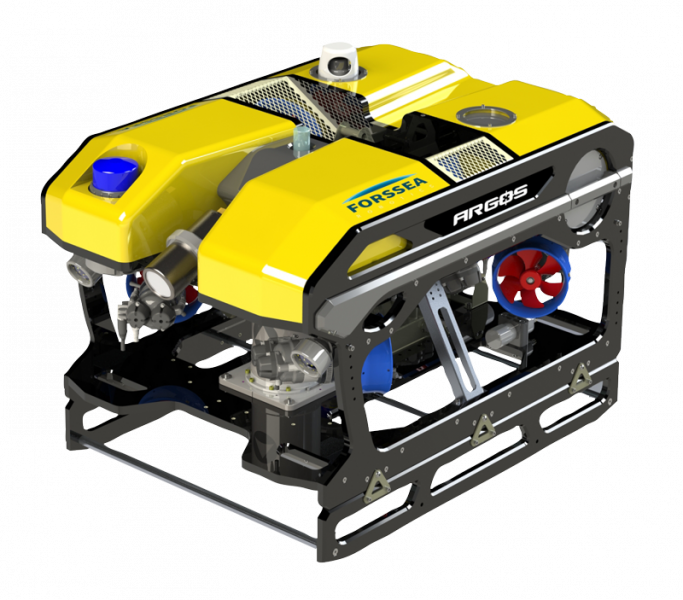
\includegraphics[width=\textwidth]{imgs/Argos.png}
					\caption{\argos{}}
				\end{subfigure}
				\hfill
				\begin{subfigure}[b]{0.3\textwidth}
					\centering
					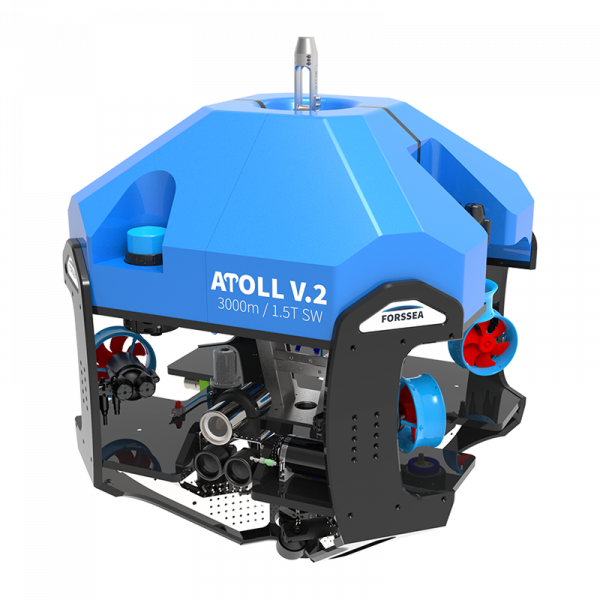
\includegraphics[width=\textwidth]{imgs/Atoll.png}
					\caption{\atoll{}}
				\end{subfigure}
				\hfill
				\begin{subfigure}[b]{0.3\textwidth}
					\centering
					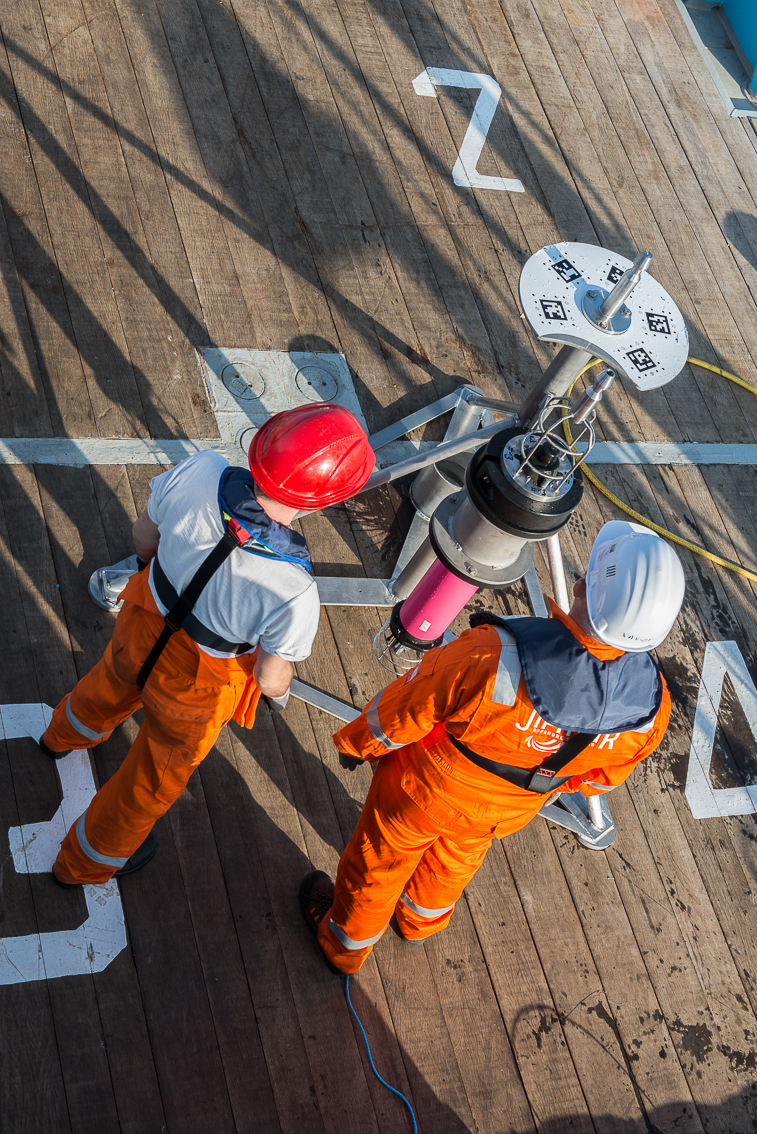
\includegraphics[width=\textwidth]{imgs/Frame.jpg}
					\caption{Structure sous-marine et balise}
				\end{subfigure}
				\caption{\gls{ROV}s proposés par \forssea{} et structure sous-marine}
				\label{fig:ROVs}
			\end{figure}

			Ils proposent aussi plusieurs solutions de captations visuelles\footnote{\url{https://forssea-robotics.fr/index.php/products/cameras}}. Il y a la \gls{Navcam} qui est une caméra embarquant des algorithmes de traitement permettant de réaliser du positionnement visuel, et l'\gls{Obscam} qui est une simple caméra étanche.

	\section[Projet de fin d'études]{Présentation du projet de fin d'études}

		\subsection{Cadre professionnel}

			Ce projet de fin d'étude s'inscrit dans le cadre d'un contrat de professionnalisation réalisé chez Forssea Robotics, entre octobre 2020 et octobre 2021. Il m'a permis d'effectuer un premier pas dans le monde industriel tout en finissant ma formation à l'\gls{ENSTAB}. J'ai donc pu avoir à ma charge un sujet plus complet étant donnée la durée de ce stage, mais j'ai aussi pu avoir plus de responsabilités dans la gestion de ce projet, dans la mesure ou j'ai intégré l'équipe robotique de \forssea{} pendant une année complète dont six mois à temps plein.

		\subsection{Présentation du sujet}

			Dans les phases de développements de ses \gls{ROV}s, \forssea{} doit faire face à de nombreuses problématiques, dont celle de tester les algorithmes implémentés sur les \gls{ROV}s. Pour cela l'entreprise réalise régulièrement des tests et conditions réelles, mais ce sont des essais coûteux et qui prennent beaucoup de temps à planifier et à organiser. Afin de réduire le nombre d'essais nécessaires, il serait préférable de développer un moyen de test rapide et fiable des robots dans leur environnement. Cela permettrait d'améliorer les performances des robots tout en diminuant les coûts et les temps de développements.

		\subsection{Objectifs du projet}

			L'objectif de ce stage est donc de construire un environnement de simulation sous-marin pour \forssea{}. Il devra permettre de simuler au mieux le comportement des robots dans leur milieu, mais aussi être interfaçable avec le reste de l'implémentation logicielle pour tester leurs algorithmes de navigations autonomes. Cet environnement de simulation doit aussi permettre de tester les \gls{ROV}s dans des situations qui peuvent être difficiles à mettre en place lors d'expérimentations. Il est tout de même à noter qu'aucun simulateur ne saurait remplacer la réalisation de tests en conditions réelles.

	
	\chapter{Conception et analyse du système}
\chaptermark{Système}
\label{chapitre:systeme}

    \section{Introduction}

        Dans ce chapitre nous allons réaliser les premières étapes de la conception du système de simulation. Dans un premier temps nous allons réliser une étude de l'existant afin de rendre compte des solutions permettant de simuler des environnements marins et sous-marins. Ensuite, nous allons établir les spécifications fonctionnelles de notre simulateur afin de définir les différentes fonctions que devra remplir notre système. Puis, nous allons élaborer les spécifications techniques de notre système, c'est à dire que nous allons déterminer les solutions techniques à employer afin de respecter le cahier des charges fonctionnelles. Enfin, nous seront en mesure de présenter une architecture logicielle pour notre simulateur, c'est-à-dire que nous allons présenter la manière dont vont s'agencer les différentes solutions techniques afin de produire le simulateur.

    \section{Etude de l'existant}

        La simulation de milieux marins est quelque chose de connu dans le domaine de la robotique, et il en existe aujourd'hui déjà de nombreux~\cite{Manhaes_2016, bingham19toward, MARS, Rock}. Ces simulateurs proposent tous un modèle de flottabilité pour les objets à simuler, ce qui permet de pouvoir définir à la fois des bateaux et des robots sous-marins. Cela permet donc de pouvoir simuler le comportement des \gls{ROV}s dans l'eau. Ils proposent ensuite tous leur lot de spécificités qui permettent d'avoir des éléments supplémentaires dans notre simulation.
        
        \textsc{UUV Simulator}~\cite{Manhaes_2016} est probablement le plus connu d'entre eux. C'est un simulateur de \gls{ROV} comportant un certain nombre d'éléments d'environnements simulés, comme des mondes marins, du courant ou des ombilicaux par exemple. Il propose aussi la description d'un bon nombre de robots sous-marins commercialisés, et la communauté active partage de nouveaux modèles régulièrement.
        
        \textsc{Mars}~\cite{MARS} est un simulateur spécifique à des robot baptisés \textsc{Mars}. Il permet de supporter plusieurs \gls{ROV}s et peut être commandé par \gls{ROS2} ou bien en utilisant des sockets TCP.
        
        \textsc{Rock-Gazebo}~\cite{Rock} est un projet d'intégration de simulateur basé sur le moteur physique \gazebo{} et sur le framework\footnote{Infrastructure logicielle facilitant le développement logiciel} \textsc{Robot Construction Kit}.
        
        Le simulateur \textsc{VRX}~\cite{bingham19toward} est un projet open-source de robotique marine dont un simulateur a été implémenté sur la base de \gazebo{}. Il propose un ensemble d'environnement, de modèles et de plugin permettant la simulation de missions de vaisseaux de surface, avec notamment la possibilité de prendre en compte la présence de vagues et de vent à la surface.

        Ces simulateurs proposent tous des spécificités différentes et intéressantes. Cependant, notre application de simulation de \gls{ROV}s pour \textsc{Forssea Robotics} est assez contrainte. En effet, l'existance de composants spécifiques, comme la simulation de structures sous-marines transportables rendent l'adaptation de simulateurs déjà existants trop difficile. C'est pourquoi il est nécéssaire de réaliser notre propre simulateur.

    \section{Spécifications fonctionnelles}
        \label{sec:spec_fonc}

        Le système à concevoir doit permettre de simuler \gls{ROV}s de la société \textsc{Forssea Robotics} dans un environnement sous-marin. Le simulateur doit respecter un certain nombre de spécifications fonctionnelles qui délimitent les exigences requises par le système. La \textsc{Figure}~\ref{figure:pieuvre} complétée par la \textsc{Table}~\ref{table:specs} présentent les exigences du système.

        \begin{figure}[!htb]
            \centering
            \begin{tikzpicture}[scale=0.7, every node/.style={ellipse, align=center, scale=0.7}]
                \node[draw,minimum height=40pt, minimum width=100pt, fill=VioletRed!70] (S) at (0, 0) {Simulateur};

                \node[draw,minimum height=40pt, minimum width=100pt, fill=Cerulean!80] (C0) at (0:5.5cm) {Robot};
                \node[draw,minimum height=40pt, minimum width=100pt, fill=Cerulean!80] (C1) at (72:2.8cm) {Environnement};
                \node[draw,minimum height=40pt, minimum width=100pt, fill=Cerulean!80] (C2) at (160:5cm) {Communication};
                \node[draw,minimum height=40pt, minimum width=100pt, fill=Cerulean!80] (C3) at (205:4.8cm) {Interface};
                \node[draw,minimum height=40pt, minimum width=100pt, fill=Cerulean!80] (C4) at (288:2.8cm) {Vizualisation};

                \draw[blue!75, line width=0.8mm] (C0) -- (S) node[midway, fill=white]{\textbf{FP1}};
                \draw[blue!75, line width=0.8mm] (C1) -- (S) node[midway, fill=white]{\textbf{FP2}};
                \draw[orange!80, line width=0.8mm] (C2) -- (S) node[midway, fill=white]{\textbf{FC1}};
                \draw[orange!80, line width=0.8mm] (C3) -- (S) node[midway, fill=white]{\textbf{FC2}};
                \draw[orange!80, line width=0.8mm] (C4) -- (S) node[midway, fill=white]{\textbf{FC3}};
            \end{tikzpicture}
            \caption{Diagramme pieuvre du système}
            \label{figure:pieuvre}
        \end{figure}

        \begin{table}[!htb]
            \centering
            \begin{adjustbox}{max width=\textwidth}
                \begin{tabularx}{\textwidth}{|lX|}
                    \hline
                    \cellcolor{gray!25}\textbf{id} & \cellcolor{gray!25} \textbf{Fonction} \\
                    \hline \hline
                    \cellcolor{blue!30}\textbf{FP1}&\cellcolor{blue!25} Le système doit avoir un comportement proche du robot réel. \\
                    \hline
                    \cellcolor{gray!10}FP1.1& Le système doit avoir des dimensions semblables au robot réel. \\
                    \hline
                    \cellcolor{gray!10}FP1.2& Le système doit avoir des masses et des inerties semblables au robot réel. \\
                    \hline
                    \cellcolor{gray!10}FP1.3& Le système doit avoir les mêmes degrès de liberté que le robot réel. \\
                    \hline
                    \cellcolor{gray!10}FP1.5& Le système doit avoir les mêmes actionneurs que le robot réel. \\
                    \hline
                    \cellcolor{gray!10}FP1.4& Le système doit avoir les mêmes capteurs que le robot réel. \\
            
                    \hline \hline
            
                    \cellcolor{blue!30}\textbf{FP2}&\cellcolor{blue!25} Le système doit simuler l'environnement marin et sous-marin du robot \\
                    \hline
                    \cellcolor{gray!10}FP2.1& Le système doit simuler l'eau et les vagues. \\
                    \hline
                    \cellcolor{gray!10}FP2.2& Le système doit simuler des courants marins. \\
                    \hline
                    \cellcolor{gray!10}FP2.3& Le système doit simuler les ombilicaux reliant le \gls{ROV} au bateau. \\
                    \hline
                    \cellcolor{gray!10}FP2.4& Le système doit simuler les structures sous marines à transporter. \\
                    \hline
            
                    \hline \hline
            
                    \cellcolor{orange!40}\textbf{FC1} &\cellcolor{orange!30} Le système doit communiquer son état à l'utilisateur. \\
                    \hline
                    \cellcolor{gray!10}FC1.1& Le système doit communiquer l'état du robot à l'utilisateur. \\
                    \hline
                    \cellcolor{gray!10}FC1.2& Le système doit communiquer l'état de l'environnement à l'utilisateur.\\
                    \hline
            
                    \hline \hline
            
                    \cellcolor{orange!40}\textbf{FC2}&\cellcolor{orange!30} Le système doit être interfaceable avec le reste de l'implémentation logicielle. \\
                    \hline
                    \cellcolor{gray!10}FC2.1& Le système doit communiquer avec l'implémentation logicielle en \gls{ROS2}. \\
                    \hline
                    \cellcolor{gray!10}FC2.2& Le système doit être pilotable par les contrôleurs utilisés pour les robots réels. \\
                    \hline

                    \hline \hline
            
                    \cellcolor{orange!40}\textbf{FC3}&\cellcolor{orange!30} Le système doit être visualisable par l'utilisateur. \\
                    \hline
                    \cellcolor{gray!10}FC3.1& Le système doit pouvoir représenter les \gls{ROV}s dans leur environnement au cours de la simulation. \\
                    \hline
                    \cellcolor{gray!10}FC3.2& Le système doit fournir l'état des \gls{ROV}s et de l'environnement à l'utilisateur.  \\
                    \hline
                \end{tabularx}
            \end{adjustbox}
            \caption{Spécifications fonctionnelles du simulateur}
            \label{table:specs}
        \end{table}    

    \section{Spécifications techniques}

        Pour remplir les différentes spécifications fonctionnelles présentées dans la \textsc{Section}~\ref{sec:spec_fonc}, nous allons définir un certain nombre de spécifications techniques. Ces dernières vont proposer les outils et les différents critères permettant de remplir les exigences attendues.

        \subsection{Logiciel de simulation}

            L'étude de l'existant nous aura au moins permis de se rendre compte que \gazebo{}~\cite{Koenig-gazebo} est largement utilisé dans le domaine de la simulation sous-marine, mais aussi plus largement dans la simulation robotique. \gazebo{} est un logiciel de simulation multi-physique \textit{open-source}\footnote{Code communautaire ouvert libre de redistribution et d'accès}. Il est aujourd'hui développé par la communauté \textit{Open Robotics}\footnote{\url{https://www.openrobotics.org/}}.
            
            Il est possible de décrire précisément les robots, c'est-à-dire de décrire les couches visuelles, d'inerties et de collisions des robots afin de les simuler dans \gazebo{} en utilisant le language \gls{SDF}\footnote{\url{http://sdformat.org/}}. Pour décrire le comportement de composants plus complexes comme des capteurs ou des actionneurs, un système de \textit{plugins} est disponible afin de laisser les développeurs ajouter des fonctionnalités à \gazebo{}. Ainsi la fonction principale \textbf{FP1} est remplie, car on est en mesure de simuler les robots avec des paramètres mécaniques proches du robot réel.

            De même, l'environnement est décrit à l'aide du language \gls{SDF} et un système de \textit{plugins} permet d'intéragir avec l'environnement de simulation afin d'ajouter des forces, des couples, ou bien des marqueurs visuels par exmple. Cela permet de remplir la fonction principale \textbf{FP2}.

            Ensuite, l'état du système est directement visualisable sur \gazebo{}. En effet, ce logiciel réalise la simulation et montre les robots évoluants dans leur environnement simulé, ce qui permet aussi de remplir une partie de la fonction contrainte \textbf{FC1}.

            Enfin, ce logiciel présente l'avantage de pouvoir communiquer avec \gls{ROS2}, ce qui satisfait la fonction contrainte \textbf{FC2}, en interfaçant le simulateur avec le reste de l'implémentation logicielle des robots.

        \subsection{Ignition Libraries}

            \textit{Ignition Libraries}\footnote{\url{https://ignitionrobotics.org/libs}} est un ensemble de libraries permettant de faciliter le développement robotique. Deux libraries permettent de compléter la fonction contrainte \textbf{FC1} : \textit{Ignition-Transport} et \textit{Ignition-Msgs}. Elles permettent de faire communiquer deux parties de codes ensemble grâce à un système de messagerie basée sur l'utilisation de la bibliothèque \textit{ProtocolBuffer} développée par \textit{Google}\footnote{\url{https://developers.google.com/protocol-buffers}}. C'est le même système de communication qui est utilisé par \gls{ROS2} et \gazebo{}. Ce système de communication présente l'avantage de diviser le code en n\oe uds pouvant s'exécuter en parallèle et communiquant ensemble par ces librairies, mais aussi de pouvoir récupérer l'état du simulateur par la lecture des messages transitants sur le réseau \textit{Ignition-Transport}. Ainsi on peut précisément savoir ce qu'il se passe dans le simulateur à cahque instant.

        \subsection{ROS2 Control}

            Pour respecter la fonction contrainte \textbf{FC2}, le simulateur doit s'interfacer avec le reste de l'implémentation logicielle, il est donc nécéssaire de définir une architecture logicielle permettant de communiquer à la fois avec les \gls{ROV}s réels et simulés. \gls{ROS2Control}~\cite{ros_control} est un framework permettant de faire communiquer des contrôleurs et des drivers ensemble. Le principal avantage est qu'il est temps-réel, c'est-à-dire que les données des capteurs sont accessible instantanément par les contrôleurs, les actionneurs ont aussi instantanément accès aux commandes, et enfin on peut changer de manière consistante de contrôleur, sans temps mort durant lesquels le robot ne serait pas commandé.

            \begin{figure}[!htb]
                \centering
                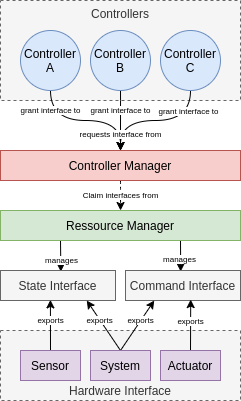
\includegraphics{imgs/ros2_control.pdf}
                \caption{Architecture logicielle avec \gls{ROS2Control}}
                \label{fig:ros2_control}
            \end{figure}

            La \textsc{Figure}~\ref{fig:ros2_control} nous montre l'architecture logicielle de \gls{ROS2Control}. Ce framework va instancier un \textit{Controller Manager} qui va s'occuper de charger les contrôleurs qui seront utilisés dans le robot, des \textit{Hardware Interface} qui sont les interfaces qui vont communiquer avec les composants et un \textit{Ressource Manager} qui va faire transiter les données entre les contrôleurs et les composants. L'\textit{Hardware Interface} peut avoir pour rôle de communiquer avec les composants réels, où avec les composants simulés. L'idée est de créer une \textit{Hardware Interface} pour la simulation proposant les mêmes interfaces que celle implémentée pour les composants réels. Ainsi on peut utiliser les mêmes algorithmes de contrôle de manière totalement transparente pour commander le robot réel ou le simulateur, et la fonction contrainte \textbf{FC2} est remplie.

        \subsection{Architecture Logicielle}

            En rassemblant ce qui a pu être présenté dans cette chapitre, on peut proposer l'architecture logicielle présentée sur la \textsc{Figure}~\ref{fig:architecture_logicielle} pour ce simulateur.
            
            Ce système nécessite donc dans un premier la description pour \gazebo{} d'un monde de simulation sous-marin ainsi que la description des \gls{ROV}s dans un premier temps afin de pouvoir simuler les robots. Puis vient l'implémentation de \textit{plugins} \gazebo{} et d'\textit{Hardware Interface} pour interagir et controller ces robots, qui communique ensemble par le biai des librairies fournies par \textit{ignition robotics}.
            
            \begin{figure}[!htb]
                \centering
                \includegraphics[]{imgs/architecture_logicielle.pdf}
                \caption{Architecture logicielle du simulateur}
                \label{fig:architecture_logicielle}
            \end{figure}

    \section{Conclusion}

        En conlusion, nous avons défini dans ce chapitre les exigences attendues pour ce simulateur. Elles nous ont permis de choisir des solutions techniques adaptées à la réalisation de ce système et nous avons donc pu proposer une architecture logicielle à mettre en place pour simuler correctement les \gls{ROV}s de \textit{Forssea Robotics}. Nous allons donc pouvoir commencer le développement de ce système en utilisant les outils mis en place dans ce chapitre.
        
	\chapter{Simulation de l'environnement}
\chaptermark{Environnement}
\label{chapitre:environnement}
	
	\section{Introduction}

		Dans ce chapitre, nous allons nous intéresser à la simulation de l'environnement. Elle constitue une partie importante du simulateur car elle va influencer le comportement des \gls{ROV}s dans leur milieu.  A la fin de ce chapitre, nous devrions avoir à notre disposition un environnement de simulation complet proche de l'environnement rencontré lors de missions avec les robots.

		Pour ce faire, nous allons donc d'établir les différents éléments de l'environnement qui vont interagir avec les \gls{ROV}s afin de les intégrer dans le simulateur. Ce qui va principalement influencer le comportement des robots est le milieu marin qui va ajouter la flottabilité, les vagues et des courants marins. Nous allons aussi nous intéresser aux ombilicaux qui relient les \gls{ROV}s au bateau afin de l'alimenter en énergie mais aussi d'avoir un retour d'informations.
		
	\section{Environnement marin}

		\subsection{Introduction}
			
			La simulation de l'environnement marin est probablement ce qui va le plus impacter le comportement des \gls{ROV}s. Le milieu marin doit proposer un modèle de mer avec des vagues, ajouter de la flottabilité aux robots et simuler du courant.

		\subsection{Modélisation de la surface libre}

			\subsubsection{Introduction}

				Dans un premier temps, nous allons nous intéresser à la modélisation de la surface libre de la mer, c’est-à-dire qu'il nous faut trouver un formalisme permettant de simuler la surface de l'environnement marin, à l'interface entre l'air et l'eau.

				Les premières modélisations de la mer étaient des champs de hauteur, c’est-à-dire que pour chaque $(x, y)$ dans le plan de la mer, on y associait au maximum un $z$. Cette modélisation peut aux premiers abords suffire, et elle a d'ailleurs été utilisée pour réaliser les premiers rendus informatiques de mer~\cite{scha80, max81}, comme celui présenté sur la \textsc{Figure}~\ref{fig:carlas_island}. Mais on se rend compte qu'en réalité un champ de hauteur ne suffit pas. En effet, pour décrire une mer comme celle présentée en \textsc{Figure}~\ref{fig:hokusai}, il faut établir l'équation paramétrique de la surface libre, car pour un même couple $(x, y)$ il est possible d'avoir plusieurs $z$ associés si les vagues roulent les unes sur les autres.

				\begin{figure}[!htb]
					\centering
					\begin{subfigure}[t]{0.48\textwidth}
						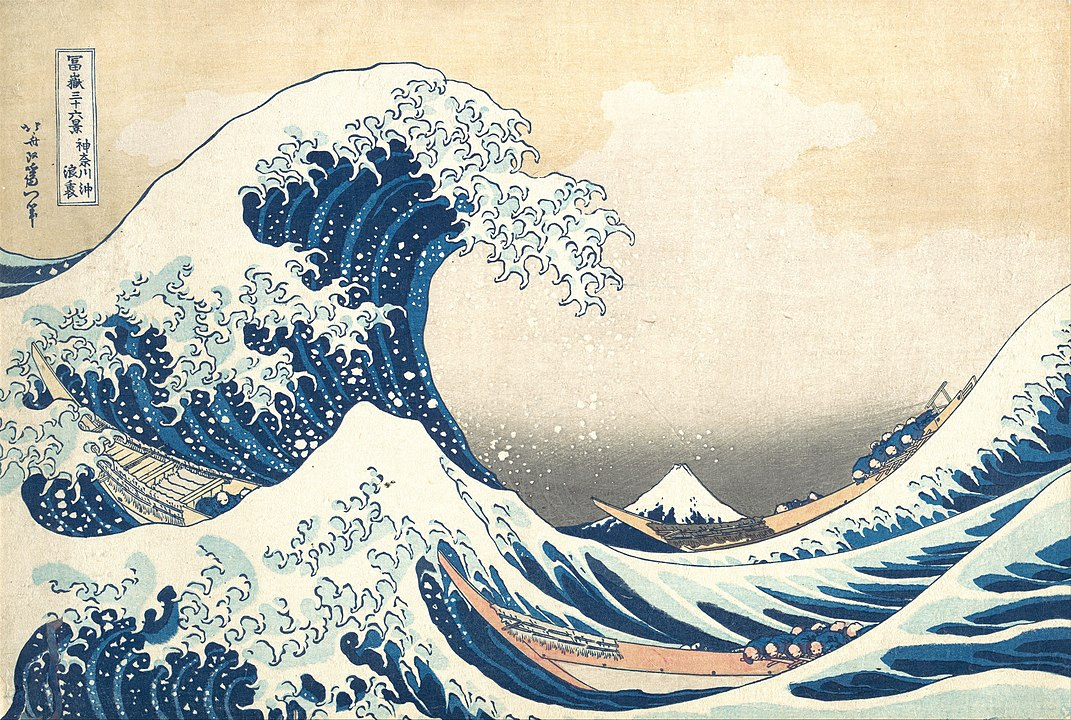
\includegraphics[width=\textwidth]{imgs/tsunami_hokusai.jpg}
						\caption{La grande vague de Kanagawa, Katsushika Hokusai, 1830~\cite{hokusai_1830}}
						\label{fig:hokusai}
					\end{subfigure}
					\begin{subfigure}[t]{0.5\textwidth}
						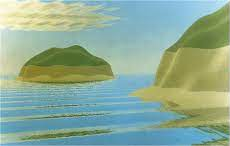
\includegraphics[width=\textwidth]{imgs/carlas_island.png}
						\caption{Carla's Island, Max Nelson L., 1981~\cite{max81}}
						\label{fig:carlas_island}
					\end{subfigure}
					\caption{Représentation de la surface libre de la mer}
					\label{fig:representation_mer}
				\end{figure}

				Un modèle établi il y a plus de deux cents par \textit{Gerstner}~\cite{Gerstner} propose une modélisation trochoïdale de la houle. Cette modélisation permet de décrire la forme de la surface libre de l'eau. Cependant elle n'est vraie qu'en eaux profondes, et cette description se concentre sur des vagues dans un plan en deux dimensions $(0, \overrightarrow{x}, \overrightarrow{z})$, avec x orienté dans le sens de propagation de la vague, et z orienté vers le haut. Dans le cas plus général, il est possible d'étendre ce modèle à un environnement en trois dimensions~\cite{Constantin_2001, Gerstner-Like_Henry}, qui est aussi connu sous le nom d'\textit{Airy Wave}, et même à un modèle en eaux peu profondes ou semi-profondes~\cite{dean1991water}. Cette modélisation présente l'avantage d'être linéaire. Il faut cependant s'assurer que les vagues ne déferlent pas afin de ne pas entrer dans le domaine non-linéaire, comme présenté sur la \textsc{Figure}~\ref{fig:hokusai} représentant un tsunami avec des vagues déferlantes. D'après l'échelle de \textit{Beaufort}~\cite{beaufort}, le modèle de vagues linéaire semble acceptable jusqu'à \textit{mer 3}, car au-delà des moutons blancs apparaissent à la surface de la mer et les vagues commencent à déferler. Nous nous limiterons donc à ce domaine pour la simulation de l'environnement, d'autant plus que les robots ne sortent pas en milieu naturel par \textit{mer 4} et au-delà.

			\subsubsection{Formalisme}

				Plaçons-nous dans un repère $(0, \overrightarrow{x}, \overrightarrow{y}, \overrightarrow{z})$ tel que $0$ soit au niveau de la mer au repos, $\overrightarrow{x}$ soit orienté dans le sens de déplacement de la vague, $\overrightarrow{z}$ orienté vers le haut, et $\overrightarrow{y}$ tel que la base formée soit un repère direct. La \textsc{Figure}~\ref{fig:repere} représente une vague dans le repère de l'étude.

				\begin{figure}[!htb]
					\centering
					\begin{tikzpicture}[x={(20:1cm)},y={(90:1cm)},z={(160:1cm)},line join=round,]
							\tikzset{xyp/.style={canvas is xy plane at z=#1}}

							\filldraw[brown!50,draw=black] (0,0,0) -- (3,0,0) -- (3,0.3,0) -- cycle;
							\filldraw[brown!50,draw=black] (0,0,0) -- (3,0.3,0) -- (3,0.3,1.5) -- (0,0,1.5) -- cycle;
							\draw[blue!50!cyan!50!black,thick] (1.5,1,0) -- (1.5,1,1.5);
						
							\foreach \z in {50, ..., 0}
							{   \pgfmathsetmacro{\drawperc}{or(\z==0,\z==50) ? 1 : 0}
								\ifthenelse{\z=0 \OR \z=50}
								{   \gdef\myc{blue!50!cyan!50!black}}
								{ \gdef\myc{blue!30!cyan!30!white}}
								\filldraw[blue!30!cyan!30!white,xyp=\z/100*3,opacity=1,draw=\myc,draw opacity=1] (0,0) -- (3,0.3) -- (3,1) to[out=170,in=0,looseness=1] (1.5,2) to[out=180,in=20] (0,1.5) -- cycle;
							}
						
							\draw[blue!50!cyan!50!black] (0,1.5,0) -- (0,1.5,1.5) -- (0,0,1.5) --(0,0,0);

							\draw[draw=black, fill=gray, opacity=0.2] (0, 0, 0) -- (0, 2.5, 0) -- (3, 2.5, 0) -- (3, 0, 0) -- cycle;
							\draw[draw=black, dotted] (0,1.5,0) node[below left] {$O$} -- (3,1.5,0) -- (3,1.5,1.5) -- (0,1.5,1.5) -- cycle;
							\draw[->, >=stealth, color=red, thick] (0,1.5,0) -- (0.8,1.5,0) node[below right] {$\overrightarrow{x}$};
							\draw[->, >=stealth, color=ForestGreen, thick] (0,1.5,0) -- (0,1.5,0.8) node[below left] {$\overrightarrow{y}$};
  							\draw[->, >=stealth, color=NavyBlue, thick] (0,1.5,0) -- (0,2.3,0) node[above right] {$\overrightarrow{z}$};
						\end{tikzpicture}
						\caption{Modélisation de la vague et repère de l'étude}
						\label{fig:repere}
				\end{figure}


				Cette modélisation de houle trochoïdale utilise une approche lagrangienne pour définir l'équation paramétrique de la surface libre~\cite{Gerstner, Constantin_2001, Gerstner-Like_Henry, dean1991water}. On s'intéresse donc à une particule de fluide positionnée au repos en $p_0=(\alpha, \beta, 0)$, à l'instant $t$, au-dessus d'une colonne d'eau de hauteur $H$. Chaque vague trochoïdale $m$ est ensuite définie par son amplitude $a_m$, son nombre d'onde $k_m$, sa phase $\phi_m$ et sa pulsation $\omega_m$ et va influencer la position de cette particule au cours du temps comme suit :

				\begin{eqnarray}
					\xi(\alpha, \beta, t) & = & \alpha - \sum_{m=0}^{M} \frac{k_{x, m}}{k_m} \cdot \frac{a_m}{tanh(k_m H)} \cdot sin(\theta_m) \label{eqn:xi}\\ 
					\zeta(\alpha, \beta, t) & = & \beta - \sum_{m=0}^{M} \frac{k_{y, m}}{k_m} \cdot \frac{a_m}{tanh(k_m H)} \cdot sin(\theta_m) \label{eqn:zeta}\\ 
					\eta(\alpha, \beta, t) & = & - \sum_{m=0}^{M} a_m \cdot cos(\theta_m) \label{eqn:eta}\\ 
					\theta_m(\alpha, \beta, t) & = & k_{x, m} \alpha + k_{z, m} \beta - \omega_m t - \phi_m \label{eqn:theta}
				\end{eqnarray}

				On a alors défini l'équation paramétrique de la surface libre de l'eau $x = \xi(\alpha, \beta, t)$, $y = \zeta(\alpha, \beta, t)$, et $z = \eta(\alpha, \beta, t)$. La relation de dispersion relie la pulsation $\omega_m$ de chaque signal au nombre d'onde $k_m$, et $k_{x, m}$ et $k_{y, m}$ sont les composantes du vecteur nombre d'ondes dans le plan de la mer tel que  :
				
				\begin{eqnarray}
					\omega_m^2 & = & g \cdot k_m \cdot tanh(k_m H) \label{equation:dispersion} \\
					k_m & = & \sqrt{k_{x, m}^2 + k_{y, m}^2} \label{equation:nombre_onde}
				\end{eqnarray}

				Dès lors, il est possible de définir $k_{x, m}$ et $k_{y, m}$ en introduisant le cap de la vague $h_m$ par rapport au repère présenté en \textsc{Figure}~\ref{fig:repere} :

				\begin{eqnarray}
					k_{x, m} & = & cos(h_m) \cdot k_m \\
					k_{y, m} & = & sin(h_m) \cdot k_m \\
				\end{eqnarray}

				Ainsi les expressions de $k_{x, m}$ et $k_{y, m}$ vérifient l'\textsc{Equation}~\ref{equation:nombre_onde} et sont calculées uniquement à partir des valeurs de $k_m$ et de $h_m$.
				
				La forme de la vague est définie par les différents paramètres de la vague. On peut par exemple s'intéresser au produit adimensionné $a_m\cdot k_m$. La \textsc{Figure}~\ref{fig:amkm} présente le profil d'une vague pour un produit valant $0.1$ un autre égal à $1$, et un dernier valant $1.2$. On se rend compte que jusqu'à une valeur de $1$ les vagues sont réalistes, mais qu'au-delà, une boucle se forme. C'est à cet endroit que le modèle linéaire des vagues s'arrête, car la crête va en réalité s'effondrer au lieu de former une boucle, la vague va déferler et de l'écume va s'y former~\cite{Gerstner-Like_Henry, Gerstner_Pixar}. On veillera donc à ne pas dépasser cette valeur charnière afin de rester dans le domaine linéaire, mais aussi afin d'avoir une simulation réaliste.

				\begin{figure}[!htb]
					\centering
					\includegraphics{build/imgs/gerstner_wave.pdf}
					\caption{Vagues de Gerstner pour différentes valeurs de $a_m\cdot k_m$}
					\label{fig:amkm}
				\end{figure}

				Enfin, une amélioration proposée par A. \textsc{Fournier}~\cite{Gerstner_Pixar} est d'ajouter un terme sur la phase permettant de faire accélérer les crêtes de vagues, et de faire ralentir les creux. C'est quelque chose que l'on retrouve réellement sur les vagues, et cela permet d'orienter les vagues suivant la direction de leur déplacement. L'\textsc{Equation}~\ref{equation:pixar_phase} donne la nouvelle expression de la phase. Le terme ajouté introduit un paramètre $\gamma_m$ permettant de gérer l'intensité de l'effet ajouté, et $z$ qui est la hauteur de la particule considérée. L'effet est réparti linéairement suivant la hauteur de la vague, et en $z=0$ aucun changement de phase n'a lieu car le terme s'annule. La \textsc{Figure}~\ref{fig:gerstner_pixar} montre comment l'ajout de ce paramètre de phase agit sur la forme de la vague.

				\begin{equation}
					\theta_m(\alpha, \beta, t) = k_{x, m} \alpha + k_{z, m} \beta - \omega_m t - \phi_m - \gamma_m z
					\label{equation:pixar_phase}
				\end{equation}

				\begin{figure}[!htb]
					\centering
					\includegraphics{build/imgs/gerstner_pixar.pdf}
					\caption{Forme de la vague en fonction du paramètre $\gamma_m$}
					\label{fig:gerstner_pixar}
				\end{figure}

				Cependant, si ce modèle suffit à représenter la surface libre de la mer, il ne fournit pas la dynamique du milieu marin et l'impact qu'il va voir sur les \gls{ROV}s. C'est pourquoi il va falloir établir les équations de vitesse des particules et de pression afin de pouvoir pleinement simuler le milieu marin.
				
			\subsubsection{Dynamique du milieu}

				Après avoir défini la forme de la surface libre de la mer, il faut désormais établir les équations du mouvement des particules de fluides dans l'eau~\cite{dean1991water, MIT_Waves}. Il faut notamment définir leur position notée $(x, y, z)$, leur vitesse notée $(u, v, w)$, et établir l'équation de pression notée $p$. La hauteur $z$ étant prise par rapport au repère présenté en \textsc{Figure}~\ref{fig:repere}, cette valeur est souvent négative, sauf quand une vague élève localement le niveau de l'eau au-dessus du niveau nul.

				En continuant à utiliser le formalisme précédemment introduit, on est en mesure d'étendre les \textsc{Equations}~\ref{eqn:xi} à \ref{eqn:eta} à tous les points de l'espace immergés en s'aidant des références bibliographiques~\cite{dean1991water, MIT_Waves} :

				\begin{eqnarray}
					\xi(\alpha, \beta, z, t) & = & \alpha - cos(h_m) \sum_{m=0}^{M} a_m \cdot \frac{cosh(k_m(z+H))}{sinh(k_m H)} \cdot sin(\theta_m) \\
					\zeta(\alpha, \beta, z, t) & = & \beta - sin(h_m) \sum_{m=0}^{M} a_m \cdot \frac{cosh(k_m(z+H))}{sinh(k_m H)} \cdot sin(\theta_m) \\
					\eta(\alpha, \beta, z, t) & = & z - \sum_{m=0}^{M} \frac{a_m}{k_m} \cdot \frac{sinh(k_m(z+H))}{sinh(k_mh)} \cdot cos(\theta_m)
				\end{eqnarray}

				Puis, on peut établir les équations de vitesse des particules de la même manière, en dérivant temporellement les équations de positions :
		
				\begin{eqnarray}
					v(\alpha, \beta, z, t) & = & sin(h_m) \sum_{m=0}^{M} a_m \cdot \omega_m \cdot \frac{cosh(k_m(z+H))}{sinh(k_m H)} \cdot cos(\theta_m) \\
					u(\alpha, \beta, z, t) & = & cos(h_m) \sum_{m=0}^{M} a_m \cdot \omega_m \cdot \frac{cosh(k_m(z+H))}{sinh(k_m H)} \cdot cos(\theta_m) \\
					w(\alpha, \beta, z, t) & = & - \sum_{m=0}^{M} \frac{a_m}{k_m} \cdot \omega_m \cdot \frac{sinh(k_m(z+H))}{sinh(k_m H)} \cdot sin(\theta_m)
				\end{eqnarray}

				Enfin, il nous reste à établir l'équation de pression :

				\begin{equation}
					p(\alpha, \beta, z, t) = \rho \sum_{m=0}^{M} \frac{a_m\omega_m^2}{k} \cdot \frac{cosh(k_m(z+H))}{sinh(k_m H)} \cdot cos(\theta_m) - \rho g z
				\end{equation}

				Ces équations prennent en compte l'impact significatif de la hauteur de la colonne d'eau dans le cas où les vagues sont présentes dans un milieu de faible profondeur. De plus, il est intéressant de remarquer que l'impact des vagues sur la dynamique des particules diminue quand la profondeur augmente, comme le montre la \textsc{Figure}~\ref{fig:speed_pressure_depth}. Cet effet se trouve dans les termes en cosinus et sinus hyperboliques qui décroissent très vite vers 0 quand on s'approche du fond, et qui valent 1 en $z=0$. Ainsi on remarque que la vitesse des particules décroit rapidement vers une vitesse nulle à mesure que la profondeur augmente et la pression n'est impactée que proche de la surface où elle est légèrement supérieure à la pression qu'il y aurait eu sans vagues.

				\begin{figure}[!htb]
					\centering
					\includegraphics[]{build/imgs/gerstner_velocity_pressure_depth.pdf}
					\caption{Evolution de la vitesse des particules et de la pression en fonction de la profondeur à $t=0$, $\alpha=0$ et $\beta=0$, pour une vague d'amplitude $a_m=1\ m$ et de nombre d'onde $k_m = 1\ rad.m^{-1}$}
					\label{fig:speed_pressure_depth}
				\end{figure}

			\subsubsection{Simplification en eaux profondes}
			\label{sec:simplification_eaux_profondes}
			
				Finalement, on peut simplifier le modèle précédent, en remarquant que la hauteur de la colonne d'eau dans notre cas est très grande devant la longueur d'onde caractéristique de nos vagues. Une explication plus détaillée de la simplification est disponible en \textsc{Annexe}~\ref{annexe:deep_water}. On déduit de cette simplification, que pour une hauteur de colonne d'eau très grande devant la longueur d'onde des vagues :

				\begin{equation}\frac{cosh(k_m(z+H))}{sinh(k_mH)} \approx e^{k_mz} \label{eqn:simplification_eaux_profondes}\end{equation}

				Comme $z$ est négatif sous la surface de l'eau, ce terme est une exponentielle décroissante qui va atténuer fortement l'effet des vagues au fond et avoir un effet plus conséquent sur les premiers mètres d'eau. On peut montrer que la distance caractéristique d'atténuation est de l'ordre d'une demi-longueur d'onde. En effet, en notant $\lambda_m$ la longueur d'onde de la vague, on a $k_m = \tfrac{2\pi}{\lambda_m}$, et en évaluant l'expression en $z = - \tfrac{\lambda_m}{2}$, $e^{-\tfrac{k_m\lambda_m}{2}} = e^{-\pi} \approx 0,05$. Cela signifie que $95 \%$ de l'effet des vagues est dissipé sur une demi-longueur d'onde de profondeur. Avec cette simplification, les équations de position se simplifient comme suit :
			
				\begin{eqnarray}
					\xi(\alpha, \beta, z, t) & = & \alpha - cos(h_m) \sum_{m=0}^M a_m \cdot e^{k_mz} \cdot sin(\theta_m) \\
					\zeta(\alpha, \beta, z, t) & = & \beta - sin(h_m) \sum_{m=0}^M a_m \cdot e^{k_mz} \cdot sin(\theta_m) \\
					\eta(\alpha, \beta, z, t) & = & z - \sum_{m=0}^M a_m \cdot e^{k_mz} \cdot cos(\theta_m) \\
				\end{eqnarray}

				Les équations de vitesse des particules de fluides se simplifient comme suit :

				\begin{eqnarray}
					u(\alpha, \beta, z, t) & = & cos(h_m) \sum_{m=0}^M a_m \cdot \omega_m \cdot e^{k_mz} \cdot cos(\theta_m) \\
					u(\alpha, \beta, z, t) & = & sin(h_m) \sum_{m=0}^M a_m \cdot \omega_m \cdot e^{k_mz} \cdot cos(\theta_m) \\
					w(\alpha, \beta, z, t) & = & - \sum_{m=0}^M a_m \cdot \omega_m \cdot e^{k_mz} \cdot sin(\theta_m) \\
				\end{eqnarray}

				Pour l'équation de pression au sein du milieu et l'équation de dispersion qui lie la pulsation de la vague à son nombre d'onde, elles se simplifient comme suit :

				\begin{eqnarray}
					p(\alpha, \beta, z, t) & = & \rho g \sum_{m=0}^M a_m \cdot e^{k_mz} \cdot cos(\theta_m) - \rho g z\\
					\omega_m^2 & = & k_m g \label{equation:deep_dispersion}
				\end{eqnarray}

			\subsubsection{Choix du spectre de vagues}

				L'avantage de cette modélisation linéaire des vagues est qu'il est possible d'additionner des vagues de caractéristiques différentes en utilisant le principe de superposition. Ainsi on peut définir un environnement marin réaliste en ajoutant l'effet de plusieurs vagues sur les particules de fluides. L'idée va donc être de définir une vague principale,avec une amplitude de l'ordre du mètre, qui aura donc un très faible nombre d'onde pour respecter la condition $a_m \cdot k_m \le 1$. Puis, on ajoute à cette vague des vaguelettes d'amplitudes moindres qui auront des nombres d'ondes plus élevées afin de rider la surface de l'eau et d'obtenir un résultat réaliste.

				Pour une optimisation en termes de calculs, il est possible de prendre des nombres d'ondes tombant sur la grille qui va servir de support pour réaliser le rendu de la surface libre~\cite{tessendorf2001simulating}. Par la relation de dispersion, cela va créer des vagues avec des pulsations multiples les unes des autres, ce qui va permettre d'avoir un phénomène périodique. Il est donc possible de pré-calculer sur une période tous les paramètres dynamiques de l'environnement, et ainsi de baisser la charge de calculs lors de la simulation. Pour notre cas cela ne sera pas nécessaire, d'abord car la charge de calculs demandée ne ralentit pas la simulation, mais aussi car nous ne voulons pas forcément nous limiter à un phénomène de vagues périodiques.
			
			\subsubsection{Implémentation de la solution}

				Cette modélisation a menée à l'implémentation d'une classe contenant tous les paramètres des vagues de l'environnement. Elle permet de réaliser tous les calculs nécessaires à la simulation visuelle et dynamique du milieu marin modélisé. Cette classe est ensuite instanciée par un \textit{plugin} \gazebo{} de type \textit{WorldPlugin} qui s'applique donc sur le monde simulé, et qui a pour rôle de publier les paramètres du monde marin sur le réseau de communication \textit{ignition transport}, mais aussi de répondre aux requêtes envoyées par d'autres plugins sur la dynamique de l'eau à une certaine position passée en paramètre. 
				
				Pour réaliser le rendu visuel de la mer, on peut créer une grille de particules de fluides pour laquelle on va pouvoir réaliser le rendu de la position au cours du temps. A chaque instant, on actualise la position de chaque particule de fluide et on trace à nouveau la grille. On est alors en mesure d'obtenir le résultat visualisable en \textsc{Figure}~\ref{fig:Gerstner} dans \gazebo{}, obtenu à l'aide de trois vagues dont les caractéristiques sont présentées dans la \textsc{Table}~\ref{table:wave} et tracé sur une grille de 40 mètres par 40 mètres avec un pas de 1 mètre. Les paramètres des vagues ainsi que de la grille de rendu sont passées en paramètre au \plugin{} implémenté afin de pouvoir rapidement plonger les \gls{ROV}s dans des milieux ayant des dynamiques différentes.

				\begin{figure}[!htb]
					\begin{minipage}[c]{0.45\textwidth}
						\centering
						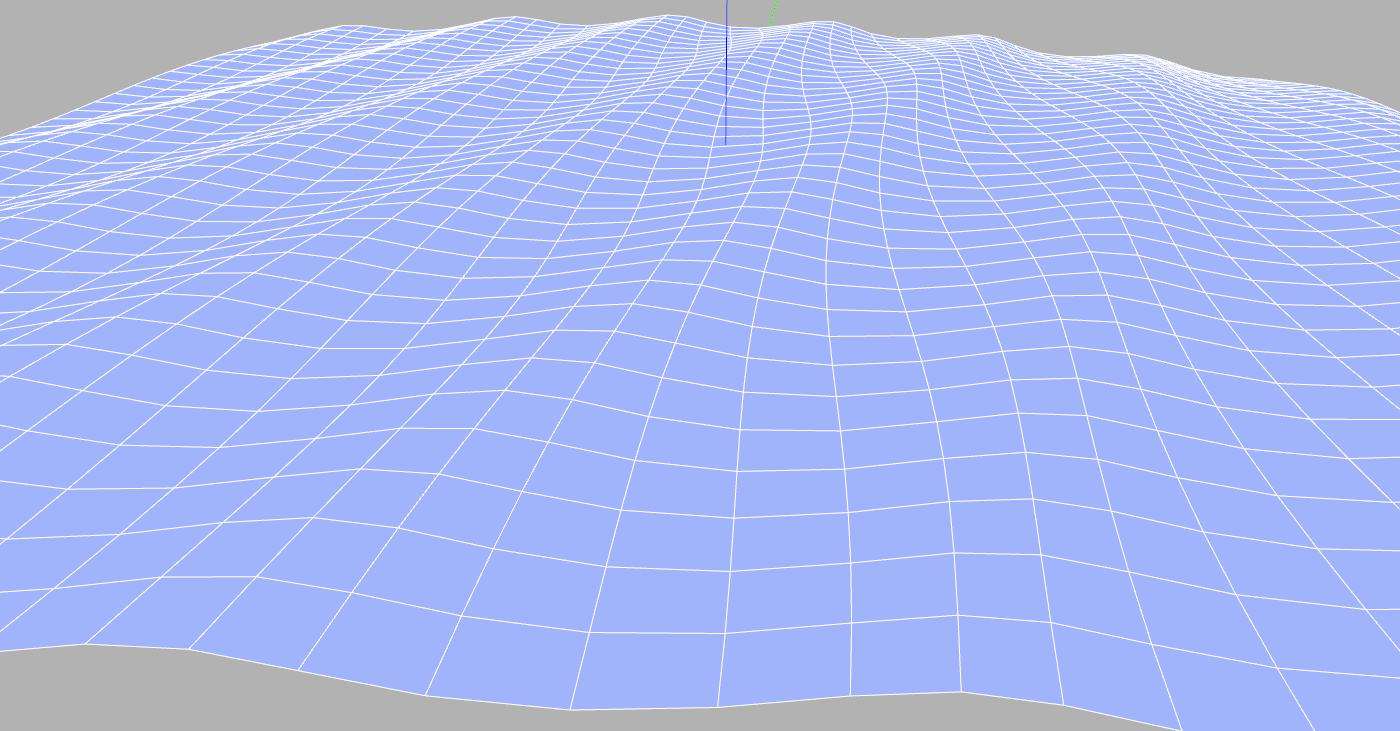
\includegraphics[width=\textwidth]{imgs/gerstner.jpg}
						\caption{Vagues dans \gazebo{}}
						\label{fig:Gerstner}
					\end{minipage} \hfill
					\begin{minipage}[c]{0.54\textwidth}
						\centering
						\begin{adjustbox}{max width=\textwidth}
							\begin{tabular}{c c c c c c}
								\toprule
								\textbf{Vague} & $a_m$ ($m$) & $k_m$ ($rad.m^{-1}$) & $\phi_m$ ($rad$) & $h_m$ ($rad$) & $\gamma_m (rad.m^{-1})$ \\
								\midrule
								Vague 1 & 1.2 & 0.06 & 0 & 0 & 0.5\\
								Vague 2 & 0.6 & 0.1 & 0 & 0.8 & 0.3\\
								Vague 3 & 0.2 & 1 & 0 & -0.3 & 0\\
								\bottomrule
							\end{tabular}
						\end{adjustbox}
						\caption{Caractéristiques des vagues simulées}
						\label{table:wave}
					\end{minipage}
				\end{figure}

		\subsection{Forces induites par le milieu}

			\subsubsection{Introduction}
			
				Les forces qui s'appliquent sur un solide immergé dans un fluide en mouvement sont la poussée d'Archimède~\cite{dean1991water}, les forces de Morison~\cite{morison1950force, dean1991water} et celles de Froude-Krylov~\cite{dean1991water}. Elles permettent d'appliquer les forces que subit les objets immergés. Les forces de Morison et les forces de Froude-Krylov possèdent cependant quelques limitations~\cite{dean1991water, sarpkaya2010wave} :

				\begin{itemize}[noitemsep]
					\item[\textbullet] L'accélération du fluide doit être relativement uniforme autour de la structure. Dans notre cas, cela implique que la longueur d'onde des vagues doit être grande devant la longueur caractéristique du robot ou de la structure considérée. Comme les robots ont une longueur caractéristique de l'ordre du mètre, on doit respecter $\forall m, \lambda_m \gg 1 m$. \\
					\item[\textbullet] L'écoulement doit être unidirectionnel. Cela implique que les vagues doivent globalement rester dans la même direction. C'est un phénomène observable en milieu marin à condition que l'étude reste relativement courte dans le temps. Cela implique aussi que l'écoulement doit rester laminaire, d'abord afin de pouvoir rester dans le domaine linéaire de la description des vagues, mais aussi pour éviter les turbulences et donc que l'expression des forces proposée ne suffise plus. \\
					\item[\textbullet] Les forces proposées sont basées sur des expressions asymptotiques des forces d'inerties et de traînée. Elles sont donc justes en régime permanent, mais elles changent significativement en régime transitoire et les forces ne décrivent plus exactement les forces qui s'appliquent sur un corps. Aucune précaution ne peut être prise dans notre cas, mais il faudra garder à l'esprit que pendant le régime transitoire de l'accélération du robot les forces appliquées ne seront pas exactement celles que le robot réel subit.
				\end{itemize}

				Après ces quelques hypothèses, nous allons détailler le calcul de ces forces afin de les ajouter aux solides simulés dans l'environnement marin et donc d'avoir une dynamique satisfaisante comme le requiert la fonction contrainte \textbf{FP1}.

			\subsubsection{Poussée d'Archimède}

				La poussée d'Archimède est une force générée par le volume fluide déplacé par un corps immergé dans ce fluide. Elle s'applique donc à tout solide qui sera immergé. En notant $V_i$ le volume immergé du solide, $\rho$ la masse volumique du fluide considéré et $g$ l'accélération de pesanteur, on a :

				\begin{equation}
					\overrightarrow{\Pi_A} = - \rho \cdot V_i \cdot \overrightarrow{g}
				\end{equation}

			\subsubsection{Force de Froude-Krylov}

				La force de \textit{Froude-Krylov} est la force générée par le champ de pression des vagues sur la surface mouillée du solide. En notant $\overrightarrow{u}$ la vitesse du fluide, alors $\overrightarrow{\dot{u}}$ est l'accélération du fluide, et on a :

				\begin{equation}
					\overrightarrow{F_{fk}} = \rho \cdot V_i \cdot \overrightarrow{\dot{u}}
				\end{equation}

			\subsubsection{Force de masse ajoutée hydrodynamique}

				La force de masse ajoutée hydrodynamique est la force qui va prendre en compte la masse de fluide déplacée par le robot lors de ses mouvements. Elle vient du fait que lors de l'application du principe fondamental de la dynamique, la masse ajoutée de fluide $m_A$ s'ajoute à la masse du robot. En notant $\overrightarrow{a}$ l'accélération du robot, on a donc on a l'apparition d'une force d'expression :
				
				\begin{equation}
					\overrightarrow{F_{am}} = - m_A \cdot \overrightarrow{a}
				\end{equation}

			\subsubsection{Force de traînée hydrodynamique}

				La force de traînée hydrodynamique est la force qui va s'opposer au déplacement du solide dans le fluide. Cette force est une force non-conservative qui est indispensable à la stabilité de la simulation, car elle va supprimer les éventuelles oscillations induites par les méthodes d'intégration numériques utilisées par le simulateur. Cette force est en outre très importante dans le cas d'une simulation dans un fluide ayant une grande masse volumique, comme l'eau dans notre cas. En notant $\rho$ la masse volumique du fluide, $Cd$ la coefficient de traînée hydrodynamique, $u$ la vitesse du fluide, $v$ la vitesse du robot, $A$ la surface mouillée du robot, c'est-à-dire la section qui s'oppose au déplacement du robot dans le fluide, on a :

				\begin{equation}
					\overrightarrow{F_{hm}} = \frac{1}{2} \cdot \rho \cdot C_d \cdot A \cdot |\overrightarrow{u} - \overrightarrow{v}| \cdot (\overrightarrow{u} - \overrightarrow{v})
				\end{equation}

				Puis, en supposant que la sphère est immergée jusqu'à une , on est en mesure d'exprimer le volume immergé 

			\subsubsection{Estimation du volume immergé}

				Les forces précédentes nécessitent de connaitre le volume du solide immergé dans le fluide qui ici est l'eau. Une possibilité est d'estimer le volume immergé numériquement~\cite{gilloteaux:tel-00521689}, mais cela s'avère assez coûteux en calculs. Une autre solution est de considérer que le solide se rapproche d'une sphère de même volume $V$ que le solide. On choisit une sphère, car toute section plane va former une calotte sphérique dont le volume est facilement calculable. Cette sphère a donc un rayon $r$ égal à :

				\begin{equation}
					r = \sqrt[3]{\frac{3 V}{4 \pi}}
				\end{equation}

				Le volume immergé et donc le volume de la calotte sphérique de hauteur $h \in [0; 2r]$ est calculable par intégration et le calcul est détaillé en \textsc{Annexe}~\ref{annexe:calotte_spherique} :

				\begin{equation}
					V_i = \pi h^2\frac{3r-h}{3} \label{eqn:v_immerge}
				\end{equation}


			\subsubsection{Ajout des forces aux solides}

				Un \plugin{} a été développé pour \gazebo{} afin d'appliquer ces forces à chaque objet auquel on souhaite y ajouter la dynamique du milieu. Ce plugin communique avec le \plugin{} implémenté pour l'environnement afin de récupérer la masse volumique du milieu ainsi que l'accélération et la vitesse du fluide à la position du centre de volume des \gls{ROV}s. Le plugin va ensuite calculer à chaque itération la somme des forces induites par le milieu et va les ajouter à la simulation du solide via l'\textit{API}\footnote{Application Programming Interface : Interface de Programmation} \gazebo{}. Le moteur physique va ensuite se charger d'ajouter ces forces aux autres forces qui s'appliquent déjà au solide comme le poids, puis d'intégrer l'accélération du solide pour en obtenir sa vitesse et sa position.

		\subsection{Courants marins}

			\subsubsection{Introduction}

				Les courants marins constituent un élément majeur qui va perturber le comportement des robots dans l'environnement simulé. Avec une simulation suffisamment précise, la simulation et le comportement réel des \gls{ROV}s deviendront très proches, notamment par l'ajout de la traînée hydrodynamique qui va s'appliquer sur les composants des robots.

			\subsubsection{Modèle constant}

				Pour simuler ces courants, il est possible d'utiliser en première approximation une idée assez triviale : localement le courant est constant. Par constant on entend uniforme et stationnaire, donc qui ne dépend ni de l'espace ni du temps. C’est-à-dire qu'il est possible de considérer le courant marin comme un champ de vecteurs ayant un certain cap et une certaine magnitude représentant la vitesse de l'écoulement, comme présenté sur la \textsc{Figure}~\ref{fig:constant}. Ce modèle simple permet de rapidement ajouter du courant dans notre simulateur, mais ce courant est peu réaliste dans la mesure où il ne prend pas du tout en compte la présence de structures sous-marine qui pourraient modifier la vitesse et l'orientation de ce courant, comme des reliefs sous-marins ou bien des piles d'éoliennes à inspecter dans le cas de \forssea{}.

				\begin{figure}[!htb]
					\centering
					\includegraphics{build/imgs/courant_constant.pdf}
					\caption{Modèle de courant constant}
					\label{fig:constant}
				\end{figure}

			\subsubsection{Modèle procédural}

				Une autre idée serait de générer un courant pseudo-aléatoire par génération procédurale. Cette méthode de génération est largement utilisée dans le domaine des jeux-vidéos et du cinéma, et par extension, il est aussi utilisé dans le domaine de la simulation~\cite{generation_procedurale_monde, volumetric_terrain_generation}. Elle permet de générer à l'aide d'algorithme des mondes et des textures pseudo-aléatoires. Dans notre cas, il est possible d'utiliser le \textit{Bruit de Perlin}~\cite{PerlinNoise} qui est une texture procédurale afin de générer des courants. L'avantage du \textit{Bruit de Perlin} est qu'il est très peu coûteux en espace mémoire et qu'il peut générer des textures dans n'importe quelle dimension. 
				
				Pour notre application, nous pouvons générer une texture en deux dimensions. Cette texture forme un potentiel artificiel et un champ de vecteurs représentant le courant peut être simplement généré en prenant le gradient de ce potentiel. On obtient le résultat présenté en \textsc{Figure}~\ref{fig:perlin_noise}. Comme avec cette méthode, chaque pixel tient compte de ses pixels voisins, on ne se retrouve pas avec des valeurs très éloignées entre deux pixels adjacents comme avec de la génération de textures purement aléatoire, et on obtient des courants réalistes.

				\begin{figure}[!htb]
					\centering
					\begin{subfigure}[b]{0.32\textwidth}
						\centering
						\includegraphics{build/imgs/noise_random.pdf}
						\caption{Bruit aléatoire}
					\end{subfigure}
					\hfill
					\begin{subfigure}[b]{0.32\textwidth}
						\centering
						\includegraphics{build/imgs/noise_perlin.pdf}
						\caption{Bruit de Perlin}
					\end{subfigure}
					\hfill
					\begin{subfigure}[b]{0.32\textwidth}
						\centering
						\includegraphics{build/imgs/noise_courant.pdf}
						\caption{Courant généré}
					\end{subfigure}
					\caption{Comparaison bruit aléatoire et bruit de Perlin}
					\label{fig:perlin_noise}
				\end{figure}

				C'est une bonne approche pour générer des courants marins de manière pseudo-aléatoire, mais il est difficile de reproduire de manière contrôlée les courants marins qu'il y aurait eu lors d'un essai en milieu naturel afin de comparer les résultats de la simulation avec le comportement des \gls{ROV}s réels.
				
				Il serait cependant intéressant d'utiliser ce genre d'algorithme pour de la génération procédurale de terrain. En effet, en interprétant la carte 2D comme un modèle d'élévation numérique de terrain, on serait en mesure de créer de manière pseudo-aléatoire des fonds marins pour tester les robots dans différents environnements.

			\subsubsection{Modèle de Navier-Stokes}

				Une simulation des courants marins basée sur les équations de Navier-Stokes permet de proposer une approche intéressante à la simulation de courants marins~\cite{Garau2006current}. Ils permettent notamment de générer des courants prenant en compte la présence de solides dans le milieu à explorer, comme des rochers ou des piles d'éoliennes \textit{offshores} qui peuvent être intéressantes pour notre application. C'est la méthode qui fournirait les résultats les plus vraisemblables et les plus proches de ce qu'on pourrait trouver en milieu naturel.

				En revanche les équations de Navier-Stokes sont des équations aux dérivées partielles non-linéaires~\cite{hinch2012hydrodynamique} qui sont lourdes à résoudre numériquement. Elles alourdiraient grandement la simulation afin de calculer le courant en chaque point de l'espace afin d'impacter tous les solides constituants les robots, mais aussi les éléments de l'environnement comme les structures sous-marines et les ombilicaux par exemple.

			\subsubsection{Choix du modèle}

				Il faut maintenant choisir un modèle qui va être implémenté dans le simulateur. Pour nous aider dans ce choix, la \textsc{Table}~\ref{table:courants} reprends les principales caractéristiques des différents modèles, à savoir le caractère non-aléatoire des courants générés et la prise en compte des structures sous-marines. Le réalisme des courants générés ainsi que la complexité d'implémentation est aussi présentée. Cette dernière représente à la fois le temps d'implémentation de la solution ainsi que la complexité d'exécution de celle-ci en termes de ressources nécessaires. Elle est représentée par le symbole \pmark (\pmark : \textit{simple}, \pmark \pmark : \textit{intermédiaire}, \pmark \pmark \pmark : \textit{complexe}).

				\begin{table}[ht]
					\centering
					\begin{adjustbox}{max width=\textwidth}
						\begin{tabular}{|c|c|c|c|c|}
							\hline
							\textbf{Modèle de courants} & \textbf{Non aléatoire} & \textbf{Structures sous-marines} & \textbf{Réalisme} & \textbf{Complexité} \\
							\hline
							Modèle constant & \cmark & \xmark & \pmark \pmark & \pmark\\
							\hline
							Modèle procédural & \xmark & \xmark & \pmark & \pmark \pmark \\
							\hline
							Modèle Navier-Stokes & \cmark & \cmark & \pmark \pmark \pmark & \pmark \pmark \pmark \\
							\hline
						\end{tabular}
					\end{adjustbox}
					\caption{Différents modèles de simulation de courants}
					\label{table:courants}
				\end{table}

				Nous pouvons aisément écarter le modèle procédural car on remarque au vu des éléments présentés sur la \textsc{Table}~\ref{table:courants} qu'il n'est pas adapté à notre simulateur. Quant au modèle de Navier-Stokes, il est bien trop lourd à mettre en place, et les calculs sont très coûteux en termes de ressources pour une simulation temps réel. Notre choix se porte donc sur l'utilisation du modèle constant dans la mesure où il fournit un niveau de réalisme suffisant à l'échelle locale de nos essais qui est intéressante dans notre application, pour un niveau de complexité très faible. Il faudra tout de même garder à l'esprit que le modèle ne prends pas en compte les courants, ce qui constitue une limite pour notre simulateur.

		\section{Simulation d'ombilicaux}

			\subsection{Etat de l'art}

				La simulation de câble en temps réel est un domaine qui présente encore des lacunes. En effet, formaliser le mouvement de tels objets implique l'utilisation d'équations différentielles aux dérivées partielles non-linéaires et le mouvement des solides attachés aux extrémités du câble sont dynamiquement dépendants~\cite{blintsov_development_2017}.

				Les solutions proposées dans la littérature pour simuler la physique d'un câble est de procéder par éléments finis~\cite{bender_simulation_methods} pour calculer la position de chaque élément au cours du temps. L'idée est de discrétiser le câble en $n$ éléments reliés les uns aux autres et de faire le bilan des forces qui s'appliquent à chaque élément pour simuler correctement le comportement du câble~\cite{ellis_modeling, blintsov_development_2017,marshall,ganoni_unreal, koenemann_modeling_2017, prabhakar_dynamics_2005}. Nous allons utiliser cette méthode afin de simuler l'ombilical qui relie les \gls{ROV}s au bateau ou à d'autres structures sous-marines.

				Le problème introduit par cette méthode de simulation est qu'on ne connait pas les forces que va induire un élément à ses voisins. Il est possible de proposer une expression analytique de cette force en utilisant la mécanique des milieux continus~\cite{koenemann_modeling_2017, prabhakar_dynamics_2005}, mais il est aussi possible de proposer un modèle comportemental de cette force basé sur l'utilisation d'un correcteur proportionnel sur l'erreur de distance entre deux éléments adjacents~\cite{ellis_modeling,ganoni_unreal,blintsov_development_2017}.

				Nous allons proposer ici un modèle comportemental de cette force et nous allons voir dans quelle mesure cette modélisation est physiquement acceptable. Cette solution va aller plus loin que celle proposée par les autres références~\cite{ganoni_unreal,blintsov_development_2017} dans la mesure où l'on va proposer un correcteur proportionnel-intégral-dérivé afin d'obtenir un résultat satisfaisant.

			\subsection{Formalisme}

				Supposons que nous voulons simuler un ombilical de longueur $L$. On va alors le diviser en un nombre fini de n\oe uds $n$ connectés par des liens. Ces liens doivent donc avoir une longueur $l=\frac{L}{n-1}$.
			
				Pour cette simulation, nous allons prendre en compte le poids noté $\overrightarrow{P}$, la flottabilité notée $\overrightarrow{\Pi}$, la force exercée par l'élément précédant sur l'élément considéré notée $\overrightarrow{F_p}$, tout comme celle exercée par l'élément suivant notée $\overrightarrow{F_s}$, et enfin la force de frottements fluides notée $\overrightarrow{F_f}$.
				
				\begin{description}
					\item [Bilan des Forces] \
					\begin{itemize}
						\item[\textbullet] \textbf{Poids $\overrightarrow{P}$} : En considérant que chaque élément a une masse $m$, et en notant $g$ l'accélération de pesanteur, on a : 
						
						\begin{equation}
							\overrightarrow{P} = \begin{bmatrix}0\\ 0\\ -m.g\end{bmatrix}
							\label{eq:poids}
						\end{equation}
				
						\item[\textbullet] \textbf{Poussée d'Archimède $\overrightarrow{\Pi}$} : Si on note le volume d'un élément $V$ et $\rho$ la masse volumique du fluide dans lequel est immergé l'ombilical, on a : 
						
						\begin{equation}
							\overrightarrow{\Pi} = \begin{bmatrix}0\\ 0\\ \rho.V.g\end{bmatrix}
							\label{eq:archimede}
						\end{equation}
				
						\item[\textbullet] \textbf{Trainée hydrodynamique $\overrightarrow{F_f}$} : En notant $A$ la surface de référence, $C_D$ le coefficient de trainée, $\rho$ la masse volumique du fluide, et $\overrightarrow{v}$ la vitesse du n\oe ud, on a : 
					
						\begin{equation}
							\overrightarrow{F_f} = - \frac{1}{2} \cdot \rho \cdot A \cdot C_D \cdot ||\overrightarrow{v}|| \cdot \overrightarrow{v}
							\label{eq:drag}
						\end{equation}
						
						\item[\textbullet] \textbf{Force inter-éléments $\overrightarrow{F_p}$ et $\overrightarrow{F_s}$} : Il est difficile de trouver une forme analytique pour décrire cette force. Nous allons ici proposer un modèle comportemental pour ces forces. Nous savons que chaque n\oe ud doit se trouver à une distance $l$ de ses voisins. En notant $p_{p}$ la position du n\oe ud précédent et $p_{c}$ la position du n\oe ud considéré, en introduisant les trois coefficients $K_p$, $K_d$ et $K_i$ qui vont nous permettre de régler la dynamique du système, on est en mesure de proposer le modèle de force comportemental suivant :
						
						\begin{equation}
							\overrightarrow{F} = - \left(K_p \cdot e(t) + K_d \cdot \dot e(t) + K_i \cdot \int_{0}^te(\tau) \cdot d\tau \right) \cdot \overrightarrow{u}
							\label{eq:pid}
						\end{equation}
						
						Dans cette expression, $\overrightarrow{u}$ est le vecteur unitaire orienté du n\oe ud courant vers le n\oe ud voisin, $e$ est l'erreur de positionnement du n\oe ud, $\dot e$ est la dérivée de cette erreur et $\int_{0}^te(\tau) \cdot d\tau$ est l'intégrale de cette erreur. La dérivée et l'intégrale de cette erreur sont estimées numériquement en utilisant respectivement la méthode d'Euler et la méthode des rectangles. On trouve les expressions de $\overrightarrow{u}$ et $e(t)$ pour deux éléments en position $\mathbf{p_c}$ et $\mathbf{p_p}$ tel que $||\mathbf{p_c} - \mathbf{p_p}|| \neq 0$ :

						\begin{equation}
							\overrightarrow{u} = \frac{\overrightarrow{p_c} - \overrightarrow{p_p}}{||\overrightarrow{p_c} - \overrightarrow{p_p}||} \qquad e(t) = \frac{||\overrightarrow{p_c} - \overrightarrow{p_p}|| - l}{||\overrightarrow{p_c} - \overrightarrow{p_p}||}
							\label{eq:behavioral}
						\end{equation}
						
						Les deux forces $\overrightarrow{F_p}$ et $\overrightarrow{F_s}$ peuvent enfin être exprimées en utilisant l'expression de $\overrightarrow{F}$ et en prenant soin d'adapter les expressions de $\overrightarrow{u}$ et $e(t)$ en actualisant l'élément courant et l'élément précédent.
					\end{itemize}
				\end{description}
			
				Ainsi on a exprimé les forces nécessaires à la simulation de l'ombilical par éléments finis. La \textsc{Figure}~\ref{fig:modelization} montre la modélisation du problème. Les différents n\oe uds sont représentés en bleu. Pour des raisons de clarté, les différentes forces ne sont représentées que sur un seul n\oe ud mais sont bien évidemment appliquées sur tous les n\oe uds, et la représentation de l'ombilical est volontairement tronquée.
			
				\begin{figure}[!htb]
					\centering
					\begin{tikzpicture}
						\tikzstyle{TetherElement}=[circle,draw,fill=RoyalBlue]
						\tikzstyle{Link}=[thick,black]
						\tikzstyle{vector}=[-stealth,Red,very thick]
						\tikzset{ext/.pic={
							\path [fill=white] (-0.2,0)to[bend left](0,0.1)to[bend right](0.2,0.2)to(0.2,0)to[bend left](0,-0.1)to[bend right](-0.2,-0.2)--cycle;
							\draw (-0.2,0)to[bend left](0,0.1)to[bend right](0.2,0.2) (0.2,0)to[bend left](0,-0.1)to[bend right](-0.2,-0.2);
						}}
			
						\foreach \x in {1, 2, 3, 4, 5}
							\node[TetherElement] (T\x) at ({1.5*(\x-3)+3.5}, {8*cosh(0.25*(\x-3))-7}) {};
			
						\draw[Link] (T1) -- pic[rotate=45,scale=0.6] {ext} (T2);
						\draw[Link] (T2) -- (T3) -- (T4);
						\draw[Link] (T4) -- pic[rotate=-70,scale=0.6] {ext} (T5);
						
						\node (fp) at ($(T2)!.3!(T3)$) {};
						\draw[vector] (T3) -- (fp) node[yshift=1em]{$\overrightarrow{F_p}$};
			
						\node (fn) at ($(T3)!.7!(T4)$) {};
						\draw[vector] (T3) -- (fn) node[yshift=1em]{$\overrightarrow{F_n}$};
						\draw[vector] (T3) -- +(270:1cm) node[yshift=-.6em]{$\overrightarrow{P}$};
						\draw[vector] (T3) -- +(90:1cm) node[yshift=.6em]{$\overrightarrow{\Pi}$};
						\draw[vector] (T3) -- +(225:0.8cm) node[xshift=-.5em]{$\overrightarrow{F_f}$};
						\draw[vector,Green] (T3) -- +(45:1cm) node[xshift=.2em,yshift=.4em]{$\overrightarrow{v}$};
			
						\draw[->,red,very thick, >=stealth] (0,0) -- (-0.4,-0.6) node[left] {$\mathbf{x}$}; 
						\draw[->,Green,very thick, >=stealth] (0,0) -- (1,0) node[above left] {$\mathbf{y}$}; 
						\draw[->,blue,very thick, >=stealth] (0,0) -- (0,1) node[above] {$\mathbf{z}$}; 
					\end{tikzpicture}
					\caption{Modélisation du problème}
					\label{fig:modelization}
				\end{figure}
			
			
			\subsection{Initialisation}
				L'initialisation des différents n\oe uds de l'ombilical est une étape importante, car les coefficients du modèle comportemental sont réglés pour avoir un comportement cohérent lorsque la position du câble a convergée. Si l'initialisation est aléatoire, le temps du régime transitoire peut être long et la simulation peut ne pas être consistante. De plus il faut impérativement que deux n\oe uds adjacents n'aient pas la même position, sinon l'expression de $\overrightarrow{u}$ dans l'\textsc{Equation}~\ref{eq:behavioral} n'est plus valable, car le dénominateur n'annule.
			
				Pour initialiser l'ombilical, nous allons nous appuyer sur l'équation de la chaînette. Cette équation représente la forme que prend une corde attachée à ses deux extrémités, sachant qu'elle va chercher à minimiser son énergie potentielle. L'équation de la chaînette est valable pour une corde attachée à ses extrémités en $(-x_0, y_0, z_0)$ et $(x_0, y_0, z_0)$.
				
				Dans notre cas, notre ombilical va pouvoir être attaché à deux extrémités aux positions $p_1 = (x_1, y_1, z_1)$ et $p_n = (x_n, y_n, z_n)$ qui peuvent être quelconque, nous allons devoir ajouter deux coefficients $c_2$ et $c_3$ à la solution de l'équation de la chaînette permettant de translater sa représentation graphique dans le plan. Ainsi la forme que va prendre notre ombilical lors de l'initialisation va être régie par l'\textsc{Equation}~\ref{eq:tether}.
			
				\begin{equation}
					z = c_1\cdot cosh\left(\frac{x + c_2}{c_1}\right) + c_3
					\label{eq:tether}
				\end{equation}
			
				Il nous reste à estimer les trois paramètres $c_1$, $c_2$ et $c_3$ introduits à partir des conditions aux limites. Les contraintes sont telles que les deux extrémités de l'ombilical doivent se trouver en $p_1$ et en $p_n$, et le câble doit avoir une longueur $L$. Ces trois contraintes se traduisent par le système non-linéaire de trois équations à trois inconnues présenté en \textsc{Equation}~\ref{eq:systeme} à résoudre.
				
				\begin{align}
					S_1 = 
					\begin{cases}
						L   = & c_1 \cdot sinh\left(\dfrac{x_n+c_2}{c_1}\right) - c_1 \cdot sinh\left(\dfrac{x_1+c_2}{c_1}\right) \\
						z_1 = & c_1 \cdot cosh\left(\dfrac{x_1+c_2}{c_1}\right)+c_3 \\
						z_n = & c_1 \cdot cosh\left(\dfrac{x_n+c_2}{c_1}\right)+c_3
					\end{cases}
					\label{eq:systeme}
				\end{align}
			
				\begin{figure}[!htb]
					\centering
					\begin{subfigure}[b]{0.45\textwidth}
						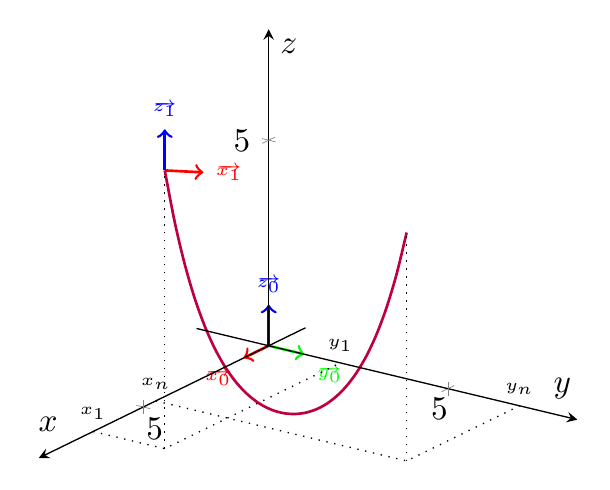
\begin{tikzpicture}[scale=1.2]
							\begin{axis}[view={125}{20},
								axis lines=center,axis on top,
								xlabel=$x$,ylabel=$y$,zlabel=$z$,
								no marks,axis equal,
								xmin=0,xmax=7,ymin=0,ymax=6,zmin=0,zmax=7,
								enlargelimits={upper=0.1}]
				
								% R0
								\draw[thick,->, red] (0,0,0) -- (1,0,0) node[anchor=north east] (x0) {\tiny $\overrightarrow{x_0}$};
								\draw[thick,->, green] (0,0,0) -- (0,1,0) node[anchor=north west] (y0) {\tiny $\overrightarrow{y_0}$};
								\draw[thick,->, blue] (0,0,0) -- (0,0,1) node[anchor=south] (z0) {\tiny $\overrightarrow{z_0}$};
				
								% R1
								\draw[thick,->, red] (7,2,6.769) -- ++(-0.4,0.8,0) node[anchor=west] (x1) {\tiny $\overrightarrow{x_1}$};
								\draw[thick,->, blue] (7,2,6.769) -- ++(0,0,1) node[anchor=south] (z1) {\tiny $\overrightarrow{z_1}$};
				
								% Tether
								\addplot3[
									samples y=0,
									smooth, thick, color=purple,
									domain=2:7
									] ({8-0.5*x},{x},{cosh(x-4.6)});
								
								% label points
								\node [above] at (7,0,0) {\tiny $x_1$};
								\node [above] at (0,2,0) {\tiny $y_1$};
								\node [above] at (4.5,0,0) {\tiny $x_n$};
								\node [above] at (0,7,0) {\tiny $y_n$};
				
								% Dots
								\draw[dotted] (7,0,0) -- (7,2,0) -- (0,2,0);
								\draw[dotted] (7,2,0) -- (7,2,6.769);
								
								\draw[dotted] (4.5,0,0) -- (4.5,7,0) -- (0,7,0);
								\draw[dotted] (4.5,7,0) -- (4.5,7,5.556);
							\end{axis}
						\end{tikzpicture}
						\caption{Dans le repère du monde}
						\label{fig:3d_plot}
					\end{subfigure}
					\hfill
					\begin{subfigure}[b]{0.45\textwidth}
						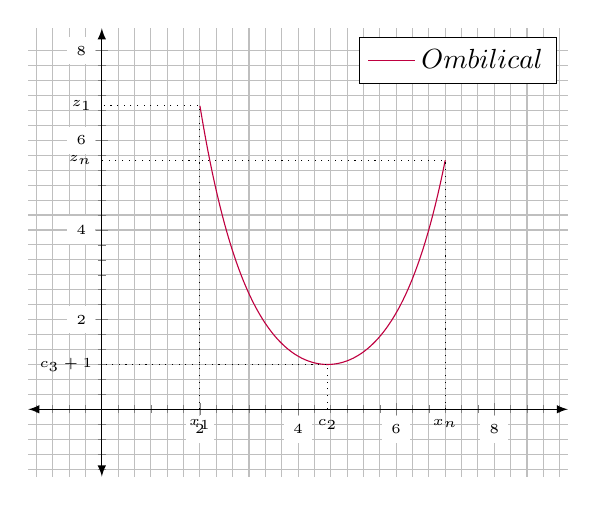
\begin{tikzpicture}
							\begin{axis}[
									xmin=-1,   xmax=9,
									ymin=-1,   ymax=8,
									grid=both,
									axis lines=middle,
									minor tick num=5,
									enlargelimits={abs=0.5},
									axis line style={latex-latex},
									ticklabel style={font=\tiny,fill=white},
									xlabel style={at={(ticklabel* cs:1)},anchor=north west},
									ylabel style={at={(ticklabel* cs:1)},anchor=south west}
								]
								\addplot [
									domain=2:7, 
									samples=100, 
									color=purple,
									]
									{cosh(\x - 4.6)};
								\addlegendentry{$Ombilical$}
			
								% Labels
								\node[below] at (2,0) {\tiny $x_1$};
								\node[below] at (7,0) {\tiny $x_n$};
								\node[left] at (0,6.769) {\tiny $z_1$};
								\node[left] at (0,5.556) {\tiny $z_n$};
								\node[left] at (0,1) {\tiny $c_3 + 1$};
								\node[below] at (4.6, 0) {\tiny $c_2$};
			
								% Dots
								\draw[dotted] (2,0) -- (2,6.769) -- (0,6.769);
								\draw[dotted] (4.6,0) -- (4.6,1) -- (0,1);
								\draw[dotted] (7,0) -- (7,5.556) -- (0,5.556);
							\end{axis}
						\end{tikzpicture}
						\caption{Dans le repère de l'ombilical}
						\label{fig:2d_plot}
					\end{subfigure}
					\caption{Modélisation de l'ombilical en 3 dimensions}
					\label{fig:tether_plot}
				\end{figure}
				
				Pour résoudre ce système et trouver une approximation numérique pour $c_1$, $c_2$ et $c_3$, on utilise un solveur numérique. Lors de l'implémentation pour le simulateur de cette étape d'initialisation, la librairie \textit{GSL}\footnote{\url{https://www.gnu.org/software/gsl/}} est utilisée. Une fois les paramètres déterminés, on est en mesure de déterminer la position initiale de chaque n\oe ud dans le repère de l'ombilical. Il faut enfin projeter ces positions dans le repère du monde afin de pouvoir correctement initialiser chaque n\oe uds, comme présenté sur la \textsc{Figure}~\ref{fig:tether_plot}
			
			\subsection{Couple transmissible}

				L'ombilical est capable de transmettre un couple longitudinal capable de traverser le câble et de se transmettre d'un bout à l'autre. Pour simuler ce couple, il va falloir ajouter une variable au vecteur d'état de chaque \textit{TetherElement}. Cette variable va contenir l'angle de chaque n\oe ud. Ensuite, un couple va être appliqué à chaque n\oe ud en fonction de son angle et de celui de son précédent voisin. Encore une fois, nous n'avons pas d'expression analytique pour ce couple, mais nous allons proposer un modèle comportemental permettant d'avoir un comportement physiquement acceptable.

				Le couple proposé peut être simplement un couple proportionnel à la différence d'angles entre l'élément courant et son élément précédent. Ici nous n'avons pas besoin de rejeter une erreur statique à l'aide d'un intégrateur dans la mesure où un ombilical réel peut encaisser un certain nombre de tours sur lui-même sans qu'il ne cherche à vouloir se dérouler complètement. Ainsi, en notant $K_c$ le coefficient permettant de gérer l'intensité de ce couple, $\theta_n$ l'angle de l'élément courant et $\theta_{n-1}$ l'angle de l'élément précédant, le couple ajouté au modèle s'exprime comme :

				\begin{equation}
					C = K_c \cdot (\theta_n - \theta_{n - 1})
				\end{equation}

				Le réglage de $K_c$ dépendra directement des caractéristiques mécaniques de l'ombilical et permettra de simuler des câbles avec plus ou moins de raideur vis-à-vis d'un couple transmissible le long de l'ombilical.
				
				Cependant, un problème survient avec la représentation numérique de l'orientation des solides. Celle-ci est souvent normalisée et les valeurs sont ainsi ramenées dans l'intervalle $[-\pi; \pi]$. On ne peut donc pas avoir l'orientation absolue, c’est-à-dire l'orientation d'un solide en prenant en compte les éventuels tours qu'il aurait pu faire sur lui-même et c'est le cas dans \gazebo{}.
			
				Pour résoudre ce problème, l'\textsc{Algorithme}~\ref{algo:suivi_angle} de suivi d'angles normalisés a été implémenté. Il prend en paramètres l'angle normalisé ainsi que l'angle précédemment calculé, et il retourne la valeur de l'angle absolu. En fournissant l'angle précédent on peut retourner le nouvel angle qui se trouve dans le même quadrant et ainsi de pouvoir suivre les sauts d'angles. On peut donc suivre l'orientation absolue de solides en rotation dans l'espace, en ne fournissant que des orientations relatives ramenées dans l'intervalle $[-\pi; \pi]$, et en gardant en mémoire la précédente orientation calculée.
				
				\begin{algorithm}[!htb]
					\SetKwInOut{Input}{Entrées}
					\SetKwInOut{Output}{Sorties}
					\Entree{$angle\_normalise$, $angle\_absolu$}
					\Sortie{$angle\_absolu$}
					\Deb{
						$offset \leftarrow (angle\_absolu - angle\_normalise + \pi ) \pmod{2\pi}$ \\
						$angle\_absolu \leftarrow angle\_normalise + 2\pi \cdot offset$ \\
					}
					\Retour{$angle\_absolu$}
			
					\caption{Suivi d'angle} 
					\label{algo:suivi_angle}
				\end{algorithm}
			
				La \textsc{Figure}~\ref{fig:suivi_angle} présente les résultats de l'\textsc{Algorithme}~\ref{algo:suivi_angle} avec un angle variant dans l'intervalle $[-3\pi; 3\pi]$. On voit sur la première sous-figure l'angle réel et l'angle ramené dans l'intervalle $[-\pi; \pi]$ avec la présence de saut d'angles. Avec cette méthode, on est capable de suivre l'évolution de l'angle et de supprimer ces sauts afin de retrouver l'angle absolu visible dans la deuxième sous-figure et calculé uniquement à partir de la connaissance de l'angle normalisé. Cet algorithme ne marche en revanche que pour une variation d'angle continue, car en cas de saut brusque d'angle les tours ajoutés ne seront pas pris en compte.
			
				\begin{figure}[!htb]
					\centering
					\includegraphics[]{build/imgs/absolute_orientation_tracking.pdf}
					\caption{Suivi d'angle}
					\label{fig:suivi_angle}
				\end{figure}		

			\subsection{Implémentation}

				L'implémentation d'un \plugin{} \gazebo{} permet de simuler le comportement de l'ombilical dans l'environnement de simulation. Ce \plugin{} est basé sur l'instanciation d'objets de type \textit{Tether} et \textit{TetherElement}. L'objet \textit{Tether} possède les paramètres de simulation de l'ombilical, tandis que l'objet \textit{TetherElement} représente un tronçon de cet ombilical. Un diagramme de classe est présenté en \textsc{Figure}~\ref{fig:uml_class} et montre les différents attributs et méthodes associées à chaque classe.
				est opéré
				\begin{figure}[!htb]
					\centering
					\resizebox{0.50\textwidth}{!}{
						\begin{tikzpicture}
							\begin{class}[text width=6cm]{Tether}{0,0}
								\attribute{+ element\_mass : double}
								\attribute{+ element\_volume : double}
								\attribute{+ element\_length : double}
								\attribute{+ position\_first : numpy.ndarray}
								\attribute{+ position\_last : numpy.ndarray}
								\attribute{+ elements : list of \textit{TetherElement}}
							\end{class}
						
							\begin{class}[text width=6cm]{TetherElement}{8.5,0}
								\attribute{+ mass : double}
								\attribute{+ volume : double}
								\attribute{+ length : double}
								\attribute{+ position : numpy.ndarray}
								\attribute{+ velocity : numpy.ndarray}
								\attribute{+ acceleration : numpy.ndarray}
								\attribute{+ previous : TetherElement}
								\attribute{+ next : TetherElement}
								\attribute{+ K\_p : double}
								\attribute{+ K\_d : double}
								\attribute{+ K\_i : double}
								\operation{+ F\_p(self) : numpy.ndarray}
								\operation{+ F\_b(self) : numpy.ndarray}
								\operation{+ F\_f(self) : numpy.ndarray}
								\operation{+ Ft\_prev(self) : numpy.ndarray}
								\operation{+ Ft\_next(self) : numpy.ndarray}
							\end{class}
						
							\aggregation{Tether}{}{~~~n}{TetherElement}
						\end{tikzpicture}
					}
					\caption{Diagramme de classe UML des classes \textit{Tether} et \textit{TetherElement}}
					\label{fig:uml_class}
				\end{figure}
				
				La \textit{Tether} utilise une structure de \textit{liste doublement chaînée}\footnote{structure de données liée qui consiste en un ensemble n\oe uds liés les uns aux autres par des références au n\oe uds voisins.} de \textit{TetherElement}. Chaque \textit{TetherElement} possède alors une référence vers l'élément le précédant et l'élément le suivant, comme le montre la \textsc{Figure}~\ref{fig:doubly_linked_list}. La \textit{Tether} ne possède ainsi qu'une référence vers le premier et le dernier n\oe ud de la chaîne, nommés respectivement \textit{head} et \textit{tail}. Il est ensuite possible de parcourir la chaîne de \textit{TetherElement} dans les deux sens en utilisant les références gardées par les \textit{TetherElement} eux-mêmes. 
			
				\begin{figure}[!htb]
					\centering
					\resizebox{0.90\textwidth}{!}{
						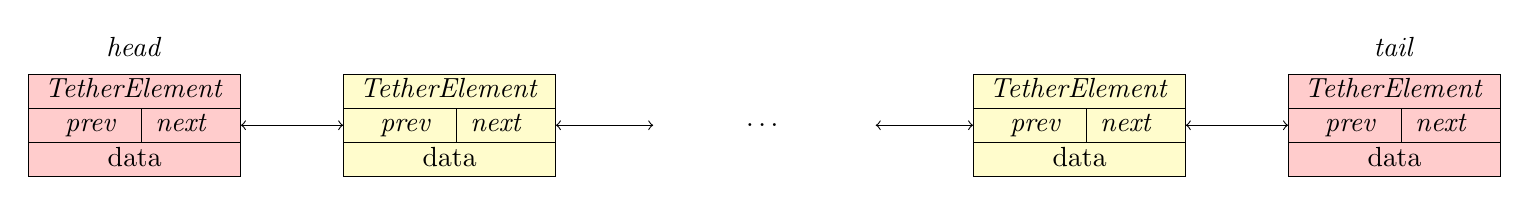
\begin{tikzpicture}
							\tikzset{TE/.style={draw, inner sep=0, outer sep=0, fill=yellow!20}}
			
							\node[TE, fill=red!20] (TE0) at (0,0) {\begin{tabular}{c} \textit{TetherElement} \\ \hline \hfill \textit{prev} \hfill \vline \hfill \textit{next} \hfill \\ \hline data \end{tabular}};
			
							\node[TE, fill=red!20] (TE4) at (16,0) {\begin{tabular}{c} \textit{TetherElement} \\ \hline \hfill \textit{prev} \hfill \vline \hfill \textit{next} \hfill \\ \hline data \end{tabular}};
			
							\foreach \i in {1,3} {
								\node[TE] (TE\i) at (4*\i,0) {\begin{tabular}{c} \textit{TetherElement} \\ \hline \hfill \textit{prev} \hfill \vline \hfill \textit{next} \hfill \\ \hline data \end{tabular}};
							}
							\node[minimum width=80] (TE2) at (8,0) {\dots};
							\foreach \i in {0,1,2,3} {
								\pgfmathtruncatemacro{\next}{\i +1}
								\draw[<->] (TE\i) -- (TE\next);
							}
			
							\node (head) at (0,1) {\textit{head}};
							\node (tail) at (16,1) {\textit{tail}};
						\end{tikzpicture}
					}
					\caption{Liste doublement chaînée}
					\label{fig:doubly_linked_list}
				\end{figure}

				A chaque pas de temps, on va actualiser la position des \textit{TetherElement}. Les extrémités peuvent être libres, dans ce cas on les traite comme les autres \textit{TetherElement}, ou bien attachée à des solides, dans ce cas la position actualisée est celle de l'élément auquel l'extrémité est attachée. Puis, on parcours la \textit{liste doublement chaînée} et on réalise le bilan des forces qui s'appliquent sur chaque élément. D'après le Principe Fondamental de la Dynamique, en notant $\overrightarrow{a}$ l'accélération d'un \textit{TetherElement}, on a :

				\begin{equation}
					m.\overrightarrow{a_{t_{i+1}}} = \overrightarrow{P} + \overrightarrow{\Pi} + \overrightarrow{F_f} + \overrightarrow{F_p} + \overrightarrow{F_s}
					\label{eq:newton}
				\end{equation}

				A ce stade, on peut appliquer l'accélération des \textit{TetherElement} aux extrémités dans les solides auxquels l'ombilical est attaché. Par exemple si l'ombilical simulé est attaché à un robot, il va induire une force à celui-ci qui va le gêner dans ses mouvements. Cette force est égale à l'opposé de la somme des forces calculées dans l'élément en extrémité d'ombilical.
				
				Ensuite, à l'aide de la méthode d'Euler on est en mesure d'obtenir une approximation de la vitesse puis de la position de chaque élément. En notant $\overrightarrow{v}$ la vitesse et $\overrightarrow{p}$ la position d'un \textit{TetherElement}, et $h$ le pas de temps entre deux instants de calculs, on a :

				\begin{eqnarray}
					\overrightarrow{v_{t_{i+1}}} & = & \overrightarrow{v_{t_i}} + h.\overrightarrow{a_{t_{i+1}}} \\
					\overrightarrow{p_{t_{i+1}}} & = & \overrightarrow{p_{t_i}} + h.\overrightarrow{v_{t_{i+1}}}
					\label{eq:euler}
				\end{eqnarray}

				On a donc actualisé la position de chaque \textit{TetherElement}. Après avoir actualisé la représentation graphique de cet élément dans \gazebo{}, on est prêt pour la prochaine itération de calcul.
			
		\subsection{Résultats}
			
			Le résultat de l'implémentation de l'ombilical est visible sur la \textsc{Figure}~\ref{fig:tether} dans l'environnement de simulation \gazebo{}. 
			
			\begin{figure}[!htb]
				\centering
				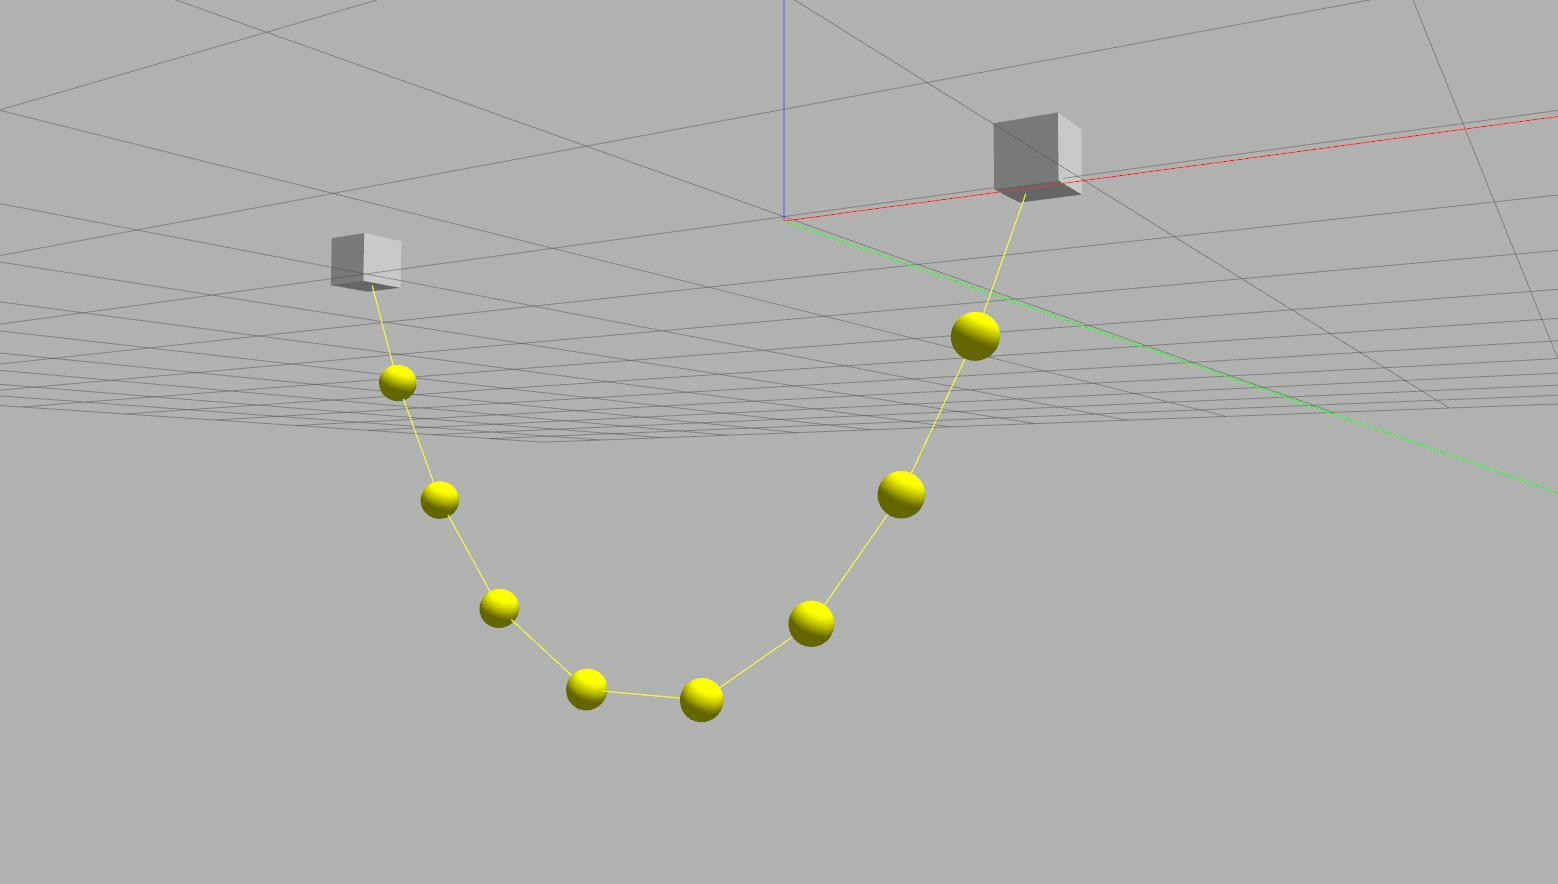
\includegraphics[width=0.8\textwidth]{imgs/tether_gazebo.png}
				\caption{Tether simulée avec 10 n\oe uds entre deux cubes}
				\label{fig:tether}
			\end{figure}
			
			L'ombilical est attaché à ses extrémités à deux cubes flottants et il prend bien une forme de chaînette afin de minimiser son énergie potentielle. Si l'on cherche à éloigner les cubes l'un de l'autre, l'ombilical va avoir tendence à les ramener du fait du poids qui s'applique sur lui, et une rotation d'un cube va avoir tendance à faire tourner l'autre sur lui-même du fait du couple transmissible le long de l'ombilical. Enfin, il est possible de dérouler l'ombilical en ajoutant des \textit{TetherElement} entre le premier et le deuxième n\oe ud, et de l'enrouler en supprimant le deuxième n\oe ud (car le premier est celui qui est fixé au cube). L'ombilical va réguler sa longueur avec les n\oe uds supplémentaires ou manquants et cela aura pour effet de pouvoir contôler la longueur de l'ombilical dans l'environnement de simulation.

			En traçant la distance entre chaque n\oe uds au cours du temps, on obtient la \textsc{Figure}~\ref{fig:length}. On se rend compte que le comportement de l'ombilical est consistant et que la longueur de chaque lien converge très vite vers la longueur consigne. Ainsi l'ombilical prends très vite la longueur consigne. 
			
			En traçant l'erreur relative de longueur de l'ombilical par rapport à la longueur consigne au cours du temps, on obtient la \textsc{Figure}~\ref{fig:error_length}. On voit sur cette figure que lors de l'initialisation, l'ombilical va s'étendre un peu avant de converger vers sa longueur consigne avec des légères oscillations. On remarque que l'initialisation à l'aide de l'équation de la chaînette a bien marché dans la mesure où l'erreur relative initiale de longueur est de $0 \%$. On peut expliquer le pic d'erreur relative par le fait que les n\oe uds sont soumis à une forte perturbation liée au poids, alors que la partie intégrale et dérivée du modèle comportemental des forces n'entre pas encore en jeu du fait de l'initialisation récente, mais qu'ils finissent bien par faire converger le système.

			\begin{figure}[!htb]
				\begin{subfigure}[t]{0.45\textwidth}
					\scalebox{0.8}{%% Creator: Matplotlib, PGF backend
%%
%% To include the figure in your LaTeX document, write
%%   \input{<filename>.pgf}
%%
%% Make sure the required packages are loaded in your preamble
%%   \usepackage{pgf}
%%
%% and, on pdftex
%%   \usepackage[utf8]{inputenc}\DeclareUnicodeCharacter{2212}{-}
%%
%% or, on luatex and xetex
%%   \usepackage{unicode-math}
%%
%% Figures using additional raster images can only be included by \input if
%% they are in the same directory as the main LaTeX file. For loading figures
%% from other directories you can use the `import` package
%%   \usepackage{import}
%%
%% and then include the figures with
%%   \import{<path to file>}{<filename>.pgf}
%%
%% Matplotlib used the following preamble
%%
\begingroup%
\makeatletter%
\begin{pgfpicture}%
\pgfpathrectangle{\pgfpointorigin}{\pgfqpoint{3.500000in}{2.800000in}}%
\pgfusepath{use as bounding box, clip}%
\begin{pgfscope}%
\pgfsetbuttcap%
\pgfsetmiterjoin%
\definecolor{currentfill}{rgb}{1.000000,1.000000,1.000000}%
\pgfsetfillcolor{currentfill}%
\pgfsetlinewidth{0.000000pt}%
\definecolor{currentstroke}{rgb}{1.000000,1.000000,1.000000}%
\pgfsetstrokecolor{currentstroke}%
\pgfsetdash{}{0pt}%
\pgfpathmoveto{\pgfqpoint{0.000000in}{0.000000in}}%
\pgfpathlineto{\pgfqpoint{3.500000in}{0.000000in}}%
\pgfpathlineto{\pgfqpoint{3.500000in}{2.800000in}}%
\pgfpathlineto{\pgfqpoint{0.000000in}{2.800000in}}%
\pgfpathclose%
\pgfusepath{fill}%
\end{pgfscope}%
\begin{pgfscope}%
\pgfsetbuttcap%
\pgfsetmiterjoin%
\definecolor{currentfill}{rgb}{1.000000,1.000000,1.000000}%
\pgfsetfillcolor{currentfill}%
\pgfsetlinewidth{0.000000pt}%
\definecolor{currentstroke}{rgb}{0.000000,0.000000,0.000000}%
\pgfsetstrokecolor{currentstroke}%
\pgfsetstrokeopacity{0.000000}%
\pgfsetdash{}{0pt}%
\pgfpathmoveto{\pgfqpoint{0.477013in}{0.523889in}}%
\pgfpathlineto{\pgfqpoint{3.300764in}{0.523889in}}%
\pgfpathlineto{\pgfqpoint{3.300764in}{2.665000in}}%
\pgfpathlineto{\pgfqpoint{0.477013in}{2.665000in}}%
\pgfpathclose%
\pgfusepath{fill}%
\end{pgfscope}%
\begin{pgfscope}%
\pgfpathrectangle{\pgfqpoint{0.477013in}{0.523889in}}{\pgfqpoint{2.823751in}{2.141111in}}%
\pgfusepath{clip}%
\pgfsetbuttcap%
\pgfsetroundjoin%
\definecolor{currentfill}{rgb}{0.000000,0.501961,0.501961}%
\pgfsetfillcolor{currentfill}%
\pgfsetfillopacity{0.400000}%
\pgfsetlinewidth{0.000000pt}%
\definecolor{currentstroke}{rgb}{0.000000,0.000000,0.000000}%
\pgfsetstrokecolor{currentstroke}%
\pgfsetdash{}{0pt}%
\pgfpathmoveto{\pgfqpoint{0.477013in}{2.567677in}}%
\pgfpathlineto{\pgfqpoint{0.477013in}{0.621212in}}%
\pgfpathlineto{\pgfqpoint{0.479837in}{0.621212in}}%
\pgfpathlineto{\pgfqpoint{0.482661in}{0.621212in}}%
\pgfpathlineto{\pgfqpoint{0.485485in}{0.621212in}}%
\pgfpathlineto{\pgfqpoint{0.488308in}{0.621212in}}%
\pgfpathlineto{\pgfqpoint{0.491132in}{0.621212in}}%
\pgfpathlineto{\pgfqpoint{0.493956in}{0.621212in}}%
\pgfpathlineto{\pgfqpoint{0.496780in}{0.621212in}}%
\pgfpathlineto{\pgfqpoint{0.499603in}{0.621212in}}%
\pgfpathlineto{\pgfqpoint{0.502427in}{0.621212in}}%
\pgfpathlineto{\pgfqpoint{0.505251in}{0.621212in}}%
\pgfpathlineto{\pgfqpoint{0.508075in}{0.621212in}}%
\pgfpathlineto{\pgfqpoint{0.510898in}{0.621212in}}%
\pgfpathlineto{\pgfqpoint{0.513722in}{0.681620in}}%
\pgfpathlineto{\pgfqpoint{0.516546in}{0.750254in}}%
\pgfpathlineto{\pgfqpoint{0.519370in}{0.815106in}}%
\pgfpathlineto{\pgfqpoint{0.522193in}{0.875375in}}%
\pgfpathlineto{\pgfqpoint{0.525017in}{0.930306in}}%
\pgfpathlineto{\pgfqpoint{0.527841in}{0.979310in}}%
\pgfpathlineto{\pgfqpoint{0.530665in}{1.022076in}}%
\pgfpathlineto{\pgfqpoint{0.533488in}{1.058637in}}%
\pgfpathlineto{\pgfqpoint{0.536312in}{1.089344in}}%
\pgfpathlineto{\pgfqpoint{0.539136in}{1.114747in}}%
\pgfpathlineto{\pgfqpoint{0.541960in}{1.135443in}}%
\pgfpathlineto{\pgfqpoint{0.544783in}{1.151964in}}%
\pgfpathlineto{\pgfqpoint{0.547607in}{1.164740in}}%
\pgfpathlineto{\pgfqpoint{0.550431in}{1.174130in}}%
\pgfpathlineto{\pgfqpoint{0.553255in}{1.180436in}}%
\pgfpathlineto{\pgfqpoint{0.556078in}{1.183920in}}%
\pgfpathlineto{\pgfqpoint{0.558902in}{1.184795in}}%
\pgfpathlineto{\pgfqpoint{0.561726in}{1.183242in}}%
\pgfpathlineto{\pgfqpoint{0.564550in}{1.179451in}}%
\pgfpathlineto{\pgfqpoint{0.567373in}{1.173652in}}%
\pgfpathlineto{\pgfqpoint{0.570197in}{1.166110in}}%
\pgfpathlineto{\pgfqpoint{0.573021in}{1.157118in}}%
\pgfpathlineto{\pgfqpoint{0.575845in}{1.146997in}}%
\pgfpathlineto{\pgfqpoint{0.578669in}{1.136120in}}%
\pgfpathlineto{\pgfqpoint{0.581492in}{1.124910in}}%
\pgfpathlineto{\pgfqpoint{0.584316in}{1.113833in}}%
\pgfpathlineto{\pgfqpoint{0.587140in}{1.103359in}}%
\pgfpathlineto{\pgfqpoint{0.589964in}{1.093919in}}%
\pgfpathlineto{\pgfqpoint{0.592787in}{1.085851in}}%
\pgfpathlineto{\pgfqpoint{0.595611in}{1.079358in}}%
\pgfpathlineto{\pgfqpoint{0.598435in}{1.074491in}}%
\pgfpathlineto{\pgfqpoint{0.601259in}{1.071162in}}%
\pgfpathlineto{\pgfqpoint{0.604082in}{1.069184in}}%
\pgfpathlineto{\pgfqpoint{0.606906in}{1.068319in}}%
\pgfpathlineto{\pgfqpoint{0.609730in}{1.068330in}}%
\pgfpathlineto{\pgfqpoint{0.612554in}{1.069007in}}%
\pgfpathlineto{\pgfqpoint{0.615377in}{1.070180in}}%
\pgfpathlineto{\pgfqpoint{0.618201in}{1.071702in}}%
\pgfpathlineto{\pgfqpoint{0.621025in}{1.073436in}}%
\pgfpathlineto{\pgfqpoint{0.623849in}{1.075237in}}%
\pgfpathlineto{\pgfqpoint{0.626672in}{1.076948in}}%
\pgfpathlineto{\pgfqpoint{0.629496in}{1.078408in}}%
\pgfpathlineto{\pgfqpoint{0.632320in}{1.079474in}}%
\pgfpathlineto{\pgfqpoint{0.635144in}{1.080048in}}%
\pgfpathlineto{\pgfqpoint{0.637967in}{1.080102in}}%
\pgfpathlineto{\pgfqpoint{0.640791in}{1.079698in}}%
\pgfpathlineto{\pgfqpoint{0.643615in}{1.078979in}}%
\pgfpathlineto{\pgfqpoint{0.646439in}{1.078146in}}%
\pgfpathlineto{\pgfqpoint{0.649262in}{1.077416in}}%
\pgfpathlineto{\pgfqpoint{0.652086in}{1.076982in}}%
\pgfpathlineto{\pgfqpoint{0.654910in}{1.076985in}}%
\pgfpathlineto{\pgfqpoint{0.657734in}{1.077492in}}%
\pgfpathlineto{\pgfqpoint{0.660557in}{1.078489in}}%
\pgfpathlineto{\pgfqpoint{0.663381in}{1.079896in}}%
\pgfpathlineto{\pgfqpoint{0.666205in}{1.081579in}}%
\pgfpathlineto{\pgfqpoint{0.669029in}{1.083361in}}%
\pgfpathlineto{\pgfqpoint{0.671852in}{1.085043in}}%
\pgfpathlineto{\pgfqpoint{0.674676in}{1.086409in}}%
\pgfpathlineto{\pgfqpoint{0.677500in}{1.087244in}}%
\pgfpathlineto{\pgfqpoint{0.680324in}{1.087344in}}%
\pgfpathlineto{\pgfqpoint{0.683147in}{1.086534in}}%
\pgfpathlineto{\pgfqpoint{0.685971in}{1.084685in}}%
\pgfpathlineto{\pgfqpoint{0.688795in}{1.081735in}}%
\pgfpathlineto{\pgfqpoint{0.691619in}{1.077698in}}%
\pgfpathlineto{\pgfqpoint{0.694442in}{1.072673in}}%
\pgfpathlineto{\pgfqpoint{0.697266in}{1.066845in}}%
\pgfpathlineto{\pgfqpoint{0.700090in}{1.060475in}}%
\pgfpathlineto{\pgfqpoint{0.702914in}{1.053873in}}%
\pgfpathlineto{\pgfqpoint{0.705737in}{1.047378in}}%
\pgfpathlineto{\pgfqpoint{0.708561in}{1.041330in}}%
\pgfpathlineto{\pgfqpoint{0.711385in}{1.036046in}}%
\pgfpathlineto{\pgfqpoint{0.714209in}{1.031795in}}%
\pgfpathlineto{\pgfqpoint{0.717032in}{1.028776in}}%
\pgfpathlineto{\pgfqpoint{0.719856in}{1.027101in}}%
\pgfpathlineto{\pgfqpoint{0.722680in}{1.026788in}}%
\pgfpathlineto{\pgfqpoint{0.725504in}{1.027764in}}%
\pgfpathlineto{\pgfqpoint{0.728327in}{1.029872in}}%
\pgfpathlineto{\pgfqpoint{0.731151in}{1.032896in}}%
\pgfpathlineto{\pgfqpoint{0.733975in}{1.036587in}}%
\pgfpathlineto{\pgfqpoint{0.736799in}{1.040687in}}%
\pgfpathlineto{\pgfqpoint{0.739622in}{1.044953in}}%
\pgfpathlineto{\pgfqpoint{0.742446in}{1.049173in}}%
\pgfpathlineto{\pgfqpoint{0.745270in}{1.053172in}}%
\pgfpathlineto{\pgfqpoint{0.748094in}{1.056823in}}%
\pgfpathlineto{\pgfqpoint{0.750917in}{1.060040in}}%
\pgfpathlineto{\pgfqpoint{0.753741in}{1.062790in}}%
\pgfpathlineto{\pgfqpoint{0.756565in}{1.065085in}}%
\pgfpathlineto{\pgfqpoint{0.759389in}{1.066982in}}%
\pgfpathlineto{\pgfqpoint{0.762212in}{1.068573in}}%
\pgfpathlineto{\pgfqpoint{0.765036in}{1.069965in}}%
\pgfpathlineto{\pgfqpoint{0.767860in}{1.071265in}}%
\pgfpathlineto{\pgfqpoint{0.770684in}{1.072560in}}%
\pgfpathlineto{\pgfqpoint{0.773507in}{1.073910in}}%
\pgfpathlineto{\pgfqpoint{0.776331in}{1.075341in}}%
\pgfpathlineto{\pgfqpoint{0.779155in}{1.076849in}}%
\pgfpathlineto{\pgfqpoint{0.781979in}{1.078406in}}%
\pgfpathlineto{\pgfqpoint{0.784802in}{1.079970in}}%
\pgfpathlineto{\pgfqpoint{0.787626in}{1.081491in}}%
\pgfpathlineto{\pgfqpoint{0.790450in}{1.082919in}}%
\pgfpathlineto{\pgfqpoint{0.793274in}{1.084204in}}%
\pgfpathlineto{\pgfqpoint{0.796097in}{1.085301in}}%
\pgfpathlineto{\pgfqpoint{0.798921in}{1.086169in}}%
\pgfpathlineto{\pgfqpoint{0.801745in}{1.086772in}}%
\pgfpathlineto{\pgfqpoint{0.804569in}{1.087081in}}%
\pgfpathlineto{\pgfqpoint{0.807392in}{1.087078in}}%
\pgfpathlineto{\pgfqpoint{0.810216in}{1.086753in}}%
\pgfpathlineto{\pgfqpoint{0.813040in}{1.086112in}}%
\pgfpathlineto{\pgfqpoint{0.815864in}{1.085176in}}%
\pgfpathlineto{\pgfqpoint{0.818687in}{1.083978in}}%
\pgfpathlineto{\pgfqpoint{0.821511in}{1.082568in}}%
\pgfpathlineto{\pgfqpoint{0.824335in}{1.081003in}}%
\pgfpathlineto{\pgfqpoint{0.827159in}{1.079351in}}%
\pgfpathlineto{\pgfqpoint{0.829982in}{1.077682in}}%
\pgfpathlineto{\pgfqpoint{0.832806in}{1.076064in}}%
\pgfpathlineto{\pgfqpoint{0.835630in}{1.074561in}}%
\pgfpathlineto{\pgfqpoint{0.838454in}{1.073230in}}%
\pgfpathlineto{\pgfqpoint{0.841277in}{1.072116in}}%
\pgfpathlineto{\pgfqpoint{0.844101in}{1.071252in}}%
\pgfpathlineto{\pgfqpoint{0.846925in}{1.070657in}}%
\pgfpathlineto{\pgfqpoint{0.849749in}{1.070339in}}%
\pgfpathlineto{\pgfqpoint{0.852572in}{1.070292in}}%
\pgfpathlineto{\pgfqpoint{0.855396in}{1.070498in}}%
\pgfpathlineto{\pgfqpoint{0.858220in}{1.070925in}}%
\pgfpathlineto{\pgfqpoint{0.861044in}{1.071531in}}%
\pgfpathlineto{\pgfqpoint{0.863867in}{1.072264in}}%
\pgfpathlineto{\pgfqpoint{0.866691in}{1.073065in}}%
\pgfpathlineto{\pgfqpoint{0.869515in}{1.073872in}}%
\pgfpathlineto{\pgfqpoint{0.872339in}{1.074626in}}%
\pgfpathlineto{\pgfqpoint{0.875162in}{1.075276in}}%
\pgfpathlineto{\pgfqpoint{0.877986in}{1.075783in}}%
\pgfpathlineto{\pgfqpoint{0.880810in}{1.076123in}}%
\pgfpathlineto{\pgfqpoint{0.883634in}{1.076289in}}%
\pgfpathlineto{\pgfqpoint{0.886457in}{1.076292in}}%
\pgfpathlineto{\pgfqpoint{0.889281in}{1.076153in}}%
\pgfpathlineto{\pgfqpoint{0.892105in}{1.075909in}}%
\pgfpathlineto{\pgfqpoint{0.894929in}{1.075600in}}%
\pgfpathlineto{\pgfqpoint{0.897752in}{1.075271in}}%
\pgfpathlineto{\pgfqpoint{0.900576in}{1.074967in}}%
\pgfpathlineto{\pgfqpoint{0.903400in}{1.074728in}}%
\pgfpathlineto{\pgfqpoint{0.906224in}{1.074592in}}%
\pgfpathlineto{\pgfqpoint{0.909047in}{1.074587in}}%
\pgfpathlineto{\pgfqpoint{0.911871in}{1.074734in}}%
\pgfpathlineto{\pgfqpoint{0.914695in}{1.075044in}}%
\pgfpathlineto{\pgfqpoint{0.917519in}{1.075516in}}%
\pgfpathlineto{\pgfqpoint{0.920342in}{1.076136in}}%
\pgfpathlineto{\pgfqpoint{0.923166in}{1.076884in}}%
\pgfpathlineto{\pgfqpoint{0.925990in}{1.077728in}}%
\pgfpathlineto{\pgfqpoint{0.928814in}{1.078630in}}%
\pgfpathlineto{\pgfqpoint{0.931637in}{1.079551in}}%
\pgfpathlineto{\pgfqpoint{0.934461in}{1.080457in}}%
\pgfpathlineto{\pgfqpoint{0.937285in}{1.081315in}}%
\pgfpathlineto{\pgfqpoint{0.940109in}{1.082106in}}%
\pgfpathlineto{\pgfqpoint{0.942932in}{1.082819in}}%
\pgfpathlineto{\pgfqpoint{0.945756in}{1.083457in}}%
\pgfpathlineto{\pgfqpoint{0.948580in}{1.084035in}}%
\pgfpathlineto{\pgfqpoint{0.951404in}{1.084577in}}%
\pgfpathlineto{\pgfqpoint{0.954227in}{1.085113in}}%
\pgfpathlineto{\pgfqpoint{0.957051in}{1.085676in}}%
\pgfpathlineto{\pgfqpoint{0.959875in}{1.086299in}}%
\pgfpathlineto{\pgfqpoint{0.962699in}{1.087013in}}%
\pgfpathlineto{\pgfqpoint{0.965522in}{1.087840in}}%
\pgfpathlineto{\pgfqpoint{0.968346in}{1.088798in}}%
\pgfpathlineto{\pgfqpoint{0.971170in}{1.089894in}}%
\pgfpathlineto{\pgfqpoint{0.973994in}{1.091126in}}%
\pgfpathlineto{\pgfqpoint{0.976817in}{1.092486in}}%
\pgfpathlineto{\pgfqpoint{0.979641in}{1.093956in}}%
\pgfpathlineto{\pgfqpoint{0.982465in}{1.095512in}}%
\pgfpathlineto{\pgfqpoint{0.985289in}{1.097122in}}%
\pgfpathlineto{\pgfqpoint{0.988112in}{1.098753in}}%
\pgfpathlineto{\pgfqpoint{0.990936in}{1.100365in}}%
\pgfpathlineto{\pgfqpoint{0.993760in}{1.101920in}}%
\pgfpathlineto{\pgfqpoint{0.996584in}{1.103380in}}%
\pgfpathlineto{\pgfqpoint{0.999407in}{1.104712in}}%
\pgfpathlineto{\pgfqpoint{1.002231in}{1.105887in}}%
\pgfpathlineto{\pgfqpoint{1.005055in}{1.106884in}}%
\pgfpathlineto{\pgfqpoint{1.007879in}{1.107691in}}%
\pgfpathlineto{\pgfqpoint{1.010702in}{1.108304in}}%
\pgfpathlineto{\pgfqpoint{1.013526in}{1.108727in}}%
\pgfpathlineto{\pgfqpoint{1.016350in}{1.108968in}}%
\pgfpathlineto{\pgfqpoint{1.019174in}{1.109044in}}%
\pgfpathlineto{\pgfqpoint{1.021997in}{1.108973in}}%
\pgfpathlineto{\pgfqpoint{1.024821in}{1.108779in}}%
\pgfpathlineto{\pgfqpoint{1.027645in}{1.108486in}}%
\pgfpathlineto{\pgfqpoint{1.030469in}{1.108120in}}%
\pgfpathlineto{\pgfqpoint{1.033292in}{1.107709in}}%
\pgfpathlineto{\pgfqpoint{1.036116in}{1.107278in}}%
\pgfpathlineto{\pgfqpoint{1.038940in}{1.106854in}}%
\pgfpathlineto{\pgfqpoint{1.041764in}{1.106458in}}%
\pgfpathlineto{\pgfqpoint{1.044587in}{1.106109in}}%
\pgfpathlineto{\pgfqpoint{1.047411in}{1.105821in}}%
\pgfpathlineto{\pgfqpoint{1.050235in}{1.105602in}}%
\pgfpathlineto{\pgfqpoint{1.053059in}{1.105454in}}%
\pgfpathlineto{\pgfqpoint{1.055882in}{1.105374in}}%
\pgfpathlineto{\pgfqpoint{1.058706in}{1.105354in}}%
\pgfpathlineto{\pgfqpoint{1.061530in}{1.105383in}}%
\pgfpathlineto{\pgfqpoint{1.064354in}{1.105451in}}%
\pgfpathlineto{\pgfqpoint{1.067177in}{1.105546in}}%
\pgfpathlineto{\pgfqpoint{1.070001in}{1.105660in}}%
\pgfpathlineto{\pgfqpoint{1.072825in}{1.105786in}}%
\pgfpathlineto{\pgfqpoint{1.075649in}{1.105920in}}%
\pgfpathlineto{\pgfqpoint{1.078472in}{1.106063in}}%
\pgfpathlineto{\pgfqpoint{1.081296in}{1.106215in}}%
\pgfpathlineto{\pgfqpoint{1.084120in}{1.106380in}}%
\pgfpathlineto{\pgfqpoint{1.086944in}{1.106562in}}%
\pgfpathlineto{\pgfqpoint{1.089767in}{1.106767in}}%
\pgfpathlineto{\pgfqpoint{1.092591in}{1.106998in}}%
\pgfpathlineto{\pgfqpoint{1.095415in}{1.107262in}}%
\pgfpathlineto{\pgfqpoint{1.098239in}{1.107563in}}%
\pgfpathlineto{\pgfqpoint{1.101062in}{1.107906in}}%
\pgfpathlineto{\pgfqpoint{1.103886in}{1.108292in}}%
\pgfpathlineto{\pgfqpoint{1.106710in}{1.108722in}}%
\pgfpathlineto{\pgfqpoint{1.109534in}{1.109195in}}%
\pgfpathlineto{\pgfqpoint{1.112357in}{1.109705in}}%
\pgfpathlineto{\pgfqpoint{1.115181in}{1.110244in}}%
\pgfpathlineto{\pgfqpoint{1.118005in}{1.110802in}}%
\pgfpathlineto{\pgfqpoint{1.120829in}{1.111367in}}%
\pgfpathlineto{\pgfqpoint{1.123652in}{1.111927in}}%
\pgfpathlineto{\pgfqpoint{1.126476in}{1.112473in}}%
\pgfpathlineto{\pgfqpoint{1.129300in}{1.112996in}}%
\pgfpathlineto{\pgfqpoint{1.132124in}{1.113492in}}%
\pgfpathlineto{\pgfqpoint{1.134947in}{1.113960in}}%
\pgfpathlineto{\pgfqpoint{1.137771in}{1.114406in}}%
\pgfpathlineto{\pgfqpoint{1.140595in}{1.114837in}}%
\pgfpathlineto{\pgfqpoint{1.143419in}{1.115265in}}%
\pgfpathlineto{\pgfqpoint{1.146242in}{1.115703in}}%
\pgfpathlineto{\pgfqpoint{1.149066in}{1.116167in}}%
\pgfpathlineto{\pgfqpoint{1.151890in}{1.116672in}}%
\pgfpathlineto{\pgfqpoint{1.154714in}{1.117234in}}%
\pgfpathlineto{\pgfqpoint{1.157537in}{1.117865in}}%
\pgfpathlineto{\pgfqpoint{1.160361in}{1.118578in}}%
\pgfpathlineto{\pgfqpoint{1.163185in}{1.119380in}}%
\pgfpathlineto{\pgfqpoint{1.166009in}{1.120274in}}%
\pgfpathlineto{\pgfqpoint{1.168832in}{1.121260in}}%
\pgfpathlineto{\pgfqpoint{1.171656in}{1.122331in}}%
\pgfpathlineto{\pgfqpoint{1.174480in}{1.123476in}}%
\pgfpathlineto{\pgfqpoint{1.177304in}{1.124679in}}%
\pgfpathlineto{\pgfqpoint{1.180127in}{1.125919in}}%
\pgfpathlineto{\pgfqpoint{1.182951in}{1.127174in}}%
\pgfpathlineto{\pgfqpoint{1.185775in}{1.128420in}}%
\pgfpathlineto{\pgfqpoint{1.188599in}{1.129631in}}%
\pgfpathlineto{\pgfqpoint{1.191422in}{1.130787in}}%
\pgfpathlineto{\pgfqpoint{1.194246in}{1.131865in}}%
\pgfpathlineto{\pgfqpoint{1.197070in}{1.132851in}}%
\pgfpathlineto{\pgfqpoint{1.199894in}{1.133731in}}%
\pgfpathlineto{\pgfqpoint{1.202717in}{1.134497in}}%
\pgfpathlineto{\pgfqpoint{1.205541in}{1.135144in}}%
\pgfpathlineto{\pgfqpoint{1.208365in}{1.135672in}}%
\pgfpathlineto{\pgfqpoint{1.211189in}{1.136082in}}%
\pgfpathlineto{\pgfqpoint{1.214012in}{1.136377in}}%
\pgfpathlineto{\pgfqpoint{1.216836in}{1.136564in}}%
\pgfpathlineto{\pgfqpoint{1.219660in}{1.136650in}}%
\pgfpathlineto{\pgfqpoint{1.222484in}{1.136643in}}%
\pgfpathlineto{\pgfqpoint{1.225307in}{1.136552in}}%
\pgfpathlineto{\pgfqpoint{1.228131in}{1.136387in}}%
\pgfpathlineto{\pgfqpoint{1.230955in}{1.136158in}}%
\pgfpathlineto{\pgfqpoint{1.233779in}{1.135875in}}%
\pgfpathlineto{\pgfqpoint{1.236602in}{1.135547in}}%
\pgfpathlineto{\pgfqpoint{1.239426in}{1.135183in}}%
\pgfpathlineto{\pgfqpoint{1.242250in}{1.134790in}}%
\pgfpathlineto{\pgfqpoint{1.245074in}{1.134377in}}%
\pgfpathlineto{\pgfqpoint{1.247897in}{1.133951in}}%
\pgfpathlineto{\pgfqpoint{1.250721in}{1.133520in}}%
\pgfpathlineto{\pgfqpoint{1.253545in}{1.133092in}}%
\pgfpathlineto{\pgfqpoint{1.256369in}{1.132674in}}%
\pgfpathlineto{\pgfqpoint{1.259192in}{1.132274in}}%
\pgfpathlineto{\pgfqpoint{1.262016in}{1.131900in}}%
\pgfpathlineto{\pgfqpoint{1.264840in}{1.131558in}}%
\pgfpathlineto{\pgfqpoint{1.267664in}{1.131256in}}%
\pgfpathlineto{\pgfqpoint{1.270487in}{1.130998in}}%
\pgfpathlineto{\pgfqpoint{1.273311in}{1.130789in}}%
\pgfpathlineto{\pgfqpoint{1.276135in}{1.130633in}}%
\pgfpathlineto{\pgfqpoint{1.278959in}{1.130533in}}%
\pgfpathlineto{\pgfqpoint{1.281782in}{1.130494in}}%
\pgfpathlineto{\pgfqpoint{1.284606in}{1.130517in}}%
\pgfpathlineto{\pgfqpoint{1.287430in}{1.130607in}}%
\pgfpathlineto{\pgfqpoint{1.290254in}{1.130765in}}%
\pgfpathlineto{\pgfqpoint{1.293077in}{1.130991in}}%
\pgfpathlineto{\pgfqpoint{1.295901in}{1.131286in}}%
\pgfpathlineto{\pgfqpoint{1.298725in}{1.131645in}}%
\pgfpathlineto{\pgfqpoint{1.301549in}{1.132062in}}%
\pgfpathlineto{\pgfqpoint{1.304372in}{1.132531in}}%
\pgfpathlineto{\pgfqpoint{1.307196in}{1.133041in}}%
\pgfpathlineto{\pgfqpoint{1.310020in}{1.133579in}}%
\pgfpathlineto{\pgfqpoint{1.312844in}{1.134134in}}%
\pgfpathlineto{\pgfqpoint{1.315667in}{1.134694in}}%
\pgfpathlineto{\pgfqpoint{1.318491in}{1.135249in}}%
\pgfpathlineto{\pgfqpoint{1.321315in}{1.135789in}}%
\pgfpathlineto{\pgfqpoint{1.324139in}{1.136310in}}%
\pgfpathlineto{\pgfqpoint{1.326962in}{1.136809in}}%
\pgfpathlineto{\pgfqpoint{1.329786in}{1.137288in}}%
\pgfpathlineto{\pgfqpoint{1.332610in}{1.137751in}}%
\pgfpathlineto{\pgfqpoint{1.335434in}{1.138207in}}%
\pgfpathlineto{\pgfqpoint{1.338257in}{1.138665in}}%
\pgfpathlineto{\pgfqpoint{1.341081in}{1.139138in}}%
\pgfpathlineto{\pgfqpoint{1.343905in}{1.139642in}}%
\pgfpathlineto{\pgfqpoint{1.346729in}{1.140190in}}%
\pgfpathlineto{\pgfqpoint{1.349552in}{1.140795in}}%
\pgfpathlineto{\pgfqpoint{1.352376in}{1.141468in}}%
\pgfpathlineto{\pgfqpoint{1.355200in}{1.142215in}}%
\pgfpathlineto{\pgfqpoint{1.358024in}{1.143038in}}%
\pgfpathlineto{\pgfqpoint{1.360847in}{1.143933in}}%
\pgfpathlineto{\pgfqpoint{1.363671in}{1.144891in}}%
\pgfpathlineto{\pgfqpoint{1.366495in}{1.145895in}}%
\pgfpathlineto{\pgfqpoint{1.369319in}{1.146928in}}%
\pgfpathlineto{\pgfqpoint{1.372142in}{1.147969in}}%
\pgfpathlineto{\pgfqpoint{1.374966in}{1.148996in}}%
\pgfpathlineto{\pgfqpoint{1.377790in}{1.149986in}}%
\pgfpathlineto{\pgfqpoint{1.380614in}{1.150923in}}%
\pgfpathlineto{\pgfqpoint{1.383437in}{1.151789in}}%
\pgfpathlineto{\pgfqpoint{1.386261in}{1.152572in}}%
\pgfpathlineto{\pgfqpoint{1.389085in}{1.153264in}}%
\pgfpathlineto{\pgfqpoint{1.391909in}{1.153857in}}%
\pgfpathlineto{\pgfqpoint{1.394732in}{1.154350in}}%
\pgfpathlineto{\pgfqpoint{1.397556in}{1.154741in}}%
\pgfpathlineto{\pgfqpoint{1.400380in}{1.155031in}}%
\pgfpathlineto{\pgfqpoint{1.403204in}{1.155223in}}%
\pgfpathlineto{\pgfqpoint{1.406027in}{1.155321in}}%
\pgfpathlineto{\pgfqpoint{1.408851in}{1.155329in}}%
\pgfpathlineto{\pgfqpoint{1.411675in}{1.155252in}}%
\pgfpathlineto{\pgfqpoint{1.414499in}{1.155096in}}%
\pgfpathlineto{\pgfqpoint{1.417322in}{1.154866in}}%
\pgfpathlineto{\pgfqpoint{1.420146in}{1.154565in}}%
\pgfpathlineto{\pgfqpoint{1.422970in}{1.154198in}}%
\pgfpathlineto{\pgfqpoint{1.425794in}{1.153767in}}%
\pgfpathlineto{\pgfqpoint{1.428618in}{1.153277in}}%
\pgfpathlineto{\pgfqpoint{1.431441in}{1.152731in}}%
\pgfpathlineto{\pgfqpoint{1.434265in}{1.152137in}}%
\pgfpathlineto{\pgfqpoint{1.437089in}{1.151499in}}%
\pgfpathlineto{\pgfqpoint{1.439913in}{1.150827in}}%
\pgfpathlineto{\pgfqpoint{1.442736in}{1.150129in}}%
\pgfpathlineto{\pgfqpoint{1.445560in}{1.149415in}}%
\pgfpathlineto{\pgfqpoint{1.448384in}{1.148696in}}%
\pgfpathlineto{\pgfqpoint{1.451208in}{1.147983in}}%
\pgfpathlineto{\pgfqpoint{1.454031in}{1.147284in}}%
\pgfpathlineto{\pgfqpoint{1.456855in}{1.146612in}}%
\pgfpathlineto{\pgfqpoint{1.459679in}{1.145976in}}%
\pgfpathlineto{\pgfqpoint{1.462503in}{1.145387in}}%
\pgfpathlineto{\pgfqpoint{1.465326in}{1.144855in}}%
\pgfpathlineto{\pgfqpoint{1.468150in}{1.144392in}}%
\pgfpathlineto{\pgfqpoint{1.470974in}{1.144009in}}%
\pgfpathlineto{\pgfqpoint{1.473798in}{1.143718in}}%
\pgfpathlineto{\pgfqpoint{1.476621in}{1.143526in}}%
\pgfpathlineto{\pgfqpoint{1.479445in}{1.143443in}}%
\pgfpathlineto{\pgfqpoint{1.482269in}{1.143471in}}%
\pgfpathlineto{\pgfqpoint{1.485093in}{1.143613in}}%
\pgfpathlineto{\pgfqpoint{1.487916in}{1.143864in}}%
\pgfpathlineto{\pgfqpoint{1.490740in}{1.144217in}}%
\pgfpathlineto{\pgfqpoint{1.493564in}{1.144664in}}%
\pgfpathlineto{\pgfqpoint{1.496388in}{1.145193in}}%
\pgfpathlineto{\pgfqpoint{1.499211in}{1.145790in}}%
\pgfpathlineto{\pgfqpoint{1.502035in}{1.146441in}}%
\pgfpathlineto{\pgfqpoint{1.504859in}{1.147134in}}%
\pgfpathlineto{\pgfqpoint{1.507683in}{1.147856in}}%
\pgfpathlineto{\pgfqpoint{1.510506in}{1.148597in}}%
\pgfpathlineto{\pgfqpoint{1.513330in}{1.149349in}}%
\pgfpathlineto{\pgfqpoint{1.516154in}{1.150105in}}%
\pgfpathlineto{\pgfqpoint{1.518978in}{1.150864in}}%
\pgfpathlineto{\pgfqpoint{1.521801in}{1.151627in}}%
\pgfpathlineto{\pgfqpoint{1.524625in}{1.152397in}}%
\pgfpathlineto{\pgfqpoint{1.527449in}{1.153180in}}%
\pgfpathlineto{\pgfqpoint{1.530273in}{1.153986in}}%
\pgfpathlineto{\pgfqpoint{1.533096in}{1.154822in}}%
\pgfpathlineto{\pgfqpoint{1.535920in}{1.155699in}}%
\pgfpathlineto{\pgfqpoint{1.538744in}{1.156620in}}%
\pgfpathlineto{\pgfqpoint{1.541568in}{1.157589in}}%
\pgfpathlineto{\pgfqpoint{1.544391in}{1.158603in}}%
\pgfpathlineto{\pgfqpoint{1.547215in}{1.159652in}}%
\pgfpathlineto{\pgfqpoint{1.550039in}{1.160724in}}%
\pgfpathlineto{\pgfqpoint{1.552863in}{1.161799in}}%
\pgfpathlineto{\pgfqpoint{1.555686in}{1.162858in}}%
\pgfpathlineto{\pgfqpoint{1.558510in}{1.163878in}}%
\pgfpathlineto{\pgfqpoint{1.561334in}{1.164837in}}%
\pgfpathlineto{\pgfqpoint{1.564158in}{1.165717in}}%
\pgfpathlineto{\pgfqpoint{1.566981in}{1.166503in}}%
\pgfpathlineto{\pgfqpoint{1.569805in}{1.167185in}}%
\pgfpathlineto{\pgfqpoint{1.572629in}{1.167755in}}%
\pgfpathlineto{\pgfqpoint{1.575453in}{1.168211in}}%
\pgfpathlineto{\pgfqpoint{1.578276in}{1.168552in}}%
\pgfpathlineto{\pgfqpoint{1.581100in}{1.168779in}}%
\pgfpathlineto{\pgfqpoint{1.583924in}{1.168896in}}%
\pgfpathlineto{\pgfqpoint{1.586748in}{1.168907in}}%
\pgfpathlineto{\pgfqpoint{1.589571in}{1.168818in}}%
\pgfpathlineto{\pgfqpoint{1.592395in}{1.168635in}}%
\pgfpathlineto{\pgfqpoint{1.595219in}{1.168364in}}%
\pgfpathlineto{\pgfqpoint{1.598043in}{1.168012in}}%
\pgfpathlineto{\pgfqpoint{1.600866in}{1.167584in}}%
\pgfpathlineto{\pgfqpoint{1.603690in}{1.167084in}}%
\pgfpathlineto{\pgfqpoint{1.606514in}{1.166515in}}%
\pgfpathlineto{\pgfqpoint{1.609338in}{1.165880in}}%
\pgfpathlineto{\pgfqpoint{1.612161in}{1.165181in}}%
\pgfpathlineto{\pgfqpoint{1.614985in}{1.164421in}}%
\pgfpathlineto{\pgfqpoint{1.617809in}{1.163606in}}%
\pgfpathlineto{\pgfqpoint{1.620633in}{1.162744in}}%
\pgfpathlineto{\pgfqpoint{1.623456in}{1.161845in}}%
\pgfpathlineto{\pgfqpoint{1.626280in}{1.160920in}}%
\pgfpathlineto{\pgfqpoint{1.629104in}{1.159980in}}%
\pgfpathlineto{\pgfqpoint{1.631928in}{1.159034in}}%
\pgfpathlineto{\pgfqpoint{1.634751in}{1.158091in}}%
\pgfpathlineto{\pgfqpoint{1.637575in}{1.157159in}}%
\pgfpathlineto{\pgfqpoint{1.640399in}{1.156244in}}%
\pgfpathlineto{\pgfqpoint{1.643223in}{1.155350in}}%
\pgfpathlineto{\pgfqpoint{1.646046in}{1.154487in}}%
\pgfpathlineto{\pgfqpoint{1.648870in}{1.153661in}}%
\pgfpathlineto{\pgfqpoint{1.651694in}{1.152886in}}%
\pgfpathlineto{\pgfqpoint{1.654518in}{1.152176in}}%
\pgfpathlineto{\pgfqpoint{1.657341in}{1.151546in}}%
\pgfpathlineto{\pgfqpoint{1.660165in}{1.151012in}}%
\pgfpathlineto{\pgfqpoint{1.662989in}{1.150590in}}%
\pgfpathlineto{\pgfqpoint{1.665813in}{1.150290in}}%
\pgfpathlineto{\pgfqpoint{1.668636in}{1.150121in}}%
\pgfpathlineto{\pgfqpoint{1.671460in}{1.150086in}}%
\pgfpathlineto{\pgfqpoint{1.674284in}{1.150184in}}%
\pgfpathlineto{\pgfqpoint{1.677108in}{1.150408in}}%
\pgfpathlineto{\pgfqpoint{1.679931in}{1.150749in}}%
\pgfpathlineto{\pgfqpoint{1.682755in}{1.151195in}}%
\pgfpathlineto{\pgfqpoint{1.685579in}{1.151734in}}%
\pgfpathlineto{\pgfqpoint{1.688403in}{1.152352in}}%
\pgfpathlineto{\pgfqpoint{1.691226in}{1.153036in}}%
\pgfpathlineto{\pgfqpoint{1.694050in}{1.153775in}}%
\pgfpathlineto{\pgfqpoint{1.696874in}{1.154556in}}%
\pgfpathlineto{\pgfqpoint{1.699698in}{1.155373in}}%
\pgfpathlineto{\pgfqpoint{1.702521in}{1.156217in}}%
\pgfpathlineto{\pgfqpoint{1.705345in}{1.157087in}}%
\pgfpathlineto{\pgfqpoint{1.708169in}{1.157981in}}%
\pgfpathlineto{\pgfqpoint{1.710993in}{1.158903in}}%
\pgfpathlineto{\pgfqpoint{1.713816in}{1.159857in}}%
\pgfpathlineto{\pgfqpoint{1.716640in}{1.160851in}}%
\pgfpathlineto{\pgfqpoint{1.719464in}{1.161892in}}%
\pgfpathlineto{\pgfqpoint{1.722288in}{1.162985in}}%
\pgfpathlineto{\pgfqpoint{1.725111in}{1.164130in}}%
\pgfpathlineto{\pgfqpoint{1.727935in}{1.165321in}}%
\pgfpathlineto{\pgfqpoint{1.730759in}{1.166544in}}%
\pgfpathlineto{\pgfqpoint{1.733583in}{1.167779in}}%
\pgfpathlineto{\pgfqpoint{1.736406in}{1.168996in}}%
\pgfpathlineto{\pgfqpoint{1.739230in}{1.170166in}}%
\pgfpathlineto{\pgfqpoint{1.742054in}{1.171257in}}%
\pgfpathlineto{\pgfqpoint{1.744878in}{1.172242in}}%
\pgfpathlineto{\pgfqpoint{1.747701in}{1.173103in}}%
\pgfpathlineto{\pgfqpoint{1.750525in}{1.173830in}}%
\pgfpathlineto{\pgfqpoint{1.753349in}{1.174425in}}%
\pgfpathlineto{\pgfqpoint{1.756173in}{1.174893in}}%
\pgfpathlineto{\pgfqpoint{1.758996in}{1.175249in}}%
\pgfpathlineto{\pgfqpoint{1.761820in}{1.175503in}}%
\pgfpathlineto{\pgfqpoint{1.764644in}{1.175665in}}%
\pgfpathlineto{\pgfqpoint{1.767468in}{1.175741in}}%
\pgfpathlineto{\pgfqpoint{1.770291in}{1.175729in}}%
\pgfpathlineto{\pgfqpoint{1.773115in}{1.175629in}}%
\pgfpathlineto{\pgfqpoint{1.775939in}{1.175434in}}%
\pgfpathlineto{\pgfqpoint{1.778763in}{1.175143in}}%
\pgfpathlineto{\pgfqpoint{1.781586in}{1.174753in}}%
\pgfpathlineto{\pgfqpoint{1.784410in}{1.174267in}}%
\pgfpathlineto{\pgfqpoint{1.787234in}{1.173688in}}%
\pgfpathlineto{\pgfqpoint{1.790058in}{1.173022in}}%
\pgfpathlineto{\pgfqpoint{1.792881in}{1.172277in}}%
\pgfpathlineto{\pgfqpoint{1.795705in}{1.171460in}}%
\pgfpathlineto{\pgfqpoint{1.798529in}{1.170583in}}%
\pgfpathlineto{\pgfqpoint{1.801353in}{1.169658in}}%
\pgfpathlineto{\pgfqpoint{1.804176in}{1.168697in}}%
\pgfpathlineto{\pgfqpoint{1.807000in}{1.167717in}}%
\pgfpathlineto{\pgfqpoint{1.809824in}{1.166731in}}%
\pgfpathlineto{\pgfqpoint{1.812648in}{1.165751in}}%
\pgfpathlineto{\pgfqpoint{1.815471in}{1.164787in}}%
\pgfpathlineto{\pgfqpoint{1.818295in}{1.163842in}}%
\pgfpathlineto{\pgfqpoint{1.821119in}{1.162915in}}%
\pgfpathlineto{\pgfqpoint{1.823943in}{1.162000in}}%
\pgfpathlineto{\pgfqpoint{1.826766in}{1.161091in}}%
\pgfpathlineto{\pgfqpoint{1.829590in}{1.160182in}}%
\pgfpathlineto{\pgfqpoint{1.832414in}{1.159274in}}%
\pgfpathlineto{\pgfqpoint{1.835238in}{1.158375in}}%
\pgfpathlineto{\pgfqpoint{1.838061in}{1.157500in}}%
\pgfpathlineto{\pgfqpoint{1.840885in}{1.156672in}}%
\pgfpathlineto{\pgfqpoint{1.843709in}{1.155918in}}%
\pgfpathlineto{\pgfqpoint{1.846533in}{1.155266in}}%
\pgfpathlineto{\pgfqpoint{1.849356in}{1.154741in}}%
\pgfpathlineto{\pgfqpoint{1.852180in}{1.154364in}}%
\pgfpathlineto{\pgfqpoint{1.855004in}{1.154147in}}%
\pgfpathlineto{\pgfqpoint{1.857828in}{1.154095in}}%
\pgfpathlineto{\pgfqpoint{1.860651in}{1.154206in}}%
\pgfpathlineto{\pgfqpoint{1.863475in}{1.154472in}}%
\pgfpathlineto{\pgfqpoint{1.866299in}{1.154881in}}%
\pgfpathlineto{\pgfqpoint{1.869123in}{1.155419in}}%
\pgfpathlineto{\pgfqpoint{1.871946in}{1.156069in}}%
\pgfpathlineto{\pgfqpoint{1.874770in}{1.156815in}}%
\pgfpathlineto{\pgfqpoint{1.877594in}{1.157641in}}%
\pgfpathlineto{\pgfqpoint{1.880418in}{1.158532in}}%
\pgfpathlineto{\pgfqpoint{1.883241in}{1.159472in}}%
\pgfpathlineto{\pgfqpoint{1.886065in}{1.160449in}}%
\pgfpathlineto{\pgfqpoint{1.888889in}{1.161452in}}%
\pgfpathlineto{\pgfqpoint{1.891713in}{1.162475in}}%
\pgfpathlineto{\pgfqpoint{1.894536in}{1.163516in}}%
\pgfpathlineto{\pgfqpoint{1.897360in}{1.164577in}}%
\pgfpathlineto{\pgfqpoint{1.900184in}{1.165664in}}%
\pgfpathlineto{\pgfqpoint{1.903008in}{1.166787in}}%
\pgfpathlineto{\pgfqpoint{1.905831in}{1.167953in}}%
\pgfpathlineto{\pgfqpoint{1.908655in}{1.169166in}}%
\pgfpathlineto{\pgfqpoint{1.911479in}{1.170423in}}%
\pgfpathlineto{\pgfqpoint{1.914303in}{1.171707in}}%
\pgfpathlineto{\pgfqpoint{1.917126in}{1.172989in}}%
\pgfpathlineto{\pgfqpoint{1.919950in}{1.174230in}}%
\pgfpathlineto{\pgfqpoint{1.922774in}{1.175381in}}%
\pgfpathlineto{\pgfqpoint{1.925598in}{1.176395in}}%
\pgfpathlineto{\pgfqpoint{1.928421in}{1.177234in}}%
\pgfpathlineto{\pgfqpoint{1.931245in}{1.177877in}}%
\pgfpathlineto{\pgfqpoint{1.934069in}{1.178328in}}%
\pgfpathlineto{\pgfqpoint{1.936893in}{1.178609in}}%
\pgfpathlineto{\pgfqpoint{1.939716in}{1.178755in}}%
\pgfpathlineto{\pgfqpoint{1.942540in}{1.178805in}}%
\pgfpathlineto{\pgfqpoint{1.945364in}{1.178790in}}%
\pgfpathlineto{\pgfqpoint{1.948188in}{1.178732in}}%
\pgfpathlineto{\pgfqpoint{1.951011in}{1.178640in}}%
\pgfpathlineto{\pgfqpoint{1.953835in}{1.178513in}}%
\pgfpathlineto{\pgfqpoint{1.956659in}{1.178347in}}%
\pgfpathlineto{\pgfqpoint{1.959483in}{1.178133in}}%
\pgfpathlineto{\pgfqpoint{1.962306in}{1.177862in}}%
\pgfpathlineto{\pgfqpoint{1.965130in}{1.177528in}}%
\pgfpathlineto{\pgfqpoint{1.967954in}{1.177126in}}%
\pgfpathlineto{\pgfqpoint{1.970778in}{1.176652in}}%
\pgfpathlineto{\pgfqpoint{1.973601in}{1.176107in}}%
\pgfpathlineto{\pgfqpoint{1.976425in}{1.175490in}}%
\pgfpathlineto{\pgfqpoint{1.979249in}{1.174808in}}%
\pgfpathlineto{\pgfqpoint{1.982073in}{1.174069in}}%
\pgfpathlineto{\pgfqpoint{1.984896in}{1.173285in}}%
\pgfpathlineto{\pgfqpoint{1.987720in}{1.172468in}}%
\pgfpathlineto{\pgfqpoint{1.990544in}{1.171632in}}%
\pgfpathlineto{\pgfqpoint{1.993368in}{1.170789in}}%
\pgfpathlineto{\pgfqpoint{1.996191in}{1.169947in}}%
\pgfpathlineto{\pgfqpoint{1.999015in}{1.169110in}}%
\pgfpathlineto{\pgfqpoint{2.001839in}{1.168273in}}%
\pgfpathlineto{\pgfqpoint{2.004663in}{1.167431in}}%
\pgfpathlineto{\pgfqpoint{2.007486in}{1.166572in}}%
\pgfpathlineto{\pgfqpoint{2.010310in}{1.165684in}}%
\pgfpathlineto{\pgfqpoint{2.013134in}{1.164759in}}%
\pgfpathlineto{\pgfqpoint{2.015958in}{1.163797in}}%
\pgfpathlineto{\pgfqpoint{2.018781in}{1.162804in}}%
\pgfpathlineto{\pgfqpoint{2.021605in}{1.161802in}}%
\pgfpathlineto{\pgfqpoint{2.024429in}{1.160819in}}%
\pgfpathlineto{\pgfqpoint{2.027253in}{1.159893in}}%
\pgfpathlineto{\pgfqpoint{2.030076in}{1.159064in}}%
\pgfpathlineto{\pgfqpoint{2.032900in}{1.158368in}}%
\pgfpathlineto{\pgfqpoint{2.035724in}{1.157835in}}%
\pgfpathlineto{\pgfqpoint{2.038548in}{1.157484in}}%
\pgfpathlineto{\pgfqpoint{2.041371in}{1.157319in}}%
\pgfpathlineto{\pgfqpoint{2.044195in}{1.157337in}}%
\pgfpathlineto{\pgfqpoint{2.047019in}{1.157526in}}%
\pgfpathlineto{\pgfqpoint{2.049843in}{1.157867in}}%
\pgfpathlineto{\pgfqpoint{2.052666in}{1.158342in}}%
\pgfpathlineto{\pgfqpoint{2.055490in}{1.158937in}}%
\pgfpathlineto{\pgfqpoint{2.058314in}{1.159638in}}%
\pgfpathlineto{\pgfqpoint{2.061138in}{1.160434in}}%
\pgfpathlineto{\pgfqpoint{2.063961in}{1.161312in}}%
\pgfpathlineto{\pgfqpoint{2.066785in}{1.162261in}}%
\pgfpathlineto{\pgfqpoint{2.069609in}{1.163264in}}%
\pgfpathlineto{\pgfqpoint{2.072433in}{1.164306in}}%
\pgfpathlineto{\pgfqpoint{2.075256in}{1.165370in}}%
\pgfpathlineto{\pgfqpoint{2.078080in}{1.166446in}}%
\pgfpathlineto{\pgfqpoint{2.080904in}{1.167530in}}%
\pgfpathlineto{\pgfqpoint{2.083728in}{1.168624in}}%
\pgfpathlineto{\pgfqpoint{2.086551in}{1.169735in}}%
\pgfpathlineto{\pgfqpoint{2.089375in}{1.170869in}}%
\pgfpathlineto{\pgfqpoint{2.092199in}{1.172027in}}%
\pgfpathlineto{\pgfqpoint{2.095023in}{1.173198in}}%
\pgfpathlineto{\pgfqpoint{2.097846in}{1.174359in}}%
\pgfpathlineto{\pgfqpoint{2.100670in}{1.175473in}}%
\pgfpathlineto{\pgfqpoint{2.103494in}{1.176494in}}%
\pgfpathlineto{\pgfqpoint{2.106318in}{1.177375in}}%
\pgfpathlineto{\pgfqpoint{2.109141in}{1.178072in}}%
\pgfpathlineto{\pgfqpoint{2.111965in}{1.178561in}}%
\pgfpathlineto{\pgfqpoint{2.114789in}{1.178840in}}%
\pgfpathlineto{\pgfqpoint{2.117613in}{1.178935in}}%
\pgfpathlineto{\pgfqpoint{2.120436in}{1.178889in}}%
\pgfpathlineto{\pgfqpoint{2.123260in}{1.178760in}}%
\pgfpathlineto{\pgfqpoint{2.126084in}{1.178601in}}%
\pgfpathlineto{\pgfqpoint{2.128908in}{1.178461in}}%
\pgfpathlineto{\pgfqpoint{2.131731in}{1.178373in}}%
\pgfpathlineto{\pgfqpoint{2.134555in}{1.178351in}}%
\pgfpathlineto{\pgfqpoint{2.137379in}{1.178393in}}%
\pgfpathlineto{\pgfqpoint{2.140203in}{1.178475in}}%
\pgfpathlineto{\pgfqpoint{2.143026in}{1.178563in}}%
\pgfpathlineto{\pgfqpoint{2.145850in}{1.178614in}}%
\pgfpathlineto{\pgfqpoint{2.148674in}{1.178588in}}%
\pgfpathlineto{\pgfqpoint{2.151498in}{1.178460in}}%
\pgfpathlineto{\pgfqpoint{2.154321in}{1.178218in}}%
\pgfpathlineto{\pgfqpoint{2.157145in}{1.177867in}}%
\pgfpathlineto{\pgfqpoint{2.159969in}{1.177426in}}%
\pgfpathlineto{\pgfqpoint{2.162793in}{1.176915in}}%
\pgfpathlineto{\pgfqpoint{2.165616in}{1.176350in}}%
\pgfpathlineto{\pgfqpoint{2.168440in}{1.175742in}}%
\pgfpathlineto{\pgfqpoint{2.171264in}{1.175098in}}%
\pgfpathlineto{\pgfqpoint{2.174088in}{1.174421in}}%
\pgfpathlineto{\pgfqpoint{2.176911in}{1.173716in}}%
\pgfpathlineto{\pgfqpoint{2.179735in}{1.172993in}}%
\pgfpathlineto{\pgfqpoint{2.182559in}{1.172257in}}%
\pgfpathlineto{\pgfqpoint{2.185383in}{1.171514in}}%
\pgfpathlineto{\pgfqpoint{2.188206in}{1.170759in}}%
\pgfpathlineto{\pgfqpoint{2.191030in}{1.169980in}}%
\pgfpathlineto{\pgfqpoint{2.193854in}{1.169160in}}%
\pgfpathlineto{\pgfqpoint{2.196678in}{1.168281in}}%
\pgfpathlineto{\pgfqpoint{2.199501in}{1.167334in}}%
\pgfpathlineto{\pgfqpoint{2.202325in}{1.166324in}}%
\pgfpathlineto{\pgfqpoint{2.205149in}{1.165276in}}%
\pgfpathlineto{\pgfqpoint{2.207973in}{1.164229in}}%
\pgfpathlineto{\pgfqpoint{2.210796in}{1.163234in}}%
\pgfpathlineto{\pgfqpoint{2.213620in}{1.162343in}}%
\pgfpathlineto{\pgfqpoint{2.216444in}{1.161606in}}%
\pgfpathlineto{\pgfqpoint{2.219268in}{1.161063in}}%
\pgfpathlineto{\pgfqpoint{2.222091in}{1.160740in}}%
\pgfpathlineto{\pgfqpoint{2.224915in}{1.160649in}}%
\pgfpathlineto{\pgfqpoint{2.227739in}{1.160785in}}%
\pgfpathlineto{\pgfqpoint{2.230563in}{1.161132in}}%
\pgfpathlineto{\pgfqpoint{2.233386in}{1.161659in}}%
\pgfpathlineto{\pgfqpoint{2.236210in}{1.162330in}}%
\pgfpathlineto{\pgfqpoint{2.239034in}{1.163107in}}%
\pgfpathlineto{\pgfqpoint{2.241858in}{1.163953in}}%
\pgfpathlineto{\pgfqpoint{2.244681in}{1.164841in}}%
\pgfpathlineto{\pgfqpoint{2.247505in}{1.165756in}}%
\pgfpathlineto{\pgfqpoint{2.250329in}{1.166695in}}%
\pgfpathlineto{\pgfqpoint{2.253153in}{1.167663in}}%
\pgfpathlineto{\pgfqpoint{2.255976in}{1.168666in}}%
\pgfpathlineto{\pgfqpoint{2.258800in}{1.169704in}}%
\pgfpathlineto{\pgfqpoint{2.261624in}{1.170768in}}%
\pgfpathlineto{\pgfqpoint{2.264448in}{1.171839in}}%
\pgfpathlineto{\pgfqpoint{2.267272in}{1.172893in}}%
\pgfpathlineto{\pgfqpoint{2.270095in}{1.173910in}}%
\pgfpathlineto{\pgfqpoint{2.272919in}{1.174881in}}%
\pgfpathlineto{\pgfqpoint{2.275743in}{1.175807in}}%
\pgfpathlineto{\pgfqpoint{2.278567in}{1.176699in}}%
\pgfpathlineto{\pgfqpoint{2.281390in}{1.177559in}}%
\pgfpathlineto{\pgfqpoint{2.284214in}{1.178368in}}%
\pgfpathlineto{\pgfqpoint{2.287038in}{1.179080in}}%
\pgfpathlineto{\pgfqpoint{2.289862in}{1.179618in}}%
\pgfpathlineto{\pgfqpoint{2.292685in}{1.179904in}}%
\pgfpathlineto{\pgfqpoint{2.295509in}{1.179892in}}%
\pgfpathlineto{\pgfqpoint{2.298333in}{1.179600in}}%
\pgfpathlineto{\pgfqpoint{2.301157in}{1.179105in}}%
\pgfpathlineto{\pgfqpoint{2.303980in}{1.178520in}}%
\pgfpathlineto{\pgfqpoint{2.306804in}{1.177956in}}%
\pgfpathlineto{\pgfqpoint{2.309628in}{1.177503in}}%
\pgfpathlineto{\pgfqpoint{2.312452in}{1.177218in}}%
\pgfpathlineto{\pgfqpoint{2.315275in}{1.177121in}}%
\pgfpathlineto{\pgfqpoint{2.318099in}{1.177198in}}%
\pgfpathlineto{\pgfqpoint{2.320923in}{1.177406in}}%
\pgfpathlineto{\pgfqpoint{2.323747in}{1.177680in}}%
\pgfpathlineto{\pgfqpoint{2.326570in}{1.177948in}}%
\pgfpathlineto{\pgfqpoint{2.329394in}{1.178143in}}%
\pgfpathlineto{\pgfqpoint{2.332218in}{1.178219in}}%
\pgfpathlineto{\pgfqpoint{2.335042in}{1.178158in}}%
\pgfpathlineto{\pgfqpoint{2.337865in}{1.177971in}}%
\pgfpathlineto{\pgfqpoint{2.340689in}{1.177687in}}%
\pgfpathlineto{\pgfqpoint{2.343513in}{1.177345in}}%
\pgfpathlineto{\pgfqpoint{2.346337in}{1.176976in}}%
\pgfpathlineto{\pgfqpoint{2.349160in}{1.176600in}}%
\pgfpathlineto{\pgfqpoint{2.351984in}{1.176221in}}%
\pgfpathlineto{\pgfqpoint{2.354808in}{1.175827in}}%
\pgfpathlineto{\pgfqpoint{2.357632in}{1.175396in}}%
\pgfpathlineto{\pgfqpoint{2.360455in}{1.174907in}}%
\pgfpathlineto{\pgfqpoint{2.363279in}{1.174341in}}%
\pgfpathlineto{\pgfqpoint{2.366103in}{1.173693in}}%
\pgfpathlineto{\pgfqpoint{2.368927in}{1.172971in}}%
\pgfpathlineto{\pgfqpoint{2.371750in}{1.172189in}}%
\pgfpathlineto{\pgfqpoint{2.374574in}{1.171362in}}%
\pgfpathlineto{\pgfqpoint{2.377398in}{1.170496in}}%
\pgfpathlineto{\pgfqpoint{2.380222in}{1.169592in}}%
\pgfpathlineto{\pgfqpoint{2.383045in}{1.168643in}}%
\pgfpathlineto{\pgfqpoint{2.385869in}{1.167645in}}%
\pgfpathlineto{\pgfqpoint{2.388693in}{1.166606in}}%
\pgfpathlineto{\pgfqpoint{2.391517in}{1.165554in}}%
\pgfpathlineto{\pgfqpoint{2.394340in}{1.164536in}}%
\pgfpathlineto{\pgfqpoint{2.397164in}{1.163616in}}%
\pgfpathlineto{\pgfqpoint{2.399988in}{1.162859in}}%
\pgfpathlineto{\pgfqpoint{2.402812in}{1.162324in}}%
\pgfpathlineto{\pgfqpoint{2.405635in}{1.162050in}}%
\pgfpathlineto{\pgfqpoint{2.408459in}{1.162051in}}%
\pgfpathlineto{\pgfqpoint{2.411283in}{1.162314in}}%
\pgfpathlineto{\pgfqpoint{2.414107in}{1.162806in}}%
\pgfpathlineto{\pgfqpoint{2.416930in}{1.163478in}}%
\pgfpathlineto{\pgfqpoint{2.419754in}{1.164279in}}%
\pgfpathlineto{\pgfqpoint{2.422578in}{1.165169in}}%
\pgfpathlineto{\pgfqpoint{2.425402in}{1.166119in}}%
\pgfpathlineto{\pgfqpoint{2.428225in}{1.167119in}}%
\pgfpathlineto{\pgfqpoint{2.431049in}{1.168170in}}%
\pgfpathlineto{\pgfqpoint{2.433873in}{1.169272in}}%
\pgfpathlineto{\pgfqpoint{2.436697in}{1.170419in}}%
\pgfpathlineto{\pgfqpoint{2.439520in}{1.171592in}}%
\pgfpathlineto{\pgfqpoint{2.442344in}{1.172762in}}%
\pgfpathlineto{\pgfqpoint{2.445168in}{1.173896in}}%
\pgfpathlineto{\pgfqpoint{2.447992in}{1.174968in}}%
\pgfpathlineto{\pgfqpoint{2.450815in}{1.175961in}}%
\pgfpathlineto{\pgfqpoint{2.453639in}{1.176875in}}%
\pgfpathlineto{\pgfqpoint{2.456463in}{1.177715in}}%
\pgfpathlineto{\pgfqpoint{2.459287in}{1.178482in}}%
\pgfpathlineto{\pgfqpoint{2.462110in}{1.179170in}}%
\pgfpathlineto{\pgfqpoint{2.464934in}{1.179758in}}%
\pgfpathlineto{\pgfqpoint{2.467758in}{1.180217in}}%
\pgfpathlineto{\pgfqpoint{2.470582in}{1.180521in}}%
\pgfpathlineto{\pgfqpoint{2.473405in}{1.180652in}}%
\pgfpathlineto{\pgfqpoint{2.476229in}{1.180601in}}%
\pgfpathlineto{\pgfqpoint{2.479053in}{1.180365in}}%
\pgfpathlineto{\pgfqpoint{2.481877in}{1.179953in}}%
\pgfpathlineto{\pgfqpoint{2.484700in}{1.179385in}}%
\pgfpathlineto{\pgfqpoint{2.487524in}{1.178703in}}%
\pgfpathlineto{\pgfqpoint{2.490348in}{1.177973in}}%
\pgfpathlineto{\pgfqpoint{2.493172in}{1.177281in}}%
\pgfpathlineto{\pgfqpoint{2.495995in}{1.176718in}}%
\pgfpathlineto{\pgfqpoint{2.498819in}{1.176363in}}%
\pgfpathlineto{\pgfqpoint{2.501643in}{1.176268in}}%
\pgfpathlineto{\pgfqpoint{2.504467in}{1.176439in}}%
\pgfpathlineto{\pgfqpoint{2.507290in}{1.176832in}}%
\pgfpathlineto{\pgfqpoint{2.510114in}{1.177346in}}%
\pgfpathlineto{\pgfqpoint{2.512938in}{1.177842in}}%
\pgfpathlineto{\pgfqpoint{2.515762in}{1.178179in}}%
\pgfpathlineto{\pgfqpoint{2.518585in}{1.178266in}}%
\pgfpathlineto{\pgfqpoint{2.521409in}{1.178104in}}%
\pgfpathlineto{\pgfqpoint{2.524233in}{1.177790in}}%
\pgfpathlineto{\pgfqpoint{2.527057in}{1.177455in}}%
\pgfpathlineto{\pgfqpoint{2.529880in}{1.177212in}}%
\pgfpathlineto{\pgfqpoint{2.532704in}{1.177107in}}%
\pgfpathlineto{\pgfqpoint{2.535528in}{1.177106in}}%
\pgfpathlineto{\pgfqpoint{2.538352in}{1.177108in}}%
\pgfpathlineto{\pgfqpoint{2.541175in}{1.176978in}}%
\pgfpathlineto{\pgfqpoint{2.543999in}{1.176610in}}%
\pgfpathlineto{\pgfqpoint{2.546823in}{1.175977in}}%
\pgfpathlineto{\pgfqpoint{2.549647in}{1.175135in}}%
\pgfpathlineto{\pgfqpoint{2.552470in}{1.174187in}}%
\pgfpathlineto{\pgfqpoint{2.555294in}{1.173223in}}%
\pgfpathlineto{\pgfqpoint{2.558118in}{1.172292in}}%
\pgfpathlineto{\pgfqpoint{2.560942in}{1.171398in}}%
\pgfpathlineto{\pgfqpoint{2.563765in}{1.170510in}}%
\pgfpathlineto{\pgfqpoint{2.566589in}{1.169591in}}%
\pgfpathlineto{\pgfqpoint{2.569413in}{1.168624in}}%
\pgfpathlineto{\pgfqpoint{2.572237in}{1.167626in}}%
\pgfpathlineto{\pgfqpoint{2.575060in}{1.166638in}}%
\pgfpathlineto{\pgfqpoint{2.577884in}{1.165720in}}%
\pgfpathlineto{\pgfqpoint{2.580708in}{1.164926in}}%
\pgfpathlineto{\pgfqpoint{2.583532in}{1.164298in}}%
\pgfpathlineto{\pgfqpoint{2.586355in}{1.163861in}}%
\pgfpathlineto{\pgfqpoint{2.589179in}{1.163630in}}%
\pgfpathlineto{\pgfqpoint{2.592003in}{1.163617in}}%
\pgfpathlineto{\pgfqpoint{2.594827in}{1.163835in}}%
\pgfpathlineto{\pgfqpoint{2.597650in}{1.164300in}}%
\pgfpathlineto{\pgfqpoint{2.600474in}{1.165017in}}%
\pgfpathlineto{\pgfqpoint{2.603298in}{1.165973in}}%
\pgfpathlineto{\pgfqpoint{2.606122in}{1.167123in}}%
\pgfpathlineto{\pgfqpoint{2.608945in}{1.168396in}}%
\pgfpathlineto{\pgfqpoint{2.611769in}{1.169702in}}%
\pgfpathlineto{\pgfqpoint{2.614593in}{1.170959in}}%
\pgfpathlineto{\pgfqpoint{2.617417in}{1.172124in}}%
\pgfpathlineto{\pgfqpoint{2.620240in}{1.173209in}}%
\pgfpathlineto{\pgfqpoint{2.623064in}{1.174280in}}%
\pgfpathlineto{\pgfqpoint{2.625888in}{1.175415in}}%
\pgfpathlineto{\pgfqpoint{2.628712in}{1.176655in}}%
\pgfpathlineto{\pgfqpoint{2.631535in}{1.177962in}}%
\pgfpathlineto{\pgfqpoint{2.634359in}{1.179187in}}%
\pgfpathlineto{\pgfqpoint{2.637183in}{1.180083in}}%
\pgfpathlineto{\pgfqpoint{2.640007in}{1.180433in}}%
\pgfpathlineto{\pgfqpoint{2.642830in}{1.180241in}}%
\pgfpathlineto{\pgfqpoint{2.645654in}{1.179752in}}%
\pgfpathlineto{\pgfqpoint{2.648478in}{1.179256in}}%
\pgfpathlineto{\pgfqpoint{2.651302in}{1.178946in}}%
\pgfpathlineto{\pgfqpoint{2.654125in}{1.178884in}}%
\pgfpathlineto{\pgfqpoint{2.656949in}{1.178998in}}%
\pgfpathlineto{\pgfqpoint{2.659773in}{1.179115in}}%
\pgfpathlineto{\pgfqpoint{2.662597in}{1.179019in}}%
\pgfpathlineto{\pgfqpoint{2.665420in}{1.178565in}}%
\pgfpathlineto{\pgfqpoint{2.668244in}{1.177764in}}%
\pgfpathlineto{\pgfqpoint{2.671068in}{1.176762in}}%
\pgfpathlineto{\pgfqpoint{2.673892in}{1.175759in}}%
\pgfpathlineto{\pgfqpoint{2.676715in}{1.174929in}}%
\pgfpathlineto{\pgfqpoint{2.679539in}{1.174384in}}%
\pgfpathlineto{\pgfqpoint{2.682363in}{1.174168in}}%
\pgfpathlineto{\pgfqpoint{2.685187in}{1.174260in}}%
\pgfpathlineto{\pgfqpoint{2.688010in}{1.174599in}}%
\pgfpathlineto{\pgfqpoint{2.690834in}{1.175099in}}%
\pgfpathlineto{\pgfqpoint{2.693658in}{1.175674in}}%
\pgfpathlineto{\pgfqpoint{2.696482in}{1.176255in}}%
\pgfpathlineto{\pgfqpoint{2.699305in}{1.176784in}}%
\pgfpathlineto{\pgfqpoint{2.702129in}{1.177211in}}%
\pgfpathlineto{\pgfqpoint{2.704953in}{1.177487in}}%
\pgfpathlineto{\pgfqpoint{2.707777in}{1.177572in}}%
\pgfpathlineto{\pgfqpoint{2.710600in}{1.177461in}}%
\pgfpathlineto{\pgfqpoint{2.713424in}{1.177200in}}%
\pgfpathlineto{\pgfqpoint{2.716248in}{1.176883in}}%
\pgfpathlineto{\pgfqpoint{2.719072in}{1.176619in}}%
\pgfpathlineto{\pgfqpoint{2.721895in}{1.176477in}}%
\pgfpathlineto{\pgfqpoint{2.724719in}{1.176455in}}%
\pgfpathlineto{\pgfqpoint{2.727543in}{1.176448in}}%
\pgfpathlineto{\pgfqpoint{2.730367in}{1.176275in}}%
\pgfpathlineto{\pgfqpoint{2.733190in}{1.175749in}}%
\pgfpathlineto{\pgfqpoint{2.736014in}{1.174789in}}%
\pgfpathlineto{\pgfqpoint{2.738838in}{1.173480in}}%
\pgfpathlineto{\pgfqpoint{2.741662in}{1.172016in}}%
\pgfpathlineto{\pgfqpoint{2.744485in}{1.170602in}}%
\pgfpathlineto{\pgfqpoint{2.747309in}{1.169386in}}%
\pgfpathlineto{\pgfqpoint{2.750133in}{1.168425in}}%
\pgfpathlineto{\pgfqpoint{2.752957in}{1.167689in}}%
\pgfpathlineto{\pgfqpoint{2.755780in}{1.167072in}}%
\pgfpathlineto{\pgfqpoint{2.758604in}{1.166450in}}%
\pgfpathlineto{\pgfqpoint{2.761428in}{1.165740in}}%
\pgfpathlineto{\pgfqpoint{2.764252in}{1.164950in}}%
\pgfpathlineto{\pgfqpoint{2.767075in}{1.164182in}}%
\pgfpathlineto{\pgfqpoint{2.769899in}{1.163591in}}%
\pgfpathlineto{\pgfqpoint{2.772723in}{1.163330in}}%
\pgfpathlineto{\pgfqpoint{2.775547in}{1.163494in}}%
\pgfpathlineto{\pgfqpoint{2.778370in}{1.164095in}}%
\pgfpathlineto{\pgfqpoint{2.781194in}{1.165052in}}%
\pgfpathlineto{\pgfqpoint{2.784018in}{1.166214in}}%
\pgfpathlineto{\pgfqpoint{2.786842in}{1.167400in}}%
\pgfpathlineto{\pgfqpoint{2.789665in}{1.168465in}}%
\pgfpathlineto{\pgfqpoint{2.792489in}{1.169363in}}%
\pgfpathlineto{\pgfqpoint{2.795313in}{1.170166in}}%
\pgfpathlineto{\pgfqpoint{2.798137in}{1.171016in}}%
\pgfpathlineto{\pgfqpoint{2.800960in}{1.172049in}}%
\pgfpathlineto{\pgfqpoint{2.803784in}{1.173331in}}%
\pgfpathlineto{\pgfqpoint{2.806608in}{1.174824in}}%
\pgfpathlineto{\pgfqpoint{2.809432in}{1.176398in}}%
\pgfpathlineto{\pgfqpoint{2.812255in}{1.177858in}}%
\pgfpathlineto{\pgfqpoint{2.815079in}{1.179015in}}%
\pgfpathlineto{\pgfqpoint{2.817903in}{1.179768in}}%
\pgfpathlineto{\pgfqpoint{2.820727in}{1.180157in}}%
\pgfpathlineto{\pgfqpoint{2.823550in}{1.180291in}}%
\pgfpathlineto{\pgfqpoint{2.826374in}{1.180248in}}%
\pgfpathlineto{\pgfqpoint{2.829198in}{1.180042in}}%
\pgfpathlineto{\pgfqpoint{2.832022in}{1.179669in}}%
\pgfpathlineto{\pgfqpoint{2.834845in}{1.179161in}}%
\pgfpathlineto{\pgfqpoint{2.837669in}{1.178605in}}%
\pgfpathlineto{\pgfqpoint{2.840493in}{1.178112in}}%
\pgfpathlineto{\pgfqpoint{2.843317in}{1.177765in}}%
\pgfpathlineto{\pgfqpoint{2.846140in}{1.177573in}}%
\pgfpathlineto{\pgfqpoint{2.848964in}{1.177448in}}%
\pgfpathlineto{\pgfqpoint{2.851788in}{1.177232in}}%
\pgfpathlineto{\pgfqpoint{2.854612in}{1.176770in}}%
\pgfpathlineto{\pgfqpoint{2.857435in}{1.176013in}}%
\pgfpathlineto{\pgfqpoint{2.860259in}{1.175071in}}%
\pgfpathlineto{\pgfqpoint{2.863083in}{1.174164in}}%
\pgfpathlineto{\pgfqpoint{2.865907in}{1.173529in}}%
\pgfpathlineto{\pgfqpoint{2.868730in}{1.173346in}}%
\pgfpathlineto{\pgfqpoint{2.871554in}{1.173678in}}%
\pgfpathlineto{\pgfqpoint{2.874378in}{1.174449in}}%
\pgfpathlineto{\pgfqpoint{2.877202in}{1.175432in}}%
\pgfpathlineto{\pgfqpoint{2.880025in}{1.176296in}}%
\pgfpathlineto{\pgfqpoint{2.882849in}{1.176724in}}%
\pgfpathlineto{\pgfqpoint{2.885673in}{1.176602in}}%
\pgfpathlineto{\pgfqpoint{2.888497in}{1.176120in}}%
\pgfpathlineto{\pgfqpoint{2.891320in}{1.175644in}}%
\pgfpathlineto{\pgfqpoint{2.894144in}{1.175509in}}%
\pgfpathlineto{\pgfqpoint{2.896968in}{1.175888in}}%
\pgfpathlineto{\pgfqpoint{2.899792in}{1.176744in}}%
\pgfpathlineto{\pgfqpoint{2.902615in}{1.177797in}}%
\pgfpathlineto{\pgfqpoint{2.905439in}{1.178535in}}%
\pgfpathlineto{\pgfqpoint{2.908263in}{1.178418in}}%
\pgfpathlineto{\pgfqpoint{2.911087in}{1.177357in}}%
\pgfpathlineto{\pgfqpoint{2.913910in}{1.175810in}}%
\pgfpathlineto{\pgfqpoint{2.916734in}{1.174312in}}%
\pgfpathlineto{\pgfqpoint{2.919558in}{1.173176in}}%
\pgfpathlineto{\pgfqpoint{2.922382in}{1.172460in}}%
\pgfpathlineto{\pgfqpoint{2.925205in}{1.172009in}}%
\pgfpathlineto{\pgfqpoint{2.928029in}{1.171534in}}%
\pgfpathlineto{\pgfqpoint{2.930853in}{1.170766in}}%
\pgfpathlineto{\pgfqpoint{2.933677in}{1.169619in}}%
\pgfpathlineto{\pgfqpoint{2.936500in}{1.168248in}}%
\pgfpathlineto{\pgfqpoint{2.939324in}{1.166935in}}%
\pgfpathlineto{\pgfqpoint{2.942148in}{1.165943in}}%
\pgfpathlineto{\pgfqpoint{2.944972in}{1.165412in}}%
\pgfpathlineto{\pgfqpoint{2.947795in}{1.165317in}}%
\pgfpathlineto{\pgfqpoint{2.950619in}{1.165476in}}%
\pgfpathlineto{\pgfqpoint{2.953443in}{1.165620in}}%
\pgfpathlineto{\pgfqpoint{2.956267in}{1.165535in}}%
\pgfpathlineto{\pgfqpoint{2.959090in}{1.165192in}}%
\pgfpathlineto{\pgfqpoint{2.961914in}{1.164790in}}%
\pgfpathlineto{\pgfqpoint{2.964738in}{1.164645in}}%
\pgfpathlineto{\pgfqpoint{2.967562in}{1.165047in}}%
\pgfpathlineto{\pgfqpoint{2.970385in}{1.166146in}}%
\pgfpathlineto{\pgfqpoint{2.973209in}{1.167884in}}%
\pgfpathlineto{\pgfqpoint{2.976033in}{1.169970in}}%
\pgfpathlineto{\pgfqpoint{2.978857in}{1.171890in}}%
\pgfpathlineto{\pgfqpoint{2.981680in}{1.173073in}}%
\pgfpathlineto{\pgfqpoint{2.984504in}{1.173304in}}%
\pgfpathlineto{\pgfqpoint{2.987328in}{1.172998in}}%
\pgfpathlineto{\pgfqpoint{2.990152in}{1.172843in}}%
\pgfpathlineto{\pgfqpoint{2.992975in}{1.173369in}}%
\pgfpathlineto{\pgfqpoint{2.995799in}{1.174804in}}%
\pgfpathlineto{\pgfqpoint{2.998623in}{1.177067in}}%
\pgfpathlineto{\pgfqpoint{3.001447in}{1.179681in}}%
\pgfpathlineto{\pgfqpoint{3.004270in}{1.181466in}}%
\pgfpathlineto{\pgfqpoint{3.007094in}{1.180984in}}%
\pgfpathlineto{\pgfqpoint{3.009918in}{1.178957in}}%
\pgfpathlineto{\pgfqpoint{3.012742in}{1.176856in}}%
\pgfpathlineto{\pgfqpoint{3.015565in}{1.175421in}}%
\pgfpathlineto{\pgfqpoint{3.018389in}{1.174937in}}%
\pgfpathlineto{\pgfqpoint{3.021213in}{1.175391in}}%
\pgfpathlineto{\pgfqpoint{3.024037in}{1.176472in}}%
\pgfpathlineto{\pgfqpoint{3.026860in}{1.177559in}}%
\pgfpathlineto{\pgfqpoint{3.029684in}{1.177862in}}%
\pgfpathlineto{\pgfqpoint{3.032508in}{1.176992in}}%
\pgfpathlineto{\pgfqpoint{3.035332in}{1.175344in}}%
\pgfpathlineto{\pgfqpoint{3.038155in}{1.173642in}}%
\pgfpathlineto{\pgfqpoint{3.040979in}{1.172441in}}%
\pgfpathlineto{\pgfqpoint{3.043803in}{1.172000in}}%
\pgfpathlineto{\pgfqpoint{3.046627in}{1.172289in}}%
\pgfpathlineto{\pgfqpoint{3.049450in}{1.173016in}}%
\pgfpathlineto{\pgfqpoint{3.052274in}{1.173713in}}%
\pgfpathlineto{\pgfqpoint{3.055098in}{1.173939in}}%
\pgfpathlineto{\pgfqpoint{3.057922in}{1.173573in}}%
\pgfpathlineto{\pgfqpoint{3.060745in}{1.172904in}}%
\pgfpathlineto{\pgfqpoint{3.063569in}{1.172419in}}%
\pgfpathlineto{\pgfqpoint{3.066393in}{1.172522in}}%
\pgfpathlineto{\pgfqpoint{3.069217in}{1.173385in}}%
\pgfpathlineto{\pgfqpoint{3.072040in}{1.174878in}}%
\pgfpathlineto{\pgfqpoint{3.074864in}{1.176539in}}%
\pgfpathlineto{\pgfqpoint{3.077688in}{1.177593in}}%
\pgfpathlineto{\pgfqpoint{3.080512in}{1.177366in}}%
\pgfpathlineto{\pgfqpoint{3.083335in}{1.176022in}}%
\pgfpathlineto{\pgfqpoint{3.086159in}{1.174420in}}%
\pgfpathlineto{\pgfqpoint{3.088983in}{1.173347in}}%
\pgfpathlineto{\pgfqpoint{3.091807in}{1.173213in}}%
\pgfpathlineto{\pgfqpoint{3.094630in}{1.174031in}}%
\pgfpathlineto{\pgfqpoint{3.097454in}{1.175369in}}%
\pgfpathlineto{\pgfqpoint{3.100278in}{1.176270in}}%
\pgfpathlineto{\pgfqpoint{3.103102in}{1.175633in}}%
\pgfpathlineto{\pgfqpoint{3.105925in}{1.173418in}}%
\pgfpathlineto{\pgfqpoint{3.108749in}{1.170629in}}%
\pgfpathlineto{\pgfqpoint{3.111573in}{1.168212in}}%
\pgfpathlineto{\pgfqpoint{3.114397in}{1.166718in}}%
\pgfpathlineto{\pgfqpoint{3.117221in}{1.166333in}}%
\pgfpathlineto{\pgfqpoint{3.120044in}{1.166900in}}%
\pgfpathlineto{\pgfqpoint{3.122868in}{1.167904in}}%
\pgfpathlineto{\pgfqpoint{3.125692in}{1.168548in}}%
\pgfpathlineto{\pgfqpoint{3.128516in}{1.168125in}}%
\pgfpathlineto{\pgfqpoint{3.131339in}{1.166582in}}%
\pgfpathlineto{\pgfqpoint{3.134163in}{1.164555in}}%
\pgfpathlineto{\pgfqpoint{3.136987in}{1.162848in}}%
\pgfpathlineto{\pgfqpoint{3.139811in}{1.162048in}}%
\pgfpathlineto{\pgfqpoint{3.142634in}{1.162402in}}%
\pgfpathlineto{\pgfqpoint{3.145458in}{1.163801in}}%
\pgfpathlineto{\pgfqpoint{3.148282in}{1.165775in}}%
\pgfpathlineto{\pgfqpoint{3.151106in}{1.167557in}}%
\pgfpathlineto{\pgfqpoint{3.153929in}{1.168380in}}%
\pgfpathlineto{\pgfqpoint{3.156753in}{1.168073in}}%
\pgfpathlineto{\pgfqpoint{3.159577in}{1.167274in}}%
\pgfpathlineto{\pgfqpoint{3.162401in}{1.166885in}}%
\pgfpathlineto{\pgfqpoint{3.165224in}{1.167560in}}%
\pgfpathlineto{\pgfqpoint{3.168048in}{1.169554in}}%
\pgfpathlineto{\pgfqpoint{3.170872in}{1.172697in}}%
\pgfpathlineto{\pgfqpoint{3.173696in}{1.176267in}}%
\pgfpathlineto{\pgfqpoint{3.176519in}{1.178571in}}%
\pgfpathlineto{\pgfqpoint{3.179343in}{1.177766in}}%
\pgfpathlineto{\pgfqpoint{3.182167in}{1.175122in}}%
\pgfpathlineto{\pgfqpoint{3.184991in}{1.172663in}}%
\pgfpathlineto{\pgfqpoint{3.187814in}{1.171359in}}%
\pgfpathlineto{\pgfqpoint{3.190638in}{1.171568in}}%
\pgfpathlineto{\pgfqpoint{3.193462in}{1.173222in}}%
\pgfpathlineto{\pgfqpoint{3.196286in}{1.175787in}}%
\pgfpathlineto{\pgfqpoint{3.199109in}{1.178056in}}%
\pgfpathlineto{\pgfqpoint{3.201933in}{1.178298in}}%
\pgfpathlineto{\pgfqpoint{3.204757in}{1.176205in}}%
\pgfpathlineto{\pgfqpoint{3.207581in}{1.173306in}}%
\pgfpathlineto{\pgfqpoint{3.210404in}{1.170935in}}%
\pgfpathlineto{\pgfqpoint{3.213228in}{1.169779in}}%
\pgfpathlineto{\pgfqpoint{3.216052in}{1.170047in}}%
\pgfpathlineto{\pgfqpoint{3.218876in}{1.171507in}}%
\pgfpathlineto{\pgfqpoint{3.221699in}{1.173430in}}%
\pgfpathlineto{\pgfqpoint{3.224523in}{1.174621in}}%
\pgfpathlineto{\pgfqpoint{3.227347in}{1.174068in}}%
\pgfpathlineto{\pgfqpoint{3.230171in}{1.172018in}}%
\pgfpathlineto{\pgfqpoint{3.232994in}{1.169650in}}%
\pgfpathlineto{\pgfqpoint{3.235818in}{1.168034in}}%
\pgfpathlineto{\pgfqpoint{3.238642in}{1.167784in}}%
\pgfpathlineto{\pgfqpoint{3.241466in}{1.169064in}}%
\pgfpathlineto{\pgfqpoint{3.244289in}{1.171590in}}%
\pgfpathlineto{\pgfqpoint{3.247113in}{1.174529in}}%
\pgfpathlineto{\pgfqpoint{3.249937in}{1.176390in}}%
\pgfpathlineto{\pgfqpoint{3.252761in}{1.175800in}}%
\pgfpathlineto{\pgfqpoint{3.255584in}{1.173291in}}%
\pgfpathlineto{\pgfqpoint{3.258408in}{1.170547in}}%
\pgfpathlineto{\pgfqpoint{3.261232in}{1.168785in}}%
\pgfpathlineto{\pgfqpoint{3.264056in}{1.168586in}}%
\pgfpathlineto{\pgfqpoint{3.266879in}{1.170039in}}%
\pgfpathlineto{\pgfqpoint{3.269703in}{1.172760in}}%
\pgfpathlineto{\pgfqpoint{3.272527in}{1.175735in}}%
\pgfpathlineto{\pgfqpoint{3.275351in}{1.177039in}}%
\pgfpathlineto{\pgfqpoint{3.278174in}{1.175243in}}%
\pgfpathlineto{\pgfqpoint{3.280998in}{1.171794in}}%
\pgfpathlineto{\pgfqpoint{3.283822in}{1.168609in}}%
\pgfpathlineto{\pgfqpoint{3.286646in}{1.166639in}}%
\pgfpathlineto{\pgfqpoint{3.289469in}{1.166158in}}%
\pgfpathlineto{\pgfqpoint{3.292293in}{1.166926in}}%
\pgfpathlineto{\pgfqpoint{3.295117in}{1.168221in}}%
\pgfpathlineto{\pgfqpoint{3.297941in}{1.168936in}}%
\pgfpathlineto{\pgfqpoint{3.297941in}{1.202239in}}%
\pgfpathlineto{\pgfqpoint{3.297941in}{1.202239in}}%
\pgfpathlineto{\pgfqpoint{3.295117in}{1.203137in}}%
\pgfpathlineto{\pgfqpoint{3.292293in}{1.204682in}}%
\pgfpathlineto{\pgfqpoint{3.289469in}{1.205775in}}%
\pgfpathlineto{\pgfqpoint{3.286646in}{1.205694in}}%
\pgfpathlineto{\pgfqpoint{3.283822in}{1.204194in}}%
\pgfpathlineto{\pgfqpoint{3.280998in}{1.201539in}}%
\pgfpathlineto{\pgfqpoint{3.278174in}{1.198666in}}%
\pgfpathlineto{\pgfqpoint{3.275351in}{1.197475in}}%
\pgfpathlineto{\pgfqpoint{3.272527in}{1.199395in}}%
\pgfpathlineto{\pgfqpoint{3.269703in}{1.202976in}}%
\pgfpathlineto{\pgfqpoint{3.266879in}{1.206278in}}%
\pgfpathlineto{\pgfqpoint{3.264056in}{1.208270in}}%
\pgfpathlineto{\pgfqpoint{3.261232in}{1.208557in}}%
\pgfpathlineto{\pgfqpoint{3.258408in}{1.207221in}}%
\pgfpathlineto{\pgfqpoint{3.255584in}{1.204840in}}%
\pgfpathlineto{\pgfqpoint{3.252761in}{1.202633in}}%
\pgfpathlineto{\pgfqpoint{3.249937in}{1.202285in}}%
\pgfpathlineto{\pgfqpoint{3.247113in}{1.204336in}}%
\pgfpathlineto{\pgfqpoint{3.244289in}{1.207418in}}%
\pgfpathlineto{\pgfqpoint{3.241466in}{1.210051in}}%
\pgfpathlineto{\pgfqpoint{3.238642in}{1.211406in}}%
\pgfpathlineto{\pgfqpoint{3.235818in}{1.211204in}}%
\pgfpathlineto{\pgfqpoint{3.232994in}{1.209615in}}%
\pgfpathlineto{\pgfqpoint{3.230171in}{1.207253in}}%
\pgfpathlineto{\pgfqpoint{3.227347in}{1.205188in}}%
\pgfpathlineto{\pgfqpoint{3.224523in}{1.204597in}}%
\pgfpathlineto{\pgfqpoint{3.221699in}{1.205722in}}%
\pgfpathlineto{\pgfqpoint{3.218876in}{1.207548in}}%
\pgfpathlineto{\pgfqpoint{3.216052in}{1.208874in}}%
\pgfpathlineto{\pgfqpoint{3.213228in}{1.208965in}}%
\pgfpathlineto{\pgfqpoint{3.210404in}{1.207586in}}%
\pgfpathlineto{\pgfqpoint{3.207581in}{1.204944in}}%
\pgfpathlineto{\pgfqpoint{3.204757in}{1.201724in}}%
\pgfpathlineto{\pgfqpoint{3.201933in}{1.199261in}}%
\pgfpathlineto{\pgfqpoint{3.199109in}{1.199086in}}%
\pgfpathlineto{\pgfqpoint{3.196286in}{1.200894in}}%
\pgfpathlineto{\pgfqpoint{3.193462in}{1.202960in}}%
\pgfpathlineto{\pgfqpoint{3.190638in}{1.204077in}}%
\pgfpathlineto{\pgfqpoint{3.187814in}{1.203720in}}%
\pgfpathlineto{\pgfqpoint{3.184991in}{1.201827in}}%
\pgfpathlineto{\pgfqpoint{3.182167in}{1.198762in}}%
\pgfpathlineto{\pgfqpoint{3.179343in}{1.195503in}}%
\pgfpathlineto{\pgfqpoint{3.176519in}{1.194087in}}%
\pgfpathlineto{\pgfqpoint{3.173696in}{1.195794in}}%
\pgfpathlineto{\pgfqpoint{3.170872in}{1.198796in}}%
\pgfpathlineto{\pgfqpoint{3.168048in}{1.201414in}}%
\pgfpathlineto{\pgfqpoint{3.165224in}{1.202942in}}%
\pgfpathlineto{\pgfqpoint{3.162401in}{1.203224in}}%
\pgfpathlineto{\pgfqpoint{3.159577in}{1.202526in}}%
\pgfpathlineto{\pgfqpoint{3.156753in}{1.201513in}}%
\pgfpathlineto{\pgfqpoint{3.153929in}{1.201090in}}%
\pgfpathlineto{\pgfqpoint{3.151106in}{1.201896in}}%
\pgfpathlineto{\pgfqpoint{3.148282in}{1.203755in}}%
\pgfpathlineto{\pgfqpoint{3.145458in}{1.205889in}}%
\pgfpathlineto{\pgfqpoint{3.142634in}{1.207516in}}%
\pgfpathlineto{\pgfqpoint{3.139811in}{1.208150in}}%
\pgfpathlineto{\pgfqpoint{3.136987in}{1.207662in}}%
\pgfpathlineto{\pgfqpoint{3.134163in}{1.206281in}}%
\pgfpathlineto{\pgfqpoint{3.131339in}{1.204575in}}%
\pgfpathlineto{\pgfqpoint{3.128516in}{1.203333in}}%
\pgfpathlineto{\pgfqpoint{3.125692in}{1.203183in}}%
\pgfpathlineto{\pgfqpoint{3.122868in}{1.204063in}}%
\pgfpathlineto{\pgfqpoint{3.120044in}{1.205268in}}%
\pgfpathlineto{\pgfqpoint{3.117221in}{1.206008in}}%
\pgfpathlineto{\pgfqpoint{3.114397in}{1.205779in}}%
\pgfpathlineto{\pgfqpoint{3.111573in}{1.204436in}}%
\pgfpathlineto{\pgfqpoint{3.108749in}{1.202184in}}%
\pgfpathlineto{\pgfqpoint{3.105925in}{1.199589in}}%
\pgfpathlineto{\pgfqpoint{3.103102in}{1.197612in}}%
\pgfpathlineto{\pgfqpoint{3.100278in}{1.197268in}}%
\pgfpathlineto{\pgfqpoint{3.097454in}{1.198522in}}%
\pgfpathlineto{\pgfqpoint{3.094630in}{1.200276in}}%
\pgfpathlineto{\pgfqpoint{3.091807in}{1.201566in}}%
\pgfpathlineto{\pgfqpoint{3.088983in}{1.201953in}}%
\pgfpathlineto{\pgfqpoint{3.086159in}{1.201436in}}%
\pgfpathlineto{\pgfqpoint{3.083335in}{1.200408in}}%
\pgfpathlineto{\pgfqpoint{3.080512in}{1.199639in}}%
\pgfpathlineto{\pgfqpoint{3.077688in}{1.199967in}}%
\pgfpathlineto{\pgfqpoint{3.074864in}{1.201540in}}%
\pgfpathlineto{\pgfqpoint{3.072040in}{1.203667in}}%
\pgfpathlineto{\pgfqpoint{3.069217in}{1.205563in}}%
\pgfpathlineto{\pgfqpoint{3.066393in}{1.206754in}}%
\pgfpathlineto{\pgfqpoint{3.063569in}{1.207108in}}%
\pgfpathlineto{\pgfqpoint{3.060745in}{1.206796in}}%
\pgfpathlineto{\pgfqpoint{3.057922in}{1.206226in}}%
\pgfpathlineto{\pgfqpoint{3.055098in}{1.205891in}}%
\pgfpathlineto{\pgfqpoint{3.052274in}{1.206091in}}%
\pgfpathlineto{\pgfqpoint{3.049450in}{1.206712in}}%
\pgfpathlineto{\pgfqpoint{3.046627in}{1.207327in}}%
\pgfpathlineto{\pgfqpoint{3.043803in}{1.207473in}}%
\pgfpathlineto{\pgfqpoint{3.040979in}{1.206867in}}%
\pgfpathlineto{\pgfqpoint{3.038155in}{1.205483in}}%
\pgfpathlineto{\pgfqpoint{3.035332in}{1.203582in}}%
\pgfpathlineto{\pgfqpoint{3.032508in}{1.201718in}}%
\pgfpathlineto{\pgfqpoint{3.029684in}{1.200610in}}%
\pgfpathlineto{\pgfqpoint{3.026860in}{1.200648in}}%
\pgfpathlineto{\pgfqpoint{3.024037in}{1.201436in}}%
\pgfpathlineto{\pgfqpoint{3.021213in}{1.202178in}}%
\pgfpathlineto{\pgfqpoint{3.018389in}{1.202247in}}%
\pgfpathlineto{\pgfqpoint{3.015565in}{1.201330in}}%
\pgfpathlineto{\pgfqpoint{3.012742in}{1.199412in}}%
\pgfpathlineto{\pgfqpoint{3.009918in}{1.196782in}}%
\pgfpathlineto{\pgfqpoint{3.007094in}{1.194184in}}%
\pgfpathlineto{\pgfqpoint{3.004270in}{1.193097in}}%
\pgfpathlineto{\pgfqpoint{3.001447in}{1.194252in}}%
\pgfpathlineto{\pgfqpoint{2.998623in}{1.196226in}}%
\pgfpathlineto{\pgfqpoint{2.995799in}{1.197852in}}%
\pgfpathlineto{\pgfqpoint{2.992975in}{1.198668in}}%
\pgfpathlineto{\pgfqpoint{2.990152in}{1.198609in}}%
\pgfpathlineto{\pgfqpoint{2.987328in}{1.197918in}}%
\pgfpathlineto{\pgfqpoint{2.984504in}{1.197137in}}%
\pgfpathlineto{\pgfqpoint{2.981680in}{1.196967in}}%
\pgfpathlineto{\pgfqpoint{2.978857in}{1.197830in}}%
\pgfpathlineto{\pgfqpoint{2.976033in}{1.199519in}}%
\pgfpathlineto{\pgfqpoint{2.973209in}{1.201463in}}%
\pgfpathlineto{\pgfqpoint{2.970385in}{1.203148in}}%
\pgfpathlineto{\pgfqpoint{2.967562in}{1.204275in}}%
\pgfpathlineto{\pgfqpoint{2.964738in}{1.204781in}}%
\pgfpathlineto{\pgfqpoint{2.961914in}{1.204804in}}%
\pgfpathlineto{\pgfqpoint{2.959090in}{1.204620in}}%
\pgfpathlineto{\pgfqpoint{2.956267in}{1.204536in}}%
\pgfpathlineto{\pgfqpoint{2.953443in}{1.204733in}}%
\pgfpathlineto{\pgfqpoint{2.950619in}{1.205174in}}%
\pgfpathlineto{\pgfqpoint{2.947795in}{1.205631in}}%
\pgfpathlineto{\pgfqpoint{2.944972in}{1.205827in}}%
\pgfpathlineto{\pgfqpoint{2.942148in}{1.205576in}}%
\pgfpathlineto{\pgfqpoint{2.939324in}{1.204849in}}%
\pgfpathlineto{\pgfqpoint{2.936500in}{1.203786in}}%
\pgfpathlineto{\pgfqpoint{2.933677in}{1.202654in}}%
\pgfpathlineto{\pgfqpoint{2.930853in}{1.201744in}}%
\pgfpathlineto{\pgfqpoint{2.928029in}{1.201215in}}%
\pgfpathlineto{\pgfqpoint{2.925205in}{1.200996in}}%
\pgfpathlineto{\pgfqpoint{2.922382in}{1.200823in}}%
\pgfpathlineto{\pgfqpoint{2.919558in}{1.200418in}}%
\pgfpathlineto{\pgfqpoint{2.916734in}{1.199633in}}%
\pgfpathlineto{\pgfqpoint{2.913910in}{1.198530in}}%
\pgfpathlineto{\pgfqpoint{2.911087in}{1.197421in}}%
\pgfpathlineto{\pgfqpoint{2.908263in}{1.196840in}}%
\pgfpathlineto{\pgfqpoint{2.905439in}{1.197239in}}%
\pgfpathlineto{\pgfqpoint{2.902615in}{1.198522in}}%
\pgfpathlineto{\pgfqpoint{2.899792in}{1.200135in}}%
\pgfpathlineto{\pgfqpoint{2.896968in}{1.201555in}}%
\pgfpathlineto{\pgfqpoint{2.894144in}{1.202489in}}%
\pgfpathlineto{\pgfqpoint{2.891320in}{1.202885in}}%
\pgfpathlineto{\pgfqpoint{2.888497in}{1.202903in}}%
\pgfpathlineto{\pgfqpoint{2.885673in}{1.202868in}}%
\pgfpathlineto{\pgfqpoint{2.882849in}{1.203137in}}%
\pgfpathlineto{\pgfqpoint{2.880025in}{1.203891in}}%
\pgfpathlineto{\pgfqpoint{2.877202in}{1.205015in}}%
\pgfpathlineto{\pgfqpoint{2.874378in}{1.206189in}}%
\pgfpathlineto{\pgfqpoint{2.871554in}{1.207083in}}%
\pgfpathlineto{\pgfqpoint{2.868730in}{1.207477in}}%
\pgfpathlineto{\pgfqpoint{2.865907in}{1.207296in}}%
\pgfpathlineto{\pgfqpoint{2.863083in}{1.206611in}}%
\pgfpathlineto{\pgfqpoint{2.860259in}{1.205606in}}%
\pgfpathlineto{\pgfqpoint{2.857435in}{1.204524in}}%
\pgfpathlineto{\pgfqpoint{2.854612in}{1.203589in}}%
\pgfpathlineto{\pgfqpoint{2.851788in}{1.202912in}}%
\pgfpathlineto{\pgfqpoint{2.848964in}{1.202447in}}%
\pgfpathlineto{\pgfqpoint{2.846140in}{1.202038in}}%
\pgfpathlineto{\pgfqpoint{2.843317in}{1.201524in}}%
\pgfpathlineto{\pgfqpoint{2.840493in}{1.200816in}}%
\pgfpathlineto{\pgfqpoint{2.837669in}{1.199921in}}%
\pgfpathlineto{\pgfqpoint{2.834845in}{1.198920in}}%
\pgfpathlineto{\pgfqpoint{2.832022in}{1.197925in}}%
\pgfpathlineto{\pgfqpoint{2.829198in}{1.197025in}}%
\pgfpathlineto{\pgfqpoint{2.826374in}{1.196257in}}%
\pgfpathlineto{\pgfqpoint{2.823550in}{1.195623in}}%
\pgfpathlineto{\pgfqpoint{2.820727in}{1.195146in}}%
\pgfpathlineto{\pgfqpoint{2.817903in}{1.194914in}}%
\pgfpathlineto{\pgfqpoint{2.815079in}{1.195050in}}%
\pgfpathlineto{\pgfqpoint{2.812255in}{1.195604in}}%
\pgfpathlineto{\pgfqpoint{2.809432in}{1.196491in}}%
\pgfpathlineto{\pgfqpoint{2.806608in}{1.197531in}}%
\pgfpathlineto{\pgfqpoint{2.803784in}{1.198543in}}%
\pgfpathlineto{\pgfqpoint{2.800960in}{1.199402in}}%
\pgfpathlineto{\pgfqpoint{2.798137in}{1.200080in}}%
\pgfpathlineto{\pgfqpoint{2.795313in}{1.200645in}}%
\pgfpathlineto{\pgfqpoint{2.792489in}{1.201236in}}%
\pgfpathlineto{\pgfqpoint{2.789665in}{1.201995in}}%
\pgfpathlineto{\pgfqpoint{2.786842in}{1.202989in}}%
\pgfpathlineto{\pgfqpoint{2.784018in}{1.204170in}}%
\pgfpathlineto{\pgfqpoint{2.781194in}{1.205385in}}%
\pgfpathlineto{\pgfqpoint{2.778370in}{1.206447in}}%
\pgfpathlineto{\pgfqpoint{2.775547in}{1.207198in}}%
\pgfpathlineto{\pgfqpoint{2.772723in}{1.207549in}}%
\pgfpathlineto{\pgfqpoint{2.769899in}{1.207506in}}%
\pgfpathlineto{\pgfqpoint{2.767075in}{1.207159in}}%
\pgfpathlineto{\pgfqpoint{2.764252in}{1.206652in}}%
\pgfpathlineto{\pgfqpoint{2.761428in}{1.206136in}}%
\pgfpathlineto{\pgfqpoint{2.758604in}{1.205712in}}%
\pgfpathlineto{\pgfqpoint{2.755780in}{1.205382in}}%
\pgfpathlineto{\pgfqpoint{2.752957in}{1.205062in}}%
\pgfpathlineto{\pgfqpoint{2.750133in}{1.204625in}}%
\pgfpathlineto{\pgfqpoint{2.747309in}{1.203970in}}%
\pgfpathlineto{\pgfqpoint{2.744485in}{1.203062in}}%
\pgfpathlineto{\pgfqpoint{2.741662in}{1.201964in}}%
\pgfpathlineto{\pgfqpoint{2.738838in}{1.200824in}}%
\pgfpathlineto{\pgfqpoint{2.736014in}{1.199851in}}%
\pgfpathlineto{\pgfqpoint{2.733190in}{1.199242in}}%
\pgfpathlineto{\pgfqpoint{2.730367in}{1.199084in}}%
\pgfpathlineto{\pgfqpoint{2.727543in}{1.199299in}}%
\pgfpathlineto{\pgfqpoint{2.724719in}{1.199699in}}%
\pgfpathlineto{\pgfqpoint{2.721895in}{1.200103in}}%
\pgfpathlineto{\pgfqpoint{2.719072in}{1.200405in}}%
\pgfpathlineto{\pgfqpoint{2.716248in}{1.200597in}}%
\pgfpathlineto{\pgfqpoint{2.713424in}{1.200746in}}%
\pgfpathlineto{\pgfqpoint{2.710600in}{1.200952in}}%
\pgfpathlineto{\pgfqpoint{2.707777in}{1.201301in}}%
\pgfpathlineto{\pgfqpoint{2.704953in}{1.201832in}}%
\pgfpathlineto{\pgfqpoint{2.702129in}{1.202529in}}%
\pgfpathlineto{\pgfqpoint{2.699305in}{1.203342in}}%
\pgfpathlineto{\pgfqpoint{2.696482in}{1.204213in}}%
\pgfpathlineto{\pgfqpoint{2.693658in}{1.205082in}}%
\pgfpathlineto{\pgfqpoint{2.690834in}{1.205886in}}%
\pgfpathlineto{\pgfqpoint{2.688010in}{1.206546in}}%
\pgfpathlineto{\pgfqpoint{2.685187in}{1.206973in}}%
\pgfpathlineto{\pgfqpoint{2.682363in}{1.207078in}}%
\pgfpathlineto{\pgfqpoint{2.679539in}{1.206798in}}%
\pgfpathlineto{\pgfqpoint{2.676715in}{1.206115in}}%
\pgfpathlineto{\pgfqpoint{2.673892in}{1.205076in}}%
\pgfpathlineto{\pgfqpoint{2.671068in}{1.203798in}}%
\pgfpathlineto{\pgfqpoint{2.668244in}{1.202463in}}%
\pgfpathlineto{\pgfqpoint{2.665420in}{1.201277in}}%
\pgfpathlineto{\pgfqpoint{2.662597in}{1.200397in}}%
\pgfpathlineto{\pgfqpoint{2.659773in}{1.199840in}}%
\pgfpathlineto{\pgfqpoint{2.656949in}{1.199470in}}%
\pgfpathlineto{\pgfqpoint{2.654125in}{1.199081in}}%
\pgfpathlineto{\pgfqpoint{2.651302in}{1.198503in}}%
\pgfpathlineto{\pgfqpoint{2.648478in}{1.197671in}}%
\pgfpathlineto{\pgfqpoint{2.645654in}{1.196651in}}%
\pgfpathlineto{\pgfqpoint{2.642830in}{1.195638in}}%
\pgfpathlineto{\pgfqpoint{2.640007in}{1.194926in}}%
\pgfpathlineto{\pgfqpoint{2.637183in}{1.194761in}}%
\pgfpathlineto{\pgfqpoint{2.634359in}{1.195152in}}%
\pgfpathlineto{\pgfqpoint{2.631535in}{1.195881in}}%
\pgfpathlineto{\pgfqpoint{2.628712in}{1.196709in}}%
\pgfpathlineto{\pgfqpoint{2.625888in}{1.197490in}}%
\pgfpathlineto{\pgfqpoint{2.623064in}{1.198193in}}%
\pgfpathlineto{\pgfqpoint{2.620240in}{1.198867in}}%
\pgfpathlineto{\pgfqpoint{2.617417in}{1.199599in}}%
\pgfpathlineto{\pgfqpoint{2.614593in}{1.200461in}}%
\pgfpathlineto{\pgfqpoint{2.611769in}{1.201475in}}%
\pgfpathlineto{\pgfqpoint{2.608945in}{1.202602in}}%
\pgfpathlineto{\pgfqpoint{2.606122in}{1.203766in}}%
\pgfpathlineto{\pgfqpoint{2.603298in}{1.204877in}}%
\pgfpathlineto{\pgfqpoint{2.600474in}{1.205863in}}%
\pgfpathlineto{\pgfqpoint{2.597650in}{1.206677in}}%
\pgfpathlineto{\pgfqpoint{2.594827in}{1.207299in}}%
\pgfpathlineto{\pgfqpoint{2.592003in}{1.207728in}}%
\pgfpathlineto{\pgfqpoint{2.589179in}{1.207967in}}%
\pgfpathlineto{\pgfqpoint{2.586355in}{1.208023in}}%
\pgfpathlineto{\pgfqpoint{2.583532in}{1.207897in}}%
\pgfpathlineto{\pgfqpoint{2.580708in}{1.207596in}}%
\pgfpathlineto{\pgfqpoint{2.577884in}{1.207137in}}%
\pgfpathlineto{\pgfqpoint{2.575060in}{1.206557in}}%
\pgfpathlineto{\pgfqpoint{2.572237in}{1.205907in}}%
\pgfpathlineto{\pgfqpoint{2.569413in}{1.205246in}}%
\pgfpathlineto{\pgfqpoint{2.566589in}{1.204616in}}%
\pgfpathlineto{\pgfqpoint{2.563765in}{1.204036in}}%
\pgfpathlineto{\pgfqpoint{2.560942in}{1.203493in}}%
\pgfpathlineto{\pgfqpoint{2.558118in}{1.202955in}}%
\pgfpathlineto{\pgfqpoint{2.555294in}{1.202397in}}%
\pgfpathlineto{\pgfqpoint{2.552470in}{1.201824in}}%
\pgfpathlineto{\pgfqpoint{2.549647in}{1.201288in}}%
\pgfpathlineto{\pgfqpoint{2.546823in}{1.200883in}}%
\pgfpathlineto{\pgfqpoint{2.543999in}{1.200709in}}%
\pgfpathlineto{\pgfqpoint{2.541175in}{1.200822in}}%
\pgfpathlineto{\pgfqpoint{2.538352in}{1.201190in}}%
\pgfpathlineto{\pgfqpoint{2.535528in}{1.201701in}}%
\pgfpathlineto{\pgfqpoint{2.532704in}{1.202216in}}%
\pgfpathlineto{\pgfqpoint{2.529880in}{1.202624in}}%
\pgfpathlineto{\pgfqpoint{2.527057in}{1.202884in}}%
\pgfpathlineto{\pgfqpoint{2.524233in}{1.203033in}}%
\pgfpathlineto{\pgfqpoint{2.521409in}{1.203174in}}%
\pgfpathlineto{\pgfqpoint{2.518585in}{1.203433in}}%
\pgfpathlineto{\pgfqpoint{2.515762in}{1.203895in}}%
\pgfpathlineto{\pgfqpoint{2.512938in}{1.204556in}}%
\pgfpathlineto{\pgfqpoint{2.510114in}{1.205320in}}%
\pgfpathlineto{\pgfqpoint{2.507290in}{1.206039in}}%
\pgfpathlineto{\pgfqpoint{2.504467in}{1.206569in}}%
\pgfpathlineto{\pgfqpoint{2.501643in}{1.206807in}}%
\pgfpathlineto{\pgfqpoint{2.498819in}{1.206705in}}%
\pgfpathlineto{\pgfqpoint{2.495995in}{1.206269in}}%
\pgfpathlineto{\pgfqpoint{2.493172in}{1.205551in}}%
\pgfpathlineto{\pgfqpoint{2.490348in}{1.204630in}}%
\pgfpathlineto{\pgfqpoint{2.487524in}{1.203602in}}%
\pgfpathlineto{\pgfqpoint{2.484700in}{1.202556in}}%
\pgfpathlineto{\pgfqpoint{2.481877in}{1.201563in}}%
\pgfpathlineto{\pgfqpoint{2.479053in}{1.200673in}}%
\pgfpathlineto{\pgfqpoint{2.476229in}{1.199916in}}%
\pgfpathlineto{\pgfqpoint{2.473405in}{1.199309in}}%
\pgfpathlineto{\pgfqpoint{2.470582in}{1.198860in}}%
\pgfpathlineto{\pgfqpoint{2.467758in}{1.198571in}}%
\pgfpathlineto{\pgfqpoint{2.464934in}{1.198433in}}%
\pgfpathlineto{\pgfqpoint{2.462110in}{1.198429in}}%
\pgfpathlineto{\pgfqpoint{2.459287in}{1.198540in}}%
\pgfpathlineto{\pgfqpoint{2.456463in}{1.198753in}}%
\pgfpathlineto{\pgfqpoint{2.453639in}{1.199064in}}%
\pgfpathlineto{\pgfqpoint{2.450815in}{1.199483in}}%
\pgfpathlineto{\pgfqpoint{2.447992in}{1.200015in}}%
\pgfpathlineto{\pgfqpoint{2.445168in}{1.200663in}}%
\pgfpathlineto{\pgfqpoint{2.442344in}{1.201411in}}%
\pgfpathlineto{\pgfqpoint{2.439520in}{1.202234in}}%
\pgfpathlineto{\pgfqpoint{2.436697in}{1.203099in}}%
\pgfpathlineto{\pgfqpoint{2.433873in}{1.203978in}}%
\pgfpathlineto{\pgfqpoint{2.431049in}{1.204854in}}%
\pgfpathlineto{\pgfqpoint{2.428225in}{1.205722in}}%
\pgfpathlineto{\pgfqpoint{2.425402in}{1.206584in}}%
\pgfpathlineto{\pgfqpoint{2.422578in}{1.207442in}}%
\pgfpathlineto{\pgfqpoint{2.419754in}{1.208287in}}%
\pgfpathlineto{\pgfqpoint{2.416930in}{1.209094in}}%
\pgfpathlineto{\pgfqpoint{2.414107in}{1.209821in}}%
\pgfpathlineto{\pgfqpoint{2.411283in}{1.210415in}}%
\pgfpathlineto{\pgfqpoint{2.408459in}{1.210827in}}%
\pgfpathlineto{\pgfqpoint{2.405635in}{1.211021in}}%
\pgfpathlineto{\pgfqpoint{2.402812in}{1.210979in}}%
\pgfpathlineto{\pgfqpoint{2.399988in}{1.210711in}}%
\pgfpathlineto{\pgfqpoint{2.397164in}{1.210251in}}%
\pgfpathlineto{\pgfqpoint{2.394340in}{1.209653in}}%
\pgfpathlineto{\pgfqpoint{2.391517in}{1.208977in}}%
\pgfpathlineto{\pgfqpoint{2.388693in}{1.208281in}}%
\pgfpathlineto{\pgfqpoint{2.385869in}{1.207610in}}%
\pgfpathlineto{\pgfqpoint{2.383045in}{1.206988in}}%
\pgfpathlineto{\pgfqpoint{2.380222in}{1.206422in}}%
\pgfpathlineto{\pgfqpoint{2.377398in}{1.205909in}}%
\pgfpathlineto{\pgfqpoint{2.374574in}{1.205442in}}%
\pgfpathlineto{\pgfqpoint{2.371750in}{1.205020in}}%
\pgfpathlineto{\pgfqpoint{2.368927in}{1.204654in}}%
\pgfpathlineto{\pgfqpoint{2.366103in}{1.204359in}}%
\pgfpathlineto{\pgfqpoint{2.363279in}{1.204150in}}%
\pgfpathlineto{\pgfqpoint{2.360455in}{1.204034in}}%
\pgfpathlineto{\pgfqpoint{2.357632in}{1.204005in}}%
\pgfpathlineto{\pgfqpoint{2.354808in}{1.204045in}}%
\pgfpathlineto{\pgfqpoint{2.351984in}{1.204126in}}%
\pgfpathlineto{\pgfqpoint{2.349160in}{1.204223in}}%
\pgfpathlineto{\pgfqpoint{2.346337in}{1.204320in}}%
\pgfpathlineto{\pgfqpoint{2.343513in}{1.204414in}}%
\pgfpathlineto{\pgfqpoint{2.340689in}{1.204516in}}%
\pgfpathlineto{\pgfqpoint{2.337865in}{1.204652in}}%
\pgfpathlineto{\pgfqpoint{2.335042in}{1.204851in}}%
\pgfpathlineto{\pgfqpoint{2.332218in}{1.205135in}}%
\pgfpathlineto{\pgfqpoint{2.329394in}{1.205508in}}%
\pgfpathlineto{\pgfqpoint{2.326570in}{1.205945in}}%
\pgfpathlineto{\pgfqpoint{2.323747in}{1.206394in}}%
\pgfpathlineto{\pgfqpoint{2.320923in}{1.206781in}}%
\pgfpathlineto{\pgfqpoint{2.318099in}{1.207032in}}%
\pgfpathlineto{\pgfqpoint{2.315275in}{1.207078in}}%
\pgfpathlineto{\pgfqpoint{2.312452in}{1.206874in}}%
\pgfpathlineto{\pgfqpoint{2.309628in}{1.206405in}}%
\pgfpathlineto{\pgfqpoint{2.306804in}{1.205695in}}%
\pgfpathlineto{\pgfqpoint{2.303980in}{1.204803in}}%
\pgfpathlineto{\pgfqpoint{2.301157in}{1.203826in}}%
\pgfpathlineto{\pgfqpoint{2.298333in}{1.202883in}}%
\pgfpathlineto{\pgfqpoint{2.295509in}{1.202094in}}%
\pgfpathlineto{\pgfqpoint{2.292685in}{1.201547in}}%
\pgfpathlineto{\pgfqpoint{2.289862in}{1.201271in}}%
\pgfpathlineto{\pgfqpoint{2.287038in}{1.201232in}}%
\pgfpathlineto{\pgfqpoint{2.284214in}{1.201363in}}%
\pgfpathlineto{\pgfqpoint{2.281390in}{1.201602in}}%
\pgfpathlineto{\pgfqpoint{2.278567in}{1.201909in}}%
\pgfpathlineto{\pgfqpoint{2.275743in}{1.202277in}}%
\pgfpathlineto{\pgfqpoint{2.272919in}{1.202715in}}%
\pgfpathlineto{\pgfqpoint{2.270095in}{1.203240in}}%
\pgfpathlineto{\pgfqpoint{2.267272in}{1.203858in}}%
\pgfpathlineto{\pgfqpoint{2.264448in}{1.204559in}}%
\pgfpathlineto{\pgfqpoint{2.261624in}{1.205325in}}%
\pgfpathlineto{\pgfqpoint{2.258800in}{1.206129in}}%
\pgfpathlineto{\pgfqpoint{2.255976in}{1.206951in}}%
\pgfpathlineto{\pgfqpoint{2.253153in}{1.207778in}}%
\pgfpathlineto{\pgfqpoint{2.250329in}{1.208608in}}%
\pgfpathlineto{\pgfqpoint{2.247505in}{1.209444in}}%
\pgfpathlineto{\pgfqpoint{2.244681in}{1.210289in}}%
\pgfpathlineto{\pgfqpoint{2.241858in}{1.211139in}}%
\pgfpathlineto{\pgfqpoint{2.239034in}{1.211981in}}%
\pgfpathlineto{\pgfqpoint{2.236210in}{1.212788in}}%
\pgfpathlineto{\pgfqpoint{2.233386in}{1.213525in}}%
\pgfpathlineto{\pgfqpoint{2.230563in}{1.214157in}}%
\pgfpathlineto{\pgfqpoint{2.227739in}{1.214648in}}%
\pgfpathlineto{\pgfqpoint{2.224915in}{1.214971in}}%
\pgfpathlineto{\pgfqpoint{2.222091in}{1.215108in}}%
\pgfpathlineto{\pgfqpoint{2.219268in}{1.215057in}}%
\pgfpathlineto{\pgfqpoint{2.216444in}{1.214826in}}%
\pgfpathlineto{\pgfqpoint{2.213620in}{1.214439in}}%
\pgfpathlineto{\pgfqpoint{2.210796in}{1.213933in}}%
\pgfpathlineto{\pgfqpoint{2.207973in}{1.213354in}}%
\pgfpathlineto{\pgfqpoint{2.205149in}{1.212749in}}%
\pgfpathlineto{\pgfqpoint{2.202325in}{1.212163in}}%
\pgfpathlineto{\pgfqpoint{2.199501in}{1.211633in}}%
\pgfpathlineto{\pgfqpoint{2.196678in}{1.211176in}}%
\pgfpathlineto{\pgfqpoint{2.193854in}{1.210796in}}%
\pgfpathlineto{\pgfqpoint{2.191030in}{1.210479in}}%
\pgfpathlineto{\pgfqpoint{2.188206in}{1.210208in}}%
\pgfpathlineto{\pgfqpoint{2.185383in}{1.209961in}}%
\pgfpathlineto{\pgfqpoint{2.182559in}{1.209728in}}%
\pgfpathlineto{\pgfqpoint{2.179735in}{1.209502in}}%
\pgfpathlineto{\pgfqpoint{2.176911in}{1.209288in}}%
\pgfpathlineto{\pgfqpoint{2.174088in}{1.209092in}}%
\pgfpathlineto{\pgfqpoint{2.171264in}{1.208920in}}%
\pgfpathlineto{\pgfqpoint{2.168440in}{1.208777in}}%
\pgfpathlineto{\pgfqpoint{2.165616in}{1.208662in}}%
\pgfpathlineto{\pgfqpoint{2.162793in}{1.208578in}}%
\pgfpathlineto{\pgfqpoint{2.159969in}{1.208528in}}%
\pgfpathlineto{\pgfqpoint{2.157145in}{1.208526in}}%
\pgfpathlineto{\pgfqpoint{2.154321in}{1.208583in}}%
\pgfpathlineto{\pgfqpoint{2.151498in}{1.208709in}}%
\pgfpathlineto{\pgfqpoint{2.148674in}{1.208902in}}%
\pgfpathlineto{\pgfqpoint{2.145850in}{1.209145in}}%
\pgfpathlineto{\pgfqpoint{2.143026in}{1.209402in}}%
\pgfpathlineto{\pgfqpoint{2.140203in}{1.209626in}}%
\pgfpathlineto{\pgfqpoint{2.137379in}{1.209771in}}%
\pgfpathlineto{\pgfqpoint{2.134555in}{1.209795in}}%
\pgfpathlineto{\pgfqpoint{2.131731in}{1.209674in}}%
\pgfpathlineto{\pgfqpoint{2.128908in}{1.209404in}}%
\pgfpathlineto{\pgfqpoint{2.126084in}{1.209001in}}%
\pgfpathlineto{\pgfqpoint{2.123260in}{1.208502in}}%
\pgfpathlineto{\pgfqpoint{2.120436in}{1.207962in}}%
\pgfpathlineto{\pgfqpoint{2.117613in}{1.207445in}}%
\pgfpathlineto{\pgfqpoint{2.114789in}{1.207018in}}%
\pgfpathlineto{\pgfqpoint{2.111965in}{1.206735in}}%
\pgfpathlineto{\pgfqpoint{2.109141in}{1.206635in}}%
\pgfpathlineto{\pgfqpoint{2.106318in}{1.206728in}}%
\pgfpathlineto{\pgfqpoint{2.103494in}{1.207004in}}%
\pgfpathlineto{\pgfqpoint{2.100670in}{1.207430in}}%
\pgfpathlineto{\pgfqpoint{2.097846in}{1.207970in}}%
\pgfpathlineto{\pgfqpoint{2.095023in}{1.208586in}}%
\pgfpathlineto{\pgfqpoint{2.092199in}{1.209249in}}%
\pgfpathlineto{\pgfqpoint{2.089375in}{1.209942in}}%
\pgfpathlineto{\pgfqpoint{2.086551in}{1.210658in}}%
\pgfpathlineto{\pgfqpoint{2.083728in}{1.211400in}}%
\pgfpathlineto{\pgfqpoint{2.080904in}{1.212172in}}%
\pgfpathlineto{\pgfqpoint{2.078080in}{1.212983in}}%
\pgfpathlineto{\pgfqpoint{2.075256in}{1.213830in}}%
\pgfpathlineto{\pgfqpoint{2.072433in}{1.214709in}}%
\pgfpathlineto{\pgfqpoint{2.069609in}{1.215605in}}%
\pgfpathlineto{\pgfqpoint{2.066785in}{1.216501in}}%
\pgfpathlineto{\pgfqpoint{2.063961in}{1.217378in}}%
\pgfpathlineto{\pgfqpoint{2.061138in}{1.218220in}}%
\pgfpathlineto{\pgfqpoint{2.058314in}{1.219012in}}%
\pgfpathlineto{\pgfqpoint{2.055490in}{1.219743in}}%
\pgfpathlineto{\pgfqpoint{2.052666in}{1.220404in}}%
\pgfpathlineto{\pgfqpoint{2.049843in}{1.220982in}}%
\pgfpathlineto{\pgfqpoint{2.047019in}{1.221463in}}%
\pgfpathlineto{\pgfqpoint{2.044195in}{1.221830in}}%
\pgfpathlineto{\pgfqpoint{2.041371in}{1.222068in}}%
\pgfpathlineto{\pgfqpoint{2.038548in}{1.222165in}}%
\pgfpathlineto{\pgfqpoint{2.035724in}{1.222116in}}%
\pgfpathlineto{\pgfqpoint{2.032900in}{1.221926in}}%
\pgfpathlineto{\pgfqpoint{2.030076in}{1.221614in}}%
\pgfpathlineto{\pgfqpoint{2.027253in}{1.221206in}}%
\pgfpathlineto{\pgfqpoint{2.024429in}{1.220736in}}%
\pgfpathlineto{\pgfqpoint{2.021605in}{1.220241in}}%
\pgfpathlineto{\pgfqpoint{2.018781in}{1.219754in}}%
\pgfpathlineto{\pgfqpoint{2.015958in}{1.219303in}}%
\pgfpathlineto{\pgfqpoint{2.013134in}{1.218901in}}%
\pgfpathlineto{\pgfqpoint{2.010310in}{1.218554in}}%
\pgfpathlineto{\pgfqpoint{2.007486in}{1.218257in}}%
\pgfpathlineto{\pgfqpoint{2.004663in}{1.217997in}}%
\pgfpathlineto{\pgfqpoint{2.001839in}{1.217759in}}%
\pgfpathlineto{\pgfqpoint{1.999015in}{1.217529in}}%
\pgfpathlineto{\pgfqpoint{1.996191in}{1.217296in}}%
\pgfpathlineto{\pgfqpoint{1.993368in}{1.217053in}}%
\pgfpathlineto{\pgfqpoint{1.990544in}{1.216800in}}%
\pgfpathlineto{\pgfqpoint{1.987720in}{1.216542in}}%
\pgfpathlineto{\pgfqpoint{1.984896in}{1.216287in}}%
\pgfpathlineto{\pgfqpoint{1.982073in}{1.216042in}}%
\pgfpathlineto{\pgfqpoint{1.979249in}{1.215819in}}%
\pgfpathlineto{\pgfqpoint{1.976425in}{1.215622in}}%
\pgfpathlineto{\pgfqpoint{1.973601in}{1.215456in}}%
\pgfpathlineto{\pgfqpoint{1.970778in}{1.215320in}}%
\pgfpathlineto{\pgfqpoint{1.967954in}{1.215211in}}%
\pgfpathlineto{\pgfqpoint{1.965130in}{1.215123in}}%
\pgfpathlineto{\pgfqpoint{1.962306in}{1.215048in}}%
\pgfpathlineto{\pgfqpoint{1.959483in}{1.214975in}}%
\pgfpathlineto{\pgfqpoint{1.956659in}{1.214894in}}%
\pgfpathlineto{\pgfqpoint{1.953835in}{1.214792in}}%
\pgfpathlineto{\pgfqpoint{1.951011in}{1.214658in}}%
\pgfpathlineto{\pgfqpoint{1.948188in}{1.214485in}}%
\pgfpathlineto{\pgfqpoint{1.945364in}{1.214273in}}%
\pgfpathlineto{\pgfqpoint{1.942540in}{1.214032in}}%
\pgfpathlineto{\pgfqpoint{1.939716in}{1.213788in}}%
\pgfpathlineto{\pgfqpoint{1.936893in}{1.213579in}}%
\pgfpathlineto{\pgfqpoint{1.934069in}{1.213450in}}%
\pgfpathlineto{\pgfqpoint{1.931245in}{1.213447in}}%
\pgfpathlineto{\pgfqpoint{1.928421in}{1.213603in}}%
\pgfpathlineto{\pgfqpoint{1.925598in}{1.213933in}}%
\pgfpathlineto{\pgfqpoint{1.922774in}{1.214430in}}%
\pgfpathlineto{\pgfqpoint{1.919950in}{1.215068in}}%
\pgfpathlineto{\pgfqpoint{1.917126in}{1.215811in}}%
\pgfpathlineto{\pgfqpoint{1.914303in}{1.216623in}}%
\pgfpathlineto{\pgfqpoint{1.911479in}{1.217470in}}%
\pgfpathlineto{\pgfqpoint{1.908655in}{1.218334in}}%
\pgfpathlineto{\pgfqpoint{1.905831in}{1.219202in}}%
\pgfpathlineto{\pgfqpoint{1.903008in}{1.220073in}}%
\pgfpathlineto{\pgfqpoint{1.900184in}{1.220951in}}%
\pgfpathlineto{\pgfqpoint{1.897360in}{1.221844in}}%
\pgfpathlineto{\pgfqpoint{1.894536in}{1.222758in}}%
\pgfpathlineto{\pgfqpoint{1.891713in}{1.223695in}}%
\pgfpathlineto{\pgfqpoint{1.888889in}{1.224654in}}%
\pgfpathlineto{\pgfqpoint{1.886065in}{1.225627in}}%
\pgfpathlineto{\pgfqpoint{1.883241in}{1.226605in}}%
\pgfpathlineto{\pgfqpoint{1.880418in}{1.227575in}}%
\pgfpathlineto{\pgfqpoint{1.877594in}{1.228521in}}%
\pgfpathlineto{\pgfqpoint{1.874770in}{1.229431in}}%
\pgfpathlineto{\pgfqpoint{1.871946in}{1.230288in}}%
\pgfpathlineto{\pgfqpoint{1.869123in}{1.231079in}}%
\pgfpathlineto{\pgfqpoint{1.866299in}{1.231791in}}%
\pgfpathlineto{\pgfqpoint{1.863475in}{1.232412in}}%
\pgfpathlineto{\pgfqpoint{1.860651in}{1.232931in}}%
\pgfpathlineto{\pgfqpoint{1.857828in}{1.233338in}}%
\pgfpathlineto{\pgfqpoint{1.855004in}{1.233628in}}%
\pgfpathlineto{\pgfqpoint{1.852180in}{1.233801in}}%
\pgfpathlineto{\pgfqpoint{1.849356in}{1.233860in}}%
\pgfpathlineto{\pgfqpoint{1.846533in}{1.233818in}}%
\pgfpathlineto{\pgfqpoint{1.843709in}{1.233692in}}%
\pgfpathlineto{\pgfqpoint{1.840885in}{1.233504in}}%
\pgfpathlineto{\pgfqpoint{1.838061in}{1.233277in}}%
\pgfpathlineto{\pgfqpoint{1.835238in}{1.233033in}}%
\pgfpathlineto{\pgfqpoint{1.832414in}{1.232789in}}%
\pgfpathlineto{\pgfqpoint{1.829590in}{1.232555in}}%
\pgfpathlineto{\pgfqpoint{1.826766in}{1.232333in}}%
\pgfpathlineto{\pgfqpoint{1.823943in}{1.232118in}}%
\pgfpathlineto{\pgfqpoint{1.821119in}{1.231899in}}%
\pgfpathlineto{\pgfqpoint{1.818295in}{1.231666in}}%
\pgfpathlineto{\pgfqpoint{1.815471in}{1.231409in}}%
\pgfpathlineto{\pgfqpoint{1.812648in}{1.231123in}}%
\pgfpathlineto{\pgfqpoint{1.809824in}{1.230807in}}%
\pgfpathlineto{\pgfqpoint{1.807000in}{1.230468in}}%
\pgfpathlineto{\pgfqpoint{1.804176in}{1.230113in}}%
\pgfpathlineto{\pgfqpoint{1.801353in}{1.229753in}}%
\pgfpathlineto{\pgfqpoint{1.798529in}{1.229401in}}%
\pgfpathlineto{\pgfqpoint{1.795705in}{1.229066in}}%
\pgfpathlineto{\pgfqpoint{1.792881in}{1.228755in}}%
\pgfpathlineto{\pgfqpoint{1.790058in}{1.228474in}}%
\pgfpathlineto{\pgfqpoint{1.787234in}{1.228229in}}%
\pgfpathlineto{\pgfqpoint{1.784410in}{1.228021in}}%
\pgfpathlineto{\pgfqpoint{1.781586in}{1.227853in}}%
\pgfpathlineto{\pgfqpoint{1.778763in}{1.227723in}}%
\pgfpathlineto{\pgfqpoint{1.775939in}{1.227630in}}%
\pgfpathlineto{\pgfqpoint{1.773115in}{1.227570in}}%
\pgfpathlineto{\pgfqpoint{1.770291in}{1.227535in}}%
\pgfpathlineto{\pgfqpoint{1.767468in}{1.227520in}}%
\pgfpathlineto{\pgfqpoint{1.764644in}{1.227523in}}%
\pgfpathlineto{\pgfqpoint{1.761820in}{1.227545in}}%
\pgfpathlineto{\pgfqpoint{1.758996in}{1.227594in}}%
\pgfpathlineto{\pgfqpoint{1.756173in}{1.227684in}}%
\pgfpathlineto{\pgfqpoint{1.753349in}{1.227834in}}%
\pgfpathlineto{\pgfqpoint{1.750525in}{1.228066in}}%
\pgfpathlineto{\pgfqpoint{1.747701in}{1.228396in}}%
\pgfpathlineto{\pgfqpoint{1.744878in}{1.228837in}}%
\pgfpathlineto{\pgfqpoint{1.742054in}{1.229391in}}%
\pgfpathlineto{\pgfqpoint{1.739230in}{1.230051in}}%
\pgfpathlineto{\pgfqpoint{1.736406in}{1.230802in}}%
\pgfpathlineto{\pgfqpoint{1.733583in}{1.231624in}}%
\pgfpathlineto{\pgfqpoint{1.730759in}{1.232495in}}%
\pgfpathlineto{\pgfqpoint{1.727935in}{1.233396in}}%
\pgfpathlineto{\pgfqpoint{1.725111in}{1.234311in}}%
\pgfpathlineto{\pgfqpoint{1.722288in}{1.235230in}}%
\pgfpathlineto{\pgfqpoint{1.719464in}{1.236149in}}%
\pgfpathlineto{\pgfqpoint{1.716640in}{1.237069in}}%
\pgfpathlineto{\pgfqpoint{1.713816in}{1.237992in}}%
\pgfpathlineto{\pgfqpoint{1.710993in}{1.238923in}}%
\pgfpathlineto{\pgfqpoint{1.708169in}{1.239865in}}%
\pgfpathlineto{\pgfqpoint{1.705345in}{1.240819in}}%
\pgfpathlineto{\pgfqpoint{1.702521in}{1.241783in}}%
\pgfpathlineto{\pgfqpoint{1.699698in}{1.242755in}}%
\pgfpathlineto{\pgfqpoint{1.696874in}{1.243726in}}%
\pgfpathlineto{\pgfqpoint{1.694050in}{1.244689in}}%
\pgfpathlineto{\pgfqpoint{1.691226in}{1.245635in}}%
\pgfpathlineto{\pgfqpoint{1.688403in}{1.246554in}}%
\pgfpathlineto{\pgfqpoint{1.685579in}{1.247435in}}%
\pgfpathlineto{\pgfqpoint{1.682755in}{1.248269in}}%
\pgfpathlineto{\pgfqpoint{1.679931in}{1.249045in}}%
\pgfpathlineto{\pgfqpoint{1.677108in}{1.249754in}}%
\pgfpathlineto{\pgfqpoint{1.674284in}{1.250388in}}%
\pgfpathlineto{\pgfqpoint{1.671460in}{1.250940in}}%
\pgfpathlineto{\pgfqpoint{1.668636in}{1.251406in}}%
\pgfpathlineto{\pgfqpoint{1.665813in}{1.251785in}}%
\pgfpathlineto{\pgfqpoint{1.662989in}{1.252081in}}%
\pgfpathlineto{\pgfqpoint{1.660165in}{1.252299in}}%
\pgfpathlineto{\pgfqpoint{1.657341in}{1.252450in}}%
\pgfpathlineto{\pgfqpoint{1.654518in}{1.252544in}}%
\pgfpathlineto{\pgfqpoint{1.651694in}{1.252592in}}%
\pgfpathlineto{\pgfqpoint{1.648870in}{1.252605in}}%
\pgfpathlineto{\pgfqpoint{1.646046in}{1.252592in}}%
\pgfpathlineto{\pgfqpoint{1.643223in}{1.252559in}}%
\pgfpathlineto{\pgfqpoint{1.640399in}{1.252507in}}%
\pgfpathlineto{\pgfqpoint{1.637575in}{1.252438in}}%
\pgfpathlineto{\pgfqpoint{1.634751in}{1.252353in}}%
\pgfpathlineto{\pgfqpoint{1.631928in}{1.252252in}}%
\pgfpathlineto{\pgfqpoint{1.629104in}{1.252136in}}%
\pgfpathlineto{\pgfqpoint{1.626280in}{1.252009in}}%
\pgfpathlineto{\pgfqpoint{1.623456in}{1.251876in}}%
\pgfpathlineto{\pgfqpoint{1.620633in}{1.251745in}}%
\pgfpathlineto{\pgfqpoint{1.617809in}{1.251621in}}%
\pgfpathlineto{\pgfqpoint{1.614985in}{1.251511in}}%
\pgfpathlineto{\pgfqpoint{1.612161in}{1.251417in}}%
\pgfpathlineto{\pgfqpoint{1.609338in}{1.251343in}}%
\pgfpathlineto{\pgfqpoint{1.606514in}{1.251289in}}%
\pgfpathlineto{\pgfqpoint{1.603690in}{1.251253in}}%
\pgfpathlineto{\pgfqpoint{1.600866in}{1.251235in}}%
\pgfpathlineto{\pgfqpoint{1.598043in}{1.251235in}}%
\pgfpathlineto{\pgfqpoint{1.595219in}{1.251255in}}%
\pgfpathlineto{\pgfqpoint{1.592395in}{1.251299in}}%
\pgfpathlineto{\pgfqpoint{1.589571in}{1.251370in}}%
\pgfpathlineto{\pgfqpoint{1.586748in}{1.251474in}}%
\pgfpathlineto{\pgfqpoint{1.583924in}{1.251619in}}%
\pgfpathlineto{\pgfqpoint{1.581100in}{1.251811in}}%
\pgfpathlineto{\pgfqpoint{1.578276in}{1.252056in}}%
\pgfpathlineto{\pgfqpoint{1.575453in}{1.252363in}}%
\pgfpathlineto{\pgfqpoint{1.572629in}{1.252738in}}%
\pgfpathlineto{\pgfqpoint{1.569805in}{1.253189in}}%
\pgfpathlineto{\pgfqpoint{1.566981in}{1.253720in}}%
\pgfpathlineto{\pgfqpoint{1.564158in}{1.254334in}}%
\pgfpathlineto{\pgfqpoint{1.561334in}{1.255031in}}%
\pgfpathlineto{\pgfqpoint{1.558510in}{1.255805in}}%
\pgfpathlineto{\pgfqpoint{1.555686in}{1.256649in}}%
\pgfpathlineto{\pgfqpoint{1.552863in}{1.257550in}}%
\pgfpathlineto{\pgfqpoint{1.550039in}{1.258496in}}%
\pgfpathlineto{\pgfqpoint{1.547215in}{1.259473in}}%
\pgfpathlineto{\pgfqpoint{1.544391in}{1.260467in}}%
\pgfpathlineto{\pgfqpoint{1.541568in}{1.261470in}}%
\pgfpathlineto{\pgfqpoint{1.538744in}{1.262475in}}%
\pgfpathlineto{\pgfqpoint{1.535920in}{1.263478in}}%
\pgfpathlineto{\pgfqpoint{1.533096in}{1.264482in}}%
\pgfpathlineto{\pgfqpoint{1.530273in}{1.265489in}}%
\pgfpathlineto{\pgfqpoint{1.527449in}{1.266503in}}%
\pgfpathlineto{\pgfqpoint{1.524625in}{1.267531in}}%
\pgfpathlineto{\pgfqpoint{1.521801in}{1.268577in}}%
\pgfpathlineto{\pgfqpoint{1.518978in}{1.269643in}}%
\pgfpathlineto{\pgfqpoint{1.516154in}{1.270731in}}%
\pgfpathlineto{\pgfqpoint{1.513330in}{1.271838in}}%
\pgfpathlineto{\pgfqpoint{1.510506in}{1.272963in}}%
\pgfpathlineto{\pgfqpoint{1.507683in}{1.274100in}}%
\pgfpathlineto{\pgfqpoint{1.504859in}{1.275243in}}%
\pgfpathlineto{\pgfqpoint{1.502035in}{1.276383in}}%
\pgfpathlineto{\pgfqpoint{1.499211in}{1.277513in}}%
\pgfpathlineto{\pgfqpoint{1.496388in}{1.278623in}}%
\pgfpathlineto{\pgfqpoint{1.493564in}{1.279703in}}%
\pgfpathlineto{\pgfqpoint{1.490740in}{1.280744in}}%
\pgfpathlineto{\pgfqpoint{1.487916in}{1.281738in}}%
\pgfpathlineto{\pgfqpoint{1.485093in}{1.282677in}}%
\pgfpathlineto{\pgfqpoint{1.482269in}{1.283557in}}%
\pgfpathlineto{\pgfqpoint{1.479445in}{1.284373in}}%
\pgfpathlineto{\pgfqpoint{1.476621in}{1.285126in}}%
\pgfpathlineto{\pgfqpoint{1.473798in}{1.285817in}}%
\pgfpathlineto{\pgfqpoint{1.470974in}{1.286451in}}%
\pgfpathlineto{\pgfqpoint{1.468150in}{1.287032in}}%
\pgfpathlineto{\pgfqpoint{1.465326in}{1.287565in}}%
\pgfpathlineto{\pgfqpoint{1.462503in}{1.288056in}}%
\pgfpathlineto{\pgfqpoint{1.459679in}{1.288511in}}%
\pgfpathlineto{\pgfqpoint{1.456855in}{1.288932in}}%
\pgfpathlineto{\pgfqpoint{1.454031in}{1.289326in}}%
\pgfpathlineto{\pgfqpoint{1.451208in}{1.289695in}}%
\pgfpathlineto{\pgfqpoint{1.448384in}{1.290044in}}%
\pgfpathlineto{\pgfqpoint{1.445560in}{1.290378in}}%
\pgfpathlineto{\pgfqpoint{1.442736in}{1.290702in}}%
\pgfpathlineto{\pgfqpoint{1.439913in}{1.291022in}}%
\pgfpathlineto{\pgfqpoint{1.437089in}{1.291343in}}%
\pgfpathlineto{\pgfqpoint{1.434265in}{1.291672in}}%
\pgfpathlineto{\pgfqpoint{1.431441in}{1.292012in}}%
\pgfpathlineto{\pgfqpoint{1.428618in}{1.292367in}}%
\pgfpathlineto{\pgfqpoint{1.425794in}{1.292740in}}%
\pgfpathlineto{\pgfqpoint{1.422970in}{1.293132in}}%
\pgfpathlineto{\pgfqpoint{1.420146in}{1.293545in}}%
\pgfpathlineto{\pgfqpoint{1.417322in}{1.293979in}}%
\pgfpathlineto{\pgfqpoint{1.414499in}{1.294438in}}%
\pgfpathlineto{\pgfqpoint{1.411675in}{1.294923in}}%
\pgfpathlineto{\pgfqpoint{1.408851in}{1.295438in}}%
\pgfpathlineto{\pgfqpoint{1.406027in}{1.295987in}}%
\pgfpathlineto{\pgfqpoint{1.403204in}{1.296573in}}%
\pgfpathlineto{\pgfqpoint{1.400380in}{1.297202in}}%
\pgfpathlineto{\pgfqpoint{1.397556in}{1.297877in}}%
\pgfpathlineto{\pgfqpoint{1.394732in}{1.298604in}}%
\pgfpathlineto{\pgfqpoint{1.391909in}{1.299387in}}%
\pgfpathlineto{\pgfqpoint{1.389085in}{1.300228in}}%
\pgfpathlineto{\pgfqpoint{1.386261in}{1.301130in}}%
\pgfpathlineto{\pgfqpoint{1.383437in}{1.302095in}}%
\pgfpathlineto{\pgfqpoint{1.380614in}{1.303122in}}%
\pgfpathlineto{\pgfqpoint{1.377790in}{1.304207in}}%
\pgfpathlineto{\pgfqpoint{1.374966in}{1.305344in}}%
\pgfpathlineto{\pgfqpoint{1.372142in}{1.306525in}}%
\pgfpathlineto{\pgfqpoint{1.369319in}{1.307737in}}%
\pgfpathlineto{\pgfqpoint{1.366495in}{1.308968in}}%
\pgfpathlineto{\pgfqpoint{1.363671in}{1.310206in}}%
\pgfpathlineto{\pgfqpoint{1.360847in}{1.311439in}}%
\pgfpathlineto{\pgfqpoint{1.358024in}{1.312656in}}%
\pgfpathlineto{\pgfqpoint{1.355200in}{1.313851in}}%
\pgfpathlineto{\pgfqpoint{1.352376in}{1.315022in}}%
\pgfpathlineto{\pgfqpoint{1.349552in}{1.316170in}}%
\pgfpathlineto{\pgfqpoint{1.346729in}{1.317299in}}%
\pgfpathlineto{\pgfqpoint{1.343905in}{1.318416in}}%
\pgfpathlineto{\pgfqpoint{1.341081in}{1.319530in}}%
\pgfpathlineto{\pgfqpoint{1.338257in}{1.320651in}}%
\pgfpathlineto{\pgfqpoint{1.335434in}{1.321787in}}%
\pgfpathlineto{\pgfqpoint{1.332610in}{1.322946in}}%
\pgfpathlineto{\pgfqpoint{1.329786in}{1.324135in}}%
\pgfpathlineto{\pgfqpoint{1.326962in}{1.325359in}}%
\pgfpathlineto{\pgfqpoint{1.324139in}{1.326620in}}%
\pgfpathlineto{\pgfqpoint{1.321315in}{1.327921in}}%
\pgfpathlineto{\pgfqpoint{1.318491in}{1.329259in}}%
\pgfpathlineto{\pgfqpoint{1.315667in}{1.330631in}}%
\pgfpathlineto{\pgfqpoint{1.312844in}{1.332033in}}%
\pgfpathlineto{\pgfqpoint{1.310020in}{1.333457in}}%
\pgfpathlineto{\pgfqpoint{1.307196in}{1.334896in}}%
\pgfpathlineto{\pgfqpoint{1.304372in}{1.336342in}}%
\pgfpathlineto{\pgfqpoint{1.301549in}{1.337785in}}%
\pgfpathlineto{\pgfqpoint{1.298725in}{1.339219in}}%
\pgfpathlineto{\pgfqpoint{1.295901in}{1.340638in}}%
\pgfpathlineto{\pgfqpoint{1.293077in}{1.342037in}}%
\pgfpathlineto{\pgfqpoint{1.290254in}{1.343412in}}%
\pgfpathlineto{\pgfqpoint{1.287430in}{1.344761in}}%
\pgfpathlineto{\pgfqpoint{1.284606in}{1.346084in}}%
\pgfpathlineto{\pgfqpoint{1.281782in}{1.347378in}}%
\pgfpathlineto{\pgfqpoint{1.278959in}{1.348645in}}%
\pgfpathlineto{\pgfqpoint{1.276135in}{1.349883in}}%
\pgfpathlineto{\pgfqpoint{1.273311in}{1.351092in}}%
\pgfpathlineto{\pgfqpoint{1.270487in}{1.352271in}}%
\pgfpathlineto{\pgfqpoint{1.267664in}{1.353422in}}%
\pgfpathlineto{\pgfqpoint{1.264840in}{1.354545in}}%
\pgfpathlineto{\pgfqpoint{1.262016in}{1.355643in}}%
\pgfpathlineto{\pgfqpoint{1.259192in}{1.356718in}}%
\pgfpathlineto{\pgfqpoint{1.256369in}{1.357776in}}%
\pgfpathlineto{\pgfqpoint{1.253545in}{1.358820in}}%
\pgfpathlineto{\pgfqpoint{1.250721in}{1.359856in}}%
\pgfpathlineto{\pgfqpoint{1.247897in}{1.360889in}}%
\pgfpathlineto{\pgfqpoint{1.245074in}{1.361922in}}%
\pgfpathlineto{\pgfqpoint{1.242250in}{1.362960in}}%
\pgfpathlineto{\pgfqpoint{1.239426in}{1.364006in}}%
\pgfpathlineto{\pgfqpoint{1.236602in}{1.365064in}}%
\pgfpathlineto{\pgfqpoint{1.233779in}{1.366136in}}%
\pgfpathlineto{\pgfqpoint{1.230955in}{1.367227in}}%
\pgfpathlineto{\pgfqpoint{1.228131in}{1.368340in}}%
\pgfpathlineto{\pgfqpoint{1.225307in}{1.369482in}}%
\pgfpathlineto{\pgfqpoint{1.222484in}{1.370655in}}%
\pgfpathlineto{\pgfqpoint{1.219660in}{1.371867in}}%
\pgfpathlineto{\pgfqpoint{1.216836in}{1.373124in}}%
\pgfpathlineto{\pgfqpoint{1.214012in}{1.374430in}}%
\pgfpathlineto{\pgfqpoint{1.211189in}{1.375793in}}%
\pgfpathlineto{\pgfqpoint{1.208365in}{1.377218in}}%
\pgfpathlineto{\pgfqpoint{1.205541in}{1.378711in}}%
\pgfpathlineto{\pgfqpoint{1.202717in}{1.380276in}}%
\pgfpathlineto{\pgfqpoint{1.199894in}{1.381918in}}%
\pgfpathlineto{\pgfqpoint{1.197070in}{1.383639in}}%
\pgfpathlineto{\pgfqpoint{1.194246in}{1.385438in}}%
\pgfpathlineto{\pgfqpoint{1.191422in}{1.387313in}}%
\pgfpathlineto{\pgfqpoint{1.188599in}{1.389258in}}%
\pgfpathlineto{\pgfqpoint{1.185775in}{1.391262in}}%
\pgfpathlineto{\pgfqpoint{1.182951in}{1.393314in}}%
\pgfpathlineto{\pgfqpoint{1.180127in}{1.395400in}}%
\pgfpathlineto{\pgfqpoint{1.177304in}{1.397505in}}%
\pgfpathlineto{\pgfqpoint{1.174480in}{1.399614in}}%
\pgfpathlineto{\pgfqpoint{1.171656in}{1.401713in}}%
\pgfpathlineto{\pgfqpoint{1.168832in}{1.403792in}}%
\pgfpathlineto{\pgfqpoint{1.166009in}{1.405841in}}%
\pgfpathlineto{\pgfqpoint{1.163185in}{1.407856in}}%
\pgfpathlineto{\pgfqpoint{1.160361in}{1.409835in}}%
\pgfpathlineto{\pgfqpoint{1.157537in}{1.411778in}}%
\pgfpathlineto{\pgfqpoint{1.154714in}{1.413689in}}%
\pgfpathlineto{\pgfqpoint{1.151890in}{1.415575in}}%
\pgfpathlineto{\pgfqpoint{1.149066in}{1.417445in}}%
\pgfpathlineto{\pgfqpoint{1.146242in}{1.419307in}}%
\pgfpathlineto{\pgfqpoint{1.143419in}{1.421173in}}%
\pgfpathlineto{\pgfqpoint{1.140595in}{1.423054in}}%
\pgfpathlineto{\pgfqpoint{1.137771in}{1.424960in}}%
\pgfpathlineto{\pgfqpoint{1.134947in}{1.426900in}}%
\pgfpathlineto{\pgfqpoint{1.132124in}{1.428883in}}%
\pgfpathlineto{\pgfqpoint{1.129300in}{1.430912in}}%
\pgfpathlineto{\pgfqpoint{1.126476in}{1.432991in}}%
\pgfpathlineto{\pgfqpoint{1.123652in}{1.435117in}}%
\pgfpathlineto{\pgfqpoint{1.120829in}{1.437288in}}%
\pgfpathlineto{\pgfqpoint{1.118005in}{1.439495in}}%
\pgfpathlineto{\pgfqpoint{1.115181in}{1.441733in}}%
\pgfpathlineto{\pgfqpoint{1.112357in}{1.443993in}}%
\pgfpathlineto{\pgfqpoint{1.109534in}{1.446267in}}%
\pgfpathlineto{\pgfqpoint{1.106710in}{1.448550in}}%
\pgfpathlineto{\pgfqpoint{1.103886in}{1.450836in}}%
\pgfpathlineto{\pgfqpoint{1.101062in}{1.453125in}}%
\pgfpathlineto{\pgfqpoint{1.098239in}{1.455413in}}%
\pgfpathlineto{\pgfqpoint{1.095415in}{1.457702in}}%
\pgfpathlineto{\pgfqpoint{1.092591in}{1.459991in}}%
\pgfpathlineto{\pgfqpoint{1.089767in}{1.462281in}}%
\pgfpathlineto{\pgfqpoint{1.086944in}{1.464573in}}%
\pgfpathlineto{\pgfqpoint{1.084120in}{1.466867in}}%
\pgfpathlineto{\pgfqpoint{1.081296in}{1.469165in}}%
\pgfpathlineto{\pgfqpoint{1.078472in}{1.471469in}}%
\pgfpathlineto{\pgfqpoint{1.075649in}{1.473779in}}%
\pgfpathlineto{\pgfqpoint{1.072825in}{1.476097in}}%
\pgfpathlineto{\pgfqpoint{1.070001in}{1.478424in}}%
\pgfpathlineto{\pgfqpoint{1.067177in}{1.480757in}}%
\pgfpathlineto{\pgfqpoint{1.064354in}{1.483094in}}%
\pgfpathlineto{\pgfqpoint{1.061530in}{1.485428in}}%
\pgfpathlineto{\pgfqpoint{1.058706in}{1.487753in}}%
\pgfpathlineto{\pgfqpoint{1.055882in}{1.490059in}}%
\pgfpathlineto{\pgfqpoint{1.053059in}{1.492339in}}%
\pgfpathlineto{\pgfqpoint{1.050235in}{1.494586in}}%
\pgfpathlineto{\pgfqpoint{1.047411in}{1.496796in}}%
\pgfpathlineto{\pgfqpoint{1.044587in}{1.498969in}}%
\pgfpathlineto{\pgfqpoint{1.041764in}{1.501109in}}%
\pgfpathlineto{\pgfqpoint{1.038940in}{1.503222in}}%
\pgfpathlineto{\pgfqpoint{1.036116in}{1.505318in}}%
\pgfpathlineto{\pgfqpoint{1.033292in}{1.507410in}}%
\pgfpathlineto{\pgfqpoint{1.030469in}{1.509513in}}%
\pgfpathlineto{\pgfqpoint{1.027645in}{1.511642in}}%
\pgfpathlineto{\pgfqpoint{1.024821in}{1.513812in}}%
\pgfpathlineto{\pgfqpoint{1.021997in}{1.516040in}}%
\pgfpathlineto{\pgfqpoint{1.019174in}{1.518340in}}%
\pgfpathlineto{\pgfqpoint{1.016350in}{1.520729in}}%
\pgfpathlineto{\pgfqpoint{1.013526in}{1.523222in}}%
\pgfpathlineto{\pgfqpoint{1.010702in}{1.525833in}}%
\pgfpathlineto{\pgfqpoint{1.007879in}{1.528572in}}%
\pgfpathlineto{\pgfqpoint{1.005055in}{1.531447in}}%
\pgfpathlineto{\pgfqpoint{1.002231in}{1.534460in}}%
\pgfpathlineto{\pgfqpoint{0.999407in}{1.537610in}}%
\pgfpathlineto{\pgfqpoint{0.996584in}{1.540887in}}%
\pgfpathlineto{\pgfqpoint{0.993760in}{1.544275in}}%
\pgfpathlineto{\pgfqpoint{0.990936in}{1.547757in}}%
\pgfpathlineto{\pgfqpoint{0.988112in}{1.551309in}}%
\pgfpathlineto{\pgfqpoint{0.985289in}{1.554908in}}%
\pgfpathlineto{\pgfqpoint{0.982465in}{1.558528in}}%
\pgfpathlineto{\pgfqpoint{0.979641in}{1.562146in}}%
\pgfpathlineto{\pgfqpoint{0.976817in}{1.565743in}}%
\pgfpathlineto{\pgfqpoint{0.973994in}{1.569300in}}%
\pgfpathlineto{\pgfqpoint{0.971170in}{1.572806in}}%
\pgfpathlineto{\pgfqpoint{0.968346in}{1.576250in}}%
\pgfpathlineto{\pgfqpoint{0.965522in}{1.579631in}}%
\pgfpathlineto{\pgfqpoint{0.962699in}{1.582950in}}%
\pgfpathlineto{\pgfqpoint{0.959875in}{1.586216in}}%
\pgfpathlineto{\pgfqpoint{0.957051in}{1.589442in}}%
\pgfpathlineto{\pgfqpoint{0.954227in}{1.592647in}}%
\pgfpathlineto{\pgfqpoint{0.951404in}{1.595854in}}%
\pgfpathlineto{\pgfqpoint{0.948580in}{1.599085in}}%
\pgfpathlineto{\pgfqpoint{0.945756in}{1.602364in}}%
\pgfpathlineto{\pgfqpoint{0.942932in}{1.605709in}}%
\pgfpathlineto{\pgfqpoint{0.940109in}{1.609132in}}%
\pgfpathlineto{\pgfqpoint{0.937285in}{1.612640in}}%
\pgfpathlineto{\pgfqpoint{0.934461in}{1.616228in}}%
\pgfpathlineto{\pgfqpoint{0.931637in}{1.619885in}}%
\pgfpathlineto{\pgfqpoint{0.928814in}{1.623590in}}%
\pgfpathlineto{\pgfqpoint{0.925990in}{1.627321in}}%
\pgfpathlineto{\pgfqpoint{0.923166in}{1.631050in}}%
\pgfpathlineto{\pgfqpoint{0.920342in}{1.634754in}}%
\pgfpathlineto{\pgfqpoint{0.917519in}{1.638408in}}%
\pgfpathlineto{\pgfqpoint{0.914695in}{1.641998in}}%
\pgfpathlineto{\pgfqpoint{0.911871in}{1.645514in}}%
\pgfpathlineto{\pgfqpoint{0.909047in}{1.648953in}}%
\pgfpathlineto{\pgfqpoint{0.906224in}{1.652320in}}%
\pgfpathlineto{\pgfqpoint{0.903400in}{1.655627in}}%
\pgfpathlineto{\pgfqpoint{0.900576in}{1.658890in}}%
\pgfpathlineto{\pgfqpoint{0.897752in}{1.662131in}}%
\pgfpathlineto{\pgfqpoint{0.894929in}{1.665376in}}%
\pgfpathlineto{\pgfqpoint{0.892105in}{1.668654in}}%
\pgfpathlineto{\pgfqpoint{0.889281in}{1.671996in}}%
\pgfpathlineto{\pgfqpoint{0.886457in}{1.675431in}}%
\pgfpathlineto{\pgfqpoint{0.883634in}{1.678985in}}%
\pgfpathlineto{\pgfqpoint{0.880810in}{1.682678in}}%
\pgfpathlineto{\pgfqpoint{0.877986in}{1.686521in}}%
\pgfpathlineto{\pgfqpoint{0.875162in}{1.690514in}}%
\pgfpathlineto{\pgfqpoint{0.872339in}{1.694643in}}%
\pgfpathlineto{\pgfqpoint{0.869515in}{1.698882in}}%
\pgfpathlineto{\pgfqpoint{0.866691in}{1.703198in}}%
\pgfpathlineto{\pgfqpoint{0.863867in}{1.707548in}}%
\pgfpathlineto{\pgfqpoint{0.861044in}{1.711889in}}%
\pgfpathlineto{\pgfqpoint{0.858220in}{1.716178in}}%
\pgfpathlineto{\pgfqpoint{0.855396in}{1.720376in}}%
\pgfpathlineto{\pgfqpoint{0.852572in}{1.724451in}}%
\pgfpathlineto{\pgfqpoint{0.849749in}{1.728377in}}%
\pgfpathlineto{\pgfqpoint{0.846925in}{1.732136in}}%
\pgfpathlineto{\pgfqpoint{0.844101in}{1.735718in}}%
\pgfpathlineto{\pgfqpoint{0.841277in}{1.739122in}}%
\pgfpathlineto{\pgfqpoint{0.838454in}{1.742354in}}%
\pgfpathlineto{\pgfqpoint{0.835630in}{1.745431in}}%
\pgfpathlineto{\pgfqpoint{0.832806in}{1.748380in}}%
\pgfpathlineto{\pgfqpoint{0.829982in}{1.751235in}}%
\pgfpathlineto{\pgfqpoint{0.827159in}{1.754039in}}%
\pgfpathlineto{\pgfqpoint{0.824335in}{1.756841in}}%
\pgfpathlineto{\pgfqpoint{0.821511in}{1.759691in}}%
\pgfpathlineto{\pgfqpoint{0.818687in}{1.762639in}}%
\pgfpathlineto{\pgfqpoint{0.815864in}{1.765730in}}%
\pgfpathlineto{\pgfqpoint{0.813040in}{1.769003in}}%
\pgfpathlineto{\pgfqpoint{0.810216in}{1.772487in}}%
\pgfpathlineto{\pgfqpoint{0.807392in}{1.776202in}}%
\pgfpathlineto{\pgfqpoint{0.804569in}{1.780155in}}%
\pgfpathlineto{\pgfqpoint{0.801745in}{1.784344in}}%
\pgfpathlineto{\pgfqpoint{0.798921in}{1.788759in}}%
\pgfpathlineto{\pgfqpoint{0.796097in}{1.793381in}}%
\pgfpathlineto{\pgfqpoint{0.793274in}{1.798189in}}%
\pgfpathlineto{\pgfqpoint{0.790450in}{1.803154in}}%
\pgfpathlineto{\pgfqpoint{0.787626in}{1.808245in}}%
\pgfpathlineto{\pgfqpoint{0.784802in}{1.813427in}}%
\pgfpathlineto{\pgfqpoint{0.781979in}{1.818663in}}%
\pgfpathlineto{\pgfqpoint{0.779155in}{1.823915in}}%
\pgfpathlineto{\pgfqpoint{0.776331in}{1.829148in}}%
\pgfpathlineto{\pgfqpoint{0.773507in}{1.834339in}}%
\pgfpathlineto{\pgfqpoint{0.770684in}{1.839480in}}%
\pgfpathlineto{\pgfqpoint{0.767860in}{1.844588in}}%
\pgfpathlineto{\pgfqpoint{0.765036in}{1.849704in}}%
\pgfpathlineto{\pgfqpoint{0.762212in}{1.854889in}}%
\pgfpathlineto{\pgfqpoint{0.759389in}{1.860219in}}%
\pgfpathlineto{\pgfqpoint{0.756565in}{1.865764in}}%
\pgfpathlineto{\pgfqpoint{0.753741in}{1.871578in}}%
\pgfpathlineto{\pgfqpoint{0.750917in}{1.877687in}}%
\pgfpathlineto{\pgfqpoint{0.748094in}{1.884082in}}%
\pgfpathlineto{\pgfqpoint{0.745270in}{1.890718in}}%
\pgfpathlineto{\pgfqpoint{0.742446in}{1.897520in}}%
\pgfpathlineto{\pgfqpoint{0.739622in}{1.904385in}}%
\pgfpathlineto{\pgfqpoint{0.736799in}{1.911182in}}%
\pgfpathlineto{\pgfqpoint{0.733975in}{1.917757in}}%
\pgfpathlineto{\pgfqpoint{0.731151in}{1.923930in}}%
\pgfpathlineto{\pgfqpoint{0.728327in}{1.929511in}}%
\pgfpathlineto{\pgfqpoint{0.725504in}{1.934308in}}%
\pgfpathlineto{\pgfqpoint{0.722680in}{1.938152in}}%
\pgfpathlineto{\pgfqpoint{0.719856in}{1.940915in}}%
\pgfpathlineto{\pgfqpoint{0.717032in}{1.942524in}}%
\pgfpathlineto{\pgfqpoint{0.714209in}{1.942979in}}%
\pgfpathlineto{\pgfqpoint{0.711385in}{1.942344in}}%
\pgfpathlineto{\pgfqpoint{0.708561in}{1.940747in}}%
\pgfpathlineto{\pgfqpoint{0.705737in}{1.938366in}}%
\pgfpathlineto{\pgfqpoint{0.702914in}{1.935412in}}%
\pgfpathlineto{\pgfqpoint{0.700090in}{1.932114in}}%
\pgfpathlineto{\pgfqpoint{0.697266in}{1.928703in}}%
\pgfpathlineto{\pgfqpoint{0.694442in}{1.925394in}}%
\pgfpathlineto{\pgfqpoint{0.691619in}{1.922372in}}%
\pgfpathlineto{\pgfqpoint{0.688795in}{1.919779in}}%
\pgfpathlineto{\pgfqpoint{0.685971in}{1.917699in}}%
\pgfpathlineto{\pgfqpoint{0.683147in}{1.916158in}}%
\pgfpathlineto{\pgfqpoint{0.680324in}{1.915130in}}%
\pgfpathlineto{\pgfqpoint{0.677500in}{1.914538in}}%
\pgfpathlineto{\pgfqpoint{0.674676in}{1.914274in}}%
\pgfpathlineto{\pgfqpoint{0.671852in}{1.914209in}}%
\pgfpathlineto{\pgfqpoint{0.669029in}{1.914202in}}%
\pgfpathlineto{\pgfqpoint{0.666205in}{1.914111in}}%
\pgfpathlineto{\pgfqpoint{0.663381in}{1.913801in}}%
\pgfpathlineto{\pgfqpoint{0.660557in}{1.913149in}}%
\pgfpathlineto{\pgfqpoint{0.657734in}{1.912057in}}%
\pgfpathlineto{\pgfqpoint{0.654910in}{1.910467in}}%
\pgfpathlineto{\pgfqpoint{0.652086in}{1.908375in}}%
\pgfpathlineto{\pgfqpoint{0.649262in}{1.905840in}}%
\pgfpathlineto{\pgfqpoint{0.646439in}{1.902981in}}%
\pgfpathlineto{\pgfqpoint{0.643615in}{1.899962in}}%
\pgfpathlineto{\pgfqpoint{0.640791in}{1.896960in}}%
\pgfpathlineto{\pgfqpoint{0.637967in}{1.894132in}}%
\pgfpathlineto{\pgfqpoint{0.635144in}{1.891577in}}%
\pgfpathlineto{\pgfqpoint{0.632320in}{1.889320in}}%
\pgfpathlineto{\pgfqpoint{0.629496in}{1.887306in}}%
\pgfpathlineto{\pgfqpoint{0.626672in}{1.885420in}}%
\pgfpathlineto{\pgfqpoint{0.623849in}{1.883524in}}%
\pgfpathlineto{\pgfqpoint{0.621025in}{1.881483in}}%
\pgfpathlineto{\pgfqpoint{0.618201in}{1.879180in}}%
\pgfpathlineto{\pgfqpoint{0.615377in}{1.876527in}}%
\pgfpathlineto{\pgfqpoint{0.612554in}{1.873451in}}%
\pgfpathlineto{\pgfqpoint{0.609730in}{1.869877in}}%
\pgfpathlineto{\pgfqpoint{0.606906in}{1.865698in}}%
\pgfpathlineto{\pgfqpoint{0.604082in}{1.860761in}}%
\pgfpathlineto{\pgfqpoint{0.601259in}{1.854873in}}%
\pgfpathlineto{\pgfqpoint{0.598435in}{1.847824in}}%
\pgfpathlineto{\pgfqpoint{0.595611in}{1.839438in}}%
\pgfpathlineto{\pgfqpoint{0.592787in}{1.829619in}}%
\pgfpathlineto{\pgfqpoint{0.589964in}{1.818396in}}%
\pgfpathlineto{\pgfqpoint{0.587140in}{1.805937in}}%
\pgfpathlineto{\pgfqpoint{0.584316in}{1.792538in}}%
\pgfpathlineto{\pgfqpoint{0.581492in}{1.778581in}}%
\pgfpathlineto{\pgfqpoint{0.578669in}{1.764486in}}%
\pgfpathlineto{\pgfqpoint{0.575845in}{1.750661in}}%
\pgfpathlineto{\pgfqpoint{0.573021in}{1.737467in}}%
\pgfpathlineto{\pgfqpoint{0.570197in}{1.725199in}}%
\pgfpathlineto{\pgfqpoint{0.567373in}{1.714093in}}%
\pgfpathlineto{\pgfqpoint{0.564550in}{1.704347in}}%
\pgfpathlineto{\pgfqpoint{0.561726in}{1.696126in}}%
\pgfpathlineto{\pgfqpoint{0.558902in}{1.689548in}}%
\pgfpathlineto{\pgfqpoint{0.556078in}{1.684672in}}%
\pgfpathlineto{\pgfqpoint{0.553255in}{1.681528in}}%
\pgfpathlineto{\pgfqpoint{0.550431in}{1.680174in}}%
\pgfpathlineto{\pgfqpoint{0.547607in}{1.680742in}}%
\pgfpathlineto{\pgfqpoint{0.544783in}{1.683439in}}%
\pgfpathlineto{\pgfqpoint{0.541960in}{1.688536in}}%
\pgfpathlineto{\pgfqpoint{0.539136in}{1.696394in}}%
\pgfpathlineto{\pgfqpoint{0.536312in}{1.707498in}}%
\pgfpathlineto{\pgfqpoint{0.533488in}{1.722432in}}%
\pgfpathlineto{\pgfqpoint{0.530665in}{1.741766in}}%
\pgfpathlineto{\pgfqpoint{0.527841in}{1.765915in}}%
\pgfpathlineto{\pgfqpoint{0.525017in}{1.795012in}}%
\pgfpathlineto{\pgfqpoint{0.522193in}{1.828889in}}%
\pgfpathlineto{\pgfqpoint{0.519370in}{1.867132in}}%
\pgfpathlineto{\pgfqpoint{0.516546in}{1.909191in}}%
\pgfpathlineto{\pgfqpoint{0.513722in}{1.954488in}}%
\pgfpathlineto{\pgfqpoint{0.510898in}{2.002489in}}%
\pgfpathlineto{\pgfqpoint{0.508075in}{2.052752in}}%
\pgfpathlineto{\pgfqpoint{0.505251in}{2.104950in}}%
\pgfpathlineto{\pgfqpoint{0.502427in}{2.158864in}}%
\pgfpathlineto{\pgfqpoint{0.499603in}{2.214330in}}%
\pgfpathlineto{\pgfqpoint{0.496780in}{2.271134in}}%
\pgfpathlineto{\pgfqpoint{0.493956in}{2.328868in}}%
\pgfpathlineto{\pgfqpoint{0.491132in}{2.386767in}}%
\pgfpathlineto{\pgfqpoint{0.488308in}{2.443419in}}%
\pgfpathlineto{\pgfqpoint{0.485485in}{2.495962in}}%
\pgfpathlineto{\pgfqpoint{0.482661in}{2.538733in}}%
\pgfpathlineto{\pgfqpoint{0.479837in}{2.564180in}}%
\pgfpathlineto{\pgfqpoint{0.477013in}{2.567677in}}%
\pgfpathclose%
\pgfusepath{fill}%
\end{pgfscope}%
\begin{pgfscope}%
\pgfpathrectangle{\pgfqpoint{0.477013in}{0.523889in}}{\pgfqpoint{2.823751in}{2.141111in}}%
\pgfusepath{clip}%
\pgfsetrectcap%
\pgfsetroundjoin%
\pgfsetlinewidth{0.803000pt}%
\definecolor{currentstroke}{rgb}{0.690196,0.690196,0.690196}%
\pgfsetstrokecolor{currentstroke}%
\pgfsetdash{}{0pt}%
\pgfpathmoveto{\pgfqpoint{0.477013in}{0.523889in}}%
\pgfpathlineto{\pgfqpoint{0.477013in}{2.665000in}}%
\pgfusepath{stroke}%
\end{pgfscope}%
\begin{pgfscope}%
\pgfsetbuttcap%
\pgfsetroundjoin%
\definecolor{currentfill}{rgb}{0.000000,0.000000,0.000000}%
\pgfsetfillcolor{currentfill}%
\pgfsetlinewidth{0.803000pt}%
\definecolor{currentstroke}{rgb}{0.000000,0.000000,0.000000}%
\pgfsetstrokecolor{currentstroke}%
\pgfsetdash{}{0pt}%
\pgfsys@defobject{currentmarker}{\pgfqpoint{0.000000in}{-0.048611in}}{\pgfqpoint{0.000000in}{0.000000in}}{%
\pgfpathmoveto{\pgfqpoint{0.000000in}{0.000000in}}%
\pgfpathlineto{\pgfqpoint{0.000000in}{-0.048611in}}%
\pgfusepath{stroke,fill}%
}%
\begin{pgfscope}%
\pgfsys@transformshift{0.477013in}{0.523889in}%
\pgfsys@useobject{currentmarker}{}%
\end{pgfscope}%
\end{pgfscope}%
\begin{pgfscope}%
\definecolor{textcolor}{rgb}{0.000000,0.000000,0.000000}%
\pgfsetstrokecolor{textcolor}%
\pgfsetfillcolor{textcolor}%
\pgftext[x=0.477013in,y=0.426667in,,top]{\color{textcolor}\rmfamily\fontsize{9.000000}{10.800000}\selectfont \(\displaystyle {0}\)}%
\end{pgfscope}%
\begin{pgfscope}%
\pgfpathrectangle{\pgfqpoint{0.477013in}{0.523889in}}{\pgfqpoint{2.823751in}{2.141111in}}%
\pgfusepath{clip}%
\pgfsetrectcap%
\pgfsetroundjoin%
\pgfsetlinewidth{0.803000pt}%
\definecolor{currentstroke}{rgb}{0.690196,0.690196,0.690196}%
\pgfsetstrokecolor{currentstroke}%
\pgfsetdash{}{0pt}%
\pgfpathmoveto{\pgfqpoint{1.041764in}{0.523889in}}%
\pgfpathlineto{\pgfqpoint{1.041764in}{2.665000in}}%
\pgfusepath{stroke}%
\end{pgfscope}%
\begin{pgfscope}%
\pgfsetbuttcap%
\pgfsetroundjoin%
\definecolor{currentfill}{rgb}{0.000000,0.000000,0.000000}%
\pgfsetfillcolor{currentfill}%
\pgfsetlinewidth{0.803000pt}%
\definecolor{currentstroke}{rgb}{0.000000,0.000000,0.000000}%
\pgfsetstrokecolor{currentstroke}%
\pgfsetdash{}{0pt}%
\pgfsys@defobject{currentmarker}{\pgfqpoint{0.000000in}{-0.048611in}}{\pgfqpoint{0.000000in}{0.000000in}}{%
\pgfpathmoveto{\pgfqpoint{0.000000in}{0.000000in}}%
\pgfpathlineto{\pgfqpoint{0.000000in}{-0.048611in}}%
\pgfusepath{stroke,fill}%
}%
\begin{pgfscope}%
\pgfsys@transformshift{1.041764in}{0.523889in}%
\pgfsys@useobject{currentmarker}{}%
\end{pgfscope}%
\end{pgfscope}%
\begin{pgfscope}%
\definecolor{textcolor}{rgb}{0.000000,0.000000,0.000000}%
\pgfsetstrokecolor{textcolor}%
\pgfsetfillcolor{textcolor}%
\pgftext[x=1.041764in,y=0.426667in,,top]{\color{textcolor}\rmfamily\fontsize{9.000000}{10.800000}\selectfont \(\displaystyle {10}\)}%
\end{pgfscope}%
\begin{pgfscope}%
\pgfpathrectangle{\pgfqpoint{0.477013in}{0.523889in}}{\pgfqpoint{2.823751in}{2.141111in}}%
\pgfusepath{clip}%
\pgfsetrectcap%
\pgfsetroundjoin%
\pgfsetlinewidth{0.803000pt}%
\definecolor{currentstroke}{rgb}{0.690196,0.690196,0.690196}%
\pgfsetstrokecolor{currentstroke}%
\pgfsetdash{}{0pt}%
\pgfpathmoveto{\pgfqpoint{1.606514in}{0.523889in}}%
\pgfpathlineto{\pgfqpoint{1.606514in}{2.665000in}}%
\pgfusepath{stroke}%
\end{pgfscope}%
\begin{pgfscope}%
\pgfsetbuttcap%
\pgfsetroundjoin%
\definecolor{currentfill}{rgb}{0.000000,0.000000,0.000000}%
\pgfsetfillcolor{currentfill}%
\pgfsetlinewidth{0.803000pt}%
\definecolor{currentstroke}{rgb}{0.000000,0.000000,0.000000}%
\pgfsetstrokecolor{currentstroke}%
\pgfsetdash{}{0pt}%
\pgfsys@defobject{currentmarker}{\pgfqpoint{0.000000in}{-0.048611in}}{\pgfqpoint{0.000000in}{0.000000in}}{%
\pgfpathmoveto{\pgfqpoint{0.000000in}{0.000000in}}%
\pgfpathlineto{\pgfqpoint{0.000000in}{-0.048611in}}%
\pgfusepath{stroke,fill}%
}%
\begin{pgfscope}%
\pgfsys@transformshift{1.606514in}{0.523889in}%
\pgfsys@useobject{currentmarker}{}%
\end{pgfscope}%
\end{pgfscope}%
\begin{pgfscope}%
\definecolor{textcolor}{rgb}{0.000000,0.000000,0.000000}%
\pgfsetstrokecolor{textcolor}%
\pgfsetfillcolor{textcolor}%
\pgftext[x=1.606514in,y=0.426667in,,top]{\color{textcolor}\rmfamily\fontsize{9.000000}{10.800000}\selectfont \(\displaystyle {20}\)}%
\end{pgfscope}%
\begin{pgfscope}%
\pgfpathrectangle{\pgfqpoint{0.477013in}{0.523889in}}{\pgfqpoint{2.823751in}{2.141111in}}%
\pgfusepath{clip}%
\pgfsetrectcap%
\pgfsetroundjoin%
\pgfsetlinewidth{0.803000pt}%
\definecolor{currentstroke}{rgb}{0.690196,0.690196,0.690196}%
\pgfsetstrokecolor{currentstroke}%
\pgfsetdash{}{0pt}%
\pgfpathmoveto{\pgfqpoint{2.171264in}{0.523889in}}%
\pgfpathlineto{\pgfqpoint{2.171264in}{2.665000in}}%
\pgfusepath{stroke}%
\end{pgfscope}%
\begin{pgfscope}%
\pgfsetbuttcap%
\pgfsetroundjoin%
\definecolor{currentfill}{rgb}{0.000000,0.000000,0.000000}%
\pgfsetfillcolor{currentfill}%
\pgfsetlinewidth{0.803000pt}%
\definecolor{currentstroke}{rgb}{0.000000,0.000000,0.000000}%
\pgfsetstrokecolor{currentstroke}%
\pgfsetdash{}{0pt}%
\pgfsys@defobject{currentmarker}{\pgfqpoint{0.000000in}{-0.048611in}}{\pgfqpoint{0.000000in}{0.000000in}}{%
\pgfpathmoveto{\pgfqpoint{0.000000in}{0.000000in}}%
\pgfpathlineto{\pgfqpoint{0.000000in}{-0.048611in}}%
\pgfusepath{stroke,fill}%
}%
\begin{pgfscope}%
\pgfsys@transformshift{2.171264in}{0.523889in}%
\pgfsys@useobject{currentmarker}{}%
\end{pgfscope}%
\end{pgfscope}%
\begin{pgfscope}%
\definecolor{textcolor}{rgb}{0.000000,0.000000,0.000000}%
\pgfsetstrokecolor{textcolor}%
\pgfsetfillcolor{textcolor}%
\pgftext[x=2.171264in,y=0.426667in,,top]{\color{textcolor}\rmfamily\fontsize{9.000000}{10.800000}\selectfont \(\displaystyle {30}\)}%
\end{pgfscope}%
\begin{pgfscope}%
\pgfpathrectangle{\pgfqpoint{0.477013in}{0.523889in}}{\pgfqpoint{2.823751in}{2.141111in}}%
\pgfusepath{clip}%
\pgfsetrectcap%
\pgfsetroundjoin%
\pgfsetlinewidth{0.803000pt}%
\definecolor{currentstroke}{rgb}{0.690196,0.690196,0.690196}%
\pgfsetstrokecolor{currentstroke}%
\pgfsetdash{}{0pt}%
\pgfpathmoveto{\pgfqpoint{2.736014in}{0.523889in}}%
\pgfpathlineto{\pgfqpoint{2.736014in}{2.665000in}}%
\pgfusepath{stroke}%
\end{pgfscope}%
\begin{pgfscope}%
\pgfsetbuttcap%
\pgfsetroundjoin%
\definecolor{currentfill}{rgb}{0.000000,0.000000,0.000000}%
\pgfsetfillcolor{currentfill}%
\pgfsetlinewidth{0.803000pt}%
\definecolor{currentstroke}{rgb}{0.000000,0.000000,0.000000}%
\pgfsetstrokecolor{currentstroke}%
\pgfsetdash{}{0pt}%
\pgfsys@defobject{currentmarker}{\pgfqpoint{0.000000in}{-0.048611in}}{\pgfqpoint{0.000000in}{0.000000in}}{%
\pgfpathmoveto{\pgfqpoint{0.000000in}{0.000000in}}%
\pgfpathlineto{\pgfqpoint{0.000000in}{-0.048611in}}%
\pgfusepath{stroke,fill}%
}%
\begin{pgfscope}%
\pgfsys@transformshift{2.736014in}{0.523889in}%
\pgfsys@useobject{currentmarker}{}%
\end{pgfscope}%
\end{pgfscope}%
\begin{pgfscope}%
\definecolor{textcolor}{rgb}{0.000000,0.000000,0.000000}%
\pgfsetstrokecolor{textcolor}%
\pgfsetfillcolor{textcolor}%
\pgftext[x=2.736014in,y=0.426667in,,top]{\color{textcolor}\rmfamily\fontsize{9.000000}{10.800000}\selectfont \(\displaystyle {40}\)}%
\end{pgfscope}%
\begin{pgfscope}%
\pgfpathrectangle{\pgfqpoint{0.477013in}{0.523889in}}{\pgfqpoint{2.823751in}{2.141111in}}%
\pgfusepath{clip}%
\pgfsetrectcap%
\pgfsetroundjoin%
\pgfsetlinewidth{0.803000pt}%
\definecolor{currentstroke}{rgb}{0.690196,0.690196,0.690196}%
\pgfsetstrokecolor{currentstroke}%
\pgfsetdash{}{0pt}%
\pgfpathmoveto{\pgfqpoint{3.300764in}{0.523889in}}%
\pgfpathlineto{\pgfqpoint{3.300764in}{2.665000in}}%
\pgfusepath{stroke}%
\end{pgfscope}%
\begin{pgfscope}%
\pgfsetbuttcap%
\pgfsetroundjoin%
\definecolor{currentfill}{rgb}{0.000000,0.000000,0.000000}%
\pgfsetfillcolor{currentfill}%
\pgfsetlinewidth{0.803000pt}%
\definecolor{currentstroke}{rgb}{0.000000,0.000000,0.000000}%
\pgfsetstrokecolor{currentstroke}%
\pgfsetdash{}{0pt}%
\pgfsys@defobject{currentmarker}{\pgfqpoint{0.000000in}{-0.048611in}}{\pgfqpoint{0.000000in}{0.000000in}}{%
\pgfpathmoveto{\pgfqpoint{0.000000in}{0.000000in}}%
\pgfpathlineto{\pgfqpoint{0.000000in}{-0.048611in}}%
\pgfusepath{stroke,fill}%
}%
\begin{pgfscope}%
\pgfsys@transformshift{3.300764in}{0.523889in}%
\pgfsys@useobject{currentmarker}{}%
\end{pgfscope}%
\end{pgfscope}%
\begin{pgfscope}%
\definecolor{textcolor}{rgb}{0.000000,0.000000,0.000000}%
\pgfsetstrokecolor{textcolor}%
\pgfsetfillcolor{textcolor}%
\pgftext[x=3.300764in,y=0.426667in,,top]{\color{textcolor}\rmfamily\fontsize{9.000000}{10.800000}\selectfont \(\displaystyle {50}\)}%
\end{pgfscope}%
\begin{pgfscope}%
\definecolor{textcolor}{rgb}{0.000000,0.000000,0.000000}%
\pgfsetstrokecolor{textcolor}%
\pgfsetfillcolor{textcolor}%
\pgftext[x=1.888889in,y=0.260000in,,top]{\color{textcolor}\rmfamily\fontsize{9.000000}{10.800000}\selectfont Time (in \(\displaystyle s\))}%
\end{pgfscope}%
\begin{pgfscope}%
\pgfpathrectangle{\pgfqpoint{0.477013in}{0.523889in}}{\pgfqpoint{2.823751in}{2.141111in}}%
\pgfusepath{clip}%
\pgfsetrectcap%
\pgfsetroundjoin%
\pgfsetlinewidth{0.803000pt}%
\definecolor{currentstroke}{rgb}{0.690196,0.690196,0.690196}%
\pgfsetstrokecolor{currentstroke}%
\pgfsetdash{}{0pt}%
\pgfpathmoveto{\pgfqpoint{0.477013in}{0.621212in}}%
\pgfpathlineto{\pgfqpoint{3.300764in}{0.621212in}}%
\pgfusepath{stroke}%
\end{pgfscope}%
\begin{pgfscope}%
\pgfsetbuttcap%
\pgfsetroundjoin%
\definecolor{currentfill}{rgb}{0.000000,0.000000,0.000000}%
\pgfsetfillcolor{currentfill}%
\pgfsetlinewidth{0.803000pt}%
\definecolor{currentstroke}{rgb}{0.000000,0.000000,0.000000}%
\pgfsetstrokecolor{currentstroke}%
\pgfsetdash{}{0pt}%
\pgfsys@defobject{currentmarker}{\pgfqpoint{-0.048611in}{0.000000in}}{\pgfqpoint{-0.000000in}{0.000000in}}{%
\pgfpathmoveto{\pgfqpoint{-0.000000in}{0.000000in}}%
\pgfpathlineto{\pgfqpoint{-0.048611in}{0.000000in}}%
\pgfusepath{stroke,fill}%
}%
\begin{pgfscope}%
\pgfsys@transformshift{0.477013in}{0.621212in}%
\pgfsys@useobject{currentmarker}{}%
\end{pgfscope}%
\end{pgfscope}%
\begin{pgfscope}%
\definecolor{textcolor}{rgb}{0.000000,0.000000,0.000000}%
\pgfsetstrokecolor{textcolor}%
\pgfsetfillcolor{textcolor}%
\pgftext[x=0.379791in,y=0.621212in,right,base]{\color{textcolor}\rmfamily\fontsize{9.000000}{10.800000}\selectfont \(\displaystyle {0}\)}%
\end{pgfscope}%
\begin{pgfscope}%
\pgfpathrectangle{\pgfqpoint{0.477013in}{0.523889in}}{\pgfqpoint{2.823751in}{2.141111in}}%
\pgfusepath{clip}%
\pgfsetrectcap%
\pgfsetroundjoin%
\pgfsetlinewidth{0.803000pt}%
\definecolor{currentstroke}{rgb}{0.690196,0.690196,0.690196}%
\pgfsetstrokecolor{currentstroke}%
\pgfsetdash{}{0pt}%
\pgfpathmoveto{\pgfqpoint{0.477013in}{1.073747in}}%
\pgfpathlineto{\pgfqpoint{3.300764in}{1.073747in}}%
\pgfusepath{stroke}%
\end{pgfscope}%
\begin{pgfscope}%
\pgfsetbuttcap%
\pgfsetroundjoin%
\definecolor{currentfill}{rgb}{0.000000,0.000000,0.000000}%
\pgfsetfillcolor{currentfill}%
\pgfsetlinewidth{0.803000pt}%
\definecolor{currentstroke}{rgb}{0.000000,0.000000,0.000000}%
\pgfsetstrokecolor{currentstroke}%
\pgfsetdash{}{0pt}%
\pgfsys@defobject{currentmarker}{\pgfqpoint{-0.048611in}{0.000000in}}{\pgfqpoint{-0.000000in}{0.000000in}}{%
\pgfpathmoveto{\pgfqpoint{-0.000000in}{0.000000in}}%
\pgfpathlineto{\pgfqpoint{-0.048611in}{0.000000in}}%
\pgfusepath{stroke,fill}%
}%
\begin{pgfscope}%
\pgfsys@transformshift{0.477013in}{1.073747in}%
\pgfsys@useobject{currentmarker}{}%
\end{pgfscope}%
\end{pgfscope}%
\begin{pgfscope}%
\definecolor{textcolor}{rgb}{0.000000,0.000000,0.000000}%
\pgfsetstrokecolor{textcolor}%
\pgfsetfillcolor{textcolor}%
\pgftext[x=0.379791in,y=1.073747in,right,base]{\color{textcolor}\rmfamily\fontsize{9.000000}{10.800000}\selectfont \(\displaystyle {2}\)}%
\end{pgfscope}%
\begin{pgfscope}%
\pgfpathrectangle{\pgfqpoint{0.477013in}{0.523889in}}{\pgfqpoint{2.823751in}{2.141111in}}%
\pgfusepath{clip}%
\pgfsetrectcap%
\pgfsetroundjoin%
\pgfsetlinewidth{0.803000pt}%
\definecolor{currentstroke}{rgb}{0.690196,0.690196,0.690196}%
\pgfsetstrokecolor{currentstroke}%
\pgfsetdash{}{0pt}%
\pgfpathmoveto{\pgfqpoint{0.477013in}{1.526282in}}%
\pgfpathlineto{\pgfqpoint{3.300764in}{1.526282in}}%
\pgfusepath{stroke}%
\end{pgfscope}%
\begin{pgfscope}%
\pgfsetbuttcap%
\pgfsetroundjoin%
\definecolor{currentfill}{rgb}{0.000000,0.000000,0.000000}%
\pgfsetfillcolor{currentfill}%
\pgfsetlinewidth{0.803000pt}%
\definecolor{currentstroke}{rgb}{0.000000,0.000000,0.000000}%
\pgfsetstrokecolor{currentstroke}%
\pgfsetdash{}{0pt}%
\pgfsys@defobject{currentmarker}{\pgfqpoint{-0.048611in}{0.000000in}}{\pgfqpoint{-0.000000in}{0.000000in}}{%
\pgfpathmoveto{\pgfqpoint{-0.000000in}{0.000000in}}%
\pgfpathlineto{\pgfqpoint{-0.048611in}{0.000000in}}%
\pgfusepath{stroke,fill}%
}%
\begin{pgfscope}%
\pgfsys@transformshift{0.477013in}{1.526282in}%
\pgfsys@useobject{currentmarker}{}%
\end{pgfscope}%
\end{pgfscope}%
\begin{pgfscope}%
\definecolor{textcolor}{rgb}{0.000000,0.000000,0.000000}%
\pgfsetstrokecolor{textcolor}%
\pgfsetfillcolor{textcolor}%
\pgftext[x=0.379791in,y=1.526282in,right,base]{\color{textcolor}\rmfamily\fontsize{9.000000}{10.800000}\selectfont \(\displaystyle {4}\)}%
\end{pgfscope}%
\begin{pgfscope}%
\pgfpathrectangle{\pgfqpoint{0.477013in}{0.523889in}}{\pgfqpoint{2.823751in}{2.141111in}}%
\pgfusepath{clip}%
\pgfsetrectcap%
\pgfsetroundjoin%
\pgfsetlinewidth{0.803000pt}%
\definecolor{currentstroke}{rgb}{0.690196,0.690196,0.690196}%
\pgfsetstrokecolor{currentstroke}%
\pgfsetdash{}{0pt}%
\pgfpathmoveto{\pgfqpoint{0.477013in}{1.978817in}}%
\pgfpathlineto{\pgfqpoint{3.300764in}{1.978817in}}%
\pgfusepath{stroke}%
\end{pgfscope}%
\begin{pgfscope}%
\pgfsetbuttcap%
\pgfsetroundjoin%
\definecolor{currentfill}{rgb}{0.000000,0.000000,0.000000}%
\pgfsetfillcolor{currentfill}%
\pgfsetlinewidth{0.803000pt}%
\definecolor{currentstroke}{rgb}{0.000000,0.000000,0.000000}%
\pgfsetstrokecolor{currentstroke}%
\pgfsetdash{}{0pt}%
\pgfsys@defobject{currentmarker}{\pgfqpoint{-0.048611in}{0.000000in}}{\pgfqpoint{-0.000000in}{0.000000in}}{%
\pgfpathmoveto{\pgfqpoint{-0.000000in}{0.000000in}}%
\pgfpathlineto{\pgfqpoint{-0.048611in}{0.000000in}}%
\pgfusepath{stroke,fill}%
}%
\begin{pgfscope}%
\pgfsys@transformshift{0.477013in}{1.978817in}%
\pgfsys@useobject{currentmarker}{}%
\end{pgfscope}%
\end{pgfscope}%
\begin{pgfscope}%
\definecolor{textcolor}{rgb}{0.000000,0.000000,0.000000}%
\pgfsetstrokecolor{textcolor}%
\pgfsetfillcolor{textcolor}%
\pgftext[x=0.379791in,y=1.978817in,right,base]{\color{textcolor}\rmfamily\fontsize{9.000000}{10.800000}\selectfont \(\displaystyle {6}\)}%
\end{pgfscope}%
\begin{pgfscope}%
\pgfpathrectangle{\pgfqpoint{0.477013in}{0.523889in}}{\pgfqpoint{2.823751in}{2.141111in}}%
\pgfusepath{clip}%
\pgfsetrectcap%
\pgfsetroundjoin%
\pgfsetlinewidth{0.803000pt}%
\definecolor{currentstroke}{rgb}{0.690196,0.690196,0.690196}%
\pgfsetstrokecolor{currentstroke}%
\pgfsetdash{}{0pt}%
\pgfpathmoveto{\pgfqpoint{0.477013in}{2.431352in}}%
\pgfpathlineto{\pgfqpoint{3.300764in}{2.431352in}}%
\pgfusepath{stroke}%
\end{pgfscope}%
\begin{pgfscope}%
\pgfsetbuttcap%
\pgfsetroundjoin%
\definecolor{currentfill}{rgb}{0.000000,0.000000,0.000000}%
\pgfsetfillcolor{currentfill}%
\pgfsetlinewidth{0.803000pt}%
\definecolor{currentstroke}{rgb}{0.000000,0.000000,0.000000}%
\pgfsetstrokecolor{currentstroke}%
\pgfsetdash{}{0pt}%
\pgfsys@defobject{currentmarker}{\pgfqpoint{-0.048611in}{0.000000in}}{\pgfqpoint{-0.000000in}{0.000000in}}{%
\pgfpathmoveto{\pgfqpoint{-0.000000in}{0.000000in}}%
\pgfpathlineto{\pgfqpoint{-0.048611in}{0.000000in}}%
\pgfusepath{stroke,fill}%
}%
\begin{pgfscope}%
\pgfsys@transformshift{0.477013in}{2.431352in}%
\pgfsys@useobject{currentmarker}{}%
\end{pgfscope}%
\end{pgfscope}%
\begin{pgfscope}%
\definecolor{textcolor}{rgb}{0.000000,0.000000,0.000000}%
\pgfsetstrokecolor{textcolor}%
\pgfsetfillcolor{textcolor}%
\pgftext[x=0.379791in,y=2.431352in,right,base]{\color{textcolor}\rmfamily\fontsize{9.000000}{10.800000}\selectfont \(\displaystyle {8}\)}%
\end{pgfscope}%
\begin{pgfscope}%
\definecolor{textcolor}{rgb}{0.000000,0.000000,0.000000}%
\pgfsetstrokecolor{textcolor}%
\pgfsetfillcolor{textcolor}%
\pgftext[x=0.260000in,y=1.594444in,,bottom,rotate=90.000000]{\color{textcolor}\rmfamily\fontsize{9.000000}{10.800000}\selectfont Length (in \(\displaystyle m\))}%
\end{pgfscope}%
\begin{pgfscope}%
\pgfpathrectangle{\pgfqpoint{0.477013in}{0.523889in}}{\pgfqpoint{2.823751in}{2.141111in}}%
\pgfusepath{clip}%
\pgfsetrectcap%
\pgfsetroundjoin%
\pgfsetlinewidth{1.505625pt}%
\definecolor{currentstroke}{rgb}{0.501961,0.501961,0.501961}%
\pgfsetstrokecolor{currentstroke}%
\pgfsetdash{}{0pt}%
\pgfpathmoveto{\pgfqpoint{0.477013in}{1.778942in}}%
\pgfpathlineto{\pgfqpoint{0.479837in}{1.778511in}}%
\pgfpathlineto{\pgfqpoint{0.482661in}{1.763776in}}%
\pgfpathlineto{\pgfqpoint{0.488308in}{1.703190in}}%
\pgfpathlineto{\pgfqpoint{0.499603in}{1.566978in}}%
\pgfpathlineto{\pgfqpoint{0.508075in}{1.492079in}}%
\pgfpathlineto{\pgfqpoint{0.516546in}{1.441501in}}%
\pgfpathlineto{\pgfqpoint{0.522193in}{1.420054in}}%
\pgfpathlineto{\pgfqpoint{0.527841in}{1.407805in}}%
\pgfpathlineto{\pgfqpoint{0.530665in}{1.405000in}}%
\pgfpathlineto{\pgfqpoint{0.533488in}{1.404341in}}%
\pgfpathlineto{\pgfqpoint{0.536312in}{1.405774in}}%
\pgfpathlineto{\pgfqpoint{0.539136in}{1.409217in}}%
\pgfpathlineto{\pgfqpoint{0.544783in}{1.421304in}}%
\pgfpathlineto{\pgfqpoint{0.553255in}{1.447723in}}%
\pgfpathlineto{\pgfqpoint{0.573021in}{1.512775in}}%
\pgfpathlineto{\pgfqpoint{0.587140in}{1.551153in}}%
\pgfpathlineto{\pgfqpoint{0.601259in}{1.582836in}}%
\pgfpathlineto{\pgfqpoint{0.612554in}{1.602357in}}%
\pgfpathlineto{\pgfqpoint{0.623849in}{1.617179in}}%
\pgfpathlineto{\pgfqpoint{0.637967in}{1.631775in}}%
\pgfpathlineto{\pgfqpoint{0.649262in}{1.640429in}}%
\pgfpathlineto{\pgfqpoint{0.657734in}{1.644115in}}%
\pgfpathlineto{\pgfqpoint{0.666205in}{1.645382in}}%
\pgfpathlineto{\pgfqpoint{0.683147in}{1.646512in}}%
\pgfpathlineto{\pgfqpoint{0.702914in}{1.651016in}}%
\pgfpathlineto{\pgfqpoint{0.708561in}{1.649539in}}%
\pgfpathlineto{\pgfqpoint{0.714209in}{1.645401in}}%
\pgfpathlineto{\pgfqpoint{0.722680in}{1.634576in}}%
\pgfpathlineto{\pgfqpoint{0.742446in}{1.605113in}}%
\pgfpathlineto{\pgfqpoint{0.753741in}{1.593717in}}%
\pgfpathlineto{\pgfqpoint{0.765036in}{1.582464in}}%
\pgfpathlineto{\pgfqpoint{0.776331in}{1.567065in}}%
\pgfpathlineto{\pgfqpoint{0.793274in}{1.542031in}}%
\pgfpathlineto{\pgfqpoint{0.801745in}{1.533252in}}%
\pgfpathlineto{\pgfqpoint{0.810216in}{1.527462in}}%
\pgfpathlineto{\pgfqpoint{0.827159in}{1.517576in}}%
\pgfpathlineto{\pgfqpoint{0.835630in}{1.510085in}}%
\pgfpathlineto{\pgfqpoint{0.866691in}{1.479203in}}%
\pgfpathlineto{\pgfqpoint{0.894929in}{1.459187in}}%
\pgfpathlineto{\pgfqpoint{0.911871in}{1.441016in}}%
\pgfpathlineto{\pgfqpoint{0.925990in}{1.427460in}}%
\pgfpathlineto{\pgfqpoint{0.937285in}{1.419985in}}%
\pgfpathlineto{\pgfqpoint{0.959875in}{1.406322in}}%
\pgfpathlineto{\pgfqpoint{0.996584in}{1.377841in}}%
\pgfpathlineto{\pgfqpoint{1.030469in}{1.359629in}}%
\pgfpathlineto{\pgfqpoint{1.050235in}{1.347411in}}%
\pgfpathlineto{\pgfqpoint{1.067177in}{1.340403in}}%
\pgfpathlineto{\pgfqpoint{1.081296in}{1.334082in}}%
\pgfpathlineto{\pgfqpoint{1.098239in}{1.323386in}}%
\pgfpathlineto{\pgfqpoint{1.115181in}{1.313321in}}%
\pgfpathlineto{\pgfqpoint{1.129300in}{1.307881in}}%
\pgfpathlineto{\pgfqpoint{1.154714in}{1.299098in}}%
\pgfpathlineto{\pgfqpoint{1.182951in}{1.287931in}}%
\pgfpathlineto{\pgfqpoint{1.225307in}{1.274635in}}%
\pgfpathlineto{\pgfqpoint{1.245074in}{1.268025in}}%
\pgfpathlineto{\pgfqpoint{1.273311in}{1.259266in}}%
\pgfpathlineto{\pgfqpoint{1.307196in}{1.246304in}}%
\pgfpathlineto{\pgfqpoint{1.324139in}{1.243183in}}%
\pgfpathlineto{\pgfqpoint{1.369319in}{1.237938in}}%
\pgfpathlineto{\pgfqpoint{1.400380in}{1.234816in}}%
\pgfpathlineto{\pgfqpoint{1.428618in}{1.228415in}}%
\pgfpathlineto{\pgfqpoint{1.456855in}{1.220986in}}%
\pgfpathlineto{\pgfqpoint{1.490740in}{1.210153in}}%
\pgfpathlineto{\pgfqpoint{1.504859in}{1.208727in}}%
\pgfpathlineto{\pgfqpoint{1.524625in}{1.209345in}}%
\pgfpathlineto{\pgfqpoint{1.586748in}{1.212904in}}%
\pgfpathlineto{\pgfqpoint{1.606514in}{1.210862in}}%
\pgfpathlineto{\pgfqpoint{1.623456in}{1.207239in}}%
\pgfpathlineto{\pgfqpoint{1.643223in}{1.200552in}}%
\pgfpathlineto{\pgfqpoint{1.668636in}{1.191450in}}%
\pgfpathlineto{\pgfqpoint{1.682755in}{1.189152in}}%
\pgfpathlineto{\pgfqpoint{1.696874in}{1.189748in}}%
\pgfpathlineto{\pgfqpoint{1.716640in}{1.193709in}}%
\pgfpathlineto{\pgfqpoint{1.744878in}{1.199505in}}%
\pgfpathlineto{\pgfqpoint{1.764644in}{1.201380in}}%
\pgfpathlineto{\pgfqpoint{1.787234in}{1.201532in}}%
\pgfpathlineto{\pgfqpoint{1.801353in}{1.199960in}}%
\pgfpathlineto{\pgfqpoint{1.815471in}{1.195889in}}%
\pgfpathlineto{\pgfqpoint{1.855004in}{1.180869in}}%
\pgfpathlineto{\pgfqpoint{1.866299in}{1.179700in}}%
\pgfpathlineto{\pgfqpoint{1.877594in}{1.180473in}}%
\pgfpathlineto{\pgfqpoint{1.891713in}{1.183819in}}%
\pgfpathlineto{\pgfqpoint{1.922774in}{1.192584in}}%
\pgfpathlineto{\pgfqpoint{1.948188in}{1.195642in}}%
\pgfpathlineto{\pgfqpoint{1.973601in}{1.197508in}}%
\pgfpathlineto{\pgfqpoint{1.984896in}{1.196232in}}%
\pgfpathlineto{\pgfqpoint{1.996191in}{1.192801in}}%
\pgfpathlineto{\pgfqpoint{2.015958in}{1.183462in}}%
\pgfpathlineto{\pgfqpoint{2.030076in}{1.177772in}}%
\pgfpathlineto{\pgfqpoint{2.041371in}{1.175545in}}%
\pgfpathlineto{\pgfqpoint{2.052666in}{1.175516in}}%
\pgfpathlineto{\pgfqpoint{2.066785in}{1.177898in}}%
\pgfpathlineto{\pgfqpoint{2.086551in}{1.184060in}}%
\pgfpathlineto{\pgfqpoint{2.106318in}{1.189673in}}%
\pgfpathlineto{\pgfqpoint{2.123260in}{1.191704in}}%
\pgfpathlineto{\pgfqpoint{2.148674in}{1.195021in}}%
\pgfpathlineto{\pgfqpoint{2.159969in}{1.195865in}}%
\pgfpathlineto{\pgfqpoint{2.168440in}{1.194863in}}%
\pgfpathlineto{\pgfqpoint{2.179735in}{1.190948in}}%
\pgfpathlineto{\pgfqpoint{2.210796in}{1.177107in}}%
\pgfpathlineto{\pgfqpoint{2.222091in}{1.175029in}}%
\pgfpathlineto{\pgfqpoint{2.233386in}{1.174850in}}%
\pgfpathlineto{\pgfqpoint{2.247505in}{1.177028in}}%
\pgfpathlineto{\pgfqpoint{2.264448in}{1.182258in}}%
\pgfpathlineto{\pgfqpoint{2.284214in}{1.188061in}}%
\pgfpathlineto{\pgfqpoint{2.301157in}{1.190228in}}%
\pgfpathlineto{\pgfqpoint{2.326570in}{1.193170in}}%
\pgfpathlineto{\pgfqpoint{2.343513in}{1.194835in}}%
\pgfpathlineto{\pgfqpoint{2.351984in}{1.193603in}}%
\pgfpathlineto{\pgfqpoint{2.360455in}{1.190449in}}%
\pgfpathlineto{\pgfqpoint{2.391517in}{1.175595in}}%
\pgfpathlineto{\pgfqpoint{2.402812in}{1.174252in}}%
\pgfpathlineto{\pgfqpoint{2.416930in}{1.175062in}}%
\pgfpathlineto{\pgfqpoint{2.433873in}{1.178110in}}%
\pgfpathlineto{\pgfqpoint{2.450815in}{1.183866in}}%
\pgfpathlineto{\pgfqpoint{2.464934in}{1.188386in}}%
\pgfpathlineto{\pgfqpoint{2.476229in}{1.189959in}}%
\pgfpathlineto{\pgfqpoint{2.501643in}{1.191992in}}%
\pgfpathlineto{\pgfqpoint{2.524233in}{1.195662in}}%
\pgfpathlineto{\pgfqpoint{2.532704in}{1.194405in}}%
\pgfpathlineto{\pgfqpoint{2.541175in}{1.191003in}}%
\pgfpathlineto{\pgfqpoint{2.572237in}{1.175604in}}%
\pgfpathlineto{\pgfqpoint{2.583532in}{1.174399in}}%
\pgfpathlineto{\pgfqpoint{2.597650in}{1.175633in}}%
\pgfpathlineto{\pgfqpoint{2.620240in}{1.179937in}}%
\pgfpathlineto{\pgfqpoint{2.640007in}{1.186504in}}%
\pgfpathlineto{\pgfqpoint{2.654125in}{1.190100in}}%
\pgfpathlineto{\pgfqpoint{2.668244in}{1.190782in}}%
\pgfpathlineto{\pgfqpoint{2.682363in}{1.191474in}}%
\pgfpathlineto{\pgfqpoint{2.710600in}{1.195621in}}%
\pgfpathlineto{\pgfqpoint{2.719072in}{1.193060in}}%
\pgfpathlineto{\pgfqpoint{2.730367in}{1.186244in}}%
\pgfpathlineto{\pgfqpoint{2.744485in}{1.177743in}}%
\pgfpathlineto{\pgfqpoint{2.752957in}{1.175106in}}%
\pgfpathlineto{\pgfqpoint{2.764252in}{1.174617in}}%
\pgfpathlineto{\pgfqpoint{2.792489in}{1.177843in}}%
\pgfpathlineto{\pgfqpoint{2.806608in}{1.181325in}}%
\pgfpathlineto{\pgfqpoint{2.834845in}{1.190693in}}%
\pgfpathlineto{\pgfqpoint{2.848964in}{1.191516in}}%
\pgfpathlineto{\pgfqpoint{2.865907in}{1.192565in}}%
\pgfpathlineto{\pgfqpoint{2.891320in}{1.196599in}}%
\pgfpathlineto{\pgfqpoint{2.899792in}{1.194512in}}%
\pgfpathlineto{\pgfqpoint{2.908263in}{1.189850in}}%
\pgfpathlineto{\pgfqpoint{2.928029in}{1.177222in}}%
\pgfpathlineto{\pgfqpoint{2.936500in}{1.174851in}}%
\pgfpathlineto{\pgfqpoint{2.944972in}{1.174797in}}%
\pgfpathlineto{\pgfqpoint{2.990152in}{1.180765in}}%
\pgfpathlineto{\pgfqpoint{3.004270in}{1.186685in}}%
\pgfpathlineto{\pgfqpoint{3.015565in}{1.190782in}}%
\pgfpathlineto{\pgfqpoint{3.024037in}{1.191857in}}%
\pgfpathlineto{\pgfqpoint{3.052274in}{1.192692in}}%
\pgfpathlineto{\pgfqpoint{3.072040in}{1.197064in}}%
\pgfpathlineto{\pgfqpoint{3.080512in}{1.195419in}}%
\pgfpathlineto{\pgfqpoint{3.088983in}{1.190807in}}%
\pgfpathlineto{\pgfqpoint{3.108749in}{1.178025in}}%
\pgfpathlineto{\pgfqpoint{3.117221in}{1.175745in}}%
\pgfpathlineto{\pgfqpoint{3.125692in}{1.175775in}}%
\pgfpathlineto{\pgfqpoint{3.159577in}{1.179016in}}%
\pgfpathlineto{\pgfqpoint{3.170872in}{1.180478in}}%
\pgfpathlineto{\pgfqpoint{3.182167in}{1.184473in}}%
\pgfpathlineto{\pgfqpoint{3.199109in}{1.191374in}}%
\pgfpathlineto{\pgfqpoint{3.207581in}{1.192698in}}%
\pgfpathlineto{\pgfqpoint{3.221699in}{1.191951in}}%
\pgfpathlineto{\pgfqpoint{3.232994in}{1.192214in}}%
\pgfpathlineto{\pgfqpoint{3.247113in}{1.195764in}}%
\pgfpathlineto{\pgfqpoint{3.255584in}{1.197205in}}%
\pgfpathlineto{\pgfqpoint{3.261232in}{1.196637in}}%
\pgfpathlineto{\pgfqpoint{3.269703in}{1.192858in}}%
\pgfpathlineto{\pgfqpoint{3.295117in}{1.176262in}}%
\pgfpathlineto{\pgfqpoint{3.297941in}{1.175675in}}%
\pgfpathlineto{\pgfqpoint{3.297941in}{1.175675in}}%
\pgfusepath{stroke}%
\end{pgfscope}%
\begin{pgfscope}%
\pgfpathrectangle{\pgfqpoint{0.477013in}{0.523889in}}{\pgfqpoint{2.823751in}{2.141111in}}%
\pgfusepath{clip}%
\pgfsetrectcap%
\pgfsetroundjoin%
\pgfsetlinewidth{1.505625pt}%
\definecolor{currentstroke}{rgb}{0.501961,0.501961,0.501961}%
\pgfsetstrokecolor{currentstroke}%
\pgfsetdash{}{0pt}%
\pgfpathmoveto{\pgfqpoint{0.477013in}{1.229569in}}%
\pgfpathlineto{\pgfqpoint{0.479837in}{1.232854in}}%
\pgfpathlineto{\pgfqpoint{0.482661in}{1.245391in}}%
\pgfpathlineto{\pgfqpoint{0.493956in}{1.319280in}}%
\pgfpathlineto{\pgfqpoint{0.496780in}{1.328847in}}%
\pgfpathlineto{\pgfqpoint{0.499603in}{1.334459in}}%
\pgfpathlineto{\pgfqpoint{0.502427in}{1.337240in}}%
\pgfpathlineto{\pgfqpoint{0.508075in}{1.338219in}}%
\pgfpathlineto{\pgfqpoint{0.519370in}{1.337127in}}%
\pgfpathlineto{\pgfqpoint{0.527841in}{1.339292in}}%
\pgfpathlineto{\pgfqpoint{0.536312in}{1.344023in}}%
\pgfpathlineto{\pgfqpoint{0.544783in}{1.351399in}}%
\pgfpathlineto{\pgfqpoint{0.550431in}{1.358808in}}%
\pgfpathlineto{\pgfqpoint{0.556078in}{1.369278in}}%
\pgfpathlineto{\pgfqpoint{0.564550in}{1.390567in}}%
\pgfpathlineto{\pgfqpoint{0.584316in}{1.444568in}}%
\pgfpathlineto{\pgfqpoint{0.595611in}{1.467169in}}%
\pgfpathlineto{\pgfqpoint{0.618201in}{1.504385in}}%
\pgfpathlineto{\pgfqpoint{0.626672in}{1.515698in}}%
\pgfpathlineto{\pgfqpoint{0.635144in}{1.523299in}}%
\pgfpathlineto{\pgfqpoint{0.643615in}{1.527721in}}%
\pgfpathlineto{\pgfqpoint{0.654910in}{1.533173in}}%
\pgfpathlineto{\pgfqpoint{0.663381in}{1.539788in}}%
\pgfpathlineto{\pgfqpoint{0.677500in}{1.551773in}}%
\pgfpathlineto{\pgfqpoint{0.683147in}{1.553466in}}%
\pgfpathlineto{\pgfqpoint{0.688795in}{1.552005in}}%
\pgfpathlineto{\pgfqpoint{0.694442in}{1.547524in}}%
\pgfpathlineto{\pgfqpoint{0.711385in}{1.529662in}}%
\pgfpathlineto{\pgfqpoint{0.717032in}{1.526965in}}%
\pgfpathlineto{\pgfqpoint{0.736799in}{1.521980in}}%
\pgfpathlineto{\pgfqpoint{0.742446in}{1.515967in}}%
\pgfpathlineto{\pgfqpoint{0.750917in}{1.502216in}}%
\pgfpathlineto{\pgfqpoint{0.765036in}{1.478323in}}%
\pgfpathlineto{\pgfqpoint{0.770684in}{1.472131in}}%
\pgfpathlineto{\pgfqpoint{0.779155in}{1.466909in}}%
\pgfpathlineto{\pgfqpoint{0.793274in}{1.460875in}}%
\pgfpathlineto{\pgfqpoint{0.801745in}{1.453939in}}%
\pgfpathlineto{\pgfqpoint{0.813040in}{1.440669in}}%
\pgfpathlineto{\pgfqpoint{0.824335in}{1.427985in}}%
\pgfpathlineto{\pgfqpoint{0.832806in}{1.421693in}}%
\pgfpathlineto{\pgfqpoint{0.844101in}{1.416984in}}%
\pgfpathlineto{\pgfqpoint{0.855396in}{1.412166in}}%
\pgfpathlineto{\pgfqpoint{0.863867in}{1.406246in}}%
\pgfpathlineto{\pgfqpoint{0.877986in}{1.392501in}}%
\pgfpathlineto{\pgfqpoint{0.892105in}{1.379567in}}%
\pgfpathlineto{\pgfqpoint{0.903400in}{1.372943in}}%
\pgfpathlineto{\pgfqpoint{0.925990in}{1.361984in}}%
\pgfpathlineto{\pgfqpoint{0.937285in}{1.352996in}}%
\pgfpathlineto{\pgfqpoint{0.954227in}{1.338903in}}%
\pgfpathlineto{\pgfqpoint{0.965522in}{1.333015in}}%
\pgfpathlineto{\pgfqpoint{0.990936in}{1.322967in}}%
\pgfpathlineto{\pgfqpoint{1.024821in}{1.303386in}}%
\pgfpathlineto{\pgfqpoint{1.055882in}{1.293679in}}%
\pgfpathlineto{\pgfqpoint{1.084120in}{1.279227in}}%
\pgfpathlineto{\pgfqpoint{1.101062in}{1.274918in}}%
\pgfpathlineto{\pgfqpoint{1.118005in}{1.269888in}}%
\pgfpathlineto{\pgfqpoint{1.151890in}{1.257440in}}%
\pgfpathlineto{\pgfqpoint{1.188599in}{1.249378in}}%
\pgfpathlineto{\pgfqpoint{1.208365in}{1.243343in}}%
\pgfpathlineto{\pgfqpoint{1.250721in}{1.234438in}}%
\pgfpathlineto{\pgfqpoint{1.270487in}{1.228333in}}%
\pgfpathlineto{\pgfqpoint{1.293077in}{1.224748in}}%
\pgfpathlineto{\pgfqpoint{1.343905in}{1.217595in}}%
\pgfpathlineto{\pgfqpoint{1.380614in}{1.215330in}}%
\pgfpathlineto{\pgfqpoint{1.437089in}{1.207606in}}%
\pgfpathlineto{\pgfqpoint{1.462503in}{1.201313in}}%
\pgfpathlineto{\pgfqpoint{1.487916in}{1.198779in}}%
\pgfpathlineto{\pgfqpoint{1.513330in}{1.197262in}}%
\pgfpathlineto{\pgfqpoint{1.535920in}{1.198801in}}%
\pgfpathlineto{\pgfqpoint{1.572629in}{1.200744in}}%
\pgfpathlineto{\pgfqpoint{1.595219in}{1.200301in}}%
\pgfpathlineto{\pgfqpoint{1.612161in}{1.197771in}}%
\pgfpathlineto{\pgfqpoint{1.643223in}{1.190034in}}%
\pgfpathlineto{\pgfqpoint{1.662989in}{1.186648in}}%
\pgfpathlineto{\pgfqpoint{1.682755in}{1.185600in}}%
\pgfpathlineto{\pgfqpoint{1.702521in}{1.186441in}}%
\pgfpathlineto{\pgfqpoint{1.730759in}{1.190459in}}%
\pgfpathlineto{\pgfqpoint{1.767468in}{1.194873in}}%
\pgfpathlineto{\pgfqpoint{1.781586in}{1.194765in}}%
\pgfpathlineto{\pgfqpoint{1.795705in}{1.192319in}}%
\pgfpathlineto{\pgfqpoint{1.840885in}{1.182191in}}%
\pgfpathlineto{\pgfqpoint{1.857828in}{1.180023in}}%
\pgfpathlineto{\pgfqpoint{1.871946in}{1.180403in}}%
\pgfpathlineto{\pgfqpoint{1.911479in}{1.185807in}}%
\pgfpathlineto{\pgfqpoint{1.956659in}{1.192936in}}%
\pgfpathlineto{\pgfqpoint{1.970778in}{1.191567in}}%
\pgfpathlineto{\pgfqpoint{1.990544in}{1.187162in}}%
\pgfpathlineto{\pgfqpoint{2.018781in}{1.180831in}}%
\pgfpathlineto{\pgfqpoint{2.044195in}{1.177470in}}%
\pgfpathlineto{\pgfqpoint{2.058314in}{1.178020in}}%
\pgfpathlineto{\pgfqpoint{2.109141in}{1.186643in}}%
\pgfpathlineto{\pgfqpoint{2.137379in}{1.192660in}}%
\pgfpathlineto{\pgfqpoint{2.148674in}{1.191545in}}%
\pgfpathlineto{\pgfqpoint{2.219268in}{1.177833in}}%
\pgfpathlineto{\pgfqpoint{2.230563in}{1.177586in}}%
\pgfpathlineto{\pgfqpoint{2.247505in}{1.179879in}}%
\pgfpathlineto{\pgfqpoint{2.323747in}{1.192244in}}%
\pgfpathlineto{\pgfqpoint{2.335042in}{1.190363in}}%
\pgfpathlineto{\pgfqpoint{2.363279in}{1.183466in}}%
\pgfpathlineto{\pgfqpoint{2.388693in}{1.180284in}}%
\pgfpathlineto{\pgfqpoint{2.408459in}{1.176547in}}%
\pgfpathlineto{\pgfqpoint{2.416930in}{1.177104in}}%
\pgfpathlineto{\pgfqpoint{2.431049in}{1.180858in}}%
\pgfpathlineto{\pgfqpoint{2.442344in}{1.183297in}}%
\pgfpathlineto{\pgfqpoint{2.476229in}{1.187682in}}%
\pgfpathlineto{\pgfqpoint{2.493172in}{1.192937in}}%
\pgfpathlineto{\pgfqpoint{2.501643in}{1.193453in}}%
\pgfpathlineto{\pgfqpoint{2.512938in}{1.191379in}}%
\pgfpathlineto{\pgfqpoint{2.538352in}{1.184972in}}%
\pgfpathlineto{\pgfqpoint{2.580708in}{1.178550in}}%
\pgfpathlineto{\pgfqpoint{2.592003in}{1.177161in}}%
\pgfpathlineto{\pgfqpoint{2.603298in}{1.178273in}}%
\pgfpathlineto{\pgfqpoint{2.634359in}{1.185276in}}%
\pgfpathlineto{\pgfqpoint{2.654125in}{1.186289in}}%
\pgfpathlineto{\pgfqpoint{2.665420in}{1.189781in}}%
\pgfpathlineto{\pgfqpoint{2.679539in}{1.194261in}}%
\pgfpathlineto{\pgfqpoint{2.688010in}{1.194164in}}%
\pgfpathlineto{\pgfqpoint{2.696482in}{1.191534in}}%
\pgfpathlineto{\pgfqpoint{2.713424in}{1.184748in}}%
\pgfpathlineto{\pgfqpoint{2.721895in}{1.183646in}}%
\pgfpathlineto{\pgfqpoint{2.744485in}{1.183165in}}%
\pgfpathlineto{\pgfqpoint{2.758604in}{1.178993in}}%
\pgfpathlineto{\pgfqpoint{2.769899in}{1.176442in}}%
\pgfpathlineto{\pgfqpoint{2.778370in}{1.176890in}}%
\pgfpathlineto{\pgfqpoint{2.789665in}{1.180335in}}%
\pgfpathlineto{\pgfqpoint{2.803784in}{1.184633in}}%
\pgfpathlineto{\pgfqpoint{2.815079in}{1.185554in}}%
\pgfpathlineto{\pgfqpoint{2.832022in}{1.186340in}}%
\pgfpathlineto{\pgfqpoint{2.843317in}{1.189425in}}%
\pgfpathlineto{\pgfqpoint{2.860259in}{1.194858in}}%
\pgfpathlineto{\pgfqpoint{2.868730in}{1.195117in}}%
\pgfpathlineto{\pgfqpoint{2.877202in}{1.193047in}}%
\pgfpathlineto{\pgfqpoint{2.902615in}{1.184104in}}%
\pgfpathlineto{\pgfqpoint{2.913910in}{1.184035in}}%
\pgfpathlineto{\pgfqpoint{2.928029in}{1.183886in}}%
\pgfpathlineto{\pgfqpoint{2.939324in}{1.180823in}}%
\pgfpathlineto{\pgfqpoint{2.953443in}{1.176230in}}%
\pgfpathlineto{\pgfqpoint{2.961914in}{1.176160in}}%
\pgfpathlineto{\pgfqpoint{2.970385in}{1.178908in}}%
\pgfpathlineto{\pgfqpoint{2.987328in}{1.186063in}}%
\pgfpathlineto{\pgfqpoint{2.995799in}{1.186717in}}%
\pgfpathlineto{\pgfqpoint{3.018389in}{1.185695in}}%
\pgfpathlineto{\pgfqpoint{3.026860in}{1.188941in}}%
\pgfpathlineto{\pgfqpoint{3.040979in}{1.195528in}}%
\pgfpathlineto{\pgfqpoint{3.046627in}{1.196442in}}%
\pgfpathlineto{\pgfqpoint{3.052274in}{1.195766in}}%
\pgfpathlineto{\pgfqpoint{3.060745in}{1.192309in}}%
\pgfpathlineto{\pgfqpoint{3.074864in}{1.185599in}}%
\pgfpathlineto{\pgfqpoint{3.083335in}{1.184186in}}%
\pgfpathlineto{\pgfqpoint{3.097454in}{1.185360in}}%
\pgfpathlineto{\pgfqpoint{3.108749in}{1.184945in}}%
\pgfpathlineto{\pgfqpoint{3.120044in}{1.181604in}}%
\pgfpathlineto{\pgfqpoint{3.134163in}{1.177091in}}%
\pgfpathlineto{\pgfqpoint{3.142634in}{1.176770in}}%
\pgfpathlineto{\pgfqpoint{3.151106in}{1.178899in}}%
\pgfpathlineto{\pgfqpoint{3.173696in}{1.187146in}}%
\pgfpathlineto{\pgfqpoint{3.182167in}{1.187332in}}%
\pgfpathlineto{\pgfqpoint{3.201933in}{1.186284in}}%
\pgfpathlineto{\pgfqpoint{3.210404in}{1.188910in}}%
\pgfpathlineto{\pgfqpoint{3.230171in}{1.197061in}}%
\pgfpathlineto{\pgfqpoint{3.235818in}{1.196826in}}%
\pgfpathlineto{\pgfqpoint{3.244289in}{1.193396in}}%
\pgfpathlineto{\pgfqpoint{3.261232in}{1.183906in}}%
\pgfpathlineto{\pgfqpoint{3.266879in}{1.182941in}}%
\pgfpathlineto{\pgfqpoint{3.275351in}{1.184125in}}%
\pgfpathlineto{\pgfqpoint{3.289469in}{1.186933in}}%
\pgfpathlineto{\pgfqpoint{3.297941in}{1.185283in}}%
\pgfpathlineto{\pgfqpoint{3.297941in}{1.185283in}}%
\pgfusepath{stroke}%
\end{pgfscope}%
\begin{pgfscope}%
\pgfpathrectangle{\pgfqpoint{0.477013in}{0.523889in}}{\pgfqpoint{2.823751in}{2.141111in}}%
\pgfusepath{clip}%
\pgfsetrectcap%
\pgfsetroundjoin%
\pgfsetlinewidth{1.505625pt}%
\definecolor{currentstroke}{rgb}{0.501961,0.501961,0.501961}%
\pgfsetstrokecolor{currentstroke}%
\pgfsetdash{}{0pt}%
\pgfpathmoveto{\pgfqpoint{0.477013in}{0.955069in}}%
\pgfpathlineto{\pgfqpoint{0.479837in}{0.958318in}}%
\pgfpathlineto{\pgfqpoint{0.482661in}{0.967602in}}%
\pgfpathlineto{\pgfqpoint{0.488308in}{1.003766in}}%
\pgfpathlineto{\pgfqpoint{0.493956in}{1.060142in}}%
\pgfpathlineto{\pgfqpoint{0.508075in}{1.214051in}}%
\pgfpathlineto{\pgfqpoint{0.513722in}{1.255288in}}%
\pgfpathlineto{\pgfqpoint{0.519370in}{1.281095in}}%
\pgfpathlineto{\pgfqpoint{0.525017in}{1.294614in}}%
\pgfpathlineto{\pgfqpoint{0.530665in}{1.301346in}}%
\pgfpathlineto{\pgfqpoint{0.539136in}{1.310751in}}%
\pgfpathlineto{\pgfqpoint{0.547607in}{1.326345in}}%
\pgfpathlineto{\pgfqpoint{0.556078in}{1.342662in}}%
\pgfpathlineto{\pgfqpoint{0.564550in}{1.353549in}}%
\pgfpathlineto{\pgfqpoint{0.584316in}{1.372939in}}%
\pgfpathlineto{\pgfqpoint{0.609730in}{1.408647in}}%
\pgfpathlineto{\pgfqpoint{0.618201in}{1.414209in}}%
\pgfpathlineto{\pgfqpoint{0.632320in}{1.421439in}}%
\pgfpathlineto{\pgfqpoint{0.640791in}{1.429584in}}%
\pgfpathlineto{\pgfqpoint{0.660557in}{1.452348in}}%
\pgfpathlineto{\pgfqpoint{0.666205in}{1.454829in}}%
\pgfpathlineto{\pgfqpoint{0.671852in}{1.454577in}}%
\pgfpathlineto{\pgfqpoint{0.680324in}{1.450455in}}%
\pgfpathlineto{\pgfqpoint{0.691619in}{1.443760in}}%
\pgfpathlineto{\pgfqpoint{0.700090in}{1.441493in}}%
\pgfpathlineto{\pgfqpoint{0.714209in}{1.438915in}}%
\pgfpathlineto{\pgfqpoint{0.719856in}{1.435789in}}%
\pgfpathlineto{\pgfqpoint{0.728327in}{1.428345in}}%
\pgfpathlineto{\pgfqpoint{0.748094in}{1.409527in}}%
\pgfpathlineto{\pgfqpoint{0.765036in}{1.398620in}}%
\pgfpathlineto{\pgfqpoint{0.804569in}{1.373708in}}%
\pgfpathlineto{\pgfqpoint{0.835630in}{1.350416in}}%
\pgfpathlineto{\pgfqpoint{0.863867in}{1.336202in}}%
\pgfpathlineto{\pgfqpoint{0.889281in}{1.317161in}}%
\pgfpathlineto{\pgfqpoint{0.900576in}{1.313060in}}%
\pgfpathlineto{\pgfqpoint{0.917519in}{1.307873in}}%
\pgfpathlineto{\pgfqpoint{0.928814in}{1.301667in}}%
\pgfpathlineto{\pgfqpoint{0.951404in}{1.287760in}}%
\pgfpathlineto{\pgfqpoint{0.965522in}{1.282262in}}%
\pgfpathlineto{\pgfqpoint{0.996584in}{1.271376in}}%
\pgfpathlineto{\pgfqpoint{1.021997in}{1.262049in}}%
\pgfpathlineto{\pgfqpoint{1.058706in}{1.251042in}}%
\pgfpathlineto{\pgfqpoint{1.081296in}{1.242937in}}%
\pgfpathlineto{\pgfqpoint{1.095415in}{1.240730in}}%
\pgfpathlineto{\pgfqpoint{1.115181in}{1.238057in}}%
\pgfpathlineto{\pgfqpoint{1.174480in}{1.225197in}}%
\pgfpathlineto{\pgfqpoint{1.278959in}{1.207377in}}%
\pgfpathlineto{\pgfqpoint{1.338257in}{1.203095in}}%
\pgfpathlineto{\pgfqpoint{1.425794in}{1.196216in}}%
\pgfpathlineto{\pgfqpoint{1.454031in}{1.192220in}}%
\pgfpathlineto{\pgfqpoint{1.473798in}{1.191684in}}%
\pgfpathlineto{\pgfqpoint{1.516154in}{1.191909in}}%
\pgfpathlineto{\pgfqpoint{1.541568in}{1.191306in}}%
\pgfpathlineto{\pgfqpoint{1.583924in}{1.191768in}}%
\pgfpathlineto{\pgfqpoint{1.603690in}{1.190076in}}%
\pgfpathlineto{\pgfqpoint{1.643223in}{1.184393in}}%
\pgfpathlineto{\pgfqpoint{1.668636in}{1.185435in}}%
\pgfpathlineto{\pgfqpoint{1.696874in}{1.186001in}}%
\pgfpathlineto{\pgfqpoint{1.733583in}{1.186025in}}%
\pgfpathlineto{\pgfqpoint{1.767468in}{1.189032in}}%
\pgfpathlineto{\pgfqpoint{1.784410in}{1.187075in}}%
\pgfpathlineto{\pgfqpoint{1.821119in}{1.181463in}}%
\pgfpathlineto{\pgfqpoint{1.835238in}{1.181664in}}%
\pgfpathlineto{\pgfqpoint{1.871946in}{1.184125in}}%
\pgfpathlineto{\pgfqpoint{1.903008in}{1.183242in}}%
\pgfpathlineto{\pgfqpoint{1.925598in}{1.185899in}}%
\pgfpathlineto{\pgfqpoint{1.948188in}{1.188695in}}%
\pgfpathlineto{\pgfqpoint{1.959483in}{1.187936in}}%
\pgfpathlineto{\pgfqpoint{1.976425in}{1.183721in}}%
\pgfpathlineto{\pgfqpoint{1.990544in}{1.180999in}}%
\pgfpathlineto{\pgfqpoint{2.004663in}{1.180725in}}%
\pgfpathlineto{\pgfqpoint{2.066785in}{1.182379in}}%
\pgfpathlineto{\pgfqpoint{2.083728in}{1.181424in}}%
\pgfpathlineto{\pgfqpoint{2.097846in}{1.183389in}}%
\pgfpathlineto{\pgfqpoint{2.123260in}{1.188146in}}%
\pgfpathlineto{\pgfqpoint{2.137379in}{1.188003in}}%
\pgfpathlineto{\pgfqpoint{2.151498in}{1.185670in}}%
\pgfpathlineto{\pgfqpoint{2.176911in}{1.180762in}}%
\pgfpathlineto{\pgfqpoint{2.191030in}{1.181208in}}%
\pgfpathlineto{\pgfqpoint{2.222091in}{1.183811in}}%
\pgfpathlineto{\pgfqpoint{2.281390in}{1.183706in}}%
\pgfpathlineto{\pgfqpoint{2.312452in}{1.189239in}}%
\pgfpathlineto{\pgfqpoint{2.323747in}{1.187453in}}%
\pgfpathlineto{\pgfqpoint{2.349160in}{1.181230in}}%
\pgfpathlineto{\pgfqpoint{2.363279in}{1.181066in}}%
\pgfpathlineto{\pgfqpoint{2.422578in}{1.183404in}}%
\pgfpathlineto{\pgfqpoint{2.442344in}{1.182062in}}%
\pgfpathlineto{\pgfqpoint{2.456463in}{1.183746in}}%
\pgfpathlineto{\pgfqpoint{2.493172in}{1.189771in}}%
\pgfpathlineto{\pgfqpoint{2.504467in}{1.188695in}}%
\pgfpathlineto{\pgfqpoint{2.518585in}{1.184346in}}%
\pgfpathlineto{\pgfqpoint{2.529880in}{1.181167in}}%
\pgfpathlineto{\pgfqpoint{2.538352in}{1.180628in}}%
\pgfpathlineto{\pgfqpoint{2.552470in}{1.182745in}}%
\pgfpathlineto{\pgfqpoint{2.566589in}{1.184504in}}%
\pgfpathlineto{\pgfqpoint{2.597650in}{1.184063in}}%
\pgfpathlineto{\pgfqpoint{2.620240in}{1.183146in}}%
\pgfpathlineto{\pgfqpoint{2.634359in}{1.183097in}}%
\pgfpathlineto{\pgfqpoint{2.645654in}{1.185375in}}%
\pgfpathlineto{\pgfqpoint{2.665420in}{1.190154in}}%
\pgfpathlineto{\pgfqpoint{2.676715in}{1.189953in}}%
\pgfpathlineto{\pgfqpoint{2.690834in}{1.186731in}}%
\pgfpathlineto{\pgfqpoint{2.710600in}{1.181829in}}%
\pgfpathlineto{\pgfqpoint{2.721895in}{1.181191in}}%
\pgfpathlineto{\pgfqpoint{2.736014in}{1.182789in}}%
\pgfpathlineto{\pgfqpoint{2.755780in}{1.185134in}}%
\pgfpathlineto{\pgfqpoint{2.772723in}{1.184258in}}%
\pgfpathlineto{\pgfqpoint{2.792489in}{1.183446in}}%
\pgfpathlineto{\pgfqpoint{2.823550in}{1.185492in}}%
\pgfpathlineto{\pgfqpoint{2.840493in}{1.189074in}}%
\pgfpathlineto{\pgfqpoint{2.854612in}{1.191537in}}%
\pgfpathlineto{\pgfqpoint{2.863083in}{1.190933in}}%
\pgfpathlineto{\pgfqpoint{2.874378in}{1.187358in}}%
\pgfpathlineto{\pgfqpoint{2.888497in}{1.182318in}}%
\pgfpathlineto{\pgfqpoint{2.896968in}{1.181417in}}%
\pgfpathlineto{\pgfqpoint{2.908263in}{1.182813in}}%
\pgfpathlineto{\pgfqpoint{2.925205in}{1.185145in}}%
\pgfpathlineto{\pgfqpoint{2.944972in}{1.184369in}}%
\pgfpathlineto{\pgfqpoint{2.990152in}{1.183765in}}%
\pgfpathlineto{\pgfqpoint{3.004270in}{1.185487in}}%
\pgfpathlineto{\pgfqpoint{3.032508in}{1.190528in}}%
\pgfpathlineto{\pgfqpoint{3.046627in}{1.189922in}}%
\pgfpathlineto{\pgfqpoint{3.060745in}{1.186461in}}%
\pgfpathlineto{\pgfqpoint{3.077688in}{1.181884in}}%
\pgfpathlineto{\pgfqpoint{3.086159in}{1.181779in}}%
\pgfpathlineto{\pgfqpoint{3.097454in}{1.184110in}}%
\pgfpathlineto{\pgfqpoint{3.108749in}{1.186412in}}%
\pgfpathlineto{\pgfqpoint{3.117221in}{1.186371in}}%
\pgfpathlineto{\pgfqpoint{3.145458in}{1.183251in}}%
\pgfpathlineto{\pgfqpoint{3.176519in}{1.185549in}}%
\pgfpathlineto{\pgfqpoint{3.190638in}{1.185980in}}%
\pgfpathlineto{\pgfqpoint{3.204757in}{1.189423in}}%
\pgfpathlineto{\pgfqpoint{3.216052in}{1.191735in}}%
\pgfpathlineto{\pgfqpoint{3.224523in}{1.191456in}}%
\pgfpathlineto{\pgfqpoint{3.235818in}{1.188394in}}%
\pgfpathlineto{\pgfqpoint{3.252761in}{1.183375in}}%
\pgfpathlineto{\pgfqpoint{3.264056in}{1.182955in}}%
\pgfpathlineto{\pgfqpoint{3.297941in}{1.186208in}}%
\pgfpathlineto{\pgfqpoint{3.297941in}{1.186208in}}%
\pgfusepath{stroke}%
\end{pgfscope}%
\begin{pgfscope}%
\pgfpathrectangle{\pgfqpoint{0.477013in}{0.523889in}}{\pgfqpoint{2.823751in}{2.141111in}}%
\pgfusepath{clip}%
\pgfsetrectcap%
\pgfsetroundjoin%
\pgfsetlinewidth{1.505625pt}%
\definecolor{currentstroke}{rgb}{0.501961,0.501961,0.501961}%
\pgfsetstrokecolor{currentstroke}%
\pgfsetdash{}{0pt}%
\pgfpathmoveto{\pgfqpoint{0.477013in}{0.828793in}}%
\pgfpathlineto{\pgfqpoint{0.479837in}{0.833198in}}%
\pgfpathlineto{\pgfqpoint{0.482661in}{0.842780in}}%
\pgfpathlineto{\pgfqpoint{0.488308in}{0.873710in}}%
\pgfpathlineto{\pgfqpoint{0.496780in}{0.936954in}}%
\pgfpathlineto{\pgfqpoint{0.505251in}{1.015957in}}%
\pgfpathlineto{\pgfqpoint{0.522193in}{1.206661in}}%
\pgfpathlineto{\pgfqpoint{0.530665in}{1.288885in}}%
\pgfpathlineto{\pgfqpoint{0.536312in}{1.325702in}}%
\pgfpathlineto{\pgfqpoint{0.541960in}{1.345158in}}%
\pgfpathlineto{\pgfqpoint{0.544783in}{1.349125in}}%
\pgfpathlineto{\pgfqpoint{0.547607in}{1.350219in}}%
\pgfpathlineto{\pgfqpoint{0.553255in}{1.347343in}}%
\pgfpathlineto{\pgfqpoint{0.561726in}{1.341492in}}%
\pgfpathlineto{\pgfqpoint{0.567373in}{1.341509in}}%
\pgfpathlineto{\pgfqpoint{0.573021in}{1.345174in}}%
\pgfpathlineto{\pgfqpoint{0.584316in}{1.354832in}}%
\pgfpathlineto{\pgfqpoint{0.589964in}{1.356009in}}%
\pgfpathlineto{\pgfqpoint{0.595611in}{1.353575in}}%
\pgfpathlineto{\pgfqpoint{0.612554in}{1.341290in}}%
\pgfpathlineto{\pgfqpoint{0.618201in}{1.342401in}}%
\pgfpathlineto{\pgfqpoint{0.623849in}{1.347125in}}%
\pgfpathlineto{\pgfqpoint{0.640791in}{1.366708in}}%
\pgfpathlineto{\pgfqpoint{0.646439in}{1.369364in}}%
\pgfpathlineto{\pgfqpoint{0.652086in}{1.369033in}}%
\pgfpathlineto{\pgfqpoint{0.660557in}{1.364687in}}%
\pgfpathlineto{\pgfqpoint{0.671852in}{1.358579in}}%
\pgfpathlineto{\pgfqpoint{0.677500in}{1.357670in}}%
\pgfpathlineto{\pgfqpoint{0.685971in}{1.359025in}}%
\pgfpathlineto{\pgfqpoint{0.694442in}{1.360488in}}%
\pgfpathlineto{\pgfqpoint{0.700090in}{1.359529in}}%
\pgfpathlineto{\pgfqpoint{0.705737in}{1.356325in}}%
\pgfpathlineto{\pgfqpoint{0.714209in}{1.347983in}}%
\pgfpathlineto{\pgfqpoint{0.728327in}{1.332662in}}%
\pgfpathlineto{\pgfqpoint{0.733975in}{1.328799in}}%
\pgfpathlineto{\pgfqpoint{0.739622in}{1.326922in}}%
\pgfpathlineto{\pgfqpoint{0.745270in}{1.326902in}}%
\pgfpathlineto{\pgfqpoint{0.756565in}{1.329998in}}%
\pgfpathlineto{\pgfqpoint{0.765036in}{1.331464in}}%
\pgfpathlineto{\pgfqpoint{0.770684in}{1.330466in}}%
\pgfpathlineto{\pgfqpoint{0.776331in}{1.327519in}}%
\pgfpathlineto{\pgfqpoint{0.784802in}{1.320311in}}%
\pgfpathlineto{\pgfqpoint{0.796097in}{1.310429in}}%
\pgfpathlineto{\pgfqpoint{0.804569in}{1.306541in}}%
\pgfpathlineto{\pgfqpoint{0.813040in}{1.305963in}}%
\pgfpathlineto{\pgfqpoint{0.824335in}{1.305729in}}%
\pgfpathlineto{\pgfqpoint{0.829982in}{1.303732in}}%
\pgfpathlineto{\pgfqpoint{0.835630in}{1.299861in}}%
\pgfpathlineto{\pgfqpoint{0.846925in}{1.288073in}}%
\pgfpathlineto{\pgfqpoint{0.858220in}{1.277181in}}%
\pgfpathlineto{\pgfqpoint{0.863867in}{1.274139in}}%
\pgfpathlineto{\pgfqpoint{0.872339in}{1.272711in}}%
\pgfpathlineto{\pgfqpoint{0.889281in}{1.272073in}}%
\pgfpathlineto{\pgfqpoint{0.897752in}{1.268532in}}%
\pgfpathlineto{\pgfqpoint{0.923166in}{1.253900in}}%
\pgfpathlineto{\pgfqpoint{0.931637in}{1.252510in}}%
\pgfpathlineto{\pgfqpoint{0.951404in}{1.250995in}}%
\pgfpathlineto{\pgfqpoint{0.962699in}{1.247023in}}%
\pgfpathlineto{\pgfqpoint{0.982465in}{1.238903in}}%
\pgfpathlineto{\pgfqpoint{0.990936in}{1.237730in}}%
\pgfpathlineto{\pgfqpoint{1.019174in}{1.237007in}}%
\pgfpathlineto{\pgfqpoint{1.030469in}{1.232834in}}%
\pgfpathlineto{\pgfqpoint{1.050235in}{1.224652in}}%
\pgfpathlineto{\pgfqpoint{1.061530in}{1.222959in}}%
\pgfpathlineto{\pgfqpoint{1.084120in}{1.220902in}}%
\pgfpathlineto{\pgfqpoint{1.118005in}{1.213504in}}%
\pgfpathlineto{\pgfqpoint{1.143419in}{1.212563in}}%
\pgfpathlineto{\pgfqpoint{1.180127in}{1.206471in}}%
\pgfpathlineto{\pgfqpoint{1.208365in}{1.206992in}}%
\pgfpathlineto{\pgfqpoint{1.230955in}{1.202900in}}%
\pgfpathlineto{\pgfqpoint{1.247897in}{1.201008in}}%
\pgfpathlineto{\pgfqpoint{1.281782in}{1.198130in}}%
\pgfpathlineto{\pgfqpoint{1.304372in}{1.195971in}}%
\pgfpathlineto{\pgfqpoint{1.335434in}{1.194836in}}%
\pgfpathlineto{\pgfqpoint{1.360847in}{1.191677in}}%
\pgfpathlineto{\pgfqpoint{1.377790in}{1.192622in}}%
\pgfpathlineto{\pgfqpoint{1.394732in}{1.193226in}}%
\pgfpathlineto{\pgfqpoint{1.564158in}{1.187334in}}%
\pgfpathlineto{\pgfqpoint{1.583924in}{1.188252in}}%
\pgfpathlineto{\pgfqpoint{1.668636in}{1.186228in}}%
\pgfpathlineto{\pgfqpoint{1.688403in}{1.185735in}}%
\pgfpathlineto{\pgfqpoint{1.725111in}{1.183408in}}%
\pgfpathlineto{\pgfqpoint{1.784410in}{1.185310in}}%
\pgfpathlineto{\pgfqpoint{1.823943in}{1.183470in}}%
\pgfpathlineto{\pgfqpoint{1.860651in}{1.185944in}}%
\pgfpathlineto{\pgfqpoint{1.880418in}{1.184042in}}%
\pgfpathlineto{\pgfqpoint{1.900184in}{1.182320in}}%
\pgfpathlineto{\pgfqpoint{1.914303in}{1.183429in}}%
\pgfpathlineto{\pgfqpoint{1.936893in}{1.185613in}}%
\pgfpathlineto{\pgfqpoint{1.965130in}{1.184433in}}%
\pgfpathlineto{\pgfqpoint{1.993368in}{1.182341in}}%
\pgfpathlineto{\pgfqpoint{2.007486in}{1.182249in}}%
\pgfpathlineto{\pgfqpoint{2.024429in}{1.185013in}}%
\pgfpathlineto{\pgfqpoint{2.038548in}{1.186355in}}%
\pgfpathlineto{\pgfqpoint{2.052666in}{1.184747in}}%
\pgfpathlineto{\pgfqpoint{2.075256in}{1.181493in}}%
\pgfpathlineto{\pgfqpoint{2.089375in}{1.182408in}}%
\pgfpathlineto{\pgfqpoint{2.120436in}{1.185755in}}%
\pgfpathlineto{\pgfqpoint{2.157145in}{1.184266in}}%
\pgfpathlineto{\pgfqpoint{2.196678in}{1.183617in}}%
\pgfpathlineto{\pgfqpoint{2.224915in}{1.187253in}}%
\pgfpathlineto{\pgfqpoint{2.236210in}{1.185403in}}%
\pgfpathlineto{\pgfqpoint{2.255976in}{1.181083in}}%
\pgfpathlineto{\pgfqpoint{2.264448in}{1.181381in}}%
\pgfpathlineto{\pgfqpoint{2.281390in}{1.185177in}}%
\pgfpathlineto{\pgfqpoint{2.292685in}{1.186577in}}%
\pgfpathlineto{\pgfqpoint{2.306804in}{1.185534in}}%
\pgfpathlineto{\pgfqpoint{2.323747in}{1.184310in}}%
\pgfpathlineto{\pgfqpoint{2.351984in}{1.183590in}}%
\pgfpathlineto{\pgfqpoint{2.368927in}{1.182315in}}%
\pgfpathlineto{\pgfqpoint{2.380222in}{1.183951in}}%
\pgfpathlineto{\pgfqpoint{2.399988in}{1.187703in}}%
\pgfpathlineto{\pgfqpoint{2.411283in}{1.186849in}}%
\pgfpathlineto{\pgfqpoint{2.442344in}{1.181095in}}%
\pgfpathlineto{\pgfqpoint{2.453639in}{1.183177in}}%
\pgfpathlineto{\pgfqpoint{2.473405in}{1.187970in}}%
\pgfpathlineto{\pgfqpoint{2.481877in}{1.187762in}}%
\pgfpathlineto{\pgfqpoint{2.512938in}{1.184199in}}%
\pgfpathlineto{\pgfqpoint{2.532704in}{1.185351in}}%
\pgfpathlineto{\pgfqpoint{2.560942in}{1.183619in}}%
\pgfpathlineto{\pgfqpoint{2.589179in}{1.189073in}}%
\pgfpathlineto{\pgfqpoint{2.597650in}{1.186842in}}%
\pgfpathlineto{\pgfqpoint{2.614593in}{1.180939in}}%
\pgfpathlineto{\pgfqpoint{2.623064in}{1.180652in}}%
\pgfpathlineto{\pgfqpoint{2.631535in}{1.182607in}}%
\pgfpathlineto{\pgfqpoint{2.651302in}{1.188297in}}%
\pgfpathlineto{\pgfqpoint{2.659773in}{1.188253in}}%
\pgfpathlineto{\pgfqpoint{2.673892in}{1.185286in}}%
\pgfpathlineto{\pgfqpoint{2.685187in}{1.183542in}}%
\pgfpathlineto{\pgfqpoint{2.696482in}{1.184177in}}%
\pgfpathlineto{\pgfqpoint{2.713424in}{1.185656in}}%
\pgfpathlineto{\pgfqpoint{2.730367in}{1.183704in}}%
\pgfpathlineto{\pgfqpoint{2.741662in}{1.183708in}}%
\pgfpathlineto{\pgfqpoint{2.752957in}{1.186405in}}%
\pgfpathlineto{\pgfqpoint{2.767075in}{1.189677in}}%
\pgfpathlineto{\pgfqpoint{2.775547in}{1.189011in}}%
\pgfpathlineto{\pgfqpoint{2.786842in}{1.184819in}}%
\pgfpathlineto{\pgfqpoint{2.798137in}{1.180636in}}%
\pgfpathlineto{\pgfqpoint{2.806608in}{1.180397in}}%
\pgfpathlineto{\pgfqpoint{2.815079in}{1.183077in}}%
\pgfpathlineto{\pgfqpoint{2.832022in}{1.189871in}}%
\pgfpathlineto{\pgfqpoint{2.840493in}{1.190067in}}%
\pgfpathlineto{\pgfqpoint{2.851788in}{1.186795in}}%
\pgfpathlineto{\pgfqpoint{2.863083in}{1.183485in}}%
\pgfpathlineto{\pgfqpoint{2.871554in}{1.183340in}}%
\pgfpathlineto{\pgfqpoint{2.899792in}{1.186842in}}%
\pgfpathlineto{\pgfqpoint{2.922382in}{1.183085in}}%
\pgfpathlineto{\pgfqpoint{2.930853in}{1.185010in}}%
\pgfpathlineto{\pgfqpoint{2.947795in}{1.190231in}}%
\pgfpathlineto{\pgfqpoint{2.956267in}{1.189727in}}%
\pgfpathlineto{\pgfqpoint{2.964738in}{1.186660in}}%
\pgfpathlineto{\pgfqpoint{2.978857in}{1.180814in}}%
\pgfpathlineto{\pgfqpoint{2.987328in}{1.180298in}}%
\pgfpathlineto{\pgfqpoint{2.995799in}{1.182713in}}%
\pgfpathlineto{\pgfqpoint{3.015565in}{1.190283in}}%
\pgfpathlineto{\pgfqpoint{3.024037in}{1.190089in}}%
\pgfpathlineto{\pgfqpoint{3.035332in}{1.186452in}}%
\pgfpathlineto{\pgfqpoint{3.046627in}{1.182861in}}%
\pgfpathlineto{\pgfqpoint{3.055098in}{1.182696in}}%
\pgfpathlineto{\pgfqpoint{3.066393in}{1.185790in}}%
\pgfpathlineto{\pgfqpoint{3.077688in}{1.188378in}}%
\pgfpathlineto{\pgfqpoint{3.086159in}{1.187501in}}%
\pgfpathlineto{\pgfqpoint{3.105925in}{1.182422in}}%
\pgfpathlineto{\pgfqpoint{3.114397in}{1.184099in}}%
\pgfpathlineto{\pgfqpoint{3.134163in}{1.191408in}}%
\pgfpathlineto{\pgfqpoint{3.139811in}{1.190932in}}%
\pgfpathlineto{\pgfqpoint{3.148282in}{1.187376in}}%
\pgfpathlineto{\pgfqpoint{3.162401in}{1.180288in}}%
\pgfpathlineto{\pgfqpoint{3.168048in}{1.179681in}}%
\pgfpathlineto{\pgfqpoint{3.173696in}{1.180929in}}%
\pgfpathlineto{\pgfqpoint{3.182167in}{1.185320in}}%
\pgfpathlineto{\pgfqpoint{3.193462in}{1.191191in}}%
\pgfpathlineto{\pgfqpoint{3.199109in}{1.192234in}}%
\pgfpathlineto{\pgfqpoint{3.204757in}{1.191562in}}%
\pgfpathlineto{\pgfqpoint{3.213228in}{1.188118in}}%
\pgfpathlineto{\pgfqpoint{3.224523in}{1.183104in}}%
\pgfpathlineto{\pgfqpoint{3.232994in}{1.182158in}}%
\pgfpathlineto{\pgfqpoint{3.241466in}{1.184133in}}%
\pgfpathlineto{\pgfqpoint{3.255584in}{1.188699in}}%
\pgfpathlineto{\pgfqpoint{3.264056in}{1.188830in}}%
\pgfpathlineto{\pgfqpoint{3.275351in}{1.185740in}}%
\pgfpathlineto{\pgfqpoint{3.286646in}{1.183022in}}%
\pgfpathlineto{\pgfqpoint{3.295117in}{1.183728in}}%
\pgfpathlineto{\pgfqpoint{3.297941in}{1.184543in}}%
\pgfpathlineto{\pgfqpoint{3.297941in}{1.184543in}}%
\pgfusepath{stroke}%
\end{pgfscope}%
\begin{pgfscope}%
\pgfpathrectangle{\pgfqpoint{0.477013in}{0.523889in}}{\pgfqpoint{2.823751in}{2.141111in}}%
\pgfusepath{clip}%
\pgfsetrectcap%
\pgfsetroundjoin%
\pgfsetlinewidth{1.505625pt}%
\definecolor{currentstroke}{rgb}{0.501961,0.501961,0.501961}%
\pgfsetstrokecolor{currentstroke}%
\pgfsetdash{}{0pt}%
\pgfpathmoveto{\pgfqpoint{0.477013in}{0.786056in}}%
\pgfpathlineto{\pgfqpoint{0.479837in}{0.791173in}}%
\pgfpathlineto{\pgfqpoint{0.482661in}{0.801636in}}%
\pgfpathlineto{\pgfqpoint{0.488308in}{0.838206in}}%
\pgfpathlineto{\pgfqpoint{0.493956in}{0.892821in}}%
\pgfpathlineto{\pgfqpoint{0.519370in}{1.168277in}}%
\pgfpathlineto{\pgfqpoint{0.527841in}{1.228954in}}%
\pgfpathlineto{\pgfqpoint{0.541960in}{1.310848in}}%
\pgfpathlineto{\pgfqpoint{0.550431in}{1.351533in}}%
\pgfpathlineto{\pgfqpoint{0.556078in}{1.370072in}}%
\pgfpathlineto{\pgfqpoint{0.558902in}{1.375293in}}%
\pgfpathlineto{\pgfqpoint{0.561726in}{1.377220in}}%
\pgfpathlineto{\pgfqpoint{0.564550in}{1.375545in}}%
\pgfpathlineto{\pgfqpoint{0.567373in}{1.370203in}}%
\pgfpathlineto{\pgfqpoint{0.573021in}{1.349976in}}%
\pgfpathlineto{\pgfqpoint{0.587140in}{1.284417in}}%
\pgfpathlineto{\pgfqpoint{0.592787in}{1.270944in}}%
\pgfpathlineto{\pgfqpoint{0.595611in}{1.268875in}}%
\pgfpathlineto{\pgfqpoint{0.598435in}{1.269788in}}%
\pgfpathlineto{\pgfqpoint{0.601259in}{1.273270in}}%
\pgfpathlineto{\pgfqpoint{0.606906in}{1.285410in}}%
\pgfpathlineto{\pgfqpoint{0.615377in}{1.305391in}}%
\pgfpathlineto{\pgfqpoint{0.621025in}{1.312370in}}%
\pgfpathlineto{\pgfqpoint{0.623849in}{1.312798in}}%
\pgfpathlineto{\pgfqpoint{0.626672in}{1.311070in}}%
\pgfpathlineto{\pgfqpoint{0.632320in}{1.301814in}}%
\pgfpathlineto{\pgfqpoint{0.643615in}{1.271564in}}%
\pgfpathlineto{\pgfqpoint{0.649262in}{1.258722in}}%
\pgfpathlineto{\pgfqpoint{0.654910in}{1.251674in}}%
\pgfpathlineto{\pgfqpoint{0.657734in}{1.250695in}}%
\pgfpathlineto{\pgfqpoint{0.660557in}{1.251333in}}%
\pgfpathlineto{\pgfqpoint{0.666205in}{1.256454in}}%
\pgfpathlineto{\pgfqpoint{0.677500in}{1.270987in}}%
\pgfpathlineto{\pgfqpoint{0.683147in}{1.273945in}}%
\pgfpathlineto{\pgfqpoint{0.685971in}{1.273404in}}%
\pgfpathlineto{\pgfqpoint{0.688795in}{1.271428in}}%
\pgfpathlineto{\pgfqpoint{0.694442in}{1.263566in}}%
\pgfpathlineto{\pgfqpoint{0.714209in}{1.226683in}}%
\pgfpathlineto{\pgfqpoint{0.719856in}{1.223881in}}%
\pgfpathlineto{\pgfqpoint{0.722680in}{1.224478in}}%
\pgfpathlineto{\pgfqpoint{0.728327in}{1.229065in}}%
\pgfpathlineto{\pgfqpoint{0.748094in}{1.253116in}}%
\pgfpathlineto{\pgfqpoint{0.753741in}{1.254832in}}%
\pgfpathlineto{\pgfqpoint{0.759389in}{1.253691in}}%
\pgfpathlineto{\pgfqpoint{0.776331in}{1.247296in}}%
\pgfpathlineto{\pgfqpoint{0.781979in}{1.248473in}}%
\pgfpathlineto{\pgfqpoint{0.787626in}{1.251828in}}%
\pgfpathlineto{\pgfqpoint{0.804569in}{1.264683in}}%
\pgfpathlineto{\pgfqpoint{0.810216in}{1.265723in}}%
\pgfpathlineto{\pgfqpoint{0.815864in}{1.263903in}}%
\pgfpathlineto{\pgfqpoint{0.821511in}{1.259476in}}%
\pgfpathlineto{\pgfqpoint{0.844101in}{1.236920in}}%
\pgfpathlineto{\pgfqpoint{0.849749in}{1.234775in}}%
\pgfpathlineto{\pgfqpoint{0.858220in}{1.234448in}}%
\pgfpathlineto{\pgfqpoint{0.872339in}{1.234850in}}%
\pgfpathlineto{\pgfqpoint{0.880810in}{1.231953in}}%
\pgfpathlineto{\pgfqpoint{0.892105in}{1.224437in}}%
\pgfpathlineto{\pgfqpoint{0.903400in}{1.217053in}}%
\pgfpathlineto{\pgfqpoint{0.911871in}{1.214183in}}%
\pgfpathlineto{\pgfqpoint{0.920342in}{1.213922in}}%
\pgfpathlineto{\pgfqpoint{0.948580in}{1.216037in}}%
\pgfpathlineto{\pgfqpoint{0.965522in}{1.215157in}}%
\pgfpathlineto{\pgfqpoint{0.973994in}{1.217030in}}%
\pgfpathlineto{\pgfqpoint{0.985289in}{1.222415in}}%
\pgfpathlineto{\pgfqpoint{0.999407in}{1.229695in}}%
\pgfpathlineto{\pgfqpoint{1.007879in}{1.231837in}}%
\pgfpathlineto{\pgfqpoint{1.016350in}{1.231599in}}%
\pgfpathlineto{\pgfqpoint{1.027645in}{1.228586in}}%
\pgfpathlineto{\pgfqpoint{1.050235in}{1.221992in}}%
\pgfpathlineto{\pgfqpoint{1.070001in}{1.216561in}}%
\pgfpathlineto{\pgfqpoint{1.106710in}{1.203693in}}%
\pgfpathlineto{\pgfqpoint{1.120829in}{1.202274in}}%
\pgfpathlineto{\pgfqpoint{1.149066in}{1.202229in}}%
\pgfpathlineto{\pgfqpoint{1.163185in}{1.204052in}}%
\pgfpathlineto{\pgfqpoint{1.177304in}{1.208611in}}%
\pgfpathlineto{\pgfqpoint{1.202717in}{1.218530in}}%
\pgfpathlineto{\pgfqpoint{1.214012in}{1.219843in}}%
\pgfpathlineto{\pgfqpoint{1.225307in}{1.218725in}}%
\pgfpathlineto{\pgfqpoint{1.245074in}{1.214003in}}%
\pgfpathlineto{\pgfqpoint{1.264840in}{1.207192in}}%
\pgfpathlineto{\pgfqpoint{1.293077in}{1.195964in}}%
\pgfpathlineto{\pgfqpoint{1.304372in}{1.194069in}}%
\pgfpathlineto{\pgfqpoint{1.321315in}{1.194029in}}%
\pgfpathlineto{\pgfqpoint{1.349552in}{1.196281in}}%
\pgfpathlineto{\pgfqpoint{1.360847in}{1.199552in}}%
\pgfpathlineto{\pgfqpoint{1.397556in}{1.213291in}}%
\pgfpathlineto{\pgfqpoint{1.408851in}{1.213571in}}%
\pgfpathlineto{\pgfqpoint{1.425794in}{1.211485in}}%
\pgfpathlineto{\pgfqpoint{1.439913in}{1.208140in}}%
\pgfpathlineto{\pgfqpoint{1.454031in}{1.202380in}}%
\pgfpathlineto{\pgfqpoint{1.479445in}{1.190765in}}%
\pgfpathlineto{\pgfqpoint{1.490740in}{1.188715in}}%
\pgfpathlineto{\pgfqpoint{1.504859in}{1.188900in}}%
\pgfpathlineto{\pgfqpoint{1.533096in}{1.192118in}}%
\pgfpathlineto{\pgfqpoint{1.547215in}{1.196370in}}%
\pgfpathlineto{\pgfqpoint{1.581100in}{1.209452in}}%
\pgfpathlineto{\pgfqpoint{1.592395in}{1.209995in}}%
\pgfpathlineto{\pgfqpoint{1.606514in}{1.208175in}}%
\pgfpathlineto{\pgfqpoint{1.626280in}{1.203425in}}%
\pgfpathlineto{\pgfqpoint{1.640399in}{1.197749in}}%
\pgfpathlineto{\pgfqpoint{1.665813in}{1.186115in}}%
\pgfpathlineto{\pgfqpoint{1.677108in}{1.184391in}}%
\pgfpathlineto{\pgfqpoint{1.691226in}{1.185439in}}%
\pgfpathlineto{\pgfqpoint{1.725111in}{1.191070in}}%
\pgfpathlineto{\pgfqpoint{1.736406in}{1.196006in}}%
\pgfpathlineto{\pgfqpoint{1.756173in}{1.205669in}}%
\pgfpathlineto{\pgfqpoint{1.764644in}{1.207451in}}%
\pgfpathlineto{\pgfqpoint{1.775939in}{1.207008in}}%
\pgfpathlineto{\pgfqpoint{1.809824in}{1.200865in}}%
\pgfpathlineto{\pgfqpoint{1.821119in}{1.196958in}}%
\pgfpathlineto{\pgfqpoint{1.855004in}{1.182180in}}%
\pgfpathlineto{\pgfqpoint{1.866299in}{1.182033in}}%
\pgfpathlineto{\pgfqpoint{1.891713in}{1.186136in}}%
\pgfpathlineto{\pgfqpoint{1.908655in}{1.189714in}}%
\pgfpathlineto{\pgfqpoint{1.919950in}{1.194401in}}%
\pgfpathlineto{\pgfqpoint{1.939716in}{1.203707in}}%
\pgfpathlineto{\pgfqpoint{1.948188in}{1.205330in}}%
\pgfpathlineto{\pgfqpoint{1.956659in}{1.204939in}}%
\pgfpathlineto{\pgfqpoint{1.987720in}{1.198681in}}%
\pgfpathlineto{\pgfqpoint{2.001839in}{1.195172in}}%
\pgfpathlineto{\pgfqpoint{2.015958in}{1.188871in}}%
\pgfpathlineto{\pgfqpoint{2.032900in}{1.181521in}}%
\pgfpathlineto{\pgfqpoint{2.041371in}{1.180025in}}%
\pgfpathlineto{\pgfqpoint{2.052666in}{1.180683in}}%
\pgfpathlineto{\pgfqpoint{2.086551in}{1.187730in}}%
\pgfpathlineto{\pgfqpoint{2.100670in}{1.192065in}}%
\pgfpathlineto{\pgfqpoint{2.131731in}{1.204746in}}%
\pgfpathlineto{\pgfqpoint{2.140203in}{1.203976in}}%
\pgfpathlineto{\pgfqpoint{2.154321in}{1.199031in}}%
\pgfpathlineto{\pgfqpoint{2.165616in}{1.195810in}}%
\pgfpathlineto{\pgfqpoint{2.193854in}{1.190587in}}%
\pgfpathlineto{\pgfqpoint{2.222091in}{1.178264in}}%
\pgfpathlineto{\pgfqpoint{2.230563in}{1.178588in}}%
\pgfpathlineto{\pgfqpoint{2.244681in}{1.182349in}}%
\pgfpathlineto{\pgfqpoint{2.258800in}{1.185419in}}%
\pgfpathlineto{\pgfqpoint{2.275743in}{1.188555in}}%
\pgfpathlineto{\pgfqpoint{2.287038in}{1.193004in}}%
\pgfpathlineto{\pgfqpoint{2.306804in}{1.201963in}}%
\pgfpathlineto{\pgfqpoint{2.315275in}{1.203157in}}%
\pgfpathlineto{\pgfqpoint{2.323747in}{1.201981in}}%
\pgfpathlineto{\pgfqpoint{2.340689in}{1.195926in}}%
\pgfpathlineto{\pgfqpoint{2.351984in}{1.192945in}}%
\pgfpathlineto{\pgfqpoint{2.380222in}{1.187774in}}%
\pgfpathlineto{\pgfqpoint{2.408459in}{1.176950in}}%
\pgfpathlineto{\pgfqpoint{2.416930in}{1.177657in}}%
\pgfpathlineto{\pgfqpoint{2.428225in}{1.181406in}}%
\pgfpathlineto{\pgfqpoint{2.442344in}{1.186012in}}%
\pgfpathlineto{\pgfqpoint{2.473405in}{1.193745in}}%
\pgfpathlineto{\pgfqpoint{2.493172in}{1.201753in}}%
\pgfpathlineto{\pgfqpoint{2.501643in}{1.202498in}}%
\pgfpathlineto{\pgfqpoint{2.510114in}{1.200871in}}%
\pgfpathlineto{\pgfqpoint{2.524233in}{1.195020in}}%
\pgfpathlineto{\pgfqpoint{2.535528in}{1.190852in}}%
\pgfpathlineto{\pgfqpoint{2.546823in}{1.188967in}}%
\pgfpathlineto{\pgfqpoint{2.563765in}{1.187128in}}%
\pgfpathlineto{\pgfqpoint{2.575060in}{1.183000in}}%
\pgfpathlineto{\pgfqpoint{2.592003in}{1.175475in}}%
\pgfpathlineto{\pgfqpoint{2.597650in}{1.174907in}}%
\pgfpathlineto{\pgfqpoint{2.603298in}{1.175961in}}%
\pgfpathlineto{\pgfqpoint{2.611769in}{1.180055in}}%
\pgfpathlineto{\pgfqpoint{2.625888in}{1.187676in}}%
\pgfpathlineto{\pgfqpoint{2.634359in}{1.189372in}}%
\pgfpathlineto{\pgfqpoint{2.654125in}{1.190495in}}%
\pgfpathlineto{\pgfqpoint{2.662597in}{1.194415in}}%
\pgfpathlineto{\pgfqpoint{2.676715in}{1.202270in}}%
\pgfpathlineto{\pgfqpoint{2.682363in}{1.203340in}}%
\pgfpathlineto{\pgfqpoint{2.688010in}{1.202517in}}%
\pgfpathlineto{\pgfqpoint{2.696482in}{1.198499in}}%
\pgfpathlineto{\pgfqpoint{2.710600in}{1.191145in}}%
\pgfpathlineto{\pgfqpoint{2.719072in}{1.189491in}}%
\pgfpathlineto{\pgfqpoint{2.741662in}{1.187589in}}%
\pgfpathlineto{\pgfqpoint{2.755780in}{1.182024in}}%
\pgfpathlineto{\pgfqpoint{2.769899in}{1.177307in}}%
\pgfpathlineto{\pgfqpoint{2.781194in}{1.176416in}}%
\pgfpathlineto{\pgfqpoint{2.789665in}{1.177648in}}%
\pgfpathlineto{\pgfqpoint{2.800960in}{1.181806in}}%
\pgfpathlineto{\pgfqpoint{2.820727in}{1.190754in}}%
\pgfpathlineto{\pgfqpoint{2.829198in}{1.192250in}}%
\pgfpathlineto{\pgfqpoint{2.848964in}{1.194159in}}%
\pgfpathlineto{\pgfqpoint{2.874378in}{1.201515in}}%
\pgfpathlineto{\pgfqpoint{2.880025in}{1.199936in}}%
\pgfpathlineto{\pgfqpoint{2.888497in}{1.195011in}}%
\pgfpathlineto{\pgfqpoint{2.899792in}{1.188153in}}%
\pgfpathlineto{\pgfqpoint{2.908263in}{1.185934in}}%
\pgfpathlineto{\pgfqpoint{2.919558in}{1.186453in}}%
\pgfpathlineto{\pgfqpoint{2.928029in}{1.186561in}}%
\pgfpathlineto{\pgfqpoint{2.936500in}{1.184558in}}%
\pgfpathlineto{\pgfqpoint{2.961914in}{1.175569in}}%
\pgfpathlineto{\pgfqpoint{2.970385in}{1.176318in}}%
\pgfpathlineto{\pgfqpoint{2.981680in}{1.180450in}}%
\pgfpathlineto{\pgfqpoint{3.007094in}{1.192247in}}%
\pgfpathlineto{\pgfqpoint{3.015565in}{1.193200in}}%
\pgfpathlineto{\pgfqpoint{3.038155in}{1.193378in}}%
\pgfpathlineto{\pgfqpoint{3.049450in}{1.198413in}}%
\pgfpathlineto{\pgfqpoint{3.057922in}{1.201452in}}%
\pgfpathlineto{\pgfqpoint{3.063569in}{1.201170in}}%
\pgfpathlineto{\pgfqpoint{3.069217in}{1.198509in}}%
\pgfpathlineto{\pgfqpoint{3.080512in}{1.188764in}}%
\pgfpathlineto{\pgfqpoint{3.088983in}{1.183087in}}%
\pgfpathlineto{\pgfqpoint{3.094630in}{1.182181in}}%
\pgfpathlineto{\pgfqpoint{3.100278in}{1.183566in}}%
\pgfpathlineto{\pgfqpoint{3.114397in}{1.188867in}}%
\pgfpathlineto{\pgfqpoint{3.120044in}{1.188014in}}%
\pgfpathlineto{\pgfqpoint{3.125692in}{1.184726in}}%
\pgfpathlineto{\pgfqpoint{3.139811in}{1.173631in}}%
\pgfpathlineto{\pgfqpoint{3.145458in}{1.172156in}}%
\pgfpathlineto{\pgfqpoint{3.151106in}{1.173574in}}%
\pgfpathlineto{\pgfqpoint{3.159577in}{1.179586in}}%
\pgfpathlineto{\pgfqpoint{3.168048in}{1.185937in}}%
\pgfpathlineto{\pgfqpoint{3.173696in}{1.188346in}}%
\pgfpathlineto{\pgfqpoint{3.182167in}{1.188911in}}%
\pgfpathlineto{\pgfqpoint{3.193462in}{1.188673in}}%
\pgfpathlineto{\pgfqpoint{3.201933in}{1.191262in}}%
\pgfpathlineto{\pgfqpoint{3.216052in}{1.197311in}}%
\pgfpathlineto{\pgfqpoint{3.224523in}{1.197597in}}%
\pgfpathlineto{\pgfqpoint{3.244289in}{1.194248in}}%
\pgfpathlineto{\pgfqpoint{3.261232in}{1.195378in}}%
\pgfpathlineto{\pgfqpoint{3.266879in}{1.193370in}}%
\pgfpathlineto{\pgfqpoint{3.275351in}{1.187268in}}%
\pgfpathlineto{\pgfqpoint{3.283822in}{1.180829in}}%
\pgfpathlineto{\pgfqpoint{3.289469in}{1.178678in}}%
\pgfpathlineto{\pgfqpoint{3.295117in}{1.179038in}}%
\pgfpathlineto{\pgfqpoint{3.297941in}{1.180043in}}%
\pgfpathlineto{\pgfqpoint{3.297941in}{1.180043in}}%
\pgfusepath{stroke}%
\end{pgfscope}%
\begin{pgfscope}%
\pgfpathrectangle{\pgfqpoint{0.477013in}{0.523889in}}{\pgfqpoint{2.823751in}{2.141111in}}%
\pgfusepath{clip}%
\pgfsetrectcap%
\pgfsetroundjoin%
\pgfsetlinewidth{1.505625pt}%
\definecolor{currentstroke}{rgb}{0.501961,0.501961,0.501961}%
\pgfsetstrokecolor{currentstroke}%
\pgfsetdash{}{0pt}%
\pgfpathmoveto{\pgfqpoint{0.477013in}{0.799057in}}%
\pgfpathlineto{\pgfqpoint{0.479837in}{0.803514in}}%
\pgfpathlineto{\pgfqpoint{0.482661in}{0.812529in}}%
\pgfpathlineto{\pgfqpoint{0.488308in}{0.841047in}}%
\pgfpathlineto{\pgfqpoint{0.496780in}{0.900552in}}%
\pgfpathlineto{\pgfqpoint{0.505251in}{0.976734in}}%
\pgfpathlineto{\pgfqpoint{0.516546in}{1.105413in}}%
\pgfpathlineto{\pgfqpoint{0.533488in}{1.304258in}}%
\pgfpathlineto{\pgfqpoint{0.539136in}{1.349828in}}%
\pgfpathlineto{\pgfqpoint{0.544783in}{1.378748in}}%
\pgfpathlineto{\pgfqpoint{0.547607in}{1.386823in}}%
\pgfpathlineto{\pgfqpoint{0.550431in}{1.390855in}}%
\pgfpathlineto{\pgfqpoint{0.553255in}{1.391180in}}%
\pgfpathlineto{\pgfqpoint{0.556078in}{1.388423in}}%
\pgfpathlineto{\pgfqpoint{0.561726in}{1.377315in}}%
\pgfpathlineto{\pgfqpoint{0.570197in}{1.360686in}}%
\pgfpathlineto{\pgfqpoint{0.575845in}{1.356295in}}%
\pgfpathlineto{\pgfqpoint{0.581492in}{1.357312in}}%
\pgfpathlineto{\pgfqpoint{0.589964in}{1.361765in}}%
\pgfpathlineto{\pgfqpoint{0.595611in}{1.361423in}}%
\pgfpathlineto{\pgfqpoint{0.601259in}{1.356526in}}%
\pgfpathlineto{\pgfqpoint{0.618201in}{1.333237in}}%
\pgfpathlineto{\pgfqpoint{0.623849in}{1.331011in}}%
\pgfpathlineto{\pgfqpoint{0.629496in}{1.333100in}}%
\pgfpathlineto{\pgfqpoint{0.635144in}{1.338421in}}%
\pgfpathlineto{\pgfqpoint{0.649262in}{1.354231in}}%
\pgfpathlineto{\pgfqpoint{0.654910in}{1.358040in}}%
\pgfpathlineto{\pgfqpoint{0.663381in}{1.360876in}}%
\pgfpathlineto{\pgfqpoint{0.677500in}{1.365200in}}%
\pgfpathlineto{\pgfqpoint{0.685971in}{1.367813in}}%
\pgfpathlineto{\pgfqpoint{0.691619in}{1.367081in}}%
\pgfpathlineto{\pgfqpoint{0.697266in}{1.362926in}}%
\pgfpathlineto{\pgfqpoint{0.705737in}{1.351252in}}%
\pgfpathlineto{\pgfqpoint{0.714209in}{1.339055in}}%
\pgfpathlineto{\pgfqpoint{0.719856in}{1.334250in}}%
\pgfpathlineto{\pgfqpoint{0.725504in}{1.333164in}}%
\pgfpathlineto{\pgfqpoint{0.731151in}{1.335022in}}%
\pgfpathlineto{\pgfqpoint{0.742446in}{1.340265in}}%
\pgfpathlineto{\pgfqpoint{0.748094in}{1.340688in}}%
\pgfpathlineto{\pgfqpoint{0.756565in}{1.338467in}}%
\pgfpathlineto{\pgfqpoint{0.765036in}{1.336228in}}%
\pgfpathlineto{\pgfqpoint{0.773507in}{1.336561in}}%
\pgfpathlineto{\pgfqpoint{0.784802in}{1.337995in}}%
\pgfpathlineto{\pgfqpoint{0.790450in}{1.336788in}}%
\pgfpathlineto{\pgfqpoint{0.796097in}{1.333612in}}%
\pgfpathlineto{\pgfqpoint{0.807392in}{1.323258in}}%
\pgfpathlineto{\pgfqpoint{0.818687in}{1.313305in}}%
\pgfpathlineto{\pgfqpoint{0.827159in}{1.308423in}}%
\pgfpathlineto{\pgfqpoint{0.872339in}{1.289762in}}%
\pgfpathlineto{\pgfqpoint{0.911871in}{1.279109in}}%
\pgfpathlineto{\pgfqpoint{0.928814in}{1.273963in}}%
\pgfpathlineto{\pgfqpoint{0.945756in}{1.271382in}}%
\pgfpathlineto{\pgfqpoint{0.976817in}{1.269656in}}%
\pgfpathlineto{\pgfqpoint{0.996584in}{1.267336in}}%
\pgfpathlineto{\pgfqpoint{1.019174in}{1.262742in}}%
\pgfpathlineto{\pgfqpoint{1.033292in}{1.257755in}}%
\pgfpathlineto{\pgfqpoint{1.058706in}{1.247425in}}%
\pgfpathlineto{\pgfqpoint{1.072825in}{1.244608in}}%
\pgfpathlineto{\pgfqpoint{1.101062in}{1.239381in}}%
\pgfpathlineto{\pgfqpoint{1.123652in}{1.235300in}}%
\pgfpathlineto{\pgfqpoint{1.146242in}{1.233870in}}%
\pgfpathlineto{\pgfqpoint{1.177304in}{1.234295in}}%
\pgfpathlineto{\pgfqpoint{1.211189in}{1.234246in}}%
\pgfpathlineto{\pgfqpoint{1.228131in}{1.232091in}}%
\pgfpathlineto{\pgfqpoint{1.245074in}{1.227152in}}%
\pgfpathlineto{\pgfqpoint{1.264840in}{1.221636in}}%
\pgfpathlineto{\pgfqpoint{1.284606in}{1.218877in}}%
\pgfpathlineto{\pgfqpoint{1.324139in}{1.215446in}}%
\pgfpathlineto{\pgfqpoint{1.343905in}{1.216431in}}%
\pgfpathlineto{\pgfqpoint{1.400380in}{1.220410in}}%
\pgfpathlineto{\pgfqpoint{1.417322in}{1.219364in}}%
\pgfpathlineto{\pgfqpoint{1.434265in}{1.215663in}}%
\pgfpathlineto{\pgfqpoint{1.470974in}{1.206853in}}%
\pgfpathlineto{\pgfqpoint{1.490740in}{1.204085in}}%
\pgfpathlineto{\pgfqpoint{1.507683in}{1.204196in}}%
\pgfpathlineto{\pgfqpoint{1.538744in}{1.207387in}}%
\pgfpathlineto{\pgfqpoint{1.583924in}{1.212164in}}%
\pgfpathlineto{\pgfqpoint{1.600866in}{1.211102in}}%
\pgfpathlineto{\pgfqpoint{1.617809in}{1.208055in}}%
\pgfpathlineto{\pgfqpoint{1.662989in}{1.198181in}}%
\pgfpathlineto{\pgfqpoint{1.688403in}{1.196958in}}%
\pgfpathlineto{\pgfqpoint{1.705345in}{1.198113in}}%
\pgfpathlineto{\pgfqpoint{1.727935in}{1.202655in}}%
\pgfpathlineto{\pgfqpoint{1.750525in}{1.206265in}}%
\pgfpathlineto{\pgfqpoint{1.770291in}{1.207587in}}%
\pgfpathlineto{\pgfqpoint{1.784410in}{1.206439in}}%
\pgfpathlineto{\pgfqpoint{1.804176in}{1.202137in}}%
\pgfpathlineto{\pgfqpoint{1.846533in}{1.192797in}}%
\pgfpathlineto{\pgfqpoint{1.860651in}{1.191763in}}%
\pgfpathlineto{\pgfqpoint{1.880418in}{1.192892in}}%
\pgfpathlineto{\pgfqpoint{1.900184in}{1.196158in}}%
\pgfpathlineto{\pgfqpoint{1.931245in}{1.202048in}}%
\pgfpathlineto{\pgfqpoint{1.953835in}{1.203522in}}%
\pgfpathlineto{\pgfqpoint{1.967954in}{1.202442in}}%
\pgfpathlineto{\pgfqpoint{1.987720in}{1.197958in}}%
\pgfpathlineto{\pgfqpoint{2.021605in}{1.190714in}}%
\pgfpathlineto{\pgfqpoint{2.038548in}{1.188644in}}%
\pgfpathlineto{\pgfqpoint{2.052666in}{1.189397in}}%
\pgfpathlineto{\pgfqpoint{2.089375in}{1.194345in}}%
\pgfpathlineto{\pgfqpoint{2.114789in}{1.200551in}}%
\pgfpathlineto{\pgfqpoint{2.128908in}{1.200595in}}%
\pgfpathlineto{\pgfqpoint{2.162793in}{1.197721in}}%
\pgfpathlineto{\pgfqpoint{2.179735in}{1.192548in}}%
\pgfpathlineto{\pgfqpoint{2.193854in}{1.189280in}}%
\pgfpathlineto{\pgfqpoint{2.219268in}{1.187496in}}%
\pgfpathlineto{\pgfqpoint{2.239034in}{1.186744in}}%
\pgfpathlineto{\pgfqpoint{2.253153in}{1.189284in}}%
\pgfpathlineto{\pgfqpoint{2.278567in}{1.194567in}}%
\pgfpathlineto{\pgfqpoint{2.312452in}{1.198820in}}%
\pgfpathlineto{\pgfqpoint{2.326570in}{1.197460in}}%
\pgfpathlineto{\pgfqpoint{2.371750in}{1.189081in}}%
\pgfpathlineto{\pgfqpoint{2.388693in}{1.186044in}}%
\pgfpathlineto{\pgfqpoint{2.408459in}{1.185862in}}%
\pgfpathlineto{\pgfqpoint{2.431049in}{1.186905in}}%
\pgfpathlineto{\pgfqpoint{2.445168in}{1.190021in}}%
\pgfpathlineto{\pgfqpoint{2.464934in}{1.194380in}}%
\pgfpathlineto{\pgfqpoint{2.495995in}{1.197703in}}%
\pgfpathlineto{\pgfqpoint{2.507290in}{1.196901in}}%
\pgfpathlineto{\pgfqpoint{2.580708in}{1.182782in}}%
\pgfpathlineto{\pgfqpoint{2.592003in}{1.185011in}}%
\pgfpathlineto{\pgfqpoint{2.603298in}{1.186964in}}%
\pgfpathlineto{\pgfqpoint{2.614593in}{1.186305in}}%
\pgfpathlineto{\pgfqpoint{2.625888in}{1.186269in}}%
\pgfpathlineto{\pgfqpoint{2.634359in}{1.188971in}}%
\pgfpathlineto{\pgfqpoint{2.651302in}{1.196526in}}%
\pgfpathlineto{\pgfqpoint{2.659773in}{1.196943in}}%
\pgfpathlineto{\pgfqpoint{2.682363in}{1.193616in}}%
\pgfpathlineto{\pgfqpoint{2.702129in}{1.195777in}}%
\pgfpathlineto{\pgfqpoint{2.710600in}{1.193207in}}%
\pgfpathlineto{\pgfqpoint{2.727543in}{1.186080in}}%
\pgfpathlineto{\pgfqpoint{2.736014in}{1.185683in}}%
\pgfpathlineto{\pgfqpoint{2.752957in}{1.186628in}}%
\pgfpathlineto{\pgfqpoint{2.764252in}{1.183380in}}%
\pgfpathlineto{\pgfqpoint{2.772723in}{1.181070in}}%
\pgfpathlineto{\pgfqpoint{2.778370in}{1.181040in}}%
\pgfpathlineto{\pgfqpoint{2.786842in}{1.183621in}}%
\pgfpathlineto{\pgfqpoint{2.800960in}{1.189166in}}%
\pgfpathlineto{\pgfqpoint{2.809432in}{1.189710in}}%
\pgfpathlineto{\pgfqpoint{2.823550in}{1.189195in}}%
\pgfpathlineto{\pgfqpoint{2.832022in}{1.191524in}}%
\pgfpathlineto{\pgfqpoint{2.848964in}{1.197715in}}%
\pgfpathlineto{\pgfqpoint{2.854612in}{1.197499in}}%
\pgfpathlineto{\pgfqpoint{2.865907in}{1.193768in}}%
\pgfpathlineto{\pgfqpoint{2.874378in}{1.191347in}}%
\pgfpathlineto{\pgfqpoint{2.882849in}{1.191243in}}%
\pgfpathlineto{\pgfqpoint{2.896968in}{1.192143in}}%
\pgfpathlineto{\pgfqpoint{2.905439in}{1.189851in}}%
\pgfpathlineto{\pgfqpoint{2.922382in}{1.183269in}}%
\pgfpathlineto{\pgfqpoint{2.930853in}{1.183182in}}%
\pgfpathlineto{\pgfqpoint{2.947795in}{1.184839in}}%
\pgfpathlineto{\pgfqpoint{2.970385in}{1.182008in}}%
\pgfpathlineto{\pgfqpoint{2.978857in}{1.185010in}}%
\pgfpathlineto{\pgfqpoint{2.990152in}{1.189894in}}%
\pgfpathlineto{\pgfqpoint{2.998623in}{1.190642in}}%
\pgfpathlineto{\pgfqpoint{3.015565in}{1.188818in}}%
\pgfpathlineto{\pgfqpoint{3.021213in}{1.190450in}}%
\pgfpathlineto{\pgfqpoint{3.040979in}{1.198817in}}%
\pgfpathlineto{\pgfqpoint{3.046627in}{1.197407in}}%
\pgfpathlineto{\pgfqpoint{3.057922in}{1.190144in}}%
\pgfpathlineto{\pgfqpoint{3.063569in}{1.187364in}}%
\pgfpathlineto{\pgfqpoint{3.069217in}{1.186846in}}%
\pgfpathlineto{\pgfqpoint{3.074864in}{1.188587in}}%
\pgfpathlineto{\pgfqpoint{3.086159in}{1.193500in}}%
\pgfpathlineto{\pgfqpoint{3.091807in}{1.193312in}}%
\pgfpathlineto{\pgfqpoint{3.097454in}{1.190340in}}%
\pgfpathlineto{\pgfqpoint{3.114397in}{1.177577in}}%
\pgfpathlineto{\pgfqpoint{3.120044in}{1.177815in}}%
\pgfpathlineto{\pgfqpoint{3.125692in}{1.180994in}}%
\pgfpathlineto{\pgfqpoint{3.136987in}{1.188983in}}%
\pgfpathlineto{\pgfqpoint{3.142634in}{1.189771in}}%
\pgfpathlineto{\pgfqpoint{3.148282in}{1.187429in}}%
\pgfpathlineto{\pgfqpoint{3.162401in}{1.178299in}}%
\pgfpathlineto{\pgfqpoint{3.168048in}{1.178971in}}%
\pgfpathlineto{\pgfqpoint{3.173696in}{1.183237in}}%
\pgfpathlineto{\pgfqpoint{3.187814in}{1.197216in}}%
\pgfpathlineto{\pgfqpoint{3.193462in}{1.198255in}}%
\pgfpathlineto{\pgfqpoint{3.199109in}{1.195629in}}%
\pgfpathlineto{\pgfqpoint{3.210404in}{1.186968in}}%
\pgfpathlineto{\pgfqpoint{3.216052in}{1.185816in}}%
\pgfpathlineto{\pgfqpoint{3.221699in}{1.188336in}}%
\pgfpathlineto{\pgfqpoint{3.235818in}{1.200235in}}%
\pgfpathlineto{\pgfqpoint{3.241466in}{1.200669in}}%
\pgfpathlineto{\pgfqpoint{3.247113in}{1.196881in}}%
\pgfpathlineto{\pgfqpoint{3.261232in}{1.181596in}}%
\pgfpathlineto{\pgfqpoint{3.266879in}{1.180030in}}%
\pgfpathlineto{\pgfqpoint{3.272527in}{1.182583in}}%
\pgfpathlineto{\pgfqpoint{3.286646in}{1.193440in}}%
\pgfpathlineto{\pgfqpoint{3.292293in}{1.192773in}}%
\pgfpathlineto{\pgfqpoint{3.297941in}{1.188018in}}%
\pgfpathlineto{\pgfqpoint{3.297941in}{1.188018in}}%
\pgfusepath{stroke}%
\end{pgfscope}%
\begin{pgfscope}%
\pgfpathrectangle{\pgfqpoint{0.477013in}{0.523889in}}{\pgfqpoint{2.823751in}{2.141111in}}%
\pgfusepath{clip}%
\pgfsetrectcap%
\pgfsetroundjoin%
\pgfsetlinewidth{1.505625pt}%
\definecolor{currentstroke}{rgb}{0.501961,0.501961,0.501961}%
\pgfsetstrokecolor{currentstroke}%
\pgfsetdash{}{0pt}%
\pgfpathmoveto{\pgfqpoint{0.477013in}{0.877018in}}%
\pgfpathlineto{\pgfqpoint{0.479837in}{0.880285in}}%
\pgfpathlineto{\pgfqpoint{0.482661in}{0.888200in}}%
\pgfpathlineto{\pgfqpoint{0.488308in}{0.914914in}}%
\pgfpathlineto{\pgfqpoint{0.493956in}{0.952909in}}%
\pgfpathlineto{\pgfqpoint{0.502427in}{1.030900in}}%
\pgfpathlineto{\pgfqpoint{0.513722in}{1.170853in}}%
\pgfpathlineto{\pgfqpoint{0.525017in}{1.307487in}}%
\pgfpathlineto{\pgfqpoint{0.530665in}{1.358322in}}%
\pgfpathlineto{\pgfqpoint{0.536312in}{1.393615in}}%
\pgfpathlineto{\pgfqpoint{0.541960in}{1.413950in}}%
\pgfpathlineto{\pgfqpoint{0.547607in}{1.423215in}}%
\pgfpathlineto{\pgfqpoint{0.570197in}{1.440709in}}%
\pgfpathlineto{\pgfqpoint{0.573021in}{1.441431in}}%
\pgfpathlineto{\pgfqpoint{0.575845in}{1.440765in}}%
\pgfpathlineto{\pgfqpoint{0.578669in}{1.438563in}}%
\pgfpathlineto{\pgfqpoint{0.584316in}{1.429871in}}%
\pgfpathlineto{\pgfqpoint{0.598435in}{1.401187in}}%
\pgfpathlineto{\pgfqpoint{0.604082in}{1.395888in}}%
\pgfpathlineto{\pgfqpoint{0.606906in}{1.395294in}}%
\pgfpathlineto{\pgfqpoint{0.612554in}{1.397496in}}%
\pgfpathlineto{\pgfqpoint{0.621025in}{1.405469in}}%
\pgfpathlineto{\pgfqpoint{0.640791in}{1.427275in}}%
\pgfpathlineto{\pgfqpoint{0.649262in}{1.440155in}}%
\pgfpathlineto{\pgfqpoint{0.663381in}{1.462897in}}%
\pgfpathlineto{\pgfqpoint{0.669029in}{1.467607in}}%
\pgfpathlineto{\pgfqpoint{0.671852in}{1.468279in}}%
\pgfpathlineto{\pgfqpoint{0.677500in}{1.466151in}}%
\pgfpathlineto{\pgfqpoint{0.683147in}{1.460304in}}%
\pgfpathlineto{\pgfqpoint{0.697266in}{1.443674in}}%
\pgfpathlineto{\pgfqpoint{0.702914in}{1.440870in}}%
\pgfpathlineto{\pgfqpoint{0.711385in}{1.440503in}}%
\pgfpathlineto{\pgfqpoint{0.719856in}{1.439567in}}%
\pgfpathlineto{\pgfqpoint{0.725504in}{1.436486in}}%
\pgfpathlineto{\pgfqpoint{0.742446in}{1.423771in}}%
\pgfpathlineto{\pgfqpoint{0.748094in}{1.423055in}}%
\pgfpathlineto{\pgfqpoint{0.756565in}{1.425642in}}%
\pgfpathlineto{\pgfqpoint{0.765036in}{1.428265in}}%
\pgfpathlineto{\pgfqpoint{0.770684in}{1.427803in}}%
\pgfpathlineto{\pgfqpoint{0.776331in}{1.425137in}}%
\pgfpathlineto{\pgfqpoint{0.787626in}{1.415864in}}%
\pgfpathlineto{\pgfqpoint{0.801745in}{1.404663in}}%
\pgfpathlineto{\pgfqpoint{0.818687in}{1.391516in}}%
\pgfpathlineto{\pgfqpoint{0.844101in}{1.369123in}}%
\pgfpathlineto{\pgfqpoint{0.858220in}{1.361890in}}%
\pgfpathlineto{\pgfqpoint{0.880810in}{1.350522in}}%
\pgfpathlineto{\pgfqpoint{0.897752in}{1.342629in}}%
\pgfpathlineto{\pgfqpoint{0.925990in}{1.330544in}}%
\pgfpathlineto{\pgfqpoint{0.948580in}{1.320491in}}%
\pgfpathlineto{\pgfqpoint{1.047411in}{1.283663in}}%
\pgfpathlineto{\pgfqpoint{1.072825in}{1.273704in}}%
\pgfpathlineto{\pgfqpoint{1.089767in}{1.270114in}}%
\pgfpathlineto{\pgfqpoint{1.112357in}{1.265520in}}%
\pgfpathlineto{\pgfqpoint{1.143419in}{1.257981in}}%
\pgfpathlineto{\pgfqpoint{1.245074in}{1.240480in}}%
\pgfpathlineto{\pgfqpoint{1.267664in}{1.235335in}}%
\pgfpathlineto{\pgfqpoint{1.290254in}{1.233281in}}%
\pgfpathlineto{\pgfqpoint{1.318491in}{1.229916in}}%
\pgfpathlineto{\pgfqpoint{1.343905in}{1.227965in}}%
\pgfpathlineto{\pgfqpoint{1.369319in}{1.225443in}}%
\pgfpathlineto{\pgfqpoint{1.389085in}{1.224069in}}%
\pgfpathlineto{\pgfqpoint{1.422970in}{1.223279in}}%
\pgfpathlineto{\pgfqpoint{1.493564in}{1.214133in}}%
\pgfpathlineto{\pgfqpoint{1.516154in}{1.212435in}}%
\pgfpathlineto{\pgfqpoint{1.555686in}{1.212095in}}%
\pgfpathlineto{\pgfqpoint{1.575453in}{1.210553in}}%
\pgfpathlineto{\pgfqpoint{1.612161in}{1.210347in}}%
\pgfpathlineto{\pgfqpoint{1.640399in}{1.206419in}}%
\pgfpathlineto{\pgfqpoint{1.677108in}{1.204284in}}%
\pgfpathlineto{\pgfqpoint{1.696874in}{1.203282in}}%
\pgfpathlineto{\pgfqpoint{1.744878in}{1.204219in}}%
\pgfpathlineto{\pgfqpoint{1.764644in}{1.203530in}}%
\pgfpathlineto{\pgfqpoint{1.795705in}{1.204122in}}%
\pgfpathlineto{\pgfqpoint{1.829590in}{1.199035in}}%
\pgfpathlineto{\pgfqpoint{1.855004in}{1.199089in}}%
\pgfpathlineto{\pgfqpoint{1.877594in}{1.197200in}}%
\pgfpathlineto{\pgfqpoint{1.894536in}{1.199105in}}%
\pgfpathlineto{\pgfqpoint{1.911479in}{1.200187in}}%
\pgfpathlineto{\pgfqpoint{1.962306in}{1.199440in}}%
\pgfpathlineto{\pgfqpoint{1.976425in}{1.199578in}}%
\pgfpathlineto{\pgfqpoint{1.990544in}{1.197208in}}%
\pgfpathlineto{\pgfqpoint{2.007486in}{1.193984in}}%
\pgfpathlineto{\pgfqpoint{2.018781in}{1.194257in}}%
\pgfpathlineto{\pgfqpoint{2.038548in}{1.195648in}}%
\pgfpathlineto{\pgfqpoint{2.069609in}{1.193620in}}%
\pgfpathlineto{\pgfqpoint{2.095023in}{1.197669in}}%
\pgfpathlineto{\pgfqpoint{2.111965in}{1.195453in}}%
\pgfpathlineto{\pgfqpoint{2.123260in}{1.194964in}}%
\pgfpathlineto{\pgfqpoint{2.159969in}{1.196431in}}%
\pgfpathlineto{\pgfqpoint{2.205149in}{1.191057in}}%
\pgfpathlineto{\pgfqpoint{2.236210in}{1.192433in}}%
\pgfpathlineto{\pgfqpoint{2.255976in}{1.191160in}}%
\pgfpathlineto{\pgfqpoint{2.267272in}{1.193290in}}%
\pgfpathlineto{\pgfqpoint{2.281390in}{1.195757in}}%
\pgfpathlineto{\pgfqpoint{2.289862in}{1.195031in}}%
\pgfpathlineto{\pgfqpoint{2.312452in}{1.191413in}}%
\pgfpathlineto{\pgfqpoint{2.323747in}{1.193546in}}%
\pgfpathlineto{\pgfqpoint{2.335042in}{1.195692in}}%
\pgfpathlineto{\pgfqpoint{2.343513in}{1.195185in}}%
\pgfpathlineto{\pgfqpoint{2.377398in}{1.189043in}}%
\pgfpathlineto{\pgfqpoint{2.422578in}{1.190714in}}%
\pgfpathlineto{\pgfqpoint{2.450815in}{1.190965in}}%
\pgfpathlineto{\pgfqpoint{2.476229in}{1.194408in}}%
\pgfpathlineto{\pgfqpoint{2.487524in}{1.192005in}}%
\pgfpathlineto{\pgfqpoint{2.498819in}{1.189722in}}%
\pgfpathlineto{\pgfqpoint{2.507290in}{1.190577in}}%
\pgfpathlineto{\pgfqpoint{2.527057in}{1.195382in}}%
\pgfpathlineto{\pgfqpoint{2.535528in}{1.193418in}}%
\pgfpathlineto{\pgfqpoint{2.555294in}{1.185470in}}%
\pgfpathlineto{\pgfqpoint{2.563765in}{1.186168in}}%
\pgfpathlineto{\pgfqpoint{2.583532in}{1.190906in}}%
\pgfpathlineto{\pgfqpoint{2.594827in}{1.189312in}}%
\pgfpathlineto{\pgfqpoint{2.606122in}{1.187771in}}%
\pgfpathlineto{\pgfqpoint{2.617417in}{1.189167in}}%
\pgfpathlineto{\pgfqpoint{2.631535in}{1.191112in}}%
\pgfpathlineto{\pgfqpoint{2.662597in}{1.191868in}}%
\pgfpathlineto{\pgfqpoint{2.673892in}{1.192531in}}%
\pgfpathlineto{\pgfqpoint{2.685187in}{1.190120in}}%
\pgfpathlineto{\pgfqpoint{2.693658in}{1.188359in}}%
\pgfpathlineto{\pgfqpoint{2.702129in}{1.189057in}}%
\pgfpathlineto{\pgfqpoint{2.721895in}{1.193937in}}%
\pgfpathlineto{\pgfqpoint{2.727543in}{1.192367in}}%
\pgfpathlineto{\pgfqpoint{2.750133in}{1.182194in}}%
\pgfpathlineto{\pgfqpoint{2.755780in}{1.183793in}}%
\pgfpathlineto{\pgfqpoint{2.775547in}{1.193356in}}%
\pgfpathlineto{\pgfqpoint{2.781194in}{1.192451in}}%
\pgfpathlineto{\pgfqpoint{2.800960in}{1.184675in}}%
\pgfpathlineto{\pgfqpoint{2.806608in}{1.185725in}}%
\pgfpathlineto{\pgfqpoint{2.826374in}{1.193732in}}%
\pgfpathlineto{\pgfqpoint{2.832022in}{1.193317in}}%
\pgfpathlineto{\pgfqpoint{2.851788in}{1.188587in}}%
\pgfpathlineto{\pgfqpoint{2.860259in}{1.189929in}}%
\pgfpathlineto{\pgfqpoint{2.871554in}{1.191903in}}%
\pgfpathlineto{\pgfqpoint{2.880025in}{1.190785in}}%
\pgfpathlineto{\pgfqpoint{2.894144in}{1.187774in}}%
\pgfpathlineto{\pgfqpoint{2.902615in}{1.188819in}}%
\pgfpathlineto{\pgfqpoint{2.913910in}{1.191062in}}%
\pgfpathlineto{\pgfqpoint{2.919558in}{1.190360in}}%
\pgfpathlineto{\pgfqpoint{2.928029in}{1.186371in}}%
\pgfpathlineto{\pgfqpoint{2.936500in}{1.181945in}}%
\pgfpathlineto{\pgfqpoint{2.942148in}{1.181139in}}%
\pgfpathlineto{\pgfqpoint{2.947795in}{1.182958in}}%
\pgfpathlineto{\pgfqpoint{2.967562in}{1.194787in}}%
\pgfpathlineto{\pgfqpoint{2.973209in}{1.193375in}}%
\pgfpathlineto{\pgfqpoint{2.981680in}{1.187104in}}%
\pgfpathlineto{\pgfqpoint{2.990152in}{1.181708in}}%
\pgfpathlineto{\pgfqpoint{2.995799in}{1.181593in}}%
\pgfpathlineto{\pgfqpoint{3.001447in}{1.184659in}}%
\pgfpathlineto{\pgfqpoint{3.015565in}{1.195675in}}%
\pgfpathlineto{\pgfqpoint{3.021213in}{1.196341in}}%
\pgfpathlineto{\pgfqpoint{3.026860in}{1.193895in}}%
\pgfpathlineto{\pgfqpoint{3.040979in}{1.184504in}}%
\pgfpathlineto{\pgfqpoint{3.046627in}{1.184316in}}%
\pgfpathlineto{\pgfqpoint{3.052274in}{1.186910in}}%
\pgfpathlineto{\pgfqpoint{3.063569in}{1.194080in}}%
\pgfpathlineto{\pgfqpoint{3.069217in}{1.194882in}}%
\pgfpathlineto{\pgfqpoint{3.074864in}{1.192848in}}%
\pgfpathlineto{\pgfqpoint{3.088983in}{1.184133in}}%
\pgfpathlineto{\pgfqpoint{3.094630in}{1.183697in}}%
\pgfpathlineto{\pgfqpoint{3.100278in}{1.185704in}}%
\pgfpathlineto{\pgfqpoint{3.111573in}{1.190965in}}%
\pgfpathlineto{\pgfqpoint{3.117221in}{1.190705in}}%
\pgfpathlineto{\pgfqpoint{3.122868in}{1.187808in}}%
\pgfpathlineto{\pgfqpoint{3.134163in}{1.180470in}}%
\pgfpathlineto{\pgfqpoint{3.139811in}{1.180325in}}%
\pgfpathlineto{\pgfqpoint{3.145458in}{1.183809in}}%
\pgfpathlineto{\pgfqpoint{3.159577in}{1.196924in}}%
\pgfpathlineto{\pgfqpoint{3.162401in}{1.197641in}}%
\pgfpathlineto{\pgfqpoint{3.165224in}{1.197194in}}%
\pgfpathlineto{\pgfqpoint{3.170872in}{1.193016in}}%
\pgfpathlineto{\pgfqpoint{3.184991in}{1.178028in}}%
\pgfpathlineto{\pgfqpoint{3.187814in}{1.177367in}}%
\pgfpathlineto{\pgfqpoint{3.190638in}{1.178051in}}%
\pgfpathlineto{\pgfqpoint{3.196286in}{1.183148in}}%
\pgfpathlineto{\pgfqpoint{3.210404in}{1.200910in}}%
\pgfpathlineto{\pgfqpoint{3.213228in}{1.201905in}}%
\pgfpathlineto{\pgfqpoint{3.216052in}{1.201443in}}%
\pgfpathlineto{\pgfqpoint{3.221699in}{1.196473in}}%
\pgfpathlineto{\pgfqpoint{3.235818in}{1.178327in}}%
\pgfpathlineto{\pgfqpoint{3.238642in}{1.177281in}}%
\pgfpathlineto{\pgfqpoint{3.241466in}{1.177695in}}%
\pgfpathlineto{\pgfqpoint{3.247113in}{1.182503in}}%
\pgfpathlineto{\pgfqpoint{3.258408in}{1.197268in}}%
\pgfpathlineto{\pgfqpoint{3.264056in}{1.199907in}}%
\pgfpathlineto{\pgfqpoint{3.266879in}{1.199098in}}%
\pgfpathlineto{\pgfqpoint{3.272527in}{1.193687in}}%
\pgfpathlineto{\pgfqpoint{3.283822in}{1.178685in}}%
\pgfpathlineto{\pgfqpoint{3.289469in}{1.176021in}}%
\pgfpathlineto{\pgfqpoint{3.292293in}{1.176693in}}%
\pgfpathlineto{\pgfqpoint{3.297941in}{1.181442in}}%
\pgfpathlineto{\pgfqpoint{3.297941in}{1.181442in}}%
\pgfusepath{stroke}%
\end{pgfscope}%
\begin{pgfscope}%
\pgfpathrectangle{\pgfqpoint{0.477013in}{0.523889in}}{\pgfqpoint{2.823751in}{2.141111in}}%
\pgfusepath{clip}%
\pgfsetrectcap%
\pgfsetroundjoin%
\pgfsetlinewidth{1.505625pt}%
\definecolor{currentstroke}{rgb}{0.501961,0.501961,0.501961}%
\pgfsetstrokecolor{currentstroke}%
\pgfsetdash{}{0pt}%
\pgfpathmoveto{\pgfqpoint{0.477013in}{1.064769in}}%
\pgfpathlineto{\pgfqpoint{0.479837in}{1.067617in}}%
\pgfpathlineto{\pgfqpoint{0.482661in}{1.077497in}}%
\pgfpathlineto{\pgfqpoint{0.488308in}{1.116446in}}%
\pgfpathlineto{\pgfqpoint{0.508075in}{1.295627in}}%
\pgfpathlineto{\pgfqpoint{0.516546in}{1.342744in}}%
\pgfpathlineto{\pgfqpoint{0.550431in}{1.505563in}}%
\pgfpathlineto{\pgfqpoint{0.553255in}{1.511205in}}%
\pgfpathlineto{\pgfqpoint{0.556078in}{1.513601in}}%
\pgfpathlineto{\pgfqpoint{0.558902in}{1.512889in}}%
\pgfpathlineto{\pgfqpoint{0.561726in}{1.509603in}}%
\pgfpathlineto{\pgfqpoint{0.570197in}{1.492497in}}%
\pgfpathlineto{\pgfqpoint{0.575845in}{1.482447in}}%
\pgfpathlineto{\pgfqpoint{0.581492in}{1.476973in}}%
\pgfpathlineto{\pgfqpoint{0.587140in}{1.475778in}}%
\pgfpathlineto{\pgfqpoint{0.595611in}{1.477995in}}%
\pgfpathlineto{\pgfqpoint{0.618201in}{1.486352in}}%
\pgfpathlineto{\pgfqpoint{0.623849in}{1.492916in}}%
\pgfpathlineto{\pgfqpoint{0.632320in}{1.508475in}}%
\pgfpathlineto{\pgfqpoint{0.643615in}{1.531332in}}%
\pgfpathlineto{\pgfqpoint{0.649262in}{1.538575in}}%
\pgfpathlineto{\pgfqpoint{0.654910in}{1.541514in}}%
\pgfpathlineto{\pgfqpoint{0.660557in}{1.540819in}}%
\pgfpathlineto{\pgfqpoint{0.674676in}{1.535818in}}%
\pgfpathlineto{\pgfqpoint{0.680324in}{1.536659in}}%
\pgfpathlineto{\pgfqpoint{0.694442in}{1.541631in}}%
\pgfpathlineto{\pgfqpoint{0.700090in}{1.540603in}}%
\pgfpathlineto{\pgfqpoint{0.705737in}{1.536763in}}%
\pgfpathlineto{\pgfqpoint{0.722680in}{1.520845in}}%
\pgfpathlineto{\pgfqpoint{0.728327in}{1.519084in}}%
\pgfpathlineto{\pgfqpoint{0.736799in}{1.519846in}}%
\pgfpathlineto{\pgfqpoint{0.745270in}{1.520110in}}%
\pgfpathlineto{\pgfqpoint{0.750917in}{1.518068in}}%
\pgfpathlineto{\pgfqpoint{0.759389in}{1.511951in}}%
\pgfpathlineto{\pgfqpoint{0.773507in}{1.500967in}}%
\pgfpathlineto{\pgfqpoint{0.793274in}{1.488371in}}%
\pgfpathlineto{\pgfqpoint{0.804569in}{1.477016in}}%
\pgfpathlineto{\pgfqpoint{0.821511in}{1.458832in}}%
\pgfpathlineto{\pgfqpoint{0.835630in}{1.447381in}}%
\pgfpathlineto{\pgfqpoint{0.886457in}{1.410463in}}%
\pgfpathlineto{\pgfqpoint{0.957051in}{1.365995in}}%
\pgfpathlineto{\pgfqpoint{0.976817in}{1.355422in}}%
\pgfpathlineto{\pgfqpoint{1.089767in}{1.303295in}}%
\pgfpathlineto{\pgfqpoint{1.174480in}{1.275642in}}%
\pgfpathlineto{\pgfqpoint{1.304372in}{1.248727in}}%
\pgfpathlineto{\pgfqpoint{1.326962in}{1.245271in}}%
\pgfpathlineto{\pgfqpoint{1.366495in}{1.236858in}}%
\pgfpathlineto{\pgfqpoint{1.425794in}{1.232072in}}%
\pgfpathlineto{\pgfqpoint{1.465326in}{1.227750in}}%
\pgfpathlineto{\pgfqpoint{1.535920in}{1.218931in}}%
\pgfpathlineto{\pgfqpoint{1.558510in}{1.216112in}}%
\pgfpathlineto{\pgfqpoint{1.603690in}{1.213753in}}%
\pgfpathlineto{\pgfqpoint{1.643223in}{1.213600in}}%
\pgfpathlineto{\pgfqpoint{1.679931in}{1.211513in}}%
\pgfpathlineto{\pgfqpoint{1.705345in}{1.209795in}}%
\pgfpathlineto{\pgfqpoint{1.756173in}{1.204302in}}%
\pgfpathlineto{\pgfqpoint{1.809824in}{1.204964in}}%
\pgfpathlineto{\pgfqpoint{1.826766in}{1.204760in}}%
\pgfpathlineto{\pgfqpoint{1.852180in}{1.203830in}}%
\pgfpathlineto{\pgfqpoint{1.874770in}{1.204177in}}%
\pgfpathlineto{\pgfqpoint{1.903008in}{1.200528in}}%
\pgfpathlineto{\pgfqpoint{1.945364in}{1.197136in}}%
\pgfpathlineto{\pgfqpoint{1.993368in}{1.198119in}}%
\pgfpathlineto{\pgfqpoint{2.015958in}{1.199143in}}%
\pgfpathlineto{\pgfqpoint{2.047019in}{1.198347in}}%
\pgfpathlineto{\pgfqpoint{2.063961in}{1.199393in}}%
\pgfpathlineto{\pgfqpoint{2.078080in}{1.197482in}}%
\pgfpathlineto{\pgfqpoint{2.097846in}{1.194629in}}%
\pgfpathlineto{\pgfqpoint{2.143026in}{1.193632in}}%
\pgfpathlineto{\pgfqpoint{2.205149in}{1.195563in}}%
\pgfpathlineto{\pgfqpoint{2.236210in}{1.195323in}}%
\pgfpathlineto{\pgfqpoint{2.253153in}{1.196319in}}%
\pgfpathlineto{\pgfqpoint{2.264448in}{1.194310in}}%
\pgfpathlineto{\pgfqpoint{2.281390in}{1.190430in}}%
\pgfpathlineto{\pgfqpoint{2.292685in}{1.190577in}}%
\pgfpathlineto{\pgfqpoint{2.312452in}{1.191762in}}%
\pgfpathlineto{\pgfqpoint{2.337865in}{1.190708in}}%
\pgfpathlineto{\pgfqpoint{2.363279in}{1.193293in}}%
\pgfpathlineto{\pgfqpoint{2.388693in}{1.192418in}}%
\pgfpathlineto{\pgfqpoint{2.411283in}{1.193962in}}%
\pgfpathlineto{\pgfqpoint{2.439520in}{1.192972in}}%
\pgfpathlineto{\pgfqpoint{2.453639in}{1.192539in}}%
\pgfpathlineto{\pgfqpoint{2.481877in}{1.187735in}}%
\pgfpathlineto{\pgfqpoint{2.495995in}{1.191050in}}%
\pgfpathlineto{\pgfqpoint{2.504467in}{1.192143in}}%
\pgfpathlineto{\pgfqpoint{2.512938in}{1.191170in}}%
\pgfpathlineto{\pgfqpoint{2.527057in}{1.188610in}}%
\pgfpathlineto{\pgfqpoint{2.535528in}{1.189393in}}%
\pgfpathlineto{\pgfqpoint{2.555294in}{1.193452in}}%
\pgfpathlineto{\pgfqpoint{2.563765in}{1.192423in}}%
\pgfpathlineto{\pgfqpoint{2.577884in}{1.189800in}}%
\pgfpathlineto{\pgfqpoint{2.586355in}{1.190421in}}%
\pgfpathlineto{\pgfqpoint{2.606122in}{1.193488in}}%
\pgfpathlineto{\pgfqpoint{2.617417in}{1.191528in}}%
\pgfpathlineto{\pgfqpoint{2.631535in}{1.189160in}}%
\pgfpathlineto{\pgfqpoint{2.659773in}{1.187219in}}%
\pgfpathlineto{\pgfqpoint{2.671068in}{1.185937in}}%
\pgfpathlineto{\pgfqpoint{2.679539in}{1.187260in}}%
\pgfpathlineto{\pgfqpoint{2.696482in}{1.191466in}}%
\pgfpathlineto{\pgfqpoint{2.704953in}{1.190472in}}%
\pgfpathlineto{\pgfqpoint{2.719072in}{1.186983in}}%
\pgfpathlineto{\pgfqpoint{2.727543in}{1.187868in}}%
\pgfpathlineto{\pgfqpoint{2.747309in}{1.193850in}}%
\pgfpathlineto{\pgfqpoint{2.755780in}{1.192319in}}%
\pgfpathlineto{\pgfqpoint{2.769899in}{1.188058in}}%
\pgfpathlineto{\pgfqpoint{2.775547in}{1.188407in}}%
\pgfpathlineto{\pgfqpoint{2.786842in}{1.192481in}}%
\pgfpathlineto{\pgfqpoint{2.795313in}{1.194468in}}%
\pgfpathlineto{\pgfqpoint{2.800960in}{1.193670in}}%
\pgfpathlineto{\pgfqpoint{2.809432in}{1.189807in}}%
\pgfpathlineto{\pgfqpoint{2.817903in}{1.185996in}}%
\pgfpathlineto{\pgfqpoint{2.823550in}{1.185220in}}%
\pgfpathlineto{\pgfqpoint{2.832022in}{1.186986in}}%
\pgfpathlineto{\pgfqpoint{2.843317in}{1.190120in}}%
\pgfpathlineto{\pgfqpoint{2.848964in}{1.189877in}}%
\pgfpathlineto{\pgfqpoint{2.860259in}{1.186135in}}%
\pgfpathlineto{\pgfqpoint{2.868730in}{1.184617in}}%
\pgfpathlineto{\pgfqpoint{2.874378in}{1.185767in}}%
\pgfpathlineto{\pgfqpoint{2.894144in}{1.192813in}}%
\pgfpathlineto{\pgfqpoint{2.899792in}{1.191342in}}%
\pgfpathlineto{\pgfqpoint{2.916734in}{1.184336in}}%
\pgfpathlineto{\pgfqpoint{2.922382in}{1.185523in}}%
\pgfpathlineto{\pgfqpoint{2.930853in}{1.190839in}}%
\pgfpathlineto{\pgfqpoint{2.939324in}{1.195646in}}%
\pgfpathlineto{\pgfqpoint{2.944972in}{1.195933in}}%
\pgfpathlineto{\pgfqpoint{2.950619in}{1.193429in}}%
\pgfpathlineto{\pgfqpoint{2.964738in}{1.184203in}}%
\pgfpathlineto{\pgfqpoint{2.970385in}{1.183993in}}%
\pgfpathlineto{\pgfqpoint{2.976033in}{1.186641in}}%
\pgfpathlineto{\pgfqpoint{2.987328in}{1.194428in}}%
\pgfpathlineto{\pgfqpoint{2.992975in}{1.195506in}}%
\pgfpathlineto{\pgfqpoint{2.998623in}{1.193303in}}%
\pgfpathlineto{\pgfqpoint{3.018389in}{1.179669in}}%
\pgfpathlineto{\pgfqpoint{3.024037in}{1.181225in}}%
\pgfpathlineto{\pgfqpoint{3.032508in}{1.187712in}}%
\pgfpathlineto{\pgfqpoint{3.038155in}{1.191724in}}%
\pgfpathlineto{\pgfqpoint{3.043803in}{1.193236in}}%
\pgfpathlineto{\pgfqpoint{3.049450in}{1.191669in}}%
\pgfpathlineto{\pgfqpoint{3.066393in}{1.182510in}}%
\pgfpathlineto{\pgfqpoint{3.072040in}{1.183660in}}%
\pgfpathlineto{\pgfqpoint{3.080512in}{1.189305in}}%
\pgfpathlineto{\pgfqpoint{3.086159in}{1.192887in}}%
\pgfpathlineto{\pgfqpoint{3.091807in}{1.194146in}}%
\pgfpathlineto{\pgfqpoint{3.097454in}{1.192489in}}%
\pgfpathlineto{\pgfqpoint{3.111573in}{1.184175in}}%
\pgfpathlineto{\pgfqpoint{3.117221in}{1.184159in}}%
\pgfpathlineto{\pgfqpoint{3.122868in}{1.187113in}}%
\pgfpathlineto{\pgfqpoint{3.134163in}{1.195547in}}%
\pgfpathlineto{\pgfqpoint{3.139811in}{1.196666in}}%
\pgfpathlineto{\pgfqpoint{3.145458in}{1.194321in}}%
\pgfpathlineto{\pgfqpoint{3.162401in}{1.182289in}}%
\pgfpathlineto{\pgfqpoint{3.168048in}{1.183397in}}%
\pgfpathlineto{\pgfqpoint{3.176519in}{1.190048in}}%
\pgfpathlineto{\pgfqpoint{3.182167in}{1.194316in}}%
\pgfpathlineto{\pgfqpoint{3.187814in}{1.195542in}}%
\pgfpathlineto{\pgfqpoint{3.193462in}{1.192728in}}%
\pgfpathlineto{\pgfqpoint{3.210404in}{1.177386in}}%
\pgfpathlineto{\pgfqpoint{3.213228in}{1.177257in}}%
\pgfpathlineto{\pgfqpoint{3.218876in}{1.180384in}}%
\pgfpathlineto{\pgfqpoint{3.235818in}{1.196353in}}%
\pgfpathlineto{\pgfqpoint{3.238642in}{1.196342in}}%
\pgfpathlineto{\pgfqpoint{3.244289in}{1.192975in}}%
\pgfpathlineto{\pgfqpoint{3.258408in}{1.179297in}}%
\pgfpathlineto{\pgfqpoint{3.261232in}{1.178639in}}%
\pgfpathlineto{\pgfqpoint{3.264056in}{1.179182in}}%
\pgfpathlineto{\pgfqpoint{3.269703in}{1.183496in}}%
\pgfpathlineto{\pgfqpoint{3.280998in}{1.195604in}}%
\pgfpathlineto{\pgfqpoint{3.286646in}{1.197229in}}%
\pgfpathlineto{\pgfqpoint{3.292293in}{1.194173in}}%
\pgfpathlineto{\pgfqpoint{3.297941in}{1.188059in}}%
\pgfpathlineto{\pgfqpoint{3.297941in}{1.188059in}}%
\pgfusepath{stroke}%
\end{pgfscope}%
\begin{pgfscope}%
\pgfpathrectangle{\pgfqpoint{0.477013in}{0.523889in}}{\pgfqpoint{2.823751in}{2.141111in}}%
\pgfusepath{clip}%
\pgfsetrectcap%
\pgfsetroundjoin%
\pgfsetlinewidth{1.505625pt}%
\definecolor{currentstroke}{rgb}{0.501961,0.501961,0.501961}%
\pgfsetstrokecolor{currentstroke}%
\pgfsetdash{}{0pt}%
\pgfpathmoveto{\pgfqpoint{0.477013in}{1.452006in}}%
\pgfpathlineto{\pgfqpoint{0.479837in}{1.456014in}}%
\pgfpathlineto{\pgfqpoint{0.482661in}{1.472874in}}%
\pgfpathlineto{\pgfqpoint{0.491132in}{1.544448in}}%
\pgfpathlineto{\pgfqpoint{0.496780in}{1.569819in}}%
\pgfpathlineto{\pgfqpoint{0.502427in}{1.580267in}}%
\pgfpathlineto{\pgfqpoint{0.505251in}{1.581937in}}%
\pgfpathlineto{\pgfqpoint{0.508075in}{1.581826in}}%
\pgfpathlineto{\pgfqpoint{0.510898in}{1.580190in}}%
\pgfpathlineto{\pgfqpoint{0.516546in}{1.573113in}}%
\pgfpathlineto{\pgfqpoint{0.525017in}{1.555983in}}%
\pgfpathlineto{\pgfqpoint{0.536312in}{1.531476in}}%
\pgfpathlineto{\pgfqpoint{0.541960in}{1.523390in}}%
\pgfpathlineto{\pgfqpoint{0.544783in}{1.521231in}}%
\pgfpathlineto{\pgfqpoint{0.547607in}{1.520564in}}%
\pgfpathlineto{\pgfqpoint{0.550431in}{1.521500in}}%
\pgfpathlineto{\pgfqpoint{0.553255in}{1.524096in}}%
\pgfpathlineto{\pgfqpoint{0.558902in}{1.533640in}}%
\pgfpathlineto{\pgfqpoint{0.570197in}{1.555448in}}%
\pgfpathlineto{\pgfqpoint{0.575845in}{1.561387in}}%
\pgfpathlineto{\pgfqpoint{0.584316in}{1.565670in}}%
\pgfpathlineto{\pgfqpoint{0.589964in}{1.568889in}}%
\pgfpathlineto{\pgfqpoint{0.595611in}{1.574503in}}%
\pgfpathlineto{\pgfqpoint{0.601259in}{1.583011in}}%
\pgfpathlineto{\pgfqpoint{0.621025in}{1.618388in}}%
\pgfpathlineto{\pgfqpoint{0.626672in}{1.622736in}}%
\pgfpathlineto{\pgfqpoint{0.632320in}{1.622926in}}%
\pgfpathlineto{\pgfqpoint{0.640791in}{1.618541in}}%
\pgfpathlineto{\pgfqpoint{0.646439in}{1.615920in}}%
\pgfpathlineto{\pgfqpoint{0.652086in}{1.615737in}}%
\pgfpathlineto{\pgfqpoint{0.657734in}{1.618502in}}%
\pgfpathlineto{\pgfqpoint{0.677500in}{1.633551in}}%
\pgfpathlineto{\pgfqpoint{0.683147in}{1.633719in}}%
\pgfpathlineto{\pgfqpoint{0.702914in}{1.629436in}}%
\pgfpathlineto{\pgfqpoint{0.714209in}{1.632226in}}%
\pgfpathlineto{\pgfqpoint{0.719856in}{1.633058in}}%
\pgfpathlineto{\pgfqpoint{0.725504in}{1.631864in}}%
\pgfpathlineto{\pgfqpoint{0.731151in}{1.628187in}}%
\pgfpathlineto{\pgfqpoint{0.739622in}{1.619363in}}%
\pgfpathlineto{\pgfqpoint{0.753741in}{1.604513in}}%
\pgfpathlineto{\pgfqpoint{0.776331in}{1.584161in}}%
\pgfpathlineto{\pgfqpoint{0.801745in}{1.557169in}}%
\pgfpathlineto{\pgfqpoint{0.841277in}{1.522315in}}%
\pgfpathlineto{\pgfqpoint{0.880810in}{1.485586in}}%
\pgfpathlineto{\pgfqpoint{0.903400in}{1.466047in}}%
\pgfpathlineto{\pgfqpoint{0.940109in}{1.437967in}}%
\pgfpathlineto{\pgfqpoint{0.985289in}{1.406820in}}%
\pgfpathlineto{\pgfqpoint{1.033292in}{1.378805in}}%
\pgfpathlineto{\pgfqpoint{1.098239in}{1.343259in}}%
\pgfpathlineto{\pgfqpoint{1.123652in}{1.331891in}}%
\pgfpathlineto{\pgfqpoint{1.174480in}{1.310516in}}%
\pgfpathlineto{\pgfqpoint{1.208365in}{1.299498in}}%
\pgfpathlineto{\pgfqpoint{1.228131in}{1.293636in}}%
\pgfpathlineto{\pgfqpoint{1.264840in}{1.284399in}}%
\pgfpathlineto{\pgfqpoint{1.298725in}{1.274576in}}%
\pgfpathlineto{\pgfqpoint{1.338257in}{1.263364in}}%
\pgfpathlineto{\pgfqpoint{1.363671in}{1.256908in}}%
\pgfpathlineto{\pgfqpoint{1.417322in}{1.248452in}}%
\pgfpathlineto{\pgfqpoint{1.437089in}{1.247511in}}%
\pgfpathlineto{\pgfqpoint{1.454031in}{1.246247in}}%
\pgfpathlineto{\pgfqpoint{1.510506in}{1.236667in}}%
\pgfpathlineto{\pgfqpoint{1.547215in}{1.227099in}}%
\pgfpathlineto{\pgfqpoint{1.598043in}{1.221812in}}%
\pgfpathlineto{\pgfqpoint{1.614985in}{1.222769in}}%
\pgfpathlineto{\pgfqpoint{1.637575in}{1.223984in}}%
\pgfpathlineto{\pgfqpoint{1.688403in}{1.220556in}}%
\pgfpathlineto{\pgfqpoint{1.702521in}{1.217399in}}%
\pgfpathlineto{\pgfqpoint{1.727935in}{1.210761in}}%
\pgfpathlineto{\pgfqpoint{1.750525in}{1.208756in}}%
\pgfpathlineto{\pgfqpoint{1.784410in}{1.206753in}}%
\pgfpathlineto{\pgfqpoint{1.804176in}{1.209352in}}%
\pgfpathlineto{\pgfqpoint{1.823943in}{1.211394in}}%
\pgfpathlineto{\pgfqpoint{1.846533in}{1.210911in}}%
\pgfpathlineto{\pgfqpoint{1.883241in}{1.208530in}}%
\pgfpathlineto{\pgfqpoint{1.900184in}{1.203272in}}%
\pgfpathlineto{\pgfqpoint{1.914303in}{1.199931in}}%
\pgfpathlineto{\pgfqpoint{1.928421in}{1.199547in}}%
\pgfpathlineto{\pgfqpoint{1.945364in}{1.198767in}}%
\pgfpathlineto{\pgfqpoint{1.967954in}{1.196660in}}%
\pgfpathlineto{\pgfqpoint{1.979249in}{1.198708in}}%
\pgfpathlineto{\pgfqpoint{1.999015in}{1.203051in}}%
\pgfpathlineto{\pgfqpoint{2.013134in}{1.203038in}}%
\pgfpathlineto{\pgfqpoint{2.032900in}{1.202977in}}%
\pgfpathlineto{\pgfqpoint{2.055490in}{1.203502in}}%
\pgfpathlineto{\pgfqpoint{2.069609in}{1.201026in}}%
\pgfpathlineto{\pgfqpoint{2.100670in}{1.194165in}}%
\pgfpathlineto{\pgfqpoint{2.117613in}{1.193971in}}%
\pgfpathlineto{\pgfqpoint{2.137379in}{1.193068in}}%
\pgfpathlineto{\pgfqpoint{2.151498in}{1.192353in}}%
\pgfpathlineto{\pgfqpoint{2.162793in}{1.194078in}}%
\pgfpathlineto{\pgfqpoint{2.185383in}{1.199430in}}%
\pgfpathlineto{\pgfqpoint{2.196678in}{1.199302in}}%
\pgfpathlineto{\pgfqpoint{2.216444in}{1.198473in}}%
\pgfpathlineto{\pgfqpoint{2.241858in}{1.198926in}}%
\pgfpathlineto{\pgfqpoint{2.255976in}{1.195817in}}%
\pgfpathlineto{\pgfqpoint{2.278567in}{1.190737in}}%
\pgfpathlineto{\pgfqpoint{2.295509in}{1.189451in}}%
\pgfpathlineto{\pgfqpoint{2.349160in}{1.190458in}}%
\pgfpathlineto{\pgfqpoint{2.360455in}{1.193978in}}%
\pgfpathlineto{\pgfqpoint{2.371750in}{1.197510in}}%
\pgfpathlineto{\pgfqpoint{2.380222in}{1.197996in}}%
\pgfpathlineto{\pgfqpoint{2.391517in}{1.195811in}}%
\pgfpathlineto{\pgfqpoint{2.402812in}{1.194070in}}%
\pgfpathlineto{\pgfqpoint{2.411283in}{1.194917in}}%
\pgfpathlineto{\pgfqpoint{2.428225in}{1.197413in}}%
\pgfpathlineto{\pgfqpoint{2.436697in}{1.195538in}}%
\pgfpathlineto{\pgfqpoint{2.459287in}{1.187129in}}%
\pgfpathlineto{\pgfqpoint{2.467758in}{1.187322in}}%
\pgfpathlineto{\pgfqpoint{2.487524in}{1.189502in}}%
\pgfpathlineto{\pgfqpoint{2.518585in}{1.188221in}}%
\pgfpathlineto{\pgfqpoint{2.563765in}{1.195634in}}%
\pgfpathlineto{\pgfqpoint{2.575060in}{1.195653in}}%
\pgfpathlineto{\pgfqpoint{2.606122in}{1.192721in}}%
\pgfpathlineto{\pgfqpoint{2.620240in}{1.193339in}}%
\pgfpathlineto{\pgfqpoint{2.628712in}{1.191290in}}%
\pgfpathlineto{\pgfqpoint{2.648478in}{1.183719in}}%
\pgfpathlineto{\pgfqpoint{2.656949in}{1.183835in}}%
\pgfpathlineto{\pgfqpoint{2.682363in}{1.188102in}}%
\pgfpathlineto{\pgfqpoint{2.704953in}{1.186385in}}%
\pgfpathlineto{\pgfqpoint{2.719072in}{1.190200in}}%
\pgfpathlineto{\pgfqpoint{2.733190in}{1.193100in}}%
\pgfpathlineto{\pgfqpoint{2.764252in}{1.195100in}}%
\pgfpathlineto{\pgfqpoint{2.775547in}{1.193003in}}%
\pgfpathlineto{\pgfqpoint{2.789665in}{1.190154in}}%
\pgfpathlineto{\pgfqpoint{2.798137in}{1.190844in}}%
\pgfpathlineto{\pgfqpoint{2.812255in}{1.192468in}}%
\pgfpathlineto{\pgfqpoint{2.817903in}{1.191092in}}%
\pgfpathlineto{\pgfqpoint{2.826374in}{1.186462in}}%
\pgfpathlineto{\pgfqpoint{2.834845in}{1.181561in}}%
\pgfpathlineto{\pgfqpoint{2.840493in}{1.180161in}}%
\pgfpathlineto{\pgfqpoint{2.846140in}{1.181045in}}%
\pgfpathlineto{\pgfqpoint{2.854612in}{1.185723in}}%
\pgfpathlineto{\pgfqpoint{2.863083in}{1.190466in}}%
\pgfpathlineto{\pgfqpoint{2.868730in}{1.191403in}}%
\pgfpathlineto{\pgfqpoint{2.874378in}{1.190015in}}%
\pgfpathlineto{\pgfqpoint{2.891320in}{1.182449in}}%
\pgfpathlineto{\pgfqpoint{2.896968in}{1.183430in}}%
\pgfpathlineto{\pgfqpoint{2.902615in}{1.186779in}}%
\pgfpathlineto{\pgfqpoint{2.916734in}{1.196636in}}%
\pgfpathlineto{\pgfqpoint{2.922382in}{1.197419in}}%
\pgfpathlineto{\pgfqpoint{2.928029in}{1.195814in}}%
\pgfpathlineto{\pgfqpoint{2.942148in}{1.189135in}}%
\pgfpathlineto{\pgfqpoint{2.947795in}{1.188811in}}%
\pgfpathlineto{\pgfqpoint{2.956267in}{1.191447in}}%
\pgfpathlineto{\pgfqpoint{2.964738in}{1.194388in}}%
\pgfpathlineto{\pgfqpoint{2.970385in}{1.194480in}}%
\pgfpathlineto{\pgfqpoint{2.976033in}{1.192672in}}%
\pgfpathlineto{\pgfqpoint{2.992975in}{1.185224in}}%
\pgfpathlineto{\pgfqpoint{3.001447in}{1.185834in}}%
\pgfpathlineto{\pgfqpoint{3.012742in}{1.188120in}}%
\pgfpathlineto{\pgfqpoint{3.018389in}{1.187462in}}%
\pgfpathlineto{\pgfqpoint{3.026860in}{1.183763in}}%
\pgfpathlineto{\pgfqpoint{3.035332in}{1.180148in}}%
\pgfpathlineto{\pgfqpoint{3.040979in}{1.180000in}}%
\pgfpathlineto{\pgfqpoint{3.046627in}{1.182241in}}%
\pgfpathlineto{\pgfqpoint{3.063569in}{1.192093in}}%
\pgfpathlineto{\pgfqpoint{3.069217in}{1.191631in}}%
\pgfpathlineto{\pgfqpoint{3.077688in}{1.187188in}}%
\pgfpathlineto{\pgfqpoint{3.086159in}{1.183276in}}%
\pgfpathlineto{\pgfqpoint{3.091807in}{1.183704in}}%
\pgfpathlineto{\pgfqpoint{3.097454in}{1.187028in}}%
\pgfpathlineto{\pgfqpoint{3.111573in}{1.198540in}}%
\pgfpathlineto{\pgfqpoint{3.117221in}{1.199537in}}%
\pgfpathlineto{\pgfqpoint{3.122868in}{1.197352in}}%
\pgfpathlineto{\pgfqpoint{3.139811in}{1.186164in}}%
\pgfpathlineto{\pgfqpoint{3.145458in}{1.186311in}}%
\pgfpathlineto{\pgfqpoint{3.153929in}{1.190328in}}%
\pgfpathlineto{\pgfqpoint{3.162401in}{1.193924in}}%
\pgfpathlineto{\pgfqpoint{3.168048in}{1.193676in}}%
\pgfpathlineto{\pgfqpoint{3.173696in}{1.191131in}}%
\pgfpathlineto{\pgfqpoint{3.187814in}{1.183136in}}%
\pgfpathlineto{\pgfqpoint{3.193462in}{1.182578in}}%
\pgfpathlineto{\pgfqpoint{3.201933in}{1.184547in}}%
\pgfpathlineto{\pgfqpoint{3.210404in}{1.186227in}}%
\pgfpathlineto{\pgfqpoint{3.218876in}{1.184779in}}%
\pgfpathlineto{\pgfqpoint{3.230171in}{1.181560in}}%
\pgfpathlineto{\pgfqpoint{3.235818in}{1.182244in}}%
\pgfpathlineto{\pgfqpoint{3.244289in}{1.186918in}}%
\pgfpathlineto{\pgfqpoint{3.252761in}{1.191893in}}%
\pgfpathlineto{\pgfqpoint{3.258408in}{1.192552in}}%
\pgfpathlineto{\pgfqpoint{3.264056in}{1.190389in}}%
\pgfpathlineto{\pgfqpoint{3.278174in}{1.181955in}}%
\pgfpathlineto{\pgfqpoint{3.283822in}{1.182821in}}%
\pgfpathlineto{\pgfqpoint{3.289469in}{1.187358in}}%
\pgfpathlineto{\pgfqpoint{3.297941in}{1.197130in}}%
\pgfpathlineto{\pgfqpoint{3.297941in}{1.197130in}}%
\pgfusepath{stroke}%
\end{pgfscope}%
\begin{pgfscope}%
\pgfpathrectangle{\pgfqpoint{0.477013in}{0.523889in}}{\pgfqpoint{2.823751in}{2.141111in}}%
\pgfusepath{clip}%
\pgfsetrectcap%
\pgfsetroundjoin%
\pgfsetlinewidth{1.505625pt}%
\definecolor{currentstroke}{rgb}{0.501961,0.501961,0.501961}%
\pgfsetstrokecolor{currentstroke}%
\pgfsetdash{}{0pt}%
\pgfpathmoveto{\pgfqpoint{0.477013in}{2.215125in}}%
\pgfpathlineto{\pgfqpoint{0.479837in}{2.212523in}}%
\pgfpathlineto{\pgfqpoint{0.482661in}{2.188279in}}%
\pgfpathlineto{\pgfqpoint{0.491132in}{2.050432in}}%
\pgfpathlineto{\pgfqpoint{0.502427in}{1.880953in}}%
\pgfpathlineto{\pgfqpoint{0.510898in}{1.784341in}}%
\pgfpathlineto{\pgfqpoint{0.519370in}{1.711307in}}%
\pgfpathlineto{\pgfqpoint{0.527841in}{1.658798in}}%
\pgfpathlineto{\pgfqpoint{0.536312in}{1.623673in}}%
\pgfpathlineto{\pgfqpoint{0.541960in}{1.608663in}}%
\pgfpathlineto{\pgfqpoint{0.547607in}{1.599938in}}%
\pgfpathlineto{\pgfqpoint{0.550431in}{1.597951in}}%
\pgfpathlineto{\pgfqpoint{0.553255in}{1.597622in}}%
\pgfpathlineto{\pgfqpoint{0.556078in}{1.599050in}}%
\pgfpathlineto{\pgfqpoint{0.558902in}{1.602338in}}%
\pgfpathlineto{\pgfqpoint{0.564550in}{1.614522in}}%
\pgfpathlineto{\pgfqpoint{0.570197in}{1.633173in}}%
\pgfpathlineto{\pgfqpoint{0.592787in}{1.716700in}}%
\pgfpathlineto{\pgfqpoint{0.598435in}{1.728504in}}%
\pgfpathlineto{\pgfqpoint{0.604082in}{1.735334in}}%
\pgfpathlineto{\pgfqpoint{0.609730in}{1.737927in}}%
\pgfpathlineto{\pgfqpoint{0.615377in}{1.737485in}}%
\pgfpathlineto{\pgfqpoint{0.643615in}{1.729329in}}%
\pgfpathlineto{\pgfqpoint{0.669029in}{1.726700in}}%
\pgfpathlineto{\pgfqpoint{0.674676in}{1.728295in}}%
\pgfpathlineto{\pgfqpoint{0.683147in}{1.733598in}}%
\pgfpathlineto{\pgfqpoint{0.700090in}{1.746252in}}%
\pgfpathlineto{\pgfqpoint{0.705737in}{1.747989in}}%
\pgfpathlineto{\pgfqpoint{0.711385in}{1.747831in}}%
\pgfpathlineto{\pgfqpoint{0.717032in}{1.745910in}}%
\pgfpathlineto{\pgfqpoint{0.725504in}{1.740432in}}%
\pgfpathlineto{\pgfqpoint{0.736799in}{1.729624in}}%
\pgfpathlineto{\pgfqpoint{0.748094in}{1.715174in}}%
\pgfpathlineto{\pgfqpoint{0.779155in}{1.671730in}}%
\pgfpathlineto{\pgfqpoint{0.793274in}{1.658299in}}%
\pgfpathlineto{\pgfqpoint{0.829982in}{1.625656in}}%
\pgfpathlineto{\pgfqpoint{0.849749in}{1.604347in}}%
\pgfpathlineto{\pgfqpoint{0.886457in}{1.562850in}}%
\pgfpathlineto{\pgfqpoint{0.911871in}{1.538535in}}%
\pgfpathlineto{\pgfqpoint{0.945756in}{1.509447in}}%
\pgfpathlineto{\pgfqpoint{0.993760in}{1.471208in}}%
\pgfpathlineto{\pgfqpoint{1.016350in}{1.455372in}}%
\pgfpathlineto{\pgfqpoint{1.067177in}{1.421917in}}%
\pgfpathlineto{\pgfqpoint{1.123652in}{1.383935in}}%
\pgfpathlineto{\pgfqpoint{1.143419in}{1.374224in}}%
\pgfpathlineto{\pgfqpoint{1.171656in}{1.360795in}}%
\pgfpathlineto{\pgfqpoint{1.197070in}{1.348398in}}%
\pgfpathlineto{\pgfqpoint{1.225307in}{1.338128in}}%
\pgfpathlineto{\pgfqpoint{1.293077in}{1.312802in}}%
\pgfpathlineto{\pgfqpoint{1.324139in}{1.299403in}}%
\pgfpathlineto{\pgfqpoint{1.346729in}{1.292749in}}%
\pgfpathlineto{\pgfqpoint{1.411675in}{1.275925in}}%
\pgfpathlineto{\pgfqpoint{1.485093in}{1.263939in}}%
\pgfpathlineto{\pgfqpoint{1.533096in}{1.248713in}}%
\pgfpathlineto{\pgfqpoint{1.569805in}{1.239707in}}%
\pgfpathlineto{\pgfqpoint{1.589571in}{1.238292in}}%
\pgfpathlineto{\pgfqpoint{1.640399in}{1.237571in}}%
\pgfpathlineto{\pgfqpoint{1.660165in}{1.237802in}}%
\pgfpathlineto{\pgfqpoint{1.674284in}{1.235132in}}%
\pgfpathlineto{\pgfqpoint{1.727935in}{1.221158in}}%
\pgfpathlineto{\pgfqpoint{1.753349in}{1.215727in}}%
\pgfpathlineto{\pgfqpoint{1.770291in}{1.215052in}}%
\pgfpathlineto{\pgfqpoint{1.804176in}{1.216895in}}%
\pgfpathlineto{\pgfqpoint{1.852180in}{1.220549in}}%
\pgfpathlineto{\pgfqpoint{1.866299in}{1.217260in}}%
\pgfpathlineto{\pgfqpoint{1.891713in}{1.210820in}}%
\pgfpathlineto{\pgfqpoint{1.919950in}{1.204806in}}%
\pgfpathlineto{\pgfqpoint{1.936893in}{1.201237in}}%
\pgfpathlineto{\pgfqpoint{1.948188in}{1.200972in}}%
\pgfpathlineto{\pgfqpoint{1.999015in}{1.205624in}}%
\pgfpathlineto{\pgfqpoint{2.027253in}{1.210528in}}%
\pgfpathlineto{\pgfqpoint{2.038548in}{1.209591in}}%
\pgfpathlineto{\pgfqpoint{2.128908in}{1.193506in}}%
\pgfpathlineto{\pgfqpoint{2.143026in}{1.194947in}}%
\pgfpathlineto{\pgfqpoint{2.171264in}{1.198305in}}%
\pgfpathlineto{\pgfqpoint{2.188206in}{1.201030in}}%
\pgfpathlineto{\pgfqpoint{2.207973in}{1.204726in}}%
\pgfpathlineto{\pgfqpoint{2.219268in}{1.204198in}}%
\pgfpathlineto{\pgfqpoint{2.233386in}{1.200789in}}%
\pgfpathlineto{\pgfqpoint{2.253153in}{1.196255in}}%
\pgfpathlineto{\pgfqpoint{2.312452in}{1.188360in}}%
\pgfpathlineto{\pgfqpoint{2.323747in}{1.189299in}}%
\pgfpathlineto{\pgfqpoint{2.363279in}{1.195540in}}%
\pgfpathlineto{\pgfqpoint{2.377398in}{1.197506in}}%
\pgfpathlineto{\pgfqpoint{2.397164in}{1.201185in}}%
\pgfpathlineto{\pgfqpoint{2.405635in}{1.200549in}}%
\pgfpathlineto{\pgfqpoint{2.416930in}{1.197160in}}%
\pgfpathlineto{\pgfqpoint{2.431049in}{1.192879in}}%
\pgfpathlineto{\pgfqpoint{2.442344in}{1.191913in}}%
\pgfpathlineto{\pgfqpoint{2.462110in}{1.190893in}}%
\pgfpathlineto{\pgfqpoint{2.493172in}{1.185896in}}%
\pgfpathlineto{\pgfqpoint{2.507290in}{1.187968in}}%
\pgfpathlineto{\pgfqpoint{2.541175in}{1.193788in}}%
\pgfpathlineto{\pgfqpoint{2.577884in}{1.197975in}}%
\pgfpathlineto{\pgfqpoint{2.589179in}{1.197596in}}%
\pgfpathlineto{\pgfqpoint{2.600474in}{1.194959in}}%
\pgfpathlineto{\pgfqpoint{2.623064in}{1.188241in}}%
\pgfpathlineto{\pgfqpoint{2.634359in}{1.187856in}}%
\pgfpathlineto{\pgfqpoint{2.651302in}{1.187632in}}%
\pgfpathlineto{\pgfqpoint{2.682363in}{1.183452in}}%
\pgfpathlineto{\pgfqpoint{2.693658in}{1.186034in}}%
\pgfpathlineto{\pgfqpoint{2.713424in}{1.191185in}}%
\pgfpathlineto{\pgfqpoint{2.738838in}{1.194574in}}%
\pgfpathlineto{\pgfqpoint{2.764252in}{1.196316in}}%
\pgfpathlineto{\pgfqpoint{2.778370in}{1.195746in}}%
\pgfpathlineto{\pgfqpoint{2.789665in}{1.193101in}}%
\pgfpathlineto{\pgfqpoint{2.812255in}{1.185986in}}%
\pgfpathlineto{\pgfqpoint{2.820727in}{1.185970in}}%
\pgfpathlineto{\pgfqpoint{2.840493in}{1.187166in}}%
\pgfpathlineto{\pgfqpoint{2.851788in}{1.183992in}}%
\pgfpathlineto{\pgfqpoint{2.863083in}{1.181162in}}%
\pgfpathlineto{\pgfqpoint{2.868730in}{1.181510in}}%
\pgfpathlineto{\pgfqpoint{2.877202in}{1.184596in}}%
\pgfpathlineto{\pgfqpoint{2.891320in}{1.191337in}}%
\pgfpathlineto{\pgfqpoint{2.899792in}{1.192698in}}%
\pgfpathlineto{\pgfqpoint{2.928029in}{1.192812in}}%
\pgfpathlineto{\pgfqpoint{2.942148in}{1.196208in}}%
\pgfpathlineto{\pgfqpoint{2.950619in}{1.195896in}}%
\pgfpathlineto{\pgfqpoint{2.964738in}{1.191796in}}%
\pgfpathlineto{\pgfqpoint{2.976033in}{1.189247in}}%
\pgfpathlineto{\pgfqpoint{3.024037in}{1.184051in}}%
\pgfpathlineto{\pgfqpoint{3.038155in}{1.184711in}}%
\pgfpathlineto{\pgfqpoint{3.063569in}{1.182783in}}%
\pgfpathlineto{\pgfqpoint{3.072040in}{1.186350in}}%
\pgfpathlineto{\pgfqpoint{3.086159in}{1.193691in}}%
\pgfpathlineto{\pgfqpoint{3.094630in}{1.194803in}}%
\pgfpathlineto{\pgfqpoint{3.105925in}{1.192467in}}%
\pgfpathlineto{\pgfqpoint{3.114397in}{1.191178in}}%
\pgfpathlineto{\pgfqpoint{3.122868in}{1.192276in}}%
\pgfpathlineto{\pgfqpoint{3.139811in}{1.195917in}}%
\pgfpathlineto{\pgfqpoint{3.148282in}{1.194142in}}%
\pgfpathlineto{\pgfqpoint{3.170872in}{1.185616in}}%
\pgfpathlineto{\pgfqpoint{3.182167in}{1.185459in}}%
\pgfpathlineto{\pgfqpoint{3.196286in}{1.185240in}}%
\pgfpathlineto{\pgfqpoint{3.218876in}{1.183659in}}%
\pgfpathlineto{\pgfqpoint{3.241466in}{1.183251in}}%
\pgfpathlineto{\pgfqpoint{3.249937in}{1.183555in}}%
\pgfpathlineto{\pgfqpoint{3.258408in}{1.186173in}}%
\pgfpathlineto{\pgfqpoint{3.278174in}{1.195223in}}%
\pgfpathlineto{\pgfqpoint{3.283822in}{1.195032in}}%
\pgfpathlineto{\pgfqpoint{3.292293in}{1.191938in}}%
\pgfpathlineto{\pgfqpoint{3.297941in}{1.189471in}}%
\pgfpathlineto{\pgfqpoint{3.297941in}{1.189471in}}%
\pgfusepath{stroke}%
\end{pgfscope}%
\begin{pgfscope}%
\pgfpathrectangle{\pgfqpoint{0.477013in}{0.523889in}}{\pgfqpoint{2.823751in}{2.141111in}}%
\pgfusepath{clip}%
\pgfsetrectcap%
\pgfsetroundjoin%
\pgfsetlinewidth{3.011250pt}%
\definecolor{currentstroke}{rgb}{0.862745,0.078431,0.235294}%
\pgfsetstrokecolor{currentstroke}%
\pgfsetdash{}{0pt}%
\pgfpathmoveto{\pgfqpoint{0.477013in}{1.198640in}}%
\pgfpathlineto{\pgfqpoint{0.479837in}{1.201401in}}%
\pgfpathlineto{\pgfqpoint{0.485485in}{1.212356in}}%
\pgfpathlineto{\pgfqpoint{0.493956in}{1.238449in}}%
\pgfpathlineto{\pgfqpoint{0.508075in}{1.294372in}}%
\pgfpathlineto{\pgfqpoint{0.527841in}{1.372612in}}%
\pgfpathlineto{\pgfqpoint{0.536312in}{1.398421in}}%
\pgfpathlineto{\pgfqpoint{0.544783in}{1.417701in}}%
\pgfpathlineto{\pgfqpoint{0.553255in}{1.430982in}}%
\pgfpathlineto{\pgfqpoint{0.561726in}{1.439684in}}%
\pgfpathlineto{\pgfqpoint{0.573021in}{1.447292in}}%
\pgfpathlineto{\pgfqpoint{0.604082in}{1.464972in}}%
\pgfpathlineto{\pgfqpoint{0.632320in}{1.484397in}}%
\pgfpathlineto{\pgfqpoint{0.646439in}{1.490564in}}%
\pgfpathlineto{\pgfqpoint{0.674676in}{1.500342in}}%
\pgfpathlineto{\pgfqpoint{0.683147in}{1.501346in}}%
\pgfpathlineto{\pgfqpoint{0.691619in}{1.500035in}}%
\pgfpathlineto{\pgfqpoint{0.700090in}{1.496295in}}%
\pgfpathlineto{\pgfqpoint{0.736799in}{1.475935in}}%
\pgfpathlineto{\pgfqpoint{0.753741in}{1.467184in}}%
\pgfpathlineto{\pgfqpoint{0.790450in}{1.443037in}}%
\pgfpathlineto{\pgfqpoint{0.815864in}{1.425453in}}%
\pgfpathlineto{\pgfqpoint{0.866691in}{1.388131in}}%
\pgfpathlineto{\pgfqpoint{0.925990in}{1.352524in}}%
\pgfpathlineto{\pgfqpoint{0.968346in}{1.332524in}}%
\pgfpathlineto{\pgfqpoint{0.993760in}{1.323098in}}%
\pgfpathlineto{\pgfqpoint{1.021997in}{1.312507in}}%
\pgfpathlineto{\pgfqpoint{1.089767in}{1.284524in}}%
\pgfpathlineto{\pgfqpoint{1.120829in}{1.274327in}}%
\pgfpathlineto{\pgfqpoint{1.160361in}{1.264206in}}%
\pgfpathlineto{\pgfqpoint{1.188599in}{1.259445in}}%
\pgfpathlineto{\pgfqpoint{1.222484in}{1.253649in}}%
\pgfpathlineto{\pgfqpoint{1.264840in}{1.243052in}}%
\pgfpathlineto{\pgfqpoint{1.301549in}{1.234924in}}%
\pgfpathlineto{\pgfqpoint{1.338257in}{1.229658in}}%
\pgfpathlineto{\pgfqpoint{1.366495in}{1.227432in}}%
\pgfpathlineto{\pgfqpoint{1.414499in}{1.224767in}}%
\pgfpathlineto{\pgfqpoint{1.445560in}{1.219896in}}%
\pgfpathlineto{\pgfqpoint{1.490740in}{1.212481in}}%
\pgfpathlineto{\pgfqpoint{1.524625in}{1.209964in}}%
\pgfpathlineto{\pgfqpoint{1.552863in}{1.209675in}}%
\pgfpathlineto{\pgfqpoint{1.595219in}{1.209810in}}%
\pgfpathlineto{\pgfqpoint{1.623456in}{1.206861in}}%
\pgfpathlineto{\pgfqpoint{1.679931in}{1.199897in}}%
\pgfpathlineto{\pgfqpoint{1.713816in}{1.198924in}}%
\pgfpathlineto{\pgfqpoint{1.742054in}{1.200324in}}%
\pgfpathlineto{\pgfqpoint{1.773115in}{1.201599in}}%
\pgfpathlineto{\pgfqpoint{1.798529in}{1.199992in}}%
\pgfpathlineto{\pgfqpoint{1.877594in}{1.193081in}}%
\pgfpathlineto{\pgfqpoint{1.908655in}{1.193750in}}%
\pgfpathlineto{\pgfqpoint{1.962306in}{1.196455in}}%
\pgfpathlineto{\pgfqpoint{1.993368in}{1.193921in}}%
\pgfpathlineto{\pgfqpoint{2.044195in}{1.189584in}}%
\pgfpathlineto{\pgfqpoint{2.075256in}{1.189600in}}%
\pgfpathlineto{\pgfqpoint{2.103494in}{1.191749in}}%
\pgfpathlineto{\pgfqpoint{2.134555in}{1.194073in}}%
\pgfpathlineto{\pgfqpoint{2.157145in}{1.193196in}}%
\pgfpathlineto{\pgfqpoint{2.241858in}{1.187546in}}%
\pgfpathlineto{\pgfqpoint{2.272919in}{1.188798in}}%
\pgfpathlineto{\pgfqpoint{2.320923in}{1.192094in}}%
\pgfpathlineto{\pgfqpoint{2.346337in}{1.190648in}}%
\pgfpathlineto{\pgfqpoint{2.408459in}{1.186439in}}%
\pgfpathlineto{\pgfqpoint{2.436697in}{1.186759in}}%
\pgfpathlineto{\pgfqpoint{2.470582in}{1.189691in}}%
\pgfpathlineto{\pgfqpoint{2.498819in}{1.191534in}}%
\pgfpathlineto{\pgfqpoint{2.521409in}{1.190639in}}%
\pgfpathlineto{\pgfqpoint{2.597650in}{1.185489in}}%
\pgfpathlineto{\pgfqpoint{2.620240in}{1.186038in}}%
\pgfpathlineto{\pgfqpoint{2.693658in}{1.190378in}}%
\pgfpathlineto{\pgfqpoint{2.800960in}{1.185725in}}%
\pgfpathlineto{\pgfqpoint{2.874378in}{1.190319in}}%
\pgfpathlineto{\pgfqpoint{2.899792in}{1.188439in}}%
\pgfpathlineto{\pgfqpoint{2.933677in}{1.186137in}}%
\pgfpathlineto{\pgfqpoint{2.981680in}{1.185020in}}%
\pgfpathlineto{\pgfqpoint{3.063569in}{1.189763in}}%
\pgfpathlineto{\pgfqpoint{3.088983in}{1.187650in}}%
\pgfpathlineto{\pgfqpoint{3.114397in}{1.186248in}}%
\pgfpathlineto{\pgfqpoint{3.170872in}{1.185747in}}%
\pgfpathlineto{\pgfqpoint{3.218876in}{1.189528in}}%
\pgfpathlineto{\pgfqpoint{3.255584in}{1.189066in}}%
\pgfpathlineto{\pgfqpoint{3.297941in}{1.185587in}}%
\pgfpathlineto{\pgfqpoint{3.297941in}{1.185587in}}%
\pgfusepath{stroke}%
\end{pgfscope}%
\begin{pgfscope}%
\pgfpathrectangle{\pgfqpoint{0.477013in}{0.523889in}}{\pgfqpoint{2.823751in}{2.141111in}}%
\pgfusepath{clip}%
\pgfsetrectcap%
\pgfsetroundjoin%
\pgfsetlinewidth{2.007500pt}%
\definecolor{currentstroke}{rgb}{0.000000,0.501961,0.501961}%
\pgfsetstrokecolor{currentstroke}%
\pgfsetdash{}{0pt}%
\pgfpathmoveto{\pgfqpoint{0.477013in}{0.621212in}}%
\pgfpathlineto{\pgfqpoint{0.510898in}{0.621212in}}%
\pgfpathlineto{\pgfqpoint{0.530665in}{1.022076in}}%
\pgfpathlineto{\pgfqpoint{0.536312in}{1.089344in}}%
\pgfpathlineto{\pgfqpoint{0.541960in}{1.135443in}}%
\pgfpathlineto{\pgfqpoint{0.547607in}{1.164740in}}%
\pgfpathlineto{\pgfqpoint{0.553255in}{1.180436in}}%
\pgfpathlineto{\pgfqpoint{0.556078in}{1.183920in}}%
\pgfpathlineto{\pgfqpoint{0.558902in}{1.184795in}}%
\pgfpathlineto{\pgfqpoint{0.561726in}{1.183242in}}%
\pgfpathlineto{\pgfqpoint{0.564550in}{1.179451in}}%
\pgfpathlineto{\pgfqpoint{0.570197in}{1.166110in}}%
\pgfpathlineto{\pgfqpoint{0.578669in}{1.136120in}}%
\pgfpathlineto{\pgfqpoint{0.589964in}{1.093919in}}%
\pgfpathlineto{\pgfqpoint{0.595611in}{1.079358in}}%
\pgfpathlineto{\pgfqpoint{0.601259in}{1.071162in}}%
\pgfpathlineto{\pgfqpoint{0.606906in}{1.068319in}}%
\pgfpathlineto{\pgfqpoint{0.612554in}{1.069007in}}%
\pgfpathlineto{\pgfqpoint{0.621025in}{1.073436in}}%
\pgfpathlineto{\pgfqpoint{0.632320in}{1.079474in}}%
\pgfpathlineto{\pgfqpoint{0.637967in}{1.080102in}}%
\pgfpathlineto{\pgfqpoint{0.657734in}{1.077492in}}%
\pgfpathlineto{\pgfqpoint{0.666205in}{1.081579in}}%
\pgfpathlineto{\pgfqpoint{0.674676in}{1.086409in}}%
\pgfpathlineto{\pgfqpoint{0.680324in}{1.087344in}}%
\pgfpathlineto{\pgfqpoint{0.685971in}{1.084685in}}%
\pgfpathlineto{\pgfqpoint{0.691619in}{1.077698in}}%
\pgfpathlineto{\pgfqpoint{0.700090in}{1.060475in}}%
\pgfpathlineto{\pgfqpoint{0.711385in}{1.036046in}}%
\pgfpathlineto{\pgfqpoint{0.717032in}{1.028776in}}%
\pgfpathlineto{\pgfqpoint{0.719856in}{1.027101in}}%
\pgfpathlineto{\pgfqpoint{0.722680in}{1.026788in}}%
\pgfpathlineto{\pgfqpoint{0.728327in}{1.029872in}}%
\pgfpathlineto{\pgfqpoint{0.733975in}{1.036587in}}%
\pgfpathlineto{\pgfqpoint{0.750917in}{1.060040in}}%
\pgfpathlineto{\pgfqpoint{0.759389in}{1.066982in}}%
\pgfpathlineto{\pgfqpoint{0.779155in}{1.076849in}}%
\pgfpathlineto{\pgfqpoint{0.796097in}{1.085301in}}%
\pgfpathlineto{\pgfqpoint{0.804569in}{1.087081in}}%
\pgfpathlineto{\pgfqpoint{0.813040in}{1.086112in}}%
\pgfpathlineto{\pgfqpoint{0.821511in}{1.082568in}}%
\pgfpathlineto{\pgfqpoint{0.844101in}{1.071252in}}%
\pgfpathlineto{\pgfqpoint{0.852572in}{1.070292in}}%
\pgfpathlineto{\pgfqpoint{0.861044in}{1.071531in}}%
\pgfpathlineto{\pgfqpoint{0.883634in}{1.076289in}}%
\pgfpathlineto{\pgfqpoint{0.897752in}{1.075271in}}%
\pgfpathlineto{\pgfqpoint{0.911871in}{1.074734in}}%
\pgfpathlineto{\pgfqpoint{0.923166in}{1.076884in}}%
\pgfpathlineto{\pgfqpoint{0.954227in}{1.085113in}}%
\pgfpathlineto{\pgfqpoint{0.968346in}{1.088798in}}%
\pgfpathlineto{\pgfqpoint{0.979641in}{1.093956in}}%
\pgfpathlineto{\pgfqpoint{1.005055in}{1.106884in}}%
\pgfpathlineto{\pgfqpoint{1.016350in}{1.108968in}}%
\pgfpathlineto{\pgfqpoint{1.027645in}{1.108486in}}%
\pgfpathlineto{\pgfqpoint{1.058706in}{1.105354in}}%
\pgfpathlineto{\pgfqpoint{1.089767in}{1.106767in}}%
\pgfpathlineto{\pgfqpoint{1.112357in}{1.109705in}}%
\pgfpathlineto{\pgfqpoint{1.168832in}{1.121260in}}%
\pgfpathlineto{\pgfqpoint{1.208365in}{1.135672in}}%
\pgfpathlineto{\pgfqpoint{1.222484in}{1.136643in}}%
\pgfpathlineto{\pgfqpoint{1.239426in}{1.135183in}}%
\pgfpathlineto{\pgfqpoint{1.278959in}{1.130533in}}%
\pgfpathlineto{\pgfqpoint{1.295901in}{1.131286in}}%
\pgfpathlineto{\pgfqpoint{1.318491in}{1.135249in}}%
\pgfpathlineto{\pgfqpoint{1.363671in}{1.144891in}}%
\pgfpathlineto{\pgfqpoint{1.391909in}{1.153857in}}%
\pgfpathlineto{\pgfqpoint{1.406027in}{1.155321in}}%
\pgfpathlineto{\pgfqpoint{1.420146in}{1.154565in}}%
\pgfpathlineto{\pgfqpoint{1.437089in}{1.151499in}}%
\pgfpathlineto{\pgfqpoint{1.473798in}{1.143718in}}%
\pgfpathlineto{\pgfqpoint{1.487916in}{1.143864in}}%
\pgfpathlineto{\pgfqpoint{1.502035in}{1.146441in}}%
\pgfpathlineto{\pgfqpoint{1.535920in}{1.155699in}}%
\pgfpathlineto{\pgfqpoint{1.578276in}{1.168552in}}%
\pgfpathlineto{\pgfqpoint{1.592395in}{1.168635in}}%
\pgfpathlineto{\pgfqpoint{1.606514in}{1.166515in}}%
\pgfpathlineto{\pgfqpoint{1.623456in}{1.161845in}}%
\pgfpathlineto{\pgfqpoint{1.657341in}{1.151546in}}%
\pgfpathlineto{\pgfqpoint{1.668636in}{1.150121in}}%
\pgfpathlineto{\pgfqpoint{1.679931in}{1.150749in}}%
\pgfpathlineto{\pgfqpoint{1.694050in}{1.153775in}}%
\pgfpathlineto{\pgfqpoint{1.719464in}{1.161892in}}%
\pgfpathlineto{\pgfqpoint{1.753349in}{1.174425in}}%
\pgfpathlineto{\pgfqpoint{1.767468in}{1.175741in}}%
\pgfpathlineto{\pgfqpoint{1.781586in}{1.174753in}}%
\pgfpathlineto{\pgfqpoint{1.795705in}{1.171460in}}%
\pgfpathlineto{\pgfqpoint{1.855004in}{1.154147in}}%
\pgfpathlineto{\pgfqpoint{1.866299in}{1.154881in}}%
\pgfpathlineto{\pgfqpoint{1.880418in}{1.158532in}}%
\pgfpathlineto{\pgfqpoint{1.905831in}{1.167953in}}%
\pgfpathlineto{\pgfqpoint{1.931245in}{1.177877in}}%
\pgfpathlineto{\pgfqpoint{1.942540in}{1.178805in}}%
\pgfpathlineto{\pgfqpoint{1.962306in}{1.177862in}}%
\pgfpathlineto{\pgfqpoint{1.979249in}{1.174808in}}%
\pgfpathlineto{\pgfqpoint{2.010310in}{1.165684in}}%
\pgfpathlineto{\pgfqpoint{2.038548in}{1.157484in}}%
\pgfpathlineto{\pgfqpoint{2.049843in}{1.157867in}}%
\pgfpathlineto{\pgfqpoint{2.063961in}{1.161312in}}%
\pgfpathlineto{\pgfqpoint{2.089375in}{1.170869in}}%
\pgfpathlineto{\pgfqpoint{2.109141in}{1.178072in}}%
\pgfpathlineto{\pgfqpoint{2.117613in}{1.178935in}}%
\pgfpathlineto{\pgfqpoint{2.159969in}{1.177426in}}%
\pgfpathlineto{\pgfqpoint{2.182559in}{1.172257in}}%
\pgfpathlineto{\pgfqpoint{2.205149in}{1.165276in}}%
\pgfpathlineto{\pgfqpoint{2.219268in}{1.161063in}}%
\pgfpathlineto{\pgfqpoint{2.227739in}{1.160785in}}%
\pgfpathlineto{\pgfqpoint{2.239034in}{1.163107in}}%
\pgfpathlineto{\pgfqpoint{2.264448in}{1.171839in}}%
\pgfpathlineto{\pgfqpoint{2.284214in}{1.178368in}}%
\pgfpathlineto{\pgfqpoint{2.292685in}{1.179904in}}%
\pgfpathlineto{\pgfqpoint{2.301157in}{1.179105in}}%
\pgfpathlineto{\pgfqpoint{2.315275in}{1.177121in}}%
\pgfpathlineto{\pgfqpoint{2.346337in}{1.176976in}}%
\pgfpathlineto{\pgfqpoint{2.368927in}{1.172971in}}%
\pgfpathlineto{\pgfqpoint{2.388693in}{1.166606in}}%
\pgfpathlineto{\pgfqpoint{2.402812in}{1.162324in}}%
\pgfpathlineto{\pgfqpoint{2.411283in}{1.162314in}}%
\pgfpathlineto{\pgfqpoint{2.422578in}{1.165169in}}%
\pgfpathlineto{\pgfqpoint{2.445168in}{1.173896in}}%
\pgfpathlineto{\pgfqpoint{2.462110in}{1.179170in}}%
\pgfpathlineto{\pgfqpoint{2.473405in}{1.180652in}}%
\pgfpathlineto{\pgfqpoint{2.484700in}{1.179385in}}%
\pgfpathlineto{\pgfqpoint{2.501643in}{1.176268in}}%
\pgfpathlineto{\pgfqpoint{2.532704in}{1.177107in}}%
\pgfpathlineto{\pgfqpoint{2.543999in}{1.176610in}}%
\pgfpathlineto{\pgfqpoint{2.555294in}{1.173223in}}%
\pgfpathlineto{\pgfqpoint{2.586355in}{1.163861in}}%
\pgfpathlineto{\pgfqpoint{2.594827in}{1.163835in}}%
\pgfpathlineto{\pgfqpoint{2.603298in}{1.165973in}}%
\pgfpathlineto{\pgfqpoint{2.640007in}{1.180433in}}%
\pgfpathlineto{\pgfqpoint{2.668244in}{1.177764in}}%
\pgfpathlineto{\pgfqpoint{2.679539in}{1.174384in}}%
\pgfpathlineto{\pgfqpoint{2.688010in}{1.174599in}}%
\pgfpathlineto{\pgfqpoint{2.707777in}{1.177572in}}%
\pgfpathlineto{\pgfqpoint{2.733190in}{1.175749in}}%
\pgfpathlineto{\pgfqpoint{2.741662in}{1.172016in}}%
\pgfpathlineto{\pgfqpoint{2.750133in}{1.168425in}}%
\pgfpathlineto{\pgfqpoint{2.772723in}{1.163330in}}%
\pgfpathlineto{\pgfqpoint{2.778370in}{1.164095in}}%
\pgfpathlineto{\pgfqpoint{2.806608in}{1.174824in}}%
\pgfpathlineto{\pgfqpoint{2.815079in}{1.179015in}}%
\pgfpathlineto{\pgfqpoint{2.823550in}{1.180291in}}%
\pgfpathlineto{\pgfqpoint{2.834845in}{1.179161in}}%
\pgfpathlineto{\pgfqpoint{2.848964in}{1.177448in}}%
\pgfpathlineto{\pgfqpoint{2.857435in}{1.176013in}}%
\pgfpathlineto{\pgfqpoint{2.868730in}{1.173346in}}%
\pgfpathlineto{\pgfqpoint{2.877202in}{1.175432in}}%
\pgfpathlineto{\pgfqpoint{2.882849in}{1.176724in}}%
\pgfpathlineto{\pgfqpoint{2.899792in}{1.176744in}}%
\pgfpathlineto{\pgfqpoint{2.905439in}{1.178535in}}%
\pgfpathlineto{\pgfqpoint{2.911087in}{1.177357in}}%
\pgfpathlineto{\pgfqpoint{2.919558in}{1.173176in}}%
\pgfpathlineto{\pgfqpoint{2.936500in}{1.168248in}}%
\pgfpathlineto{\pgfqpoint{2.944972in}{1.165412in}}%
\pgfpathlineto{\pgfqpoint{2.967562in}{1.165047in}}%
\pgfpathlineto{\pgfqpoint{2.973209in}{1.167884in}}%
\pgfpathlineto{\pgfqpoint{2.981680in}{1.173073in}}%
\pgfpathlineto{\pgfqpoint{2.995799in}{1.174804in}}%
\pgfpathlineto{\pgfqpoint{3.004270in}{1.181466in}}%
\pgfpathlineto{\pgfqpoint{3.007094in}{1.180984in}}%
\pgfpathlineto{\pgfqpoint{3.015565in}{1.175421in}}%
\pgfpathlineto{\pgfqpoint{3.021213in}{1.175391in}}%
\pgfpathlineto{\pgfqpoint{3.029684in}{1.177862in}}%
\pgfpathlineto{\pgfqpoint{3.035332in}{1.175344in}}%
\pgfpathlineto{\pgfqpoint{3.040979in}{1.172441in}}%
\pgfpathlineto{\pgfqpoint{3.046627in}{1.172289in}}%
\pgfpathlineto{\pgfqpoint{3.055098in}{1.173939in}}%
\pgfpathlineto{\pgfqpoint{3.066393in}{1.172522in}}%
\pgfpathlineto{\pgfqpoint{3.072040in}{1.174878in}}%
\pgfpathlineto{\pgfqpoint{3.077688in}{1.177593in}}%
\pgfpathlineto{\pgfqpoint{3.080512in}{1.177366in}}%
\pgfpathlineto{\pgfqpoint{3.091807in}{1.173213in}}%
\pgfpathlineto{\pgfqpoint{3.103102in}{1.175633in}}%
\pgfpathlineto{\pgfqpoint{3.114397in}{1.166718in}}%
\pgfpathlineto{\pgfqpoint{3.120044in}{1.166900in}}%
\pgfpathlineto{\pgfqpoint{3.125692in}{1.168548in}}%
\pgfpathlineto{\pgfqpoint{3.131339in}{1.166582in}}%
\pgfpathlineto{\pgfqpoint{3.136987in}{1.162848in}}%
\pgfpathlineto{\pgfqpoint{3.142634in}{1.162402in}}%
\pgfpathlineto{\pgfqpoint{3.153929in}{1.168380in}}%
\pgfpathlineto{\pgfqpoint{3.165224in}{1.167560in}}%
\pgfpathlineto{\pgfqpoint{3.170872in}{1.172697in}}%
\pgfpathlineto{\pgfqpoint{3.176519in}{1.178571in}}%
\pgfpathlineto{\pgfqpoint{3.179343in}{1.177766in}}%
\pgfpathlineto{\pgfqpoint{3.184991in}{1.172663in}}%
\pgfpathlineto{\pgfqpoint{3.187814in}{1.171359in}}%
\pgfpathlineto{\pgfqpoint{3.190638in}{1.171568in}}%
\pgfpathlineto{\pgfqpoint{3.196286in}{1.175787in}}%
\pgfpathlineto{\pgfqpoint{3.199109in}{1.178056in}}%
\pgfpathlineto{\pgfqpoint{3.201933in}{1.178298in}}%
\pgfpathlineto{\pgfqpoint{3.213228in}{1.169779in}}%
\pgfpathlineto{\pgfqpoint{3.216052in}{1.170047in}}%
\pgfpathlineto{\pgfqpoint{3.224523in}{1.174621in}}%
\pgfpathlineto{\pgfqpoint{3.227347in}{1.174068in}}%
\pgfpathlineto{\pgfqpoint{3.235818in}{1.168034in}}%
\pgfpathlineto{\pgfqpoint{3.238642in}{1.167784in}}%
\pgfpathlineto{\pgfqpoint{3.241466in}{1.169064in}}%
\pgfpathlineto{\pgfqpoint{3.249937in}{1.176390in}}%
\pgfpathlineto{\pgfqpoint{3.252761in}{1.175800in}}%
\pgfpathlineto{\pgfqpoint{3.261232in}{1.168785in}}%
\pgfpathlineto{\pgfqpoint{3.264056in}{1.168586in}}%
\pgfpathlineto{\pgfqpoint{3.266879in}{1.170039in}}%
\pgfpathlineto{\pgfqpoint{3.275351in}{1.177039in}}%
\pgfpathlineto{\pgfqpoint{3.278174in}{1.175243in}}%
\pgfpathlineto{\pgfqpoint{3.286646in}{1.166639in}}%
\pgfpathlineto{\pgfqpoint{3.289469in}{1.166158in}}%
\pgfpathlineto{\pgfqpoint{3.297941in}{1.168936in}}%
\pgfpathlineto{\pgfqpoint{3.297941in}{1.168936in}}%
\pgfusepath{stroke}%
\end{pgfscope}%
\begin{pgfscope}%
\pgfpathrectangle{\pgfqpoint{0.477013in}{0.523889in}}{\pgfqpoint{2.823751in}{2.141111in}}%
\pgfusepath{clip}%
\pgfsetrectcap%
\pgfsetroundjoin%
\pgfsetlinewidth{2.007500pt}%
\definecolor{currentstroke}{rgb}{0.000000,0.501961,0.501961}%
\pgfsetstrokecolor{currentstroke}%
\pgfsetdash{}{0pt}%
\pgfpathmoveto{\pgfqpoint{0.477013in}{2.567677in}}%
\pgfpathlineto{\pgfqpoint{0.479837in}{2.564180in}}%
\pgfpathlineto{\pgfqpoint{0.482661in}{2.538733in}}%
\pgfpathlineto{\pgfqpoint{0.488308in}{2.443419in}}%
\pgfpathlineto{\pgfqpoint{0.513722in}{1.954488in}}%
\pgfpathlineto{\pgfqpoint{0.522193in}{1.828889in}}%
\pgfpathlineto{\pgfqpoint{0.527841in}{1.765915in}}%
\pgfpathlineto{\pgfqpoint{0.533488in}{1.722432in}}%
\pgfpathlineto{\pgfqpoint{0.539136in}{1.696394in}}%
\pgfpathlineto{\pgfqpoint{0.544783in}{1.683439in}}%
\pgfpathlineto{\pgfqpoint{0.547607in}{1.680742in}}%
\pgfpathlineto{\pgfqpoint{0.550431in}{1.680174in}}%
\pgfpathlineto{\pgfqpoint{0.553255in}{1.681528in}}%
\pgfpathlineto{\pgfqpoint{0.556078in}{1.684672in}}%
\pgfpathlineto{\pgfqpoint{0.561726in}{1.696126in}}%
\pgfpathlineto{\pgfqpoint{0.567373in}{1.714093in}}%
\pgfpathlineto{\pgfqpoint{0.575845in}{1.750661in}}%
\pgfpathlineto{\pgfqpoint{0.592787in}{1.829619in}}%
\pgfpathlineto{\pgfqpoint{0.598435in}{1.847824in}}%
\pgfpathlineto{\pgfqpoint{0.604082in}{1.860761in}}%
\pgfpathlineto{\pgfqpoint{0.612554in}{1.873451in}}%
\pgfpathlineto{\pgfqpoint{0.621025in}{1.881483in}}%
\pgfpathlineto{\pgfqpoint{0.640791in}{1.896960in}}%
\pgfpathlineto{\pgfqpoint{0.654910in}{1.910467in}}%
\pgfpathlineto{\pgfqpoint{0.660557in}{1.913149in}}%
\pgfpathlineto{\pgfqpoint{0.669029in}{1.914202in}}%
\pgfpathlineto{\pgfqpoint{0.680324in}{1.915130in}}%
\pgfpathlineto{\pgfqpoint{0.685971in}{1.917699in}}%
\pgfpathlineto{\pgfqpoint{0.691619in}{1.922372in}}%
\pgfpathlineto{\pgfqpoint{0.711385in}{1.942344in}}%
\pgfpathlineto{\pgfqpoint{0.717032in}{1.942524in}}%
\pgfpathlineto{\pgfqpoint{0.722680in}{1.938152in}}%
\pgfpathlineto{\pgfqpoint{0.728327in}{1.929511in}}%
\pgfpathlineto{\pgfqpoint{0.736799in}{1.911182in}}%
\pgfpathlineto{\pgfqpoint{0.756565in}{1.865764in}}%
\pgfpathlineto{\pgfqpoint{0.776331in}{1.829148in}}%
\pgfpathlineto{\pgfqpoint{0.801745in}{1.784344in}}%
\pgfpathlineto{\pgfqpoint{0.813040in}{1.769003in}}%
\pgfpathlineto{\pgfqpoint{0.827159in}{1.754039in}}%
\pgfpathlineto{\pgfqpoint{0.844101in}{1.735718in}}%
\pgfpathlineto{\pgfqpoint{0.858220in}{1.716178in}}%
\pgfpathlineto{\pgfqpoint{0.883634in}{1.678985in}}%
\pgfpathlineto{\pgfqpoint{0.906224in}{1.652320in}}%
\pgfpathlineto{\pgfqpoint{0.925990in}{1.627321in}}%
\pgfpathlineto{\pgfqpoint{0.948580in}{1.599085in}}%
\pgfpathlineto{\pgfqpoint{0.979641in}{1.562146in}}%
\pgfpathlineto{\pgfqpoint{1.002231in}{1.534460in}}%
\pgfpathlineto{\pgfqpoint{1.016350in}{1.520729in}}%
\pgfpathlineto{\pgfqpoint{1.036116in}{1.505318in}}%
\pgfpathlineto{\pgfqpoint{1.064354in}{1.483094in}}%
\pgfpathlineto{\pgfqpoint{1.126476in}{1.432991in}}%
\pgfpathlineto{\pgfqpoint{1.151890in}{1.415575in}}%
\pgfpathlineto{\pgfqpoint{1.180127in}{1.395400in}}%
\pgfpathlineto{\pgfqpoint{1.199894in}{1.381918in}}%
\pgfpathlineto{\pgfqpoint{1.216836in}{1.373124in}}%
\pgfpathlineto{\pgfqpoint{1.242250in}{1.362960in}}%
\pgfpathlineto{\pgfqpoint{1.281782in}{1.347378in}}%
\pgfpathlineto{\pgfqpoint{1.315667in}{1.330631in}}%
\pgfpathlineto{\pgfqpoint{1.338257in}{1.320651in}}%
\pgfpathlineto{\pgfqpoint{1.397556in}{1.297877in}}%
\pgfpathlineto{\pgfqpoint{1.420146in}{1.293545in}}%
\pgfpathlineto{\pgfqpoint{1.482269in}{1.283557in}}%
\pgfpathlineto{\pgfqpoint{1.502035in}{1.276383in}}%
\pgfpathlineto{\pgfqpoint{1.544391in}{1.260467in}}%
\pgfpathlineto{\pgfqpoint{1.564158in}{1.254334in}}%
\pgfpathlineto{\pgfqpoint{1.578276in}{1.252056in}}%
\pgfpathlineto{\pgfqpoint{1.598043in}{1.251235in}}%
\pgfpathlineto{\pgfqpoint{1.631928in}{1.252252in}}%
\pgfpathlineto{\pgfqpoint{1.660165in}{1.252299in}}%
\pgfpathlineto{\pgfqpoint{1.674284in}{1.250388in}}%
\pgfpathlineto{\pgfqpoint{1.691226in}{1.245635in}}%
\pgfpathlineto{\pgfqpoint{1.742054in}{1.229391in}}%
\pgfpathlineto{\pgfqpoint{1.756173in}{1.227684in}}%
\pgfpathlineto{\pgfqpoint{1.781586in}{1.227853in}}%
\pgfpathlineto{\pgfqpoint{1.807000in}{1.230468in}}%
\pgfpathlineto{\pgfqpoint{1.840885in}{1.233504in}}%
\pgfpathlineto{\pgfqpoint{1.855004in}{1.233628in}}%
\pgfpathlineto{\pgfqpoint{1.869123in}{1.231079in}}%
\pgfpathlineto{\pgfqpoint{1.891713in}{1.223695in}}%
\pgfpathlineto{\pgfqpoint{1.922774in}{1.214430in}}%
\pgfpathlineto{\pgfqpoint{1.934069in}{1.213450in}}%
\pgfpathlineto{\pgfqpoint{1.996191in}{1.217296in}}%
\pgfpathlineto{\pgfqpoint{2.024429in}{1.220736in}}%
\pgfpathlineto{\pgfqpoint{2.038548in}{1.222165in}}%
\pgfpathlineto{\pgfqpoint{2.049843in}{1.220982in}}%
\pgfpathlineto{\pgfqpoint{2.066785in}{1.216501in}}%
\pgfpathlineto{\pgfqpoint{2.095023in}{1.208586in}}%
\pgfpathlineto{\pgfqpoint{2.109141in}{1.206635in}}%
\pgfpathlineto{\pgfqpoint{2.120436in}{1.207962in}}%
\pgfpathlineto{\pgfqpoint{2.134555in}{1.209795in}}%
\pgfpathlineto{\pgfqpoint{2.188206in}{1.210208in}}%
\pgfpathlineto{\pgfqpoint{2.205149in}{1.212749in}}%
\pgfpathlineto{\pgfqpoint{2.219268in}{1.215057in}}%
\pgfpathlineto{\pgfqpoint{2.230563in}{1.214157in}}%
\pgfpathlineto{\pgfqpoint{2.250329in}{1.208608in}}%
\pgfpathlineto{\pgfqpoint{2.275743in}{1.202277in}}%
\pgfpathlineto{\pgfqpoint{2.289862in}{1.201271in}}%
\pgfpathlineto{\pgfqpoint{2.298333in}{1.202883in}}%
\pgfpathlineto{\pgfqpoint{2.312452in}{1.206874in}}%
\pgfpathlineto{\pgfqpoint{2.320923in}{1.206781in}}%
\pgfpathlineto{\pgfqpoint{2.346337in}{1.204320in}}%
\pgfpathlineto{\pgfqpoint{2.368927in}{1.204654in}}%
\pgfpathlineto{\pgfqpoint{2.388693in}{1.208281in}}%
\pgfpathlineto{\pgfqpoint{2.402812in}{1.210979in}}%
\pgfpathlineto{\pgfqpoint{2.411283in}{1.210415in}}%
\pgfpathlineto{\pgfqpoint{2.428225in}{1.205722in}}%
\pgfpathlineto{\pgfqpoint{2.453639in}{1.199064in}}%
\pgfpathlineto{\pgfqpoint{2.467758in}{1.198571in}}%
\pgfpathlineto{\pgfqpoint{2.479053in}{1.200673in}}%
\pgfpathlineto{\pgfqpoint{2.501643in}{1.206807in}}%
\pgfpathlineto{\pgfqpoint{2.510114in}{1.205320in}}%
\pgfpathlineto{\pgfqpoint{2.521409in}{1.203174in}}%
\pgfpathlineto{\pgfqpoint{2.535528in}{1.201701in}}%
\pgfpathlineto{\pgfqpoint{2.543999in}{1.200709in}}%
\pgfpathlineto{\pgfqpoint{2.555294in}{1.202397in}}%
\pgfpathlineto{\pgfqpoint{2.589179in}{1.207967in}}%
\pgfpathlineto{\pgfqpoint{2.597650in}{1.206677in}}%
\pgfpathlineto{\pgfqpoint{2.611769in}{1.201475in}}%
\pgfpathlineto{\pgfqpoint{2.625888in}{1.197490in}}%
\pgfpathlineto{\pgfqpoint{2.637183in}{1.194761in}}%
\pgfpathlineto{\pgfqpoint{2.642830in}{1.195638in}}%
\pgfpathlineto{\pgfqpoint{2.654125in}{1.199081in}}%
\pgfpathlineto{\pgfqpoint{2.665420in}{1.201277in}}%
\pgfpathlineto{\pgfqpoint{2.679539in}{1.206798in}}%
\pgfpathlineto{\pgfqpoint{2.688010in}{1.206546in}}%
\pgfpathlineto{\pgfqpoint{2.719072in}{1.200405in}}%
\pgfpathlineto{\pgfqpoint{2.733190in}{1.199242in}}%
\pgfpathlineto{\pgfqpoint{2.741662in}{1.201964in}}%
\pgfpathlineto{\pgfqpoint{2.750133in}{1.204625in}}%
\pgfpathlineto{\pgfqpoint{2.772723in}{1.207549in}}%
\pgfpathlineto{\pgfqpoint{2.781194in}{1.205385in}}%
\pgfpathlineto{\pgfqpoint{2.792489in}{1.201236in}}%
\pgfpathlineto{\pgfqpoint{2.806608in}{1.197531in}}%
\pgfpathlineto{\pgfqpoint{2.815079in}{1.195050in}}%
\pgfpathlineto{\pgfqpoint{2.823550in}{1.195623in}}%
\pgfpathlineto{\pgfqpoint{2.837669in}{1.199921in}}%
\pgfpathlineto{\pgfqpoint{2.848964in}{1.202447in}}%
\pgfpathlineto{\pgfqpoint{2.857435in}{1.204524in}}%
\pgfpathlineto{\pgfqpoint{2.865907in}{1.207296in}}%
\pgfpathlineto{\pgfqpoint{2.871554in}{1.207083in}}%
\pgfpathlineto{\pgfqpoint{2.885673in}{1.202868in}}%
\pgfpathlineto{\pgfqpoint{2.894144in}{1.202489in}}%
\pgfpathlineto{\pgfqpoint{2.902615in}{1.198522in}}%
\pgfpathlineto{\pgfqpoint{2.908263in}{1.196840in}}%
\pgfpathlineto{\pgfqpoint{2.916734in}{1.199633in}}%
\pgfpathlineto{\pgfqpoint{2.925205in}{1.200996in}}%
\pgfpathlineto{\pgfqpoint{2.933677in}{1.202654in}}%
\pgfpathlineto{\pgfqpoint{2.942148in}{1.205576in}}%
\pgfpathlineto{\pgfqpoint{2.947795in}{1.205631in}}%
\pgfpathlineto{\pgfqpoint{2.959090in}{1.204620in}}%
\pgfpathlineto{\pgfqpoint{2.967562in}{1.204275in}}%
\pgfpathlineto{\pgfqpoint{2.973209in}{1.201463in}}%
\pgfpathlineto{\pgfqpoint{2.981680in}{1.196967in}}%
\pgfpathlineto{\pgfqpoint{2.987328in}{1.197918in}}%
\pgfpathlineto{\pgfqpoint{2.992975in}{1.198668in}}%
\pgfpathlineto{\pgfqpoint{2.998623in}{1.196226in}}%
\pgfpathlineto{\pgfqpoint{3.004270in}{1.193097in}}%
\pgfpathlineto{\pgfqpoint{3.007094in}{1.194184in}}%
\pgfpathlineto{\pgfqpoint{3.015565in}{1.201330in}}%
\pgfpathlineto{\pgfqpoint{3.021213in}{1.202178in}}%
\pgfpathlineto{\pgfqpoint{3.029684in}{1.200610in}}%
\pgfpathlineto{\pgfqpoint{3.035332in}{1.203582in}}%
\pgfpathlineto{\pgfqpoint{3.040979in}{1.206867in}}%
\pgfpathlineto{\pgfqpoint{3.046627in}{1.207327in}}%
\pgfpathlineto{\pgfqpoint{3.055098in}{1.205891in}}%
\pgfpathlineto{\pgfqpoint{3.066393in}{1.206754in}}%
\pgfpathlineto{\pgfqpoint{3.072040in}{1.203667in}}%
\pgfpathlineto{\pgfqpoint{3.077688in}{1.199967in}}%
\pgfpathlineto{\pgfqpoint{3.083335in}{1.200408in}}%
\pgfpathlineto{\pgfqpoint{3.088983in}{1.201953in}}%
\pgfpathlineto{\pgfqpoint{3.094630in}{1.200276in}}%
\pgfpathlineto{\pgfqpoint{3.100278in}{1.197268in}}%
\pgfpathlineto{\pgfqpoint{3.103102in}{1.197612in}}%
\pgfpathlineto{\pgfqpoint{3.114397in}{1.205779in}}%
\pgfpathlineto{\pgfqpoint{3.120044in}{1.205268in}}%
\pgfpathlineto{\pgfqpoint{3.125692in}{1.203183in}}%
\pgfpathlineto{\pgfqpoint{3.131339in}{1.204575in}}%
\pgfpathlineto{\pgfqpoint{3.136987in}{1.207662in}}%
\pgfpathlineto{\pgfqpoint{3.142634in}{1.207516in}}%
\pgfpathlineto{\pgfqpoint{3.153929in}{1.201090in}}%
\pgfpathlineto{\pgfqpoint{3.165224in}{1.202942in}}%
\pgfpathlineto{\pgfqpoint{3.170872in}{1.198796in}}%
\pgfpathlineto{\pgfqpoint{3.176519in}{1.194087in}}%
\pgfpathlineto{\pgfqpoint{3.179343in}{1.195503in}}%
\pgfpathlineto{\pgfqpoint{3.187814in}{1.203720in}}%
\pgfpathlineto{\pgfqpoint{3.190638in}{1.204077in}}%
\pgfpathlineto{\pgfqpoint{3.196286in}{1.200894in}}%
\pgfpathlineto{\pgfqpoint{3.199109in}{1.199086in}}%
\pgfpathlineto{\pgfqpoint{3.201933in}{1.199261in}}%
\pgfpathlineto{\pgfqpoint{3.213228in}{1.208965in}}%
\pgfpathlineto{\pgfqpoint{3.216052in}{1.208874in}}%
\pgfpathlineto{\pgfqpoint{3.224523in}{1.204597in}}%
\pgfpathlineto{\pgfqpoint{3.227347in}{1.205188in}}%
\pgfpathlineto{\pgfqpoint{3.235818in}{1.211204in}}%
\pgfpathlineto{\pgfqpoint{3.238642in}{1.211406in}}%
\pgfpathlineto{\pgfqpoint{3.241466in}{1.210051in}}%
\pgfpathlineto{\pgfqpoint{3.249937in}{1.202285in}}%
\pgfpathlineto{\pgfqpoint{3.252761in}{1.202633in}}%
\pgfpathlineto{\pgfqpoint{3.261232in}{1.208557in}}%
\pgfpathlineto{\pgfqpoint{3.264056in}{1.208270in}}%
\pgfpathlineto{\pgfqpoint{3.269703in}{1.202976in}}%
\pgfpathlineto{\pgfqpoint{3.275351in}{1.197475in}}%
\pgfpathlineto{\pgfqpoint{3.278174in}{1.198666in}}%
\pgfpathlineto{\pgfqpoint{3.283822in}{1.204194in}}%
\pgfpathlineto{\pgfqpoint{3.286646in}{1.205694in}}%
\pgfpathlineto{\pgfqpoint{3.289469in}{1.205775in}}%
\pgfpathlineto{\pgfqpoint{3.297941in}{1.202239in}}%
\pgfpathlineto{\pgfqpoint{3.297941in}{1.202239in}}%
\pgfusepath{stroke}%
\end{pgfscope}%
\begin{pgfscope}%
\pgfpathrectangle{\pgfqpoint{0.477013in}{0.523889in}}{\pgfqpoint{2.823751in}{2.141111in}}%
\pgfusepath{clip}%
\pgfsetrectcap%
\pgfsetroundjoin%
\pgfsetlinewidth{2.007500pt}%
\definecolor{currentstroke}{rgb}{1.000000,0.647059,0.000000}%
\pgfsetstrokecolor{currentstroke}%
\pgfsetdash{}{0pt}%
\pgfpathmoveto{\pgfqpoint{0.477013in}{1.186881in}}%
\pgfpathlineto{\pgfqpoint{3.297941in}{1.186881in}}%
\pgfpathlineto{\pgfqpoint{3.297941in}{1.186881in}}%
\pgfusepath{stroke}%
\end{pgfscope}%
\begin{pgfscope}%
\pgfsetrectcap%
\pgfsetmiterjoin%
\pgfsetlinewidth{0.803000pt}%
\definecolor{currentstroke}{rgb}{0.000000,0.000000,0.000000}%
\pgfsetstrokecolor{currentstroke}%
\pgfsetdash{}{0pt}%
\pgfpathmoveto{\pgfqpoint{0.477013in}{0.523889in}}%
\pgfpathlineto{\pgfqpoint{0.477013in}{2.665000in}}%
\pgfusepath{stroke}%
\end{pgfscope}%
\begin{pgfscope}%
\pgfsetrectcap%
\pgfsetmiterjoin%
\pgfsetlinewidth{0.803000pt}%
\definecolor{currentstroke}{rgb}{0.000000,0.000000,0.000000}%
\pgfsetstrokecolor{currentstroke}%
\pgfsetdash{}{0pt}%
\pgfpathmoveto{\pgfqpoint{3.300764in}{0.523889in}}%
\pgfpathlineto{\pgfqpoint{3.300764in}{2.665000in}}%
\pgfusepath{stroke}%
\end{pgfscope}%
\begin{pgfscope}%
\pgfsetrectcap%
\pgfsetmiterjoin%
\pgfsetlinewidth{0.803000pt}%
\definecolor{currentstroke}{rgb}{0.000000,0.000000,0.000000}%
\pgfsetstrokecolor{currentstroke}%
\pgfsetdash{}{0pt}%
\pgfpathmoveto{\pgfqpoint{0.477013in}{0.523889in}}%
\pgfpathlineto{\pgfqpoint{3.300764in}{0.523889in}}%
\pgfusepath{stroke}%
\end{pgfscope}%
\begin{pgfscope}%
\pgfsetrectcap%
\pgfsetmiterjoin%
\pgfsetlinewidth{0.803000pt}%
\definecolor{currentstroke}{rgb}{0.000000,0.000000,0.000000}%
\pgfsetstrokecolor{currentstroke}%
\pgfsetdash{}{0pt}%
\pgfpathmoveto{\pgfqpoint{0.477013in}{2.665000in}}%
\pgfpathlineto{\pgfqpoint{3.300764in}{2.665000in}}%
\pgfusepath{stroke}%
\end{pgfscope}%
\begin{pgfscope}%
\pgfsetbuttcap%
\pgfsetmiterjoin%
\definecolor{currentfill}{rgb}{1.000000,1.000000,1.000000}%
\pgfsetfillcolor{currentfill}%
\pgfsetfillopacity{0.800000}%
\pgfsetlinewidth{1.003750pt}%
\definecolor{currentstroke}{rgb}{0.800000,0.800000,0.800000}%
\pgfsetstrokecolor{currentstroke}%
\pgfsetstrokeopacity{0.800000}%
\pgfsetdash{}{0pt}%
\pgfpathmoveto{\pgfqpoint{1.923861in}{2.042083in}}%
\pgfpathlineto{\pgfqpoint{3.213264in}{2.042083in}}%
\pgfpathquadraticcurveto{\pgfqpoint{3.238264in}{2.042083in}}{\pgfqpoint{3.238264in}{2.067083in}}%
\pgfpathlineto{\pgfqpoint{3.238264in}{2.577500in}}%
\pgfpathquadraticcurveto{\pgfqpoint{3.238264in}{2.602500in}}{\pgfqpoint{3.213264in}{2.602500in}}%
\pgfpathlineto{\pgfqpoint{1.923861in}{2.602500in}}%
\pgfpathquadraticcurveto{\pgfqpoint{1.898861in}{2.602500in}}{\pgfqpoint{1.898861in}{2.577500in}}%
\pgfpathlineto{\pgfqpoint{1.898861in}{2.067083in}}%
\pgfpathquadraticcurveto{\pgfqpoint{1.898861in}{2.042083in}}{\pgfqpoint{1.923861in}{2.042083in}}%
\pgfpathclose%
\pgfusepath{stroke,fill}%
\end{pgfscope}%
\begin{pgfscope}%
\pgfsetrectcap%
\pgfsetroundjoin%
\pgfsetlinewidth{3.011250pt}%
\definecolor{currentstroke}{rgb}{0.862745,0.078431,0.235294}%
\pgfsetstrokecolor{currentstroke}%
\pgfsetdash{}{0pt}%
\pgfpathmoveto{\pgfqpoint{1.948861in}{2.508750in}}%
\pgfpathlineto{\pgfqpoint{2.198861in}{2.508750in}}%
\pgfusepath{stroke}%
\end{pgfscope}%
\begin{pgfscope}%
\definecolor{textcolor}{rgb}{0.000000,0.000000,0.000000}%
\pgfsetstrokecolor{textcolor}%
\pgfsetfillcolor{textcolor}%
\pgftext[x=2.298861in,y=2.465000in,left,base]{\color{textcolor}\rmfamily\fontsize{9.000000}{10.800000}\selectfont mean of lengths}%
\end{pgfscope}%
\begin{pgfscope}%
\pgfsetrectcap%
\pgfsetroundjoin%
\pgfsetlinewidth{2.007500pt}%
\definecolor{currentstroke}{rgb}{1.000000,0.647059,0.000000}%
\pgfsetstrokecolor{currentstroke}%
\pgfsetdash{}{0pt}%
\pgfpathmoveto{\pgfqpoint{1.948861in}{2.334444in}}%
\pgfpathlineto{\pgfqpoint{2.198861in}{2.334444in}}%
\pgfusepath{stroke}%
\end{pgfscope}%
\begin{pgfscope}%
\definecolor{textcolor}{rgb}{0.000000,0.000000,0.000000}%
\pgfsetstrokecolor{textcolor}%
\pgfsetfillcolor{textcolor}%
\pgftext[x=2.298861in,y=2.290694in,left,base]{\color{textcolor}\rmfamily\fontsize{9.000000}{10.800000}\selectfont target length}%
\end{pgfscope}%
\begin{pgfscope}%
\pgfsetbuttcap%
\pgfsetmiterjoin%
\definecolor{currentfill}{rgb}{0.000000,0.501961,0.501961}%
\pgfsetfillcolor{currentfill}%
\pgfsetfillopacity{0.400000}%
\pgfsetlinewidth{0.000000pt}%
\definecolor{currentstroke}{rgb}{0.000000,0.000000,0.000000}%
\pgfsetstrokecolor{currentstroke}%
\pgfsetstrokeopacity{0.400000}%
\pgfsetdash{}{0pt}%
\pgfpathmoveto{\pgfqpoint{1.948861in}{2.116389in}}%
\pgfpathlineto{\pgfqpoint{2.198861in}{2.116389in}}%
\pgfpathlineto{\pgfqpoint{2.198861in}{2.203889in}}%
\pgfpathlineto{\pgfqpoint{1.948861in}{2.203889in}}%
\pgfpathclose%
\pgfusepath{fill}%
\end{pgfscope}%
\begin{pgfscope}%
\definecolor{textcolor}{rgb}{0.000000,0.000000,0.000000}%
\pgfsetstrokecolor{textcolor}%
\pgfsetfillcolor{textcolor}%
\pgftext[x=2.298861in,y=2.116389in,left,base]{\color{textcolor}\rmfamily\fontsize{9.000000}{10.800000}\selectfont \(\displaystyle 3.\sigma\) area}%
\end{pgfscope}%
\end{pgfpicture}%
\makeatother%
\endgroup%
}
					\caption{Longueur des liens entre les n\oe uds au cours du temps}
					\label{fig:length}
				\end{subfigure}
				\hfill
				\begin{subfigure}[t]{0.45\textwidth}
					\scalebox{0.8}{%% Creator: Matplotlib, PGF backend
%%
%% To include the figure in your LaTeX document, write
%%   \input{<filename>.pgf}
%%
%% Make sure the required packages are loaded in your preamble
%%   \usepackage{pgf}
%%
%% and, on pdftex
%%   \usepackage[utf8]{inputenc}\DeclareUnicodeCharacter{2212}{-}
%%
%% or, on luatex and xetex
%%   \usepackage{unicode-math}
%%
%% Figures using additional raster images can only be included by \input if
%% they are in the same directory as the main LaTeX file. For loading figures
%% from other directories you can use the `import` package
%%   \usepackage{import}
%%
%% and then include the figures with
%%   \import{<path to file>}{<filename>.pgf}
%%
%% Matplotlib used the following preamble
%%
\begingroup%
\makeatletter%
\begin{pgfpicture}%
\pgfpathrectangle{\pgfpointorigin}{\pgfqpoint{3.500000in}{2.800000in}}%
\pgfusepath{use as bounding box, clip}%
\begin{pgfscope}%
\pgfsetbuttcap%
\pgfsetmiterjoin%
\definecolor{currentfill}{rgb}{1.000000,1.000000,1.000000}%
\pgfsetfillcolor{currentfill}%
\pgfsetlinewidth{0.000000pt}%
\definecolor{currentstroke}{rgb}{1.000000,1.000000,1.000000}%
\pgfsetstrokecolor{currentstroke}%
\pgfsetdash{}{0pt}%
\pgfpathmoveto{\pgfqpoint{0.000000in}{0.000000in}}%
\pgfpathlineto{\pgfqpoint{3.500000in}{0.000000in}}%
\pgfpathlineto{\pgfqpoint{3.500000in}{2.800000in}}%
\pgfpathlineto{\pgfqpoint{0.000000in}{2.800000in}}%
\pgfpathclose%
\pgfusepath{fill}%
\end{pgfscope}%
\begin{pgfscope}%
\pgfsetbuttcap%
\pgfsetmiterjoin%
\definecolor{currentfill}{rgb}{1.000000,1.000000,1.000000}%
\pgfsetfillcolor{currentfill}%
\pgfsetlinewidth{0.000000pt}%
\definecolor{currentstroke}{rgb}{0.000000,0.000000,0.000000}%
\pgfsetstrokecolor{currentstroke}%
\pgfsetstrokeopacity{0.000000}%
\pgfsetdash{}{0pt}%
\pgfpathmoveto{\pgfqpoint{0.541249in}{0.523889in}}%
\pgfpathlineto{\pgfqpoint{3.300764in}{0.523889in}}%
\pgfpathlineto{\pgfqpoint{3.300764in}{2.665000in}}%
\pgfpathlineto{\pgfqpoint{0.541249in}{2.665000in}}%
\pgfpathclose%
\pgfusepath{fill}%
\end{pgfscope}%
\begin{pgfscope}%
\pgfpathrectangle{\pgfqpoint{0.541249in}{0.523889in}}{\pgfqpoint{2.759515in}{2.141111in}}%
\pgfusepath{clip}%
\pgfsetbuttcap%
\pgfsetroundjoin%
\definecolor{currentfill}{rgb}{0.862745,0.078431,0.235294}%
\pgfsetfillcolor{currentfill}%
\pgfsetfillopacity{0.400000}%
\pgfsetlinewidth{1.003750pt}%
\definecolor{currentstroke}{rgb}{0.862745,0.078431,0.235294}%
\pgfsetstrokecolor{currentstroke}%
\pgfsetstrokeopacity{0.400000}%
\pgfsetdash{}{0pt}%
\pgfsys@defobject{currentmarker}{\pgfqpoint{0.541249in}{0.621212in}}{\pgfqpoint{3.298005in}{2.567677in}}{%
\pgfpathmoveto{\pgfqpoint{0.541249in}{0.707217in}}%
\pgfpathlineto{\pgfqpoint{0.541249in}{0.634943in}}%
\pgfpathlineto{\pgfqpoint{0.544009in}{0.634943in}}%
\pgfpathlineto{\pgfqpoint{0.546768in}{0.634943in}}%
\pgfpathlineto{\pgfqpoint{0.549528in}{0.634943in}}%
\pgfpathlineto{\pgfqpoint{0.552287in}{0.634943in}}%
\pgfpathlineto{\pgfqpoint{0.555047in}{0.634943in}}%
\pgfpathlineto{\pgfqpoint{0.557806in}{0.634943in}}%
\pgfpathlineto{\pgfqpoint{0.560566in}{0.634943in}}%
\pgfpathlineto{\pgfqpoint{0.563325in}{0.634943in}}%
\pgfpathlineto{\pgfqpoint{0.566085in}{0.634943in}}%
\pgfpathlineto{\pgfqpoint{0.568844in}{0.634943in}}%
\pgfpathlineto{\pgfqpoint{0.571604in}{0.634943in}}%
\pgfpathlineto{\pgfqpoint{0.574363in}{0.634943in}}%
\pgfpathlineto{\pgfqpoint{0.577123in}{0.634943in}}%
\pgfpathlineto{\pgfqpoint{0.579882in}{0.634943in}}%
\pgfpathlineto{\pgfqpoint{0.582642in}{0.634943in}}%
\pgfpathlineto{\pgfqpoint{0.585401in}{0.634943in}}%
\pgfpathlineto{\pgfqpoint{0.588161in}{0.634943in}}%
\pgfpathlineto{\pgfqpoint{0.590920in}{0.634943in}}%
\pgfpathlineto{\pgfqpoint{0.593680in}{0.634943in}}%
\pgfpathlineto{\pgfqpoint{0.596439in}{0.634943in}}%
\pgfpathlineto{\pgfqpoint{0.599199in}{0.634943in}}%
\pgfpathlineto{\pgfqpoint{0.601958in}{0.634943in}}%
\pgfpathlineto{\pgfqpoint{0.604718in}{0.634943in}}%
\pgfpathlineto{\pgfqpoint{0.607478in}{0.634943in}}%
\pgfpathlineto{\pgfqpoint{0.610237in}{0.634943in}}%
\pgfpathlineto{\pgfqpoint{0.612997in}{0.634943in}}%
\pgfpathlineto{\pgfqpoint{0.615756in}{0.634943in}}%
\pgfpathlineto{\pgfqpoint{0.618516in}{0.634943in}}%
\pgfpathlineto{\pgfqpoint{0.621275in}{0.634943in}}%
\pgfpathlineto{\pgfqpoint{0.624035in}{0.634943in}}%
\pgfpathlineto{\pgfqpoint{0.626794in}{0.634943in}}%
\pgfpathlineto{\pgfqpoint{0.629554in}{0.634943in}}%
\pgfpathlineto{\pgfqpoint{0.632313in}{0.634943in}}%
\pgfpathlineto{\pgfqpoint{0.635073in}{0.634943in}}%
\pgfpathlineto{\pgfqpoint{0.637832in}{0.634943in}}%
\pgfpathlineto{\pgfqpoint{0.640592in}{0.634943in}}%
\pgfpathlineto{\pgfqpoint{0.643351in}{0.634943in}}%
\pgfpathlineto{\pgfqpoint{0.646111in}{0.634943in}}%
\pgfpathlineto{\pgfqpoint{0.648870in}{0.634943in}}%
\pgfpathlineto{\pgfqpoint{0.651630in}{0.634943in}}%
\pgfpathlineto{\pgfqpoint{0.654389in}{0.634943in}}%
\pgfpathlineto{\pgfqpoint{0.657149in}{0.634943in}}%
\pgfpathlineto{\pgfqpoint{0.659908in}{0.634943in}}%
\pgfpathlineto{\pgfqpoint{0.662668in}{0.634943in}}%
\pgfpathlineto{\pgfqpoint{0.665427in}{0.634943in}}%
\pgfpathlineto{\pgfqpoint{0.668187in}{0.634943in}}%
\pgfpathlineto{\pgfqpoint{0.670946in}{0.634943in}}%
\pgfpathlineto{\pgfqpoint{0.673706in}{0.634943in}}%
\pgfpathlineto{\pgfqpoint{0.676465in}{0.634943in}}%
\pgfpathlineto{\pgfqpoint{0.679225in}{0.634943in}}%
\pgfpathlineto{\pgfqpoint{0.681984in}{0.634943in}}%
\pgfpathlineto{\pgfqpoint{0.684744in}{0.634943in}}%
\pgfpathlineto{\pgfqpoint{0.687503in}{0.634943in}}%
\pgfpathlineto{\pgfqpoint{0.690263in}{0.634943in}}%
\pgfpathlineto{\pgfqpoint{0.693022in}{0.634943in}}%
\pgfpathlineto{\pgfqpoint{0.695782in}{0.634943in}}%
\pgfpathlineto{\pgfqpoint{0.698542in}{0.634943in}}%
\pgfpathlineto{\pgfqpoint{0.701301in}{0.634943in}}%
\pgfpathlineto{\pgfqpoint{0.704061in}{0.634943in}}%
\pgfpathlineto{\pgfqpoint{0.706820in}{0.634943in}}%
\pgfpathlineto{\pgfqpoint{0.709580in}{0.634943in}}%
\pgfpathlineto{\pgfqpoint{0.712339in}{0.634943in}}%
\pgfpathlineto{\pgfqpoint{0.715099in}{0.634943in}}%
\pgfpathlineto{\pgfqpoint{0.717858in}{0.634943in}}%
\pgfpathlineto{\pgfqpoint{0.720618in}{0.634943in}}%
\pgfpathlineto{\pgfqpoint{0.723377in}{0.634943in}}%
\pgfpathlineto{\pgfqpoint{0.726137in}{0.634943in}}%
\pgfpathlineto{\pgfqpoint{0.728896in}{0.634943in}}%
\pgfpathlineto{\pgfqpoint{0.731656in}{0.634943in}}%
\pgfpathlineto{\pgfqpoint{0.734415in}{0.634943in}}%
\pgfpathlineto{\pgfqpoint{0.737175in}{0.634943in}}%
\pgfpathlineto{\pgfqpoint{0.739934in}{0.634943in}}%
\pgfpathlineto{\pgfqpoint{0.742694in}{0.634943in}}%
\pgfpathlineto{\pgfqpoint{0.745453in}{0.634943in}}%
\pgfpathlineto{\pgfqpoint{0.748213in}{0.634943in}}%
\pgfpathlineto{\pgfqpoint{0.750972in}{0.634943in}}%
\pgfpathlineto{\pgfqpoint{0.753732in}{0.634943in}}%
\pgfpathlineto{\pgfqpoint{0.756491in}{0.634943in}}%
\pgfpathlineto{\pgfqpoint{0.759251in}{0.634943in}}%
\pgfpathlineto{\pgfqpoint{0.762010in}{0.634943in}}%
\pgfpathlineto{\pgfqpoint{0.764770in}{0.634943in}}%
\pgfpathlineto{\pgfqpoint{0.767529in}{0.634943in}}%
\pgfpathlineto{\pgfqpoint{0.770289in}{0.634943in}}%
\pgfpathlineto{\pgfqpoint{0.773048in}{0.634943in}}%
\pgfpathlineto{\pgfqpoint{0.775808in}{0.634943in}}%
\pgfpathlineto{\pgfqpoint{0.778567in}{0.634943in}}%
\pgfpathlineto{\pgfqpoint{0.781327in}{0.634943in}}%
\pgfpathlineto{\pgfqpoint{0.784086in}{0.634943in}}%
\pgfpathlineto{\pgfqpoint{0.786846in}{0.634943in}}%
\pgfpathlineto{\pgfqpoint{0.789606in}{0.634943in}}%
\pgfpathlineto{\pgfqpoint{0.792365in}{0.634943in}}%
\pgfpathlineto{\pgfqpoint{0.795125in}{0.634943in}}%
\pgfpathlineto{\pgfqpoint{0.797884in}{0.634943in}}%
\pgfpathlineto{\pgfqpoint{0.800644in}{0.634943in}}%
\pgfpathlineto{\pgfqpoint{0.803403in}{0.634943in}}%
\pgfpathlineto{\pgfqpoint{0.806163in}{0.634943in}}%
\pgfpathlineto{\pgfqpoint{0.808922in}{0.634943in}}%
\pgfpathlineto{\pgfqpoint{0.811682in}{0.634943in}}%
\pgfpathlineto{\pgfqpoint{0.814441in}{0.634943in}}%
\pgfpathlineto{\pgfqpoint{0.817201in}{0.634943in}}%
\pgfpathlineto{\pgfqpoint{0.819960in}{0.634943in}}%
\pgfpathlineto{\pgfqpoint{0.822720in}{0.634943in}}%
\pgfpathlineto{\pgfqpoint{0.825479in}{0.634943in}}%
\pgfpathlineto{\pgfqpoint{0.828239in}{0.634943in}}%
\pgfpathlineto{\pgfqpoint{0.830998in}{0.634943in}}%
\pgfpathlineto{\pgfqpoint{0.833758in}{0.634943in}}%
\pgfpathlineto{\pgfqpoint{0.836517in}{0.634943in}}%
\pgfpathlineto{\pgfqpoint{0.839277in}{0.634943in}}%
\pgfpathlineto{\pgfqpoint{0.842036in}{0.634943in}}%
\pgfpathlineto{\pgfqpoint{0.844796in}{0.634943in}}%
\pgfpathlineto{\pgfqpoint{0.847555in}{0.634943in}}%
\pgfpathlineto{\pgfqpoint{0.850315in}{0.634943in}}%
\pgfpathlineto{\pgfqpoint{0.853074in}{0.634943in}}%
\pgfpathlineto{\pgfqpoint{0.855834in}{0.634943in}}%
\pgfpathlineto{\pgfqpoint{0.858593in}{0.634943in}}%
\pgfpathlineto{\pgfqpoint{0.861353in}{0.634943in}}%
\pgfpathlineto{\pgfqpoint{0.864112in}{0.634943in}}%
\pgfpathlineto{\pgfqpoint{0.866872in}{0.634943in}}%
\pgfpathlineto{\pgfqpoint{0.869631in}{0.634943in}}%
\pgfpathlineto{\pgfqpoint{0.872391in}{0.634943in}}%
\pgfpathlineto{\pgfqpoint{0.875150in}{0.634943in}}%
\pgfpathlineto{\pgfqpoint{0.877910in}{0.634943in}}%
\pgfpathlineto{\pgfqpoint{0.880670in}{0.634943in}}%
\pgfpathlineto{\pgfqpoint{0.883429in}{0.634943in}}%
\pgfpathlineto{\pgfqpoint{0.886189in}{0.634943in}}%
\pgfpathlineto{\pgfqpoint{0.888948in}{0.634943in}}%
\pgfpathlineto{\pgfqpoint{0.891708in}{0.634943in}}%
\pgfpathlineto{\pgfqpoint{0.894467in}{0.634943in}}%
\pgfpathlineto{\pgfqpoint{0.897227in}{0.634943in}}%
\pgfpathlineto{\pgfqpoint{0.899986in}{0.634943in}}%
\pgfpathlineto{\pgfqpoint{0.902746in}{0.634943in}}%
\pgfpathlineto{\pgfqpoint{0.905505in}{0.634943in}}%
\pgfpathlineto{\pgfqpoint{0.908265in}{0.634943in}}%
\pgfpathlineto{\pgfqpoint{0.911024in}{0.634943in}}%
\pgfpathlineto{\pgfqpoint{0.913784in}{0.634943in}}%
\pgfpathlineto{\pgfqpoint{0.916543in}{0.634943in}}%
\pgfpathlineto{\pgfqpoint{0.919303in}{0.634943in}}%
\pgfpathlineto{\pgfqpoint{0.922062in}{0.634943in}}%
\pgfpathlineto{\pgfqpoint{0.924822in}{0.634943in}}%
\pgfpathlineto{\pgfqpoint{0.927581in}{0.634943in}}%
\pgfpathlineto{\pgfqpoint{0.930341in}{0.634943in}}%
\pgfpathlineto{\pgfqpoint{0.933100in}{0.634943in}}%
\pgfpathlineto{\pgfqpoint{0.935860in}{0.634943in}}%
\pgfpathlineto{\pgfqpoint{0.938619in}{0.634943in}}%
\pgfpathlineto{\pgfqpoint{0.941379in}{0.634943in}}%
\pgfpathlineto{\pgfqpoint{0.944138in}{0.634943in}}%
\pgfpathlineto{\pgfqpoint{0.946898in}{0.634943in}}%
\pgfpathlineto{\pgfqpoint{0.949657in}{0.634943in}}%
\pgfpathlineto{\pgfqpoint{0.952417in}{0.634943in}}%
\pgfpathlineto{\pgfqpoint{0.955176in}{0.634943in}}%
\pgfpathlineto{\pgfqpoint{0.957936in}{0.634943in}}%
\pgfpathlineto{\pgfqpoint{0.960695in}{0.634943in}}%
\pgfpathlineto{\pgfqpoint{0.963455in}{0.634943in}}%
\pgfpathlineto{\pgfqpoint{0.966214in}{0.634943in}}%
\pgfpathlineto{\pgfqpoint{0.968974in}{0.634943in}}%
\pgfpathlineto{\pgfqpoint{0.971734in}{0.634943in}}%
\pgfpathlineto{\pgfqpoint{0.974493in}{0.634943in}}%
\pgfpathlineto{\pgfqpoint{0.977253in}{0.634943in}}%
\pgfpathlineto{\pgfqpoint{0.980012in}{0.634943in}}%
\pgfpathlineto{\pgfqpoint{0.982772in}{0.634943in}}%
\pgfpathlineto{\pgfqpoint{0.985531in}{0.634943in}}%
\pgfpathlineto{\pgfqpoint{0.988291in}{0.634943in}}%
\pgfpathlineto{\pgfqpoint{0.991050in}{0.634943in}}%
\pgfpathlineto{\pgfqpoint{0.993810in}{0.634943in}}%
\pgfpathlineto{\pgfqpoint{0.996569in}{0.634943in}}%
\pgfpathlineto{\pgfqpoint{0.999329in}{0.634943in}}%
\pgfpathlineto{\pgfqpoint{1.002088in}{0.634943in}}%
\pgfpathlineto{\pgfqpoint{1.004848in}{0.634943in}}%
\pgfpathlineto{\pgfqpoint{1.007607in}{0.634943in}}%
\pgfpathlineto{\pgfqpoint{1.010367in}{0.634943in}}%
\pgfpathlineto{\pgfqpoint{1.013126in}{0.634943in}}%
\pgfpathlineto{\pgfqpoint{1.015886in}{0.634943in}}%
\pgfpathlineto{\pgfqpoint{1.018645in}{0.634943in}}%
\pgfpathlineto{\pgfqpoint{1.021405in}{0.634943in}}%
\pgfpathlineto{\pgfqpoint{1.024164in}{0.634943in}}%
\pgfpathlineto{\pgfqpoint{1.026924in}{0.634943in}}%
\pgfpathlineto{\pgfqpoint{1.029683in}{0.634943in}}%
\pgfpathlineto{\pgfqpoint{1.032443in}{0.634943in}}%
\pgfpathlineto{\pgfqpoint{1.035202in}{0.634943in}}%
\pgfpathlineto{\pgfqpoint{1.037962in}{0.634943in}}%
\pgfpathlineto{\pgfqpoint{1.040721in}{0.634943in}}%
\pgfpathlineto{\pgfqpoint{1.043481in}{0.634943in}}%
\pgfpathlineto{\pgfqpoint{1.046240in}{0.634943in}}%
\pgfpathlineto{\pgfqpoint{1.049000in}{0.634943in}}%
\pgfpathlineto{\pgfqpoint{1.051759in}{0.634943in}}%
\pgfpathlineto{\pgfqpoint{1.054519in}{0.634943in}}%
\pgfpathlineto{\pgfqpoint{1.057278in}{0.634943in}}%
\pgfpathlineto{\pgfqpoint{1.060038in}{0.634943in}}%
\pgfpathlineto{\pgfqpoint{1.062798in}{0.634943in}}%
\pgfpathlineto{\pgfqpoint{1.065557in}{0.634943in}}%
\pgfpathlineto{\pgfqpoint{1.068317in}{0.634943in}}%
\pgfpathlineto{\pgfqpoint{1.071076in}{0.634943in}}%
\pgfpathlineto{\pgfqpoint{1.073836in}{0.634943in}}%
\pgfpathlineto{\pgfqpoint{1.076595in}{0.634943in}}%
\pgfpathlineto{\pgfqpoint{1.079355in}{0.634943in}}%
\pgfpathlineto{\pgfqpoint{1.082114in}{0.634943in}}%
\pgfpathlineto{\pgfqpoint{1.084874in}{0.634943in}}%
\pgfpathlineto{\pgfqpoint{1.087633in}{0.634943in}}%
\pgfpathlineto{\pgfqpoint{1.090393in}{0.634943in}}%
\pgfpathlineto{\pgfqpoint{1.093152in}{0.634943in}}%
\pgfpathlineto{\pgfqpoint{1.095912in}{0.634943in}}%
\pgfpathlineto{\pgfqpoint{1.098671in}{0.634943in}}%
\pgfpathlineto{\pgfqpoint{1.101431in}{0.634943in}}%
\pgfpathlineto{\pgfqpoint{1.104190in}{0.634943in}}%
\pgfpathlineto{\pgfqpoint{1.106950in}{0.634943in}}%
\pgfpathlineto{\pgfqpoint{1.109709in}{0.634943in}}%
\pgfpathlineto{\pgfqpoint{1.112469in}{0.634943in}}%
\pgfpathlineto{\pgfqpoint{1.115228in}{0.634943in}}%
\pgfpathlineto{\pgfqpoint{1.117988in}{0.634943in}}%
\pgfpathlineto{\pgfqpoint{1.120747in}{0.634943in}}%
\pgfpathlineto{\pgfqpoint{1.123507in}{0.634943in}}%
\pgfpathlineto{\pgfqpoint{1.126266in}{0.634943in}}%
\pgfpathlineto{\pgfqpoint{1.129026in}{0.634943in}}%
\pgfpathlineto{\pgfqpoint{1.131785in}{0.634943in}}%
\pgfpathlineto{\pgfqpoint{1.134545in}{0.634943in}}%
\pgfpathlineto{\pgfqpoint{1.137304in}{0.634943in}}%
\pgfpathlineto{\pgfqpoint{1.140064in}{0.634943in}}%
\pgfpathlineto{\pgfqpoint{1.142823in}{0.634943in}}%
\pgfpathlineto{\pgfqpoint{1.145583in}{0.634943in}}%
\pgfpathlineto{\pgfqpoint{1.148342in}{0.634943in}}%
\pgfpathlineto{\pgfqpoint{1.151102in}{0.634943in}}%
\pgfpathlineto{\pgfqpoint{1.153862in}{0.634943in}}%
\pgfpathlineto{\pgfqpoint{1.156621in}{0.634943in}}%
\pgfpathlineto{\pgfqpoint{1.159381in}{0.634943in}}%
\pgfpathlineto{\pgfqpoint{1.162140in}{0.634943in}}%
\pgfpathlineto{\pgfqpoint{1.164900in}{0.634943in}}%
\pgfpathlineto{\pgfqpoint{1.167659in}{0.634943in}}%
\pgfpathlineto{\pgfqpoint{1.170419in}{0.634943in}}%
\pgfpathlineto{\pgfqpoint{1.173178in}{0.634943in}}%
\pgfpathlineto{\pgfqpoint{1.175938in}{0.634943in}}%
\pgfpathlineto{\pgfqpoint{1.178697in}{0.634943in}}%
\pgfpathlineto{\pgfqpoint{1.181457in}{0.634943in}}%
\pgfpathlineto{\pgfqpoint{1.184216in}{0.634943in}}%
\pgfpathlineto{\pgfqpoint{1.186976in}{0.634943in}}%
\pgfpathlineto{\pgfqpoint{1.189735in}{0.634943in}}%
\pgfpathlineto{\pgfqpoint{1.192495in}{0.634943in}}%
\pgfpathlineto{\pgfqpoint{1.195254in}{0.634943in}}%
\pgfpathlineto{\pgfqpoint{1.198014in}{0.634943in}}%
\pgfpathlineto{\pgfqpoint{1.200773in}{0.634943in}}%
\pgfpathlineto{\pgfqpoint{1.203533in}{0.634943in}}%
\pgfpathlineto{\pgfqpoint{1.206292in}{0.634943in}}%
\pgfpathlineto{\pgfqpoint{1.209052in}{0.634943in}}%
\pgfpathlineto{\pgfqpoint{1.211811in}{0.634943in}}%
\pgfpathlineto{\pgfqpoint{1.214571in}{0.634943in}}%
\pgfpathlineto{\pgfqpoint{1.217330in}{0.634943in}}%
\pgfpathlineto{\pgfqpoint{1.220090in}{0.634943in}}%
\pgfpathlineto{\pgfqpoint{1.222849in}{0.634943in}}%
\pgfpathlineto{\pgfqpoint{1.225609in}{0.634943in}}%
\pgfpathlineto{\pgfqpoint{1.228368in}{0.634943in}}%
\pgfpathlineto{\pgfqpoint{1.231128in}{0.634943in}}%
\pgfpathlineto{\pgfqpoint{1.233887in}{0.634943in}}%
\pgfpathlineto{\pgfqpoint{1.236647in}{0.634943in}}%
\pgfpathlineto{\pgfqpoint{1.239406in}{0.634943in}}%
\pgfpathlineto{\pgfqpoint{1.242166in}{0.634943in}}%
\pgfpathlineto{\pgfqpoint{1.244926in}{0.634943in}}%
\pgfpathlineto{\pgfqpoint{1.247685in}{0.634943in}}%
\pgfpathlineto{\pgfqpoint{1.250445in}{0.634943in}}%
\pgfpathlineto{\pgfqpoint{1.253204in}{0.634943in}}%
\pgfpathlineto{\pgfqpoint{1.255964in}{0.634943in}}%
\pgfpathlineto{\pgfqpoint{1.258723in}{0.634943in}}%
\pgfpathlineto{\pgfqpoint{1.261483in}{0.634943in}}%
\pgfpathlineto{\pgfqpoint{1.264242in}{0.634943in}}%
\pgfpathlineto{\pgfqpoint{1.267002in}{0.634943in}}%
\pgfpathlineto{\pgfqpoint{1.269761in}{0.634943in}}%
\pgfpathlineto{\pgfqpoint{1.272521in}{0.634943in}}%
\pgfpathlineto{\pgfqpoint{1.275280in}{0.634943in}}%
\pgfpathlineto{\pgfqpoint{1.278040in}{0.634943in}}%
\pgfpathlineto{\pgfqpoint{1.280799in}{0.634943in}}%
\pgfpathlineto{\pgfqpoint{1.283559in}{0.634943in}}%
\pgfpathlineto{\pgfqpoint{1.286318in}{0.634943in}}%
\pgfpathlineto{\pgfqpoint{1.289078in}{0.634943in}}%
\pgfpathlineto{\pgfqpoint{1.291837in}{0.634943in}}%
\pgfpathlineto{\pgfqpoint{1.294597in}{0.634943in}}%
\pgfpathlineto{\pgfqpoint{1.297356in}{0.634943in}}%
\pgfpathlineto{\pgfqpoint{1.300116in}{0.634943in}}%
\pgfpathlineto{\pgfqpoint{1.302875in}{0.634943in}}%
\pgfpathlineto{\pgfqpoint{1.305635in}{0.634943in}}%
\pgfpathlineto{\pgfqpoint{1.308394in}{0.634943in}}%
\pgfpathlineto{\pgfqpoint{1.311154in}{0.634943in}}%
\pgfpathlineto{\pgfqpoint{1.313913in}{0.634943in}}%
\pgfpathlineto{\pgfqpoint{1.316673in}{0.634943in}}%
\pgfpathlineto{\pgfqpoint{1.319432in}{0.634943in}}%
\pgfpathlineto{\pgfqpoint{1.322192in}{0.634943in}}%
\pgfpathlineto{\pgfqpoint{1.324951in}{0.634943in}}%
\pgfpathlineto{\pgfqpoint{1.327711in}{0.634943in}}%
\pgfpathlineto{\pgfqpoint{1.330470in}{0.634943in}}%
\pgfpathlineto{\pgfqpoint{1.333230in}{0.634943in}}%
\pgfpathlineto{\pgfqpoint{1.335990in}{0.634943in}}%
\pgfpathlineto{\pgfqpoint{1.338749in}{0.634943in}}%
\pgfpathlineto{\pgfqpoint{1.341509in}{0.634943in}}%
\pgfpathlineto{\pgfqpoint{1.344268in}{0.634943in}}%
\pgfpathlineto{\pgfqpoint{1.347028in}{0.634943in}}%
\pgfpathlineto{\pgfqpoint{1.349787in}{0.634943in}}%
\pgfpathlineto{\pgfqpoint{1.352547in}{0.634943in}}%
\pgfpathlineto{\pgfqpoint{1.355306in}{0.634943in}}%
\pgfpathlineto{\pgfqpoint{1.358066in}{0.634943in}}%
\pgfpathlineto{\pgfqpoint{1.360825in}{0.634943in}}%
\pgfpathlineto{\pgfqpoint{1.363585in}{0.634943in}}%
\pgfpathlineto{\pgfqpoint{1.366344in}{0.634943in}}%
\pgfpathlineto{\pgfqpoint{1.369104in}{0.634943in}}%
\pgfpathlineto{\pgfqpoint{1.371863in}{0.634943in}}%
\pgfpathlineto{\pgfqpoint{1.374623in}{0.634943in}}%
\pgfpathlineto{\pgfqpoint{1.377382in}{0.634943in}}%
\pgfpathlineto{\pgfqpoint{1.380142in}{0.634943in}}%
\pgfpathlineto{\pgfqpoint{1.382901in}{0.634943in}}%
\pgfpathlineto{\pgfqpoint{1.385661in}{0.634943in}}%
\pgfpathlineto{\pgfqpoint{1.388420in}{0.634943in}}%
\pgfpathlineto{\pgfqpoint{1.391180in}{0.634943in}}%
\pgfpathlineto{\pgfqpoint{1.393939in}{0.634943in}}%
\pgfpathlineto{\pgfqpoint{1.396699in}{0.634943in}}%
\pgfpathlineto{\pgfqpoint{1.399458in}{0.634943in}}%
\pgfpathlineto{\pgfqpoint{1.402218in}{0.634943in}}%
\pgfpathlineto{\pgfqpoint{1.404977in}{0.634943in}}%
\pgfpathlineto{\pgfqpoint{1.407737in}{0.634943in}}%
\pgfpathlineto{\pgfqpoint{1.410496in}{0.634943in}}%
\pgfpathlineto{\pgfqpoint{1.413256in}{0.634943in}}%
\pgfpathlineto{\pgfqpoint{1.416015in}{0.634943in}}%
\pgfpathlineto{\pgfqpoint{1.418775in}{0.634943in}}%
\pgfpathlineto{\pgfqpoint{1.421534in}{0.634943in}}%
\pgfpathlineto{\pgfqpoint{1.424294in}{0.634943in}}%
\pgfpathlineto{\pgfqpoint{1.427054in}{0.634943in}}%
\pgfpathlineto{\pgfqpoint{1.429813in}{0.634943in}}%
\pgfpathlineto{\pgfqpoint{1.432573in}{0.634943in}}%
\pgfpathlineto{\pgfqpoint{1.435332in}{0.634943in}}%
\pgfpathlineto{\pgfqpoint{1.438092in}{0.634943in}}%
\pgfpathlineto{\pgfqpoint{1.440851in}{0.634943in}}%
\pgfpathlineto{\pgfqpoint{1.443611in}{0.634943in}}%
\pgfpathlineto{\pgfqpoint{1.446370in}{0.634943in}}%
\pgfpathlineto{\pgfqpoint{1.449130in}{0.634943in}}%
\pgfpathlineto{\pgfqpoint{1.451889in}{0.634943in}}%
\pgfpathlineto{\pgfqpoint{1.454649in}{0.634943in}}%
\pgfpathlineto{\pgfqpoint{1.457408in}{0.634943in}}%
\pgfpathlineto{\pgfqpoint{1.460168in}{0.634943in}}%
\pgfpathlineto{\pgfqpoint{1.462927in}{0.634943in}}%
\pgfpathlineto{\pgfqpoint{1.465687in}{0.634943in}}%
\pgfpathlineto{\pgfqpoint{1.468446in}{0.634943in}}%
\pgfpathlineto{\pgfqpoint{1.471206in}{0.634943in}}%
\pgfpathlineto{\pgfqpoint{1.473965in}{0.634943in}}%
\pgfpathlineto{\pgfqpoint{1.476725in}{0.634943in}}%
\pgfpathlineto{\pgfqpoint{1.479484in}{0.634943in}}%
\pgfpathlineto{\pgfqpoint{1.482244in}{0.634943in}}%
\pgfpathlineto{\pgfqpoint{1.485003in}{0.634943in}}%
\pgfpathlineto{\pgfqpoint{1.487763in}{0.634943in}}%
\pgfpathlineto{\pgfqpoint{1.490522in}{0.634943in}}%
\pgfpathlineto{\pgfqpoint{1.493282in}{0.634943in}}%
\pgfpathlineto{\pgfqpoint{1.496041in}{0.634943in}}%
\pgfpathlineto{\pgfqpoint{1.498801in}{0.634943in}}%
\pgfpathlineto{\pgfqpoint{1.501560in}{0.634943in}}%
\pgfpathlineto{\pgfqpoint{1.504320in}{0.634943in}}%
\pgfpathlineto{\pgfqpoint{1.507079in}{0.634943in}}%
\pgfpathlineto{\pgfqpoint{1.509839in}{0.634943in}}%
\pgfpathlineto{\pgfqpoint{1.512598in}{0.634943in}}%
\pgfpathlineto{\pgfqpoint{1.515358in}{0.634943in}}%
\pgfpathlineto{\pgfqpoint{1.518118in}{0.634943in}}%
\pgfpathlineto{\pgfqpoint{1.520877in}{0.634943in}}%
\pgfpathlineto{\pgfqpoint{1.523637in}{0.634943in}}%
\pgfpathlineto{\pgfqpoint{1.526396in}{0.634943in}}%
\pgfpathlineto{\pgfqpoint{1.529156in}{0.634943in}}%
\pgfpathlineto{\pgfqpoint{1.531915in}{0.634943in}}%
\pgfpathlineto{\pgfqpoint{1.534675in}{0.634943in}}%
\pgfpathlineto{\pgfqpoint{1.537434in}{0.634943in}}%
\pgfpathlineto{\pgfqpoint{1.540194in}{0.634943in}}%
\pgfpathlineto{\pgfqpoint{1.542953in}{0.634943in}}%
\pgfpathlineto{\pgfqpoint{1.545713in}{0.634943in}}%
\pgfpathlineto{\pgfqpoint{1.548472in}{0.634943in}}%
\pgfpathlineto{\pgfqpoint{1.551232in}{0.634943in}}%
\pgfpathlineto{\pgfqpoint{1.553991in}{0.634943in}}%
\pgfpathlineto{\pgfqpoint{1.556751in}{0.634943in}}%
\pgfpathlineto{\pgfqpoint{1.559510in}{0.634943in}}%
\pgfpathlineto{\pgfqpoint{1.562270in}{0.634943in}}%
\pgfpathlineto{\pgfqpoint{1.565029in}{0.634943in}}%
\pgfpathlineto{\pgfqpoint{1.567789in}{0.634943in}}%
\pgfpathlineto{\pgfqpoint{1.570548in}{0.634943in}}%
\pgfpathlineto{\pgfqpoint{1.573308in}{0.634943in}}%
\pgfpathlineto{\pgfqpoint{1.576067in}{0.634943in}}%
\pgfpathlineto{\pgfqpoint{1.578827in}{0.634943in}}%
\pgfpathlineto{\pgfqpoint{1.581586in}{0.634943in}}%
\pgfpathlineto{\pgfqpoint{1.584346in}{0.634943in}}%
\pgfpathlineto{\pgfqpoint{1.587105in}{0.634943in}}%
\pgfpathlineto{\pgfqpoint{1.589865in}{0.634943in}}%
\pgfpathlineto{\pgfqpoint{1.592624in}{0.634943in}}%
\pgfpathlineto{\pgfqpoint{1.595384in}{0.634943in}}%
\pgfpathlineto{\pgfqpoint{1.598143in}{0.634943in}}%
\pgfpathlineto{\pgfqpoint{1.600903in}{0.634943in}}%
\pgfpathlineto{\pgfqpoint{1.603662in}{0.634943in}}%
\pgfpathlineto{\pgfqpoint{1.606422in}{0.634943in}}%
\pgfpathlineto{\pgfqpoint{1.609182in}{0.634943in}}%
\pgfpathlineto{\pgfqpoint{1.611941in}{0.634943in}}%
\pgfpathlineto{\pgfqpoint{1.614701in}{0.634943in}}%
\pgfpathlineto{\pgfqpoint{1.617460in}{0.634943in}}%
\pgfpathlineto{\pgfqpoint{1.620220in}{0.634943in}}%
\pgfpathlineto{\pgfqpoint{1.622979in}{0.634943in}}%
\pgfpathlineto{\pgfqpoint{1.625739in}{0.634943in}}%
\pgfpathlineto{\pgfqpoint{1.628498in}{0.634943in}}%
\pgfpathlineto{\pgfqpoint{1.631258in}{0.634943in}}%
\pgfpathlineto{\pgfqpoint{1.634017in}{0.634943in}}%
\pgfpathlineto{\pgfqpoint{1.636777in}{0.634943in}}%
\pgfpathlineto{\pgfqpoint{1.639536in}{0.634943in}}%
\pgfpathlineto{\pgfqpoint{1.642296in}{0.634943in}}%
\pgfpathlineto{\pgfqpoint{1.645055in}{0.634943in}}%
\pgfpathlineto{\pgfqpoint{1.647815in}{0.634943in}}%
\pgfpathlineto{\pgfqpoint{1.650574in}{0.634943in}}%
\pgfpathlineto{\pgfqpoint{1.653334in}{0.634943in}}%
\pgfpathlineto{\pgfqpoint{1.656093in}{0.634943in}}%
\pgfpathlineto{\pgfqpoint{1.658853in}{0.634943in}}%
\pgfpathlineto{\pgfqpoint{1.661612in}{0.634943in}}%
\pgfpathlineto{\pgfqpoint{1.664372in}{0.634943in}}%
\pgfpathlineto{\pgfqpoint{1.667131in}{0.634943in}}%
\pgfpathlineto{\pgfqpoint{1.669891in}{0.634943in}}%
\pgfpathlineto{\pgfqpoint{1.672650in}{0.634943in}}%
\pgfpathlineto{\pgfqpoint{1.675410in}{0.634943in}}%
\pgfpathlineto{\pgfqpoint{1.678169in}{0.634943in}}%
\pgfpathlineto{\pgfqpoint{1.680929in}{0.634943in}}%
\pgfpathlineto{\pgfqpoint{1.683688in}{0.634943in}}%
\pgfpathlineto{\pgfqpoint{1.686448in}{0.634943in}}%
\pgfpathlineto{\pgfqpoint{1.689207in}{0.634943in}}%
\pgfpathlineto{\pgfqpoint{1.691967in}{0.634943in}}%
\pgfpathlineto{\pgfqpoint{1.694726in}{0.634943in}}%
\pgfpathlineto{\pgfqpoint{1.697486in}{0.634943in}}%
\pgfpathlineto{\pgfqpoint{1.700246in}{0.634943in}}%
\pgfpathlineto{\pgfqpoint{1.703005in}{0.634943in}}%
\pgfpathlineto{\pgfqpoint{1.705765in}{0.634943in}}%
\pgfpathlineto{\pgfqpoint{1.708524in}{0.634943in}}%
\pgfpathlineto{\pgfqpoint{1.711284in}{0.634943in}}%
\pgfpathlineto{\pgfqpoint{1.714043in}{0.634943in}}%
\pgfpathlineto{\pgfqpoint{1.716803in}{0.634943in}}%
\pgfpathlineto{\pgfqpoint{1.719562in}{0.634943in}}%
\pgfpathlineto{\pgfqpoint{1.722322in}{0.634943in}}%
\pgfpathlineto{\pgfqpoint{1.725081in}{0.634943in}}%
\pgfpathlineto{\pgfqpoint{1.727841in}{0.634943in}}%
\pgfpathlineto{\pgfqpoint{1.730600in}{0.634943in}}%
\pgfpathlineto{\pgfqpoint{1.733360in}{0.634943in}}%
\pgfpathlineto{\pgfqpoint{1.736119in}{0.634943in}}%
\pgfpathlineto{\pgfqpoint{1.738879in}{0.634943in}}%
\pgfpathlineto{\pgfqpoint{1.741638in}{0.634943in}}%
\pgfpathlineto{\pgfqpoint{1.744398in}{0.634943in}}%
\pgfpathlineto{\pgfqpoint{1.747157in}{0.634943in}}%
\pgfpathlineto{\pgfqpoint{1.749917in}{0.634943in}}%
\pgfpathlineto{\pgfqpoint{1.752676in}{0.634943in}}%
\pgfpathlineto{\pgfqpoint{1.755436in}{0.634943in}}%
\pgfpathlineto{\pgfqpoint{1.758195in}{0.634943in}}%
\pgfpathlineto{\pgfqpoint{1.760955in}{0.634943in}}%
\pgfpathlineto{\pgfqpoint{1.763714in}{0.634943in}}%
\pgfpathlineto{\pgfqpoint{1.766474in}{0.634943in}}%
\pgfpathlineto{\pgfqpoint{1.769233in}{0.634943in}}%
\pgfpathlineto{\pgfqpoint{1.771993in}{0.634943in}}%
\pgfpathlineto{\pgfqpoint{1.774752in}{0.634943in}}%
\pgfpathlineto{\pgfqpoint{1.777512in}{0.634943in}}%
\pgfpathlineto{\pgfqpoint{1.780271in}{0.634943in}}%
\pgfpathlineto{\pgfqpoint{1.783031in}{0.634943in}}%
\pgfpathlineto{\pgfqpoint{1.785790in}{0.634943in}}%
\pgfpathlineto{\pgfqpoint{1.788550in}{0.634943in}}%
\pgfpathlineto{\pgfqpoint{1.791310in}{0.634943in}}%
\pgfpathlineto{\pgfqpoint{1.794069in}{0.634943in}}%
\pgfpathlineto{\pgfqpoint{1.796829in}{0.634943in}}%
\pgfpathlineto{\pgfqpoint{1.799588in}{0.634943in}}%
\pgfpathlineto{\pgfqpoint{1.802348in}{0.634943in}}%
\pgfpathlineto{\pgfqpoint{1.805107in}{0.634943in}}%
\pgfpathlineto{\pgfqpoint{1.807867in}{0.634943in}}%
\pgfpathlineto{\pgfqpoint{1.810626in}{0.634943in}}%
\pgfpathlineto{\pgfqpoint{1.813386in}{0.634943in}}%
\pgfpathlineto{\pgfqpoint{1.816145in}{0.634943in}}%
\pgfpathlineto{\pgfqpoint{1.818905in}{0.634943in}}%
\pgfpathlineto{\pgfqpoint{1.821664in}{0.634943in}}%
\pgfpathlineto{\pgfqpoint{1.824424in}{0.634943in}}%
\pgfpathlineto{\pgfqpoint{1.827183in}{0.634943in}}%
\pgfpathlineto{\pgfqpoint{1.829943in}{0.634943in}}%
\pgfpathlineto{\pgfqpoint{1.832702in}{0.634943in}}%
\pgfpathlineto{\pgfqpoint{1.835462in}{0.634943in}}%
\pgfpathlineto{\pgfqpoint{1.838221in}{0.634943in}}%
\pgfpathlineto{\pgfqpoint{1.840981in}{0.634943in}}%
\pgfpathlineto{\pgfqpoint{1.843740in}{0.634943in}}%
\pgfpathlineto{\pgfqpoint{1.846500in}{0.634943in}}%
\pgfpathlineto{\pgfqpoint{1.849259in}{0.634943in}}%
\pgfpathlineto{\pgfqpoint{1.852019in}{0.634943in}}%
\pgfpathlineto{\pgfqpoint{1.854778in}{0.634943in}}%
\pgfpathlineto{\pgfqpoint{1.857538in}{0.634943in}}%
\pgfpathlineto{\pgfqpoint{1.860297in}{0.634943in}}%
\pgfpathlineto{\pgfqpoint{1.863057in}{0.634943in}}%
\pgfpathlineto{\pgfqpoint{1.865816in}{0.634943in}}%
\pgfpathlineto{\pgfqpoint{1.868576in}{0.634943in}}%
\pgfpathlineto{\pgfqpoint{1.871335in}{0.634943in}}%
\pgfpathlineto{\pgfqpoint{1.874095in}{0.634943in}}%
\pgfpathlineto{\pgfqpoint{1.876854in}{0.634943in}}%
\pgfpathlineto{\pgfqpoint{1.879614in}{0.634943in}}%
\pgfpathlineto{\pgfqpoint{1.882374in}{0.634943in}}%
\pgfpathlineto{\pgfqpoint{1.885133in}{0.634943in}}%
\pgfpathlineto{\pgfqpoint{1.887893in}{0.634943in}}%
\pgfpathlineto{\pgfqpoint{1.890652in}{0.634943in}}%
\pgfpathlineto{\pgfqpoint{1.893412in}{0.634943in}}%
\pgfpathlineto{\pgfqpoint{1.896171in}{0.634943in}}%
\pgfpathlineto{\pgfqpoint{1.898931in}{0.634943in}}%
\pgfpathlineto{\pgfqpoint{1.901690in}{0.634943in}}%
\pgfpathlineto{\pgfqpoint{1.904450in}{0.634943in}}%
\pgfpathlineto{\pgfqpoint{1.907209in}{0.634943in}}%
\pgfpathlineto{\pgfqpoint{1.909969in}{0.634943in}}%
\pgfpathlineto{\pgfqpoint{1.912728in}{0.634943in}}%
\pgfpathlineto{\pgfqpoint{1.915488in}{0.634943in}}%
\pgfpathlineto{\pgfqpoint{1.918247in}{0.634943in}}%
\pgfpathlineto{\pgfqpoint{1.921007in}{0.634943in}}%
\pgfpathlineto{\pgfqpoint{1.923766in}{0.634943in}}%
\pgfpathlineto{\pgfqpoint{1.926526in}{0.634943in}}%
\pgfpathlineto{\pgfqpoint{1.929285in}{0.634943in}}%
\pgfpathlineto{\pgfqpoint{1.932045in}{0.634943in}}%
\pgfpathlineto{\pgfqpoint{1.934804in}{0.634943in}}%
\pgfpathlineto{\pgfqpoint{1.937564in}{0.634943in}}%
\pgfpathlineto{\pgfqpoint{1.940323in}{0.634943in}}%
\pgfpathlineto{\pgfqpoint{1.943083in}{0.634943in}}%
\pgfpathlineto{\pgfqpoint{1.945842in}{0.634943in}}%
\pgfpathlineto{\pgfqpoint{1.948602in}{0.634943in}}%
\pgfpathlineto{\pgfqpoint{1.951361in}{0.634943in}}%
\pgfpathlineto{\pgfqpoint{1.954121in}{0.634943in}}%
\pgfpathlineto{\pgfqpoint{1.956880in}{0.634943in}}%
\pgfpathlineto{\pgfqpoint{1.959640in}{0.634943in}}%
\pgfpathlineto{\pgfqpoint{1.962399in}{0.634943in}}%
\pgfpathlineto{\pgfqpoint{1.965159in}{0.634943in}}%
\pgfpathlineto{\pgfqpoint{1.967918in}{0.634943in}}%
\pgfpathlineto{\pgfqpoint{1.970678in}{0.634943in}}%
\pgfpathlineto{\pgfqpoint{1.973438in}{0.634943in}}%
\pgfpathlineto{\pgfqpoint{1.976197in}{0.634943in}}%
\pgfpathlineto{\pgfqpoint{1.978957in}{0.634943in}}%
\pgfpathlineto{\pgfqpoint{1.981716in}{0.634943in}}%
\pgfpathlineto{\pgfqpoint{1.984476in}{0.634943in}}%
\pgfpathlineto{\pgfqpoint{1.987235in}{0.634943in}}%
\pgfpathlineto{\pgfqpoint{1.989995in}{0.634943in}}%
\pgfpathlineto{\pgfqpoint{1.992754in}{0.634943in}}%
\pgfpathlineto{\pgfqpoint{1.995514in}{0.634943in}}%
\pgfpathlineto{\pgfqpoint{1.998273in}{0.634943in}}%
\pgfpathlineto{\pgfqpoint{2.001033in}{0.634943in}}%
\pgfpathlineto{\pgfqpoint{2.003792in}{0.634943in}}%
\pgfpathlineto{\pgfqpoint{2.006552in}{0.634943in}}%
\pgfpathlineto{\pgfqpoint{2.009311in}{0.634943in}}%
\pgfpathlineto{\pgfqpoint{2.012071in}{0.634943in}}%
\pgfpathlineto{\pgfqpoint{2.014830in}{0.634943in}}%
\pgfpathlineto{\pgfqpoint{2.017590in}{0.634943in}}%
\pgfpathlineto{\pgfqpoint{2.020349in}{0.634943in}}%
\pgfpathlineto{\pgfqpoint{2.023109in}{0.634943in}}%
\pgfpathlineto{\pgfqpoint{2.025868in}{0.634943in}}%
\pgfpathlineto{\pgfqpoint{2.028628in}{0.634943in}}%
\pgfpathlineto{\pgfqpoint{2.031387in}{0.634943in}}%
\pgfpathlineto{\pgfqpoint{2.034147in}{0.634943in}}%
\pgfpathlineto{\pgfqpoint{2.036906in}{0.634943in}}%
\pgfpathlineto{\pgfqpoint{2.039666in}{0.634943in}}%
\pgfpathlineto{\pgfqpoint{2.042425in}{0.634943in}}%
\pgfpathlineto{\pgfqpoint{2.045185in}{0.634943in}}%
\pgfpathlineto{\pgfqpoint{2.047944in}{0.634943in}}%
\pgfpathlineto{\pgfqpoint{2.050704in}{0.634943in}}%
\pgfpathlineto{\pgfqpoint{2.053463in}{0.634943in}}%
\pgfpathlineto{\pgfqpoint{2.056223in}{0.634943in}}%
\pgfpathlineto{\pgfqpoint{2.058982in}{0.634943in}}%
\pgfpathlineto{\pgfqpoint{2.061742in}{0.634943in}}%
\pgfpathlineto{\pgfqpoint{2.064502in}{0.634943in}}%
\pgfpathlineto{\pgfqpoint{2.067261in}{0.634943in}}%
\pgfpathlineto{\pgfqpoint{2.070021in}{0.634943in}}%
\pgfpathlineto{\pgfqpoint{2.072780in}{0.634943in}}%
\pgfpathlineto{\pgfqpoint{2.075540in}{0.634943in}}%
\pgfpathlineto{\pgfqpoint{2.078299in}{0.634943in}}%
\pgfpathlineto{\pgfqpoint{2.081059in}{0.634943in}}%
\pgfpathlineto{\pgfqpoint{2.083818in}{0.634943in}}%
\pgfpathlineto{\pgfqpoint{2.086578in}{0.634943in}}%
\pgfpathlineto{\pgfqpoint{2.089337in}{0.634943in}}%
\pgfpathlineto{\pgfqpoint{2.092097in}{0.634943in}}%
\pgfpathlineto{\pgfqpoint{2.094856in}{0.634943in}}%
\pgfpathlineto{\pgfqpoint{2.097616in}{0.634943in}}%
\pgfpathlineto{\pgfqpoint{2.100375in}{0.634943in}}%
\pgfpathlineto{\pgfqpoint{2.103135in}{0.634943in}}%
\pgfpathlineto{\pgfqpoint{2.105894in}{0.634943in}}%
\pgfpathlineto{\pgfqpoint{2.108654in}{0.634943in}}%
\pgfpathlineto{\pgfqpoint{2.111413in}{0.634943in}}%
\pgfpathlineto{\pgfqpoint{2.114173in}{0.634943in}}%
\pgfpathlineto{\pgfqpoint{2.116932in}{0.634943in}}%
\pgfpathlineto{\pgfqpoint{2.119692in}{0.634943in}}%
\pgfpathlineto{\pgfqpoint{2.122451in}{0.634943in}}%
\pgfpathlineto{\pgfqpoint{2.125211in}{0.634943in}}%
\pgfpathlineto{\pgfqpoint{2.127970in}{0.634943in}}%
\pgfpathlineto{\pgfqpoint{2.130730in}{0.634943in}}%
\pgfpathlineto{\pgfqpoint{2.133489in}{0.634943in}}%
\pgfpathlineto{\pgfqpoint{2.136249in}{0.634943in}}%
\pgfpathlineto{\pgfqpoint{2.139008in}{0.634943in}}%
\pgfpathlineto{\pgfqpoint{2.141768in}{0.634943in}}%
\pgfpathlineto{\pgfqpoint{2.144527in}{0.634943in}}%
\pgfpathlineto{\pgfqpoint{2.147287in}{0.634943in}}%
\pgfpathlineto{\pgfqpoint{2.150046in}{0.634943in}}%
\pgfpathlineto{\pgfqpoint{2.152806in}{0.634943in}}%
\pgfpathlineto{\pgfqpoint{2.155566in}{0.634943in}}%
\pgfpathlineto{\pgfqpoint{2.158325in}{0.634943in}}%
\pgfpathlineto{\pgfqpoint{2.161085in}{0.634943in}}%
\pgfpathlineto{\pgfqpoint{2.163844in}{0.634943in}}%
\pgfpathlineto{\pgfqpoint{2.166604in}{0.634943in}}%
\pgfpathlineto{\pgfqpoint{2.169363in}{0.634943in}}%
\pgfpathlineto{\pgfqpoint{2.172123in}{0.634943in}}%
\pgfpathlineto{\pgfqpoint{2.174882in}{0.634943in}}%
\pgfpathlineto{\pgfqpoint{2.177642in}{0.634943in}}%
\pgfpathlineto{\pgfqpoint{2.180401in}{0.634943in}}%
\pgfpathlineto{\pgfqpoint{2.183161in}{0.634943in}}%
\pgfpathlineto{\pgfqpoint{2.185920in}{0.634943in}}%
\pgfpathlineto{\pgfqpoint{2.188680in}{0.634943in}}%
\pgfpathlineto{\pgfqpoint{2.191439in}{0.634943in}}%
\pgfpathlineto{\pgfqpoint{2.194199in}{0.634943in}}%
\pgfpathlineto{\pgfqpoint{2.196958in}{0.634943in}}%
\pgfpathlineto{\pgfqpoint{2.199718in}{0.634943in}}%
\pgfpathlineto{\pgfqpoint{2.202477in}{0.634943in}}%
\pgfpathlineto{\pgfqpoint{2.205237in}{0.634943in}}%
\pgfpathlineto{\pgfqpoint{2.207996in}{0.634943in}}%
\pgfpathlineto{\pgfqpoint{2.210756in}{0.634943in}}%
\pgfpathlineto{\pgfqpoint{2.213515in}{0.634943in}}%
\pgfpathlineto{\pgfqpoint{2.216275in}{0.634943in}}%
\pgfpathlineto{\pgfqpoint{2.219034in}{0.634943in}}%
\pgfpathlineto{\pgfqpoint{2.221794in}{0.634943in}}%
\pgfpathlineto{\pgfqpoint{2.224553in}{0.634943in}}%
\pgfpathlineto{\pgfqpoint{2.227313in}{0.634943in}}%
\pgfpathlineto{\pgfqpoint{2.230072in}{0.634943in}}%
\pgfpathlineto{\pgfqpoint{2.232832in}{0.634943in}}%
\pgfpathlineto{\pgfqpoint{2.235591in}{0.634943in}}%
\pgfpathlineto{\pgfqpoint{2.238351in}{0.634943in}}%
\pgfpathlineto{\pgfqpoint{2.241110in}{0.634943in}}%
\pgfpathlineto{\pgfqpoint{2.243870in}{0.634943in}}%
\pgfpathlineto{\pgfqpoint{2.246630in}{0.634943in}}%
\pgfpathlineto{\pgfqpoint{2.249389in}{0.634943in}}%
\pgfpathlineto{\pgfqpoint{2.252149in}{0.634943in}}%
\pgfpathlineto{\pgfqpoint{2.254908in}{0.634943in}}%
\pgfpathlineto{\pgfqpoint{2.257668in}{0.634943in}}%
\pgfpathlineto{\pgfqpoint{2.260427in}{0.634943in}}%
\pgfpathlineto{\pgfqpoint{2.263187in}{0.634943in}}%
\pgfpathlineto{\pgfqpoint{2.265946in}{0.634943in}}%
\pgfpathlineto{\pgfqpoint{2.268706in}{0.634943in}}%
\pgfpathlineto{\pgfqpoint{2.271465in}{0.634943in}}%
\pgfpathlineto{\pgfqpoint{2.274225in}{0.634943in}}%
\pgfpathlineto{\pgfqpoint{2.276984in}{0.634943in}}%
\pgfpathlineto{\pgfqpoint{2.279744in}{0.634943in}}%
\pgfpathlineto{\pgfqpoint{2.282503in}{0.634943in}}%
\pgfpathlineto{\pgfqpoint{2.285263in}{0.634943in}}%
\pgfpathlineto{\pgfqpoint{2.288022in}{0.634943in}}%
\pgfpathlineto{\pgfqpoint{2.290782in}{0.634943in}}%
\pgfpathlineto{\pgfqpoint{2.293541in}{0.634943in}}%
\pgfpathlineto{\pgfqpoint{2.296301in}{0.634943in}}%
\pgfpathlineto{\pgfqpoint{2.299060in}{0.634943in}}%
\pgfpathlineto{\pgfqpoint{2.301820in}{0.634943in}}%
\pgfpathlineto{\pgfqpoint{2.304579in}{0.634943in}}%
\pgfpathlineto{\pgfqpoint{2.307339in}{0.634943in}}%
\pgfpathlineto{\pgfqpoint{2.310098in}{0.634943in}}%
\pgfpathlineto{\pgfqpoint{2.312858in}{0.634943in}}%
\pgfpathlineto{\pgfqpoint{2.315617in}{0.634943in}}%
\pgfpathlineto{\pgfqpoint{2.318377in}{0.634943in}}%
\pgfpathlineto{\pgfqpoint{2.321136in}{0.634943in}}%
\pgfpathlineto{\pgfqpoint{2.323896in}{0.634943in}}%
\pgfpathlineto{\pgfqpoint{2.326655in}{0.634943in}}%
\pgfpathlineto{\pgfqpoint{2.329415in}{0.634943in}}%
\pgfpathlineto{\pgfqpoint{2.332174in}{0.634943in}}%
\pgfpathlineto{\pgfqpoint{2.334934in}{0.634943in}}%
\pgfpathlineto{\pgfqpoint{2.337694in}{0.634943in}}%
\pgfpathlineto{\pgfqpoint{2.340453in}{0.634943in}}%
\pgfpathlineto{\pgfqpoint{2.343213in}{0.634943in}}%
\pgfpathlineto{\pgfqpoint{2.345972in}{0.634943in}}%
\pgfpathlineto{\pgfqpoint{2.348732in}{0.634943in}}%
\pgfpathlineto{\pgfqpoint{2.351491in}{0.634943in}}%
\pgfpathlineto{\pgfqpoint{2.354251in}{0.634943in}}%
\pgfpathlineto{\pgfqpoint{2.357010in}{0.634943in}}%
\pgfpathlineto{\pgfqpoint{2.359770in}{0.634943in}}%
\pgfpathlineto{\pgfqpoint{2.362529in}{0.634943in}}%
\pgfpathlineto{\pgfqpoint{2.365289in}{0.634943in}}%
\pgfpathlineto{\pgfqpoint{2.368048in}{0.634943in}}%
\pgfpathlineto{\pgfqpoint{2.370808in}{0.634943in}}%
\pgfpathlineto{\pgfqpoint{2.373567in}{0.634943in}}%
\pgfpathlineto{\pgfqpoint{2.376327in}{0.634943in}}%
\pgfpathlineto{\pgfqpoint{2.379086in}{0.634943in}}%
\pgfpathlineto{\pgfqpoint{2.381846in}{0.634943in}}%
\pgfpathlineto{\pgfqpoint{2.384605in}{0.634943in}}%
\pgfpathlineto{\pgfqpoint{2.387365in}{0.634943in}}%
\pgfpathlineto{\pgfqpoint{2.390124in}{0.634943in}}%
\pgfpathlineto{\pgfqpoint{2.392884in}{0.634943in}}%
\pgfpathlineto{\pgfqpoint{2.395643in}{0.634943in}}%
\pgfpathlineto{\pgfqpoint{2.398403in}{0.634943in}}%
\pgfpathlineto{\pgfqpoint{2.401162in}{0.634943in}}%
\pgfpathlineto{\pgfqpoint{2.403922in}{0.634943in}}%
\pgfpathlineto{\pgfqpoint{2.406681in}{0.634943in}}%
\pgfpathlineto{\pgfqpoint{2.409441in}{0.634943in}}%
\pgfpathlineto{\pgfqpoint{2.412200in}{0.634943in}}%
\pgfpathlineto{\pgfqpoint{2.414960in}{0.634943in}}%
\pgfpathlineto{\pgfqpoint{2.417719in}{0.634943in}}%
\pgfpathlineto{\pgfqpoint{2.420479in}{0.634943in}}%
\pgfpathlineto{\pgfqpoint{2.423238in}{0.634943in}}%
\pgfpathlineto{\pgfqpoint{2.425998in}{0.634943in}}%
\pgfpathlineto{\pgfqpoint{2.428758in}{0.634943in}}%
\pgfpathlineto{\pgfqpoint{2.431517in}{0.634943in}}%
\pgfpathlineto{\pgfqpoint{2.434277in}{0.634943in}}%
\pgfpathlineto{\pgfqpoint{2.437036in}{0.634943in}}%
\pgfpathlineto{\pgfqpoint{2.439796in}{0.634943in}}%
\pgfpathlineto{\pgfqpoint{2.442555in}{0.634943in}}%
\pgfpathlineto{\pgfqpoint{2.445315in}{0.634943in}}%
\pgfpathlineto{\pgfqpoint{2.448074in}{0.634943in}}%
\pgfpathlineto{\pgfqpoint{2.450834in}{0.634943in}}%
\pgfpathlineto{\pgfqpoint{2.453593in}{0.634943in}}%
\pgfpathlineto{\pgfqpoint{2.456353in}{0.634943in}}%
\pgfpathlineto{\pgfqpoint{2.459112in}{0.634943in}}%
\pgfpathlineto{\pgfqpoint{2.461872in}{0.634943in}}%
\pgfpathlineto{\pgfqpoint{2.464631in}{0.634943in}}%
\pgfpathlineto{\pgfqpoint{2.467391in}{0.634943in}}%
\pgfpathlineto{\pgfqpoint{2.470150in}{0.634943in}}%
\pgfpathlineto{\pgfqpoint{2.472910in}{0.634943in}}%
\pgfpathlineto{\pgfqpoint{2.475669in}{0.634943in}}%
\pgfpathlineto{\pgfqpoint{2.478429in}{0.634943in}}%
\pgfpathlineto{\pgfqpoint{2.481188in}{0.634943in}}%
\pgfpathlineto{\pgfqpoint{2.483948in}{0.634943in}}%
\pgfpathlineto{\pgfqpoint{2.486707in}{0.634943in}}%
\pgfpathlineto{\pgfqpoint{2.489467in}{0.634943in}}%
\pgfpathlineto{\pgfqpoint{2.492226in}{0.634943in}}%
\pgfpathlineto{\pgfqpoint{2.494986in}{0.634943in}}%
\pgfpathlineto{\pgfqpoint{2.497745in}{0.634943in}}%
\pgfpathlineto{\pgfqpoint{2.500505in}{0.634943in}}%
\pgfpathlineto{\pgfqpoint{2.503264in}{0.634943in}}%
\pgfpathlineto{\pgfqpoint{2.506024in}{0.634943in}}%
\pgfpathlineto{\pgfqpoint{2.508783in}{0.634943in}}%
\pgfpathlineto{\pgfqpoint{2.511543in}{0.634943in}}%
\pgfpathlineto{\pgfqpoint{2.514302in}{0.634943in}}%
\pgfpathlineto{\pgfqpoint{2.517062in}{0.634943in}}%
\pgfpathlineto{\pgfqpoint{2.519822in}{0.634943in}}%
\pgfpathlineto{\pgfqpoint{2.522581in}{0.634943in}}%
\pgfpathlineto{\pgfqpoint{2.525341in}{0.634943in}}%
\pgfpathlineto{\pgfqpoint{2.528100in}{0.634943in}}%
\pgfpathlineto{\pgfqpoint{2.530860in}{0.634943in}}%
\pgfpathlineto{\pgfqpoint{2.533619in}{0.634943in}}%
\pgfpathlineto{\pgfqpoint{2.536379in}{0.634943in}}%
\pgfpathlineto{\pgfqpoint{2.539138in}{0.634943in}}%
\pgfpathlineto{\pgfqpoint{2.541898in}{0.634943in}}%
\pgfpathlineto{\pgfqpoint{2.544657in}{0.634943in}}%
\pgfpathlineto{\pgfqpoint{2.547417in}{0.634943in}}%
\pgfpathlineto{\pgfqpoint{2.550176in}{0.634943in}}%
\pgfpathlineto{\pgfqpoint{2.552936in}{0.634943in}}%
\pgfpathlineto{\pgfqpoint{2.555695in}{0.634943in}}%
\pgfpathlineto{\pgfqpoint{2.558455in}{0.634943in}}%
\pgfpathlineto{\pgfqpoint{2.561214in}{0.634943in}}%
\pgfpathlineto{\pgfqpoint{2.563974in}{0.634943in}}%
\pgfpathlineto{\pgfqpoint{2.566733in}{0.634943in}}%
\pgfpathlineto{\pgfqpoint{2.569493in}{0.634943in}}%
\pgfpathlineto{\pgfqpoint{2.572252in}{0.634943in}}%
\pgfpathlineto{\pgfqpoint{2.575012in}{0.634943in}}%
\pgfpathlineto{\pgfqpoint{2.577771in}{0.634943in}}%
\pgfpathlineto{\pgfqpoint{2.580531in}{0.634943in}}%
\pgfpathlineto{\pgfqpoint{2.583290in}{0.634943in}}%
\pgfpathlineto{\pgfqpoint{2.586050in}{0.634943in}}%
\pgfpathlineto{\pgfqpoint{2.588809in}{0.634943in}}%
\pgfpathlineto{\pgfqpoint{2.591569in}{0.634943in}}%
\pgfpathlineto{\pgfqpoint{2.594328in}{0.634943in}}%
\pgfpathlineto{\pgfqpoint{2.597088in}{0.634943in}}%
\pgfpathlineto{\pgfqpoint{2.599847in}{0.634943in}}%
\pgfpathlineto{\pgfqpoint{2.602607in}{0.634943in}}%
\pgfpathlineto{\pgfqpoint{2.605366in}{0.634943in}}%
\pgfpathlineto{\pgfqpoint{2.608126in}{0.634943in}}%
\pgfpathlineto{\pgfqpoint{2.610886in}{0.634943in}}%
\pgfpathlineto{\pgfqpoint{2.613645in}{0.634943in}}%
\pgfpathlineto{\pgfqpoint{2.616405in}{0.634943in}}%
\pgfpathlineto{\pgfqpoint{2.619164in}{0.634943in}}%
\pgfpathlineto{\pgfqpoint{2.621924in}{0.634943in}}%
\pgfpathlineto{\pgfqpoint{2.624683in}{0.634943in}}%
\pgfpathlineto{\pgfqpoint{2.627443in}{0.634943in}}%
\pgfpathlineto{\pgfqpoint{2.630202in}{0.634943in}}%
\pgfpathlineto{\pgfqpoint{2.632962in}{0.634943in}}%
\pgfpathlineto{\pgfqpoint{2.635721in}{0.634943in}}%
\pgfpathlineto{\pgfqpoint{2.638481in}{0.634943in}}%
\pgfpathlineto{\pgfqpoint{2.641240in}{0.634943in}}%
\pgfpathlineto{\pgfqpoint{2.644000in}{0.634943in}}%
\pgfpathlineto{\pgfqpoint{2.646759in}{0.634943in}}%
\pgfpathlineto{\pgfqpoint{2.649519in}{0.634943in}}%
\pgfpathlineto{\pgfqpoint{2.652278in}{0.634943in}}%
\pgfpathlineto{\pgfqpoint{2.655038in}{0.634943in}}%
\pgfpathlineto{\pgfqpoint{2.657797in}{0.634943in}}%
\pgfpathlineto{\pgfqpoint{2.660557in}{0.634943in}}%
\pgfpathlineto{\pgfqpoint{2.663316in}{0.634943in}}%
\pgfpathlineto{\pgfqpoint{2.666076in}{0.634943in}}%
\pgfpathlineto{\pgfqpoint{2.668835in}{0.634943in}}%
\pgfpathlineto{\pgfqpoint{2.671595in}{0.634943in}}%
\pgfpathlineto{\pgfqpoint{2.674354in}{0.634943in}}%
\pgfpathlineto{\pgfqpoint{2.677114in}{0.634943in}}%
\pgfpathlineto{\pgfqpoint{2.679873in}{0.634943in}}%
\pgfpathlineto{\pgfqpoint{2.682633in}{0.634943in}}%
\pgfpathlineto{\pgfqpoint{2.685392in}{0.634943in}}%
\pgfpathlineto{\pgfqpoint{2.688152in}{0.634943in}}%
\pgfpathlineto{\pgfqpoint{2.690911in}{0.634943in}}%
\pgfpathlineto{\pgfqpoint{2.693671in}{0.634943in}}%
\pgfpathlineto{\pgfqpoint{2.696430in}{0.634943in}}%
\pgfpathlineto{\pgfqpoint{2.699190in}{0.634943in}}%
\pgfpathlineto{\pgfqpoint{2.701950in}{0.634943in}}%
\pgfpathlineto{\pgfqpoint{2.704709in}{0.634943in}}%
\pgfpathlineto{\pgfqpoint{2.707469in}{0.634943in}}%
\pgfpathlineto{\pgfqpoint{2.710228in}{0.634943in}}%
\pgfpathlineto{\pgfqpoint{2.712988in}{0.634943in}}%
\pgfpathlineto{\pgfqpoint{2.715747in}{0.634943in}}%
\pgfpathlineto{\pgfqpoint{2.718507in}{0.634943in}}%
\pgfpathlineto{\pgfqpoint{2.721266in}{0.634943in}}%
\pgfpathlineto{\pgfqpoint{2.724026in}{0.634943in}}%
\pgfpathlineto{\pgfqpoint{2.726785in}{0.634943in}}%
\pgfpathlineto{\pgfqpoint{2.729545in}{0.634943in}}%
\pgfpathlineto{\pgfqpoint{2.732304in}{0.634943in}}%
\pgfpathlineto{\pgfqpoint{2.735064in}{0.634943in}}%
\pgfpathlineto{\pgfqpoint{2.737823in}{0.634943in}}%
\pgfpathlineto{\pgfqpoint{2.740583in}{0.634943in}}%
\pgfpathlineto{\pgfqpoint{2.743342in}{0.634943in}}%
\pgfpathlineto{\pgfqpoint{2.746102in}{0.634943in}}%
\pgfpathlineto{\pgfqpoint{2.748861in}{0.634943in}}%
\pgfpathlineto{\pgfqpoint{2.751621in}{0.634943in}}%
\pgfpathlineto{\pgfqpoint{2.754380in}{0.634943in}}%
\pgfpathlineto{\pgfqpoint{2.757140in}{0.634943in}}%
\pgfpathlineto{\pgfqpoint{2.759899in}{0.634943in}}%
\pgfpathlineto{\pgfqpoint{2.762659in}{0.634943in}}%
\pgfpathlineto{\pgfqpoint{2.765418in}{0.634943in}}%
\pgfpathlineto{\pgfqpoint{2.768178in}{0.634943in}}%
\pgfpathlineto{\pgfqpoint{2.770937in}{0.634943in}}%
\pgfpathlineto{\pgfqpoint{2.773697in}{0.634943in}}%
\pgfpathlineto{\pgfqpoint{2.776456in}{0.634943in}}%
\pgfpathlineto{\pgfqpoint{2.779216in}{0.634943in}}%
\pgfpathlineto{\pgfqpoint{2.781975in}{0.634943in}}%
\pgfpathlineto{\pgfqpoint{2.784735in}{0.634943in}}%
\pgfpathlineto{\pgfqpoint{2.787494in}{0.634943in}}%
\pgfpathlineto{\pgfqpoint{2.790254in}{0.634943in}}%
\pgfpathlineto{\pgfqpoint{2.793014in}{0.634943in}}%
\pgfpathlineto{\pgfqpoint{2.795773in}{0.634943in}}%
\pgfpathlineto{\pgfqpoint{2.798533in}{0.634943in}}%
\pgfpathlineto{\pgfqpoint{2.801292in}{0.634943in}}%
\pgfpathlineto{\pgfqpoint{2.804052in}{0.634943in}}%
\pgfpathlineto{\pgfqpoint{2.806811in}{0.634943in}}%
\pgfpathlineto{\pgfqpoint{2.809571in}{0.634943in}}%
\pgfpathlineto{\pgfqpoint{2.812330in}{0.634943in}}%
\pgfpathlineto{\pgfqpoint{2.815090in}{0.634943in}}%
\pgfpathlineto{\pgfqpoint{2.817849in}{0.634943in}}%
\pgfpathlineto{\pgfqpoint{2.820609in}{0.634943in}}%
\pgfpathlineto{\pgfqpoint{2.823368in}{0.634943in}}%
\pgfpathlineto{\pgfqpoint{2.826128in}{0.634943in}}%
\pgfpathlineto{\pgfqpoint{2.828887in}{0.634943in}}%
\pgfpathlineto{\pgfqpoint{2.831647in}{0.634943in}}%
\pgfpathlineto{\pgfqpoint{2.834406in}{0.634943in}}%
\pgfpathlineto{\pgfqpoint{2.837166in}{0.634943in}}%
\pgfpathlineto{\pgfqpoint{2.839925in}{0.634943in}}%
\pgfpathlineto{\pgfqpoint{2.842685in}{0.634943in}}%
\pgfpathlineto{\pgfqpoint{2.845444in}{0.634943in}}%
\pgfpathlineto{\pgfqpoint{2.848204in}{0.634943in}}%
\pgfpathlineto{\pgfqpoint{2.850963in}{0.634943in}}%
\pgfpathlineto{\pgfqpoint{2.853723in}{0.634943in}}%
\pgfpathlineto{\pgfqpoint{2.856482in}{0.634943in}}%
\pgfpathlineto{\pgfqpoint{2.859242in}{0.634943in}}%
\pgfpathlineto{\pgfqpoint{2.862001in}{0.634943in}}%
\pgfpathlineto{\pgfqpoint{2.864761in}{0.634943in}}%
\pgfpathlineto{\pgfqpoint{2.867520in}{0.634943in}}%
\pgfpathlineto{\pgfqpoint{2.870280in}{0.634943in}}%
\pgfpathlineto{\pgfqpoint{2.873039in}{0.634943in}}%
\pgfpathlineto{\pgfqpoint{2.875799in}{0.634943in}}%
\pgfpathlineto{\pgfqpoint{2.878558in}{0.634943in}}%
\pgfpathlineto{\pgfqpoint{2.881318in}{0.634943in}}%
\pgfpathlineto{\pgfqpoint{2.884078in}{0.634943in}}%
\pgfpathlineto{\pgfqpoint{2.886837in}{0.634943in}}%
\pgfpathlineto{\pgfqpoint{2.889597in}{0.634943in}}%
\pgfpathlineto{\pgfqpoint{2.892356in}{0.634943in}}%
\pgfpathlineto{\pgfqpoint{2.895116in}{0.634943in}}%
\pgfpathlineto{\pgfqpoint{2.897875in}{0.634943in}}%
\pgfpathlineto{\pgfqpoint{2.900635in}{0.634943in}}%
\pgfpathlineto{\pgfqpoint{2.903394in}{0.634943in}}%
\pgfpathlineto{\pgfqpoint{2.906154in}{0.634943in}}%
\pgfpathlineto{\pgfqpoint{2.908913in}{0.634943in}}%
\pgfpathlineto{\pgfqpoint{2.911673in}{0.634943in}}%
\pgfpathlineto{\pgfqpoint{2.914432in}{0.634943in}}%
\pgfpathlineto{\pgfqpoint{2.917192in}{0.634943in}}%
\pgfpathlineto{\pgfqpoint{2.919951in}{0.634943in}}%
\pgfpathlineto{\pgfqpoint{2.922711in}{0.634943in}}%
\pgfpathlineto{\pgfqpoint{2.925470in}{0.634943in}}%
\pgfpathlineto{\pgfqpoint{2.928230in}{0.634943in}}%
\pgfpathlineto{\pgfqpoint{2.930989in}{0.634943in}}%
\pgfpathlineto{\pgfqpoint{2.933749in}{0.634943in}}%
\pgfpathlineto{\pgfqpoint{2.936508in}{0.634943in}}%
\pgfpathlineto{\pgfqpoint{2.939268in}{0.634943in}}%
\pgfpathlineto{\pgfqpoint{2.942027in}{0.634943in}}%
\pgfpathlineto{\pgfqpoint{2.944787in}{0.634943in}}%
\pgfpathlineto{\pgfqpoint{2.947546in}{0.634943in}}%
\pgfpathlineto{\pgfqpoint{2.950306in}{0.634943in}}%
\pgfpathlineto{\pgfqpoint{2.953065in}{0.634943in}}%
\pgfpathlineto{\pgfqpoint{2.955825in}{0.634943in}}%
\pgfpathlineto{\pgfqpoint{2.958584in}{0.634943in}}%
\pgfpathlineto{\pgfqpoint{2.961344in}{0.634943in}}%
\pgfpathlineto{\pgfqpoint{2.964103in}{0.634943in}}%
\pgfpathlineto{\pgfqpoint{2.966863in}{0.634943in}}%
\pgfpathlineto{\pgfqpoint{2.969622in}{0.634943in}}%
\pgfpathlineto{\pgfqpoint{2.972382in}{0.634943in}}%
\pgfpathlineto{\pgfqpoint{2.975142in}{0.634943in}}%
\pgfpathlineto{\pgfqpoint{2.977901in}{0.634943in}}%
\pgfpathlineto{\pgfqpoint{2.980661in}{0.634943in}}%
\pgfpathlineto{\pgfqpoint{2.983420in}{0.634943in}}%
\pgfpathlineto{\pgfqpoint{2.986180in}{0.634943in}}%
\pgfpathlineto{\pgfqpoint{2.988939in}{0.634943in}}%
\pgfpathlineto{\pgfqpoint{2.991699in}{0.634943in}}%
\pgfpathlineto{\pgfqpoint{2.994458in}{0.634943in}}%
\pgfpathlineto{\pgfqpoint{2.997218in}{0.634943in}}%
\pgfpathlineto{\pgfqpoint{2.999977in}{0.634943in}}%
\pgfpathlineto{\pgfqpoint{3.002737in}{0.634943in}}%
\pgfpathlineto{\pgfqpoint{3.005496in}{0.634943in}}%
\pgfpathlineto{\pgfqpoint{3.008256in}{0.634943in}}%
\pgfpathlineto{\pgfqpoint{3.011015in}{0.634943in}}%
\pgfpathlineto{\pgfqpoint{3.013775in}{0.634943in}}%
\pgfpathlineto{\pgfqpoint{3.016534in}{0.634943in}}%
\pgfpathlineto{\pgfqpoint{3.019294in}{0.634943in}}%
\pgfpathlineto{\pgfqpoint{3.022053in}{0.634943in}}%
\pgfpathlineto{\pgfqpoint{3.024813in}{0.634943in}}%
\pgfpathlineto{\pgfqpoint{3.027572in}{0.634943in}}%
\pgfpathlineto{\pgfqpoint{3.030332in}{0.634943in}}%
\pgfpathlineto{\pgfqpoint{3.033091in}{0.634943in}}%
\pgfpathlineto{\pgfqpoint{3.035851in}{0.634943in}}%
\pgfpathlineto{\pgfqpoint{3.038610in}{0.634943in}}%
\pgfpathlineto{\pgfqpoint{3.041370in}{0.634943in}}%
\pgfpathlineto{\pgfqpoint{3.044129in}{0.634943in}}%
\pgfpathlineto{\pgfqpoint{3.046889in}{0.634943in}}%
\pgfpathlineto{\pgfqpoint{3.049648in}{0.634943in}}%
\pgfpathlineto{\pgfqpoint{3.052408in}{0.634943in}}%
\pgfpathlineto{\pgfqpoint{3.055167in}{0.634943in}}%
\pgfpathlineto{\pgfqpoint{3.057927in}{0.634943in}}%
\pgfpathlineto{\pgfqpoint{3.060686in}{0.634943in}}%
\pgfpathlineto{\pgfqpoint{3.063446in}{0.634943in}}%
\pgfpathlineto{\pgfqpoint{3.066206in}{0.634943in}}%
\pgfpathlineto{\pgfqpoint{3.068965in}{0.634943in}}%
\pgfpathlineto{\pgfqpoint{3.071725in}{0.634943in}}%
\pgfpathlineto{\pgfqpoint{3.074484in}{0.634943in}}%
\pgfpathlineto{\pgfqpoint{3.077244in}{0.634943in}}%
\pgfpathlineto{\pgfqpoint{3.080003in}{0.634943in}}%
\pgfpathlineto{\pgfqpoint{3.082763in}{0.634943in}}%
\pgfpathlineto{\pgfqpoint{3.085522in}{0.634943in}}%
\pgfpathlineto{\pgfqpoint{3.088282in}{0.634943in}}%
\pgfpathlineto{\pgfqpoint{3.091041in}{0.634943in}}%
\pgfpathlineto{\pgfqpoint{3.093801in}{0.634943in}}%
\pgfpathlineto{\pgfqpoint{3.096560in}{0.634943in}}%
\pgfpathlineto{\pgfqpoint{3.099320in}{0.634943in}}%
\pgfpathlineto{\pgfqpoint{3.102079in}{0.634943in}}%
\pgfpathlineto{\pgfqpoint{3.104839in}{0.634943in}}%
\pgfpathlineto{\pgfqpoint{3.107598in}{0.634943in}}%
\pgfpathlineto{\pgfqpoint{3.110358in}{0.634943in}}%
\pgfpathlineto{\pgfqpoint{3.113117in}{0.634943in}}%
\pgfpathlineto{\pgfqpoint{3.115877in}{0.634943in}}%
\pgfpathlineto{\pgfqpoint{3.118636in}{0.634943in}}%
\pgfpathlineto{\pgfqpoint{3.121396in}{0.634943in}}%
\pgfpathlineto{\pgfqpoint{3.124155in}{0.634943in}}%
\pgfpathlineto{\pgfqpoint{3.126915in}{0.634943in}}%
\pgfpathlineto{\pgfqpoint{3.129674in}{0.634943in}}%
\pgfpathlineto{\pgfqpoint{3.132434in}{0.634943in}}%
\pgfpathlineto{\pgfqpoint{3.135193in}{0.634943in}}%
\pgfpathlineto{\pgfqpoint{3.137953in}{0.634943in}}%
\pgfpathlineto{\pgfqpoint{3.140712in}{0.634943in}}%
\pgfpathlineto{\pgfqpoint{3.143472in}{0.634943in}}%
\pgfpathlineto{\pgfqpoint{3.146231in}{0.634943in}}%
\pgfpathlineto{\pgfqpoint{3.148991in}{0.634943in}}%
\pgfpathlineto{\pgfqpoint{3.151750in}{0.634943in}}%
\pgfpathlineto{\pgfqpoint{3.154510in}{0.634943in}}%
\pgfpathlineto{\pgfqpoint{3.157270in}{0.634943in}}%
\pgfpathlineto{\pgfqpoint{3.160029in}{0.634943in}}%
\pgfpathlineto{\pgfqpoint{3.162789in}{0.634943in}}%
\pgfpathlineto{\pgfqpoint{3.165548in}{0.634943in}}%
\pgfpathlineto{\pgfqpoint{3.168308in}{0.634943in}}%
\pgfpathlineto{\pgfqpoint{3.171067in}{0.634943in}}%
\pgfpathlineto{\pgfqpoint{3.173827in}{0.634943in}}%
\pgfpathlineto{\pgfqpoint{3.176586in}{0.634943in}}%
\pgfpathlineto{\pgfqpoint{3.179346in}{0.634943in}}%
\pgfpathlineto{\pgfqpoint{3.182105in}{0.634943in}}%
\pgfpathlineto{\pgfqpoint{3.184865in}{0.634943in}}%
\pgfpathlineto{\pgfqpoint{3.187624in}{0.634943in}}%
\pgfpathlineto{\pgfqpoint{3.190384in}{0.634943in}}%
\pgfpathlineto{\pgfqpoint{3.193143in}{0.634943in}}%
\pgfpathlineto{\pgfqpoint{3.195903in}{0.634943in}}%
\pgfpathlineto{\pgfqpoint{3.198662in}{0.634943in}}%
\pgfpathlineto{\pgfqpoint{3.201422in}{0.634943in}}%
\pgfpathlineto{\pgfqpoint{3.204181in}{0.634943in}}%
\pgfpathlineto{\pgfqpoint{3.206941in}{0.634943in}}%
\pgfpathlineto{\pgfqpoint{3.209700in}{0.634943in}}%
\pgfpathlineto{\pgfqpoint{3.212460in}{0.634943in}}%
\pgfpathlineto{\pgfqpoint{3.215219in}{0.634943in}}%
\pgfpathlineto{\pgfqpoint{3.217979in}{0.634943in}}%
\pgfpathlineto{\pgfqpoint{3.220738in}{0.634943in}}%
\pgfpathlineto{\pgfqpoint{3.223498in}{0.634943in}}%
\pgfpathlineto{\pgfqpoint{3.226257in}{0.634943in}}%
\pgfpathlineto{\pgfqpoint{3.229017in}{0.634943in}}%
\pgfpathlineto{\pgfqpoint{3.231776in}{0.634943in}}%
\pgfpathlineto{\pgfqpoint{3.234536in}{0.634943in}}%
\pgfpathlineto{\pgfqpoint{3.237295in}{0.634943in}}%
\pgfpathlineto{\pgfqpoint{3.240055in}{0.634943in}}%
\pgfpathlineto{\pgfqpoint{3.242814in}{0.634943in}}%
\pgfpathlineto{\pgfqpoint{3.245574in}{0.634943in}}%
\pgfpathlineto{\pgfqpoint{3.248334in}{0.634943in}}%
\pgfpathlineto{\pgfqpoint{3.251093in}{0.634943in}}%
\pgfpathlineto{\pgfqpoint{3.253853in}{0.634943in}}%
\pgfpathlineto{\pgfqpoint{3.256612in}{0.634943in}}%
\pgfpathlineto{\pgfqpoint{3.259372in}{0.634943in}}%
\pgfpathlineto{\pgfqpoint{3.262131in}{0.634943in}}%
\pgfpathlineto{\pgfqpoint{3.264891in}{0.634943in}}%
\pgfpathlineto{\pgfqpoint{3.267650in}{0.634943in}}%
\pgfpathlineto{\pgfqpoint{3.270410in}{0.634943in}}%
\pgfpathlineto{\pgfqpoint{3.273169in}{0.634943in}}%
\pgfpathlineto{\pgfqpoint{3.275929in}{0.634943in}}%
\pgfpathlineto{\pgfqpoint{3.278688in}{0.634943in}}%
\pgfpathlineto{\pgfqpoint{3.281448in}{0.634943in}}%
\pgfpathlineto{\pgfqpoint{3.284207in}{0.634943in}}%
\pgfpathlineto{\pgfqpoint{3.286967in}{0.634943in}}%
\pgfpathlineto{\pgfqpoint{3.289726in}{0.634943in}}%
\pgfpathlineto{\pgfqpoint{3.292486in}{0.634943in}}%
\pgfpathlineto{\pgfqpoint{3.295245in}{0.634943in}}%
\pgfpathlineto{\pgfqpoint{3.298005in}{0.634943in}}%
\pgfpathlineto{\pgfqpoint{3.298005in}{0.626993in}}%
\pgfpathlineto{\pgfqpoint{3.298005in}{0.626993in}}%
\pgfpathlineto{\pgfqpoint{3.295245in}{0.627557in}}%
\pgfpathlineto{\pgfqpoint{3.292486in}{0.628326in}}%
\pgfpathlineto{\pgfqpoint{3.289726in}{0.629324in}}%
\pgfpathlineto{\pgfqpoint{3.286967in}{0.630552in}}%
\pgfpathlineto{\pgfqpoint{3.284207in}{0.631997in}}%
\pgfpathlineto{\pgfqpoint{3.281448in}{0.633626in}}%
\pgfpathlineto{\pgfqpoint{3.278688in}{0.635398in}}%
\pgfpathlineto{\pgfqpoint{3.275929in}{0.637257in}}%
\pgfpathlineto{\pgfqpoint{3.273169in}{0.639148in}}%
\pgfpathlineto{\pgfqpoint{3.270410in}{0.641011in}}%
\pgfpathlineto{\pgfqpoint{3.267650in}{0.642794in}}%
\pgfpathlineto{\pgfqpoint{3.264891in}{0.644449in}}%
\pgfpathlineto{\pgfqpoint{3.262131in}{0.645944in}}%
\pgfpathlineto{\pgfqpoint{3.259372in}{0.647255in}}%
\pgfpathlineto{\pgfqpoint{3.256612in}{0.648372in}}%
\pgfpathlineto{\pgfqpoint{3.253853in}{0.649297in}}%
\pgfpathlineto{\pgfqpoint{3.251093in}{0.650041in}}%
\pgfpathlineto{\pgfqpoint{3.248334in}{0.650624in}}%
\pgfpathlineto{\pgfqpoint{3.245574in}{0.651067in}}%
\pgfpathlineto{\pgfqpoint{3.242814in}{0.651393in}}%
\pgfpathlineto{\pgfqpoint{3.240055in}{0.651623in}}%
\pgfpathlineto{\pgfqpoint{3.237295in}{0.651774in}}%
\pgfpathlineto{\pgfqpoint{3.234536in}{0.651856in}}%
\pgfpathlineto{\pgfqpoint{3.231776in}{0.651874in}}%
\pgfpathlineto{\pgfqpoint{3.229017in}{0.651828in}}%
\pgfpathlineto{\pgfqpoint{3.226257in}{0.651710in}}%
\pgfpathlineto{\pgfqpoint{3.223498in}{0.651509in}}%
\pgfpathlineto{\pgfqpoint{3.220738in}{0.651211in}}%
\pgfpathlineto{\pgfqpoint{3.217979in}{0.650798in}}%
\pgfpathlineto{\pgfqpoint{3.215219in}{0.650256in}}%
\pgfpathlineto{\pgfqpoint{3.212460in}{0.649571in}}%
\pgfpathlineto{\pgfqpoint{3.209700in}{0.648736in}}%
\pgfpathlineto{\pgfqpoint{3.206941in}{0.647749in}}%
\pgfpathlineto{\pgfqpoint{3.204181in}{0.646612in}}%
\pgfpathlineto{\pgfqpoint{3.201422in}{0.645331in}}%
\pgfpathlineto{\pgfqpoint{3.198662in}{0.643916in}}%
\pgfpathlineto{\pgfqpoint{3.195903in}{0.642378in}}%
\pgfpathlineto{\pgfqpoint{3.193143in}{0.640732in}}%
\pgfpathlineto{\pgfqpoint{3.190384in}{0.638993in}}%
\pgfpathlineto{\pgfqpoint{3.187624in}{0.637180in}}%
\pgfpathlineto{\pgfqpoint{3.184865in}{0.635316in}}%
\pgfpathlineto{\pgfqpoint{3.182105in}{0.633429in}}%
\pgfpathlineto{\pgfqpoint{3.179346in}{0.631550in}}%
\pgfpathlineto{\pgfqpoint{3.176586in}{0.629718in}}%
\pgfpathlineto{\pgfqpoint{3.173827in}{0.627972in}}%
\pgfpathlineto{\pgfqpoint{3.171067in}{0.626360in}}%
\pgfpathlineto{\pgfqpoint{3.168308in}{0.624927in}}%
\pgfpathlineto{\pgfqpoint{3.165548in}{0.623717in}}%
\pgfpathlineto{\pgfqpoint{3.162789in}{0.622768in}}%
\pgfpathlineto{\pgfqpoint{3.160029in}{0.622109in}}%
\pgfpathlineto{\pgfqpoint{3.157270in}{0.621754in}}%
\pgfpathlineto{\pgfqpoint{3.154510in}{0.621703in}}%
\pgfpathlineto{\pgfqpoint{3.151750in}{0.621938in}}%
\pgfpathlineto{\pgfqpoint{3.148991in}{0.622429in}}%
\pgfpathlineto{\pgfqpoint{3.146231in}{0.623131in}}%
\pgfpathlineto{\pgfqpoint{3.143472in}{0.623991in}}%
\pgfpathlineto{\pgfqpoint{3.140712in}{0.624951in}}%
\pgfpathlineto{\pgfqpoint{3.137953in}{0.625952in}}%
\pgfpathlineto{\pgfqpoint{3.135193in}{0.626938in}}%
\pgfpathlineto{\pgfqpoint{3.132434in}{0.627865in}}%
\pgfpathlineto{\pgfqpoint{3.129674in}{0.628700in}}%
\pgfpathlineto{\pgfqpoint{3.126915in}{0.629427in}}%
\pgfpathlineto{\pgfqpoint{3.124155in}{0.630047in}}%
\pgfpathlineto{\pgfqpoint{3.121396in}{0.630579in}}%
\pgfpathlineto{\pgfqpoint{3.118636in}{0.631055in}}%
\pgfpathlineto{\pgfqpoint{3.115877in}{0.631522in}}%
\pgfpathlineto{\pgfqpoint{3.113117in}{0.632028in}}%
\pgfpathlineto{\pgfqpoint{3.110358in}{0.632625in}}%
\pgfpathlineto{\pgfqpoint{3.107598in}{0.633356in}}%
\pgfpathlineto{\pgfqpoint{3.104839in}{0.634255in}}%
\pgfpathlineto{\pgfqpoint{3.102079in}{0.635341in}}%
\pgfpathlineto{\pgfqpoint{3.099320in}{0.636617in}}%
\pgfpathlineto{\pgfqpoint{3.096560in}{0.638069in}}%
\pgfpathlineto{\pgfqpoint{3.093801in}{0.639670in}}%
\pgfpathlineto{\pgfqpoint{3.091041in}{0.641378in}}%
\pgfpathlineto{\pgfqpoint{3.088282in}{0.643142in}}%
\pgfpathlineto{\pgfqpoint{3.085522in}{0.644908in}}%
\pgfpathlineto{\pgfqpoint{3.082763in}{0.646615in}}%
\pgfpathlineto{\pgfqpoint{3.080003in}{0.648210in}}%
\pgfpathlineto{\pgfqpoint{3.077244in}{0.649644in}}%
\pgfpathlineto{\pgfqpoint{3.074484in}{0.650879in}}%
\pgfpathlineto{\pgfqpoint{3.071725in}{0.651888in}}%
\pgfpathlineto{\pgfqpoint{3.068965in}{0.652658in}}%
\pgfpathlineto{\pgfqpoint{3.066206in}{0.653190in}}%
\pgfpathlineto{\pgfqpoint{3.063446in}{0.653494in}}%
\pgfpathlineto{\pgfqpoint{3.060686in}{0.653592in}}%
\pgfpathlineto{\pgfqpoint{3.057927in}{0.653510in}}%
\pgfpathlineto{\pgfqpoint{3.055167in}{0.653280in}}%
\pgfpathlineto{\pgfqpoint{3.052408in}{0.652932in}}%
\pgfpathlineto{\pgfqpoint{3.049648in}{0.652494in}}%
\pgfpathlineto{\pgfqpoint{3.046889in}{0.651987in}}%
\pgfpathlineto{\pgfqpoint{3.044129in}{0.651426in}}%
\pgfpathlineto{\pgfqpoint{3.041370in}{0.650814in}}%
\pgfpathlineto{\pgfqpoint{3.038610in}{0.650149in}}%
\pgfpathlineto{\pgfqpoint{3.035851in}{0.649418in}}%
\pgfpathlineto{\pgfqpoint{3.033091in}{0.648603in}}%
\pgfpathlineto{\pgfqpoint{3.030332in}{0.647685in}}%
\pgfpathlineto{\pgfqpoint{3.027572in}{0.646642in}}%
\pgfpathlineto{\pgfqpoint{3.024813in}{0.645460in}}%
\pgfpathlineto{\pgfqpoint{3.022053in}{0.644129in}}%
\pgfpathlineto{\pgfqpoint{3.019294in}{0.642647in}}%
\pgfpathlineto{\pgfqpoint{3.016534in}{0.641020in}}%
\pgfpathlineto{\pgfqpoint{3.013775in}{0.639264in}}%
\pgfpathlineto{\pgfqpoint{3.011015in}{0.637404in}}%
\pgfpathlineto{\pgfqpoint{3.008256in}{0.635470in}}%
\pgfpathlineto{\pgfqpoint{3.005496in}{0.633503in}}%
\pgfpathlineto{\pgfqpoint{3.002737in}{0.631545in}}%
\pgfpathlineto{\pgfqpoint{2.999977in}{0.629643in}}%
\pgfpathlineto{\pgfqpoint{2.997218in}{0.627845in}}%
\pgfpathlineto{\pgfqpoint{2.994458in}{0.626195in}}%
\pgfpathlineto{\pgfqpoint{2.991699in}{0.624737in}}%
\pgfpathlineto{\pgfqpoint{2.988939in}{0.623504in}}%
\pgfpathlineto{\pgfqpoint{2.986180in}{0.622524in}}%
\pgfpathlineto{\pgfqpoint{2.983420in}{0.621813in}}%
\pgfpathlineto{\pgfqpoint{2.980661in}{0.621378in}}%
\pgfpathlineto{\pgfqpoint{2.977901in}{0.621212in}}%
\pgfpathlineto{\pgfqpoint{2.975142in}{0.621301in}}%
\pgfpathlineto{\pgfqpoint{2.972382in}{0.621619in}}%
\pgfpathlineto{\pgfqpoint{2.969622in}{0.622134in}}%
\pgfpathlineto{\pgfqpoint{2.966863in}{0.622808in}}%
\pgfpathlineto{\pgfqpoint{2.964103in}{0.623600in}}%
\pgfpathlineto{\pgfqpoint{2.961344in}{0.624470in}}%
\pgfpathlineto{\pgfqpoint{2.958584in}{0.625380in}}%
\pgfpathlineto{\pgfqpoint{2.955825in}{0.626296in}}%
\pgfpathlineto{\pgfqpoint{2.953065in}{0.627193in}}%
\pgfpathlineto{\pgfqpoint{2.950306in}{0.628051in}}%
\pgfpathlineto{\pgfqpoint{2.947546in}{0.628864in}}%
\pgfpathlineto{\pgfqpoint{2.944787in}{0.629633in}}%
\pgfpathlineto{\pgfqpoint{2.942027in}{0.630370in}}%
\pgfpathlineto{\pgfqpoint{2.939268in}{0.631094in}}%
\pgfpathlineto{\pgfqpoint{2.936508in}{0.631833in}}%
\pgfpathlineto{\pgfqpoint{2.933749in}{0.632615in}}%
\pgfpathlineto{\pgfqpoint{2.930989in}{0.633471in}}%
\pgfpathlineto{\pgfqpoint{2.928230in}{0.634428in}}%
\pgfpathlineto{\pgfqpoint{2.925470in}{0.635506in}}%
\pgfpathlineto{\pgfqpoint{2.922711in}{0.636718in}}%
\pgfpathlineto{\pgfqpoint{2.919951in}{0.638065in}}%
\pgfpathlineto{\pgfqpoint{2.917192in}{0.639541in}}%
\pgfpathlineto{\pgfqpoint{2.914432in}{0.641128in}}%
\pgfpathlineto{\pgfqpoint{2.911673in}{0.642800in}}%
\pgfpathlineto{\pgfqpoint{2.908913in}{0.644522in}}%
\pgfpathlineto{\pgfqpoint{2.906154in}{0.646256in}}%
\pgfpathlineto{\pgfqpoint{2.903394in}{0.647960in}}%
\pgfpathlineto{\pgfqpoint{2.900635in}{0.649592in}}%
\pgfpathlineto{\pgfqpoint{2.897875in}{0.651113in}}%
\pgfpathlineto{\pgfqpoint{2.895116in}{0.652486in}}%
\pgfpathlineto{\pgfqpoint{2.892356in}{0.653685in}}%
\pgfpathlineto{\pgfqpoint{2.889597in}{0.654689in}}%
\pgfpathlineto{\pgfqpoint{2.886837in}{0.655486in}}%
\pgfpathlineto{\pgfqpoint{2.884078in}{0.656073in}}%
\pgfpathlineto{\pgfqpoint{2.881318in}{0.656454in}}%
\pgfpathlineto{\pgfqpoint{2.878558in}{0.656642in}}%
\pgfpathlineto{\pgfqpoint{2.875799in}{0.656649in}}%
\pgfpathlineto{\pgfqpoint{2.873039in}{0.656494in}}%
\pgfpathlineto{\pgfqpoint{2.870280in}{0.656194in}}%
\pgfpathlineto{\pgfqpoint{2.867520in}{0.655764in}}%
\pgfpathlineto{\pgfqpoint{2.864761in}{0.655216in}}%
\pgfpathlineto{\pgfqpoint{2.862001in}{0.654558in}}%
\pgfpathlineto{\pgfqpoint{2.859242in}{0.653793in}}%
\pgfpathlineto{\pgfqpoint{2.856482in}{0.652919in}}%
\pgfpathlineto{\pgfqpoint{2.853723in}{0.651930in}}%
\pgfpathlineto{\pgfqpoint{2.850963in}{0.650821in}}%
\pgfpathlineto{\pgfqpoint{2.848204in}{0.649584in}}%
\pgfpathlineto{\pgfqpoint{2.845444in}{0.648216in}}%
\pgfpathlineto{\pgfqpoint{2.842685in}{0.646719in}}%
\pgfpathlineto{\pgfqpoint{2.839925in}{0.645100in}}%
\pgfpathlineto{\pgfqpoint{2.837166in}{0.643371in}}%
\pgfpathlineto{\pgfqpoint{2.834406in}{0.641555in}}%
\pgfpathlineto{\pgfqpoint{2.831647in}{0.639677in}}%
\pgfpathlineto{\pgfqpoint{2.828887in}{0.637771in}}%
\pgfpathlineto{\pgfqpoint{2.826128in}{0.635873in}}%
\pgfpathlineto{\pgfqpoint{2.823368in}{0.634023in}}%
\pgfpathlineto{\pgfqpoint{2.820609in}{0.632260in}}%
\pgfpathlineto{\pgfqpoint{2.817849in}{0.630621in}}%
\pgfpathlineto{\pgfqpoint{2.815090in}{0.629139in}}%
\pgfpathlineto{\pgfqpoint{2.812330in}{0.627842in}}%
\pgfpathlineto{\pgfqpoint{2.809571in}{0.626750in}}%
\pgfpathlineto{\pgfqpoint{2.806811in}{0.625876in}}%
\pgfpathlineto{\pgfqpoint{2.804052in}{0.625225in}}%
\pgfpathlineto{\pgfqpoint{2.801292in}{0.624796in}}%
\pgfpathlineto{\pgfqpoint{2.798533in}{0.624580in}}%
\pgfpathlineto{\pgfqpoint{2.795773in}{0.624562in}}%
\pgfpathlineto{\pgfqpoint{2.793014in}{0.624725in}}%
\pgfpathlineto{\pgfqpoint{2.790254in}{0.625048in}}%
\pgfpathlineto{\pgfqpoint{2.787494in}{0.625509in}}%
\pgfpathlineto{\pgfqpoint{2.784735in}{0.626085in}}%
\pgfpathlineto{\pgfqpoint{2.781975in}{0.626756in}}%
\pgfpathlineto{\pgfqpoint{2.779216in}{0.627502in}}%
\pgfpathlineto{\pgfqpoint{2.776456in}{0.628305in}}%
\pgfpathlineto{\pgfqpoint{2.773697in}{0.629151in}}%
\pgfpathlineto{\pgfqpoint{2.770937in}{0.630026in}}%
\pgfpathlineto{\pgfqpoint{2.768178in}{0.630923in}}%
\pgfpathlineto{\pgfqpoint{2.765418in}{0.631835in}}%
\pgfpathlineto{\pgfqpoint{2.762659in}{0.632759in}}%
\pgfpathlineto{\pgfqpoint{2.759899in}{0.633694in}}%
\pgfpathlineto{\pgfqpoint{2.757140in}{0.634643in}}%
\pgfpathlineto{\pgfqpoint{2.754380in}{0.635612in}}%
\pgfpathlineto{\pgfqpoint{2.751621in}{0.636609in}}%
\pgfpathlineto{\pgfqpoint{2.748861in}{0.637643in}}%
\pgfpathlineto{\pgfqpoint{2.746102in}{0.638721in}}%
\pgfpathlineto{\pgfqpoint{2.743342in}{0.639853in}}%
\pgfpathlineto{\pgfqpoint{2.740583in}{0.641043in}}%
\pgfpathlineto{\pgfqpoint{2.737823in}{0.642294in}}%
\pgfpathlineto{\pgfqpoint{2.735064in}{0.643604in}}%
\pgfpathlineto{\pgfqpoint{2.732304in}{0.644967in}}%
\pgfpathlineto{\pgfqpoint{2.729545in}{0.646372in}}%
\pgfpathlineto{\pgfqpoint{2.726785in}{0.647801in}}%
\pgfpathlineto{\pgfqpoint{2.724026in}{0.649236in}}%
\pgfpathlineto{\pgfqpoint{2.721266in}{0.650651in}}%
\pgfpathlineto{\pgfqpoint{2.718507in}{0.652020in}}%
\pgfpathlineto{\pgfqpoint{2.715747in}{0.653312in}}%
\pgfpathlineto{\pgfqpoint{2.712988in}{0.654499in}}%
\pgfpathlineto{\pgfqpoint{2.710228in}{0.655551in}}%
\pgfpathlineto{\pgfqpoint{2.707469in}{0.656439in}}%
\pgfpathlineto{\pgfqpoint{2.704709in}{0.657139in}}%
\pgfpathlineto{\pgfqpoint{2.701950in}{0.657632in}}%
\pgfpathlineto{\pgfqpoint{2.699190in}{0.657902in}}%
\pgfpathlineto{\pgfqpoint{2.696430in}{0.657941in}}%
\pgfpathlineto{\pgfqpoint{2.693671in}{0.657747in}}%
\pgfpathlineto{\pgfqpoint{2.690911in}{0.657323in}}%
\pgfpathlineto{\pgfqpoint{2.688152in}{0.656681in}}%
\pgfpathlineto{\pgfqpoint{2.685392in}{0.655836in}}%
\pgfpathlineto{\pgfqpoint{2.682633in}{0.654811in}}%
\pgfpathlineto{\pgfqpoint{2.679873in}{0.653629in}}%
\pgfpathlineto{\pgfqpoint{2.677114in}{0.652317in}}%
\pgfpathlineto{\pgfqpoint{2.674354in}{0.650902in}}%
\pgfpathlineto{\pgfqpoint{2.671595in}{0.649408in}}%
\pgfpathlineto{\pgfqpoint{2.668835in}{0.647859in}}%
\pgfpathlineto{\pgfqpoint{2.666076in}{0.646274in}}%
\pgfpathlineto{\pgfqpoint{2.663316in}{0.644670in}}%
\pgfpathlineto{\pgfqpoint{2.660557in}{0.643059in}}%
\pgfpathlineto{\pgfqpoint{2.657797in}{0.641450in}}%
\pgfpathlineto{\pgfqpoint{2.655038in}{0.639852in}}%
\pgfpathlineto{\pgfqpoint{2.652278in}{0.638271in}}%
\pgfpathlineto{\pgfqpoint{2.649519in}{0.636715in}}%
\pgfpathlineto{\pgfqpoint{2.646759in}{0.635194in}}%
\pgfpathlineto{\pgfqpoint{2.644000in}{0.633720in}}%
\pgfpathlineto{\pgfqpoint{2.641240in}{0.632310in}}%
\pgfpathlineto{\pgfqpoint{2.638481in}{0.630983in}}%
\pgfpathlineto{\pgfqpoint{2.635721in}{0.629764in}}%
\pgfpathlineto{\pgfqpoint{2.632962in}{0.628677in}}%
\pgfpathlineto{\pgfqpoint{2.630202in}{0.627748in}}%
\pgfpathlineto{\pgfqpoint{2.627443in}{0.626999in}}%
\pgfpathlineto{\pgfqpoint{2.624683in}{0.626450in}}%
\pgfpathlineto{\pgfqpoint{2.621924in}{0.626113in}}%
\pgfpathlineto{\pgfqpoint{2.619164in}{0.625994in}}%
\pgfpathlineto{\pgfqpoint{2.616405in}{0.626088in}}%
\pgfpathlineto{\pgfqpoint{2.613645in}{0.626387in}}%
\pgfpathlineto{\pgfqpoint{2.610886in}{0.626870in}}%
\pgfpathlineto{\pgfqpoint{2.608126in}{0.627514in}}%
\pgfpathlineto{\pgfqpoint{2.605366in}{0.628292in}}%
\pgfpathlineto{\pgfqpoint{2.602607in}{0.629173in}}%
\pgfpathlineto{\pgfqpoint{2.599847in}{0.630129in}}%
\pgfpathlineto{\pgfqpoint{2.597088in}{0.631133in}}%
\pgfpathlineto{\pgfqpoint{2.594328in}{0.632162in}}%
\pgfpathlineto{\pgfqpoint{2.591569in}{0.633202in}}%
\pgfpathlineto{\pgfqpoint{2.588809in}{0.634240in}}%
\pgfpathlineto{\pgfqpoint{2.586050in}{0.635276in}}%
\pgfpathlineto{\pgfqpoint{2.583290in}{0.636311in}}%
\pgfpathlineto{\pgfqpoint{2.580531in}{0.637353in}}%
\pgfpathlineto{\pgfqpoint{2.577771in}{0.638415in}}%
\pgfpathlineto{\pgfqpoint{2.575012in}{0.639510in}}%
\pgfpathlineto{\pgfqpoint{2.572252in}{0.640652in}}%
\pgfpathlineto{\pgfqpoint{2.569493in}{0.641853in}}%
\pgfpathlineto{\pgfqpoint{2.566733in}{0.643122in}}%
\pgfpathlineto{\pgfqpoint{2.563974in}{0.644463in}}%
\pgfpathlineto{\pgfqpoint{2.561214in}{0.645876in}}%
\pgfpathlineto{\pgfqpoint{2.558455in}{0.647352in}}%
\pgfpathlineto{\pgfqpoint{2.555695in}{0.648882in}}%
\pgfpathlineto{\pgfqpoint{2.552936in}{0.650450in}}%
\pgfpathlineto{\pgfqpoint{2.550176in}{0.652033in}}%
\pgfpathlineto{\pgfqpoint{2.547417in}{0.653611in}}%
\pgfpathlineto{\pgfqpoint{2.544657in}{0.655155in}}%
\pgfpathlineto{\pgfqpoint{2.541898in}{0.656641in}}%
\pgfpathlineto{\pgfqpoint{2.539138in}{0.658042in}}%
\pgfpathlineto{\pgfqpoint{2.536379in}{0.659332in}}%
\pgfpathlineto{\pgfqpoint{2.533619in}{0.660487in}}%
\pgfpathlineto{\pgfqpoint{2.530860in}{0.661484in}}%
\pgfpathlineto{\pgfqpoint{2.528100in}{0.662306in}}%
\pgfpathlineto{\pgfqpoint{2.525341in}{0.662935in}}%
\pgfpathlineto{\pgfqpoint{2.522581in}{0.663357in}}%
\pgfpathlineto{\pgfqpoint{2.519822in}{0.663562in}}%
\pgfpathlineto{\pgfqpoint{2.517062in}{0.663542in}}%
\pgfpathlineto{\pgfqpoint{2.514302in}{0.663294in}}%
\pgfpathlineto{\pgfqpoint{2.511543in}{0.662817in}}%
\pgfpathlineto{\pgfqpoint{2.508783in}{0.662115in}}%
\pgfpathlineto{\pgfqpoint{2.506024in}{0.661197in}}%
\pgfpathlineto{\pgfqpoint{2.503264in}{0.660076in}}%
\pgfpathlineto{\pgfqpoint{2.500505in}{0.658771in}}%
\pgfpathlineto{\pgfqpoint{2.497745in}{0.657304in}}%
\pgfpathlineto{\pgfqpoint{2.494986in}{0.655702in}}%
\pgfpathlineto{\pgfqpoint{2.492226in}{0.653994in}}%
\pgfpathlineto{\pgfqpoint{2.489467in}{0.652213in}}%
\pgfpathlineto{\pgfqpoint{2.486707in}{0.650389in}}%
\pgfpathlineto{\pgfqpoint{2.483948in}{0.648553in}}%
\pgfpathlineto{\pgfqpoint{2.481188in}{0.646736in}}%
\pgfpathlineto{\pgfqpoint{2.478429in}{0.644963in}}%
\pgfpathlineto{\pgfqpoint{2.475669in}{0.643257in}}%
\pgfpathlineto{\pgfqpoint{2.472910in}{0.641635in}}%
\pgfpathlineto{\pgfqpoint{2.470150in}{0.640111in}}%
\pgfpathlineto{\pgfqpoint{2.467391in}{0.638695in}}%
\pgfpathlineto{\pgfqpoint{2.464631in}{0.637392in}}%
\pgfpathlineto{\pgfqpoint{2.461872in}{0.636206in}}%
\pgfpathlineto{\pgfqpoint{2.459112in}{0.635139in}}%
\pgfpathlineto{\pgfqpoint{2.456353in}{0.634193in}}%
\pgfpathlineto{\pgfqpoint{2.453593in}{0.633371in}}%
\pgfpathlineto{\pgfqpoint{2.450834in}{0.632677in}}%
\pgfpathlineto{\pgfqpoint{2.448074in}{0.632114in}}%
\pgfpathlineto{\pgfqpoint{2.445315in}{0.631689in}}%
\pgfpathlineto{\pgfqpoint{2.442555in}{0.631406in}}%
\pgfpathlineto{\pgfqpoint{2.439796in}{0.631271in}}%
\pgfpathlineto{\pgfqpoint{2.437036in}{0.631287in}}%
\pgfpathlineto{\pgfqpoint{2.434277in}{0.631453in}}%
\pgfpathlineto{\pgfqpoint{2.431517in}{0.631769in}}%
\pgfpathlineto{\pgfqpoint{2.428758in}{0.632227in}}%
\pgfpathlineto{\pgfqpoint{2.425998in}{0.632819in}}%
\pgfpathlineto{\pgfqpoint{2.423238in}{0.633533in}}%
\pgfpathlineto{\pgfqpoint{2.420479in}{0.634355in}}%
\pgfpathlineto{\pgfqpoint{2.417719in}{0.635268in}}%
\pgfpathlineto{\pgfqpoint{2.414960in}{0.636256in}}%
\pgfpathlineto{\pgfqpoint{2.412200in}{0.637304in}}%
\pgfpathlineto{\pgfqpoint{2.409441in}{0.638399in}}%
\pgfpathlineto{\pgfqpoint{2.406681in}{0.639529in}}%
\pgfpathlineto{\pgfqpoint{2.403922in}{0.640687in}}%
\pgfpathlineto{\pgfqpoint{2.401162in}{0.641866in}}%
\pgfpathlineto{\pgfqpoint{2.398403in}{0.643067in}}%
\pgfpathlineto{\pgfqpoint{2.395643in}{0.644290in}}%
\pgfpathlineto{\pgfqpoint{2.392884in}{0.645539in}}%
\pgfpathlineto{\pgfqpoint{2.390124in}{0.646816in}}%
\pgfpathlineto{\pgfqpoint{2.387365in}{0.648127in}}%
\pgfpathlineto{\pgfqpoint{2.384605in}{0.649474in}}%
\pgfpathlineto{\pgfqpoint{2.381846in}{0.650857in}}%
\pgfpathlineto{\pgfqpoint{2.379086in}{0.652273in}}%
\pgfpathlineto{\pgfqpoint{2.376327in}{0.653717in}}%
\pgfpathlineto{\pgfqpoint{2.373567in}{0.655179in}}%
\pgfpathlineto{\pgfqpoint{2.370808in}{0.656645in}}%
\pgfpathlineto{\pgfqpoint{2.368048in}{0.658098in}}%
\pgfpathlineto{\pgfqpoint{2.365289in}{0.659518in}}%
\pgfpathlineto{\pgfqpoint{2.362529in}{0.660885in}}%
\pgfpathlineto{\pgfqpoint{2.359770in}{0.662173in}}%
\pgfpathlineto{\pgfqpoint{2.357010in}{0.663360in}}%
\pgfpathlineto{\pgfqpoint{2.354251in}{0.664421in}}%
\pgfpathlineto{\pgfqpoint{2.351491in}{0.665335in}}%
\pgfpathlineto{\pgfqpoint{2.348732in}{0.666078in}}%
\pgfpathlineto{\pgfqpoint{2.345972in}{0.666633in}}%
\pgfpathlineto{\pgfqpoint{2.343213in}{0.666982in}}%
\pgfpathlineto{\pgfqpoint{2.340453in}{0.667113in}}%
\pgfpathlineto{\pgfqpoint{2.337694in}{0.667016in}}%
\pgfpathlineto{\pgfqpoint{2.334934in}{0.666686in}}%
\pgfpathlineto{\pgfqpoint{2.332174in}{0.666123in}}%
\pgfpathlineto{\pgfqpoint{2.329415in}{0.665333in}}%
\pgfpathlineto{\pgfqpoint{2.326655in}{0.664328in}}%
\pgfpathlineto{\pgfqpoint{2.323896in}{0.663123in}}%
\pgfpathlineto{\pgfqpoint{2.321136in}{0.661743in}}%
\pgfpathlineto{\pgfqpoint{2.318377in}{0.660215in}}%
\pgfpathlineto{\pgfqpoint{2.315617in}{0.658571in}}%
\pgfpathlineto{\pgfqpoint{2.312858in}{0.656844in}}%
\pgfpathlineto{\pgfqpoint{2.310098in}{0.655071in}}%
\pgfpathlineto{\pgfqpoint{2.307339in}{0.653289in}}%
\pgfpathlineto{\pgfqpoint{2.304579in}{0.651533in}}%
\pgfpathlineto{\pgfqpoint{2.301820in}{0.649836in}}%
\pgfpathlineto{\pgfqpoint{2.299060in}{0.648225in}}%
\pgfpathlineto{\pgfqpoint{2.296301in}{0.646727in}}%
\pgfpathlineto{\pgfqpoint{2.293541in}{0.645357in}}%
\pgfpathlineto{\pgfqpoint{2.290782in}{0.644127in}}%
\pgfpathlineto{\pgfqpoint{2.288022in}{0.643043in}}%
\pgfpathlineto{\pgfqpoint{2.285263in}{0.642105in}}%
\pgfpathlineto{\pgfqpoint{2.282503in}{0.641308in}}%
\pgfpathlineto{\pgfqpoint{2.279744in}{0.640644in}}%
\pgfpathlineto{\pgfqpoint{2.276984in}{0.640104in}}%
\pgfpathlineto{\pgfqpoint{2.274225in}{0.639679in}}%
\pgfpathlineto{\pgfqpoint{2.271465in}{0.639362in}}%
\pgfpathlineto{\pgfqpoint{2.268706in}{0.639147in}}%
\pgfpathlineto{\pgfqpoint{2.265946in}{0.639032in}}%
\pgfpathlineto{\pgfqpoint{2.263187in}{0.639019in}}%
\pgfpathlineto{\pgfqpoint{2.260427in}{0.639111in}}%
\pgfpathlineto{\pgfqpoint{2.257668in}{0.639314in}}%
\pgfpathlineto{\pgfqpoint{2.254908in}{0.639634in}}%
\pgfpathlineto{\pgfqpoint{2.252149in}{0.640079in}}%
\pgfpathlineto{\pgfqpoint{2.249389in}{0.640652in}}%
\pgfpathlineto{\pgfqpoint{2.246630in}{0.641356in}}%
\pgfpathlineto{\pgfqpoint{2.243870in}{0.642190in}}%
\pgfpathlineto{\pgfqpoint{2.241110in}{0.643149in}}%
\pgfpathlineto{\pgfqpoint{2.238351in}{0.644225in}}%
\pgfpathlineto{\pgfqpoint{2.235591in}{0.645409in}}%
\pgfpathlineto{\pgfqpoint{2.232832in}{0.646686in}}%
\pgfpathlineto{\pgfqpoint{2.230072in}{0.648044in}}%
\pgfpathlineto{\pgfqpoint{2.227313in}{0.649466in}}%
\pgfpathlineto{\pgfqpoint{2.224553in}{0.650937in}}%
\pgfpathlineto{\pgfqpoint{2.221794in}{0.652445in}}%
\pgfpathlineto{\pgfqpoint{2.219034in}{0.653978in}}%
\pgfpathlineto{\pgfqpoint{2.216275in}{0.655526in}}%
\pgfpathlineto{\pgfqpoint{2.213515in}{0.657084in}}%
\pgfpathlineto{\pgfqpoint{2.210756in}{0.658647in}}%
\pgfpathlineto{\pgfqpoint{2.207996in}{0.660213in}}%
\pgfpathlineto{\pgfqpoint{2.205237in}{0.661779in}}%
\pgfpathlineto{\pgfqpoint{2.202477in}{0.663345in}}%
\pgfpathlineto{\pgfqpoint{2.199718in}{0.664908in}}%
\pgfpathlineto{\pgfqpoint{2.196958in}{0.666462in}}%
\pgfpathlineto{\pgfqpoint{2.194199in}{0.668001in}}%
\pgfpathlineto{\pgfqpoint{2.191439in}{0.669515in}}%
\pgfpathlineto{\pgfqpoint{2.188680in}{0.670991in}}%
\pgfpathlineto{\pgfqpoint{2.185920in}{0.672412in}}%
\pgfpathlineto{\pgfqpoint{2.183161in}{0.673759in}}%
\pgfpathlineto{\pgfqpoint{2.180401in}{0.675010in}}%
\pgfpathlineto{\pgfqpoint{2.177642in}{0.676143in}}%
\pgfpathlineto{\pgfqpoint{2.174882in}{0.677133in}}%
\pgfpathlineto{\pgfqpoint{2.172123in}{0.677956in}}%
\pgfpathlineto{\pgfqpoint{2.169363in}{0.678589in}}%
\pgfpathlineto{\pgfqpoint{2.166604in}{0.679010in}}%
\pgfpathlineto{\pgfqpoint{2.163844in}{0.679201in}}%
\pgfpathlineto{\pgfqpoint{2.161085in}{0.679148in}}%
\pgfpathlineto{\pgfqpoint{2.158325in}{0.678842in}}%
\pgfpathlineto{\pgfqpoint{2.155566in}{0.678282in}}%
\pgfpathlineto{\pgfqpoint{2.152806in}{0.677474in}}%
\pgfpathlineto{\pgfqpoint{2.150046in}{0.676429in}}%
\pgfpathlineto{\pgfqpoint{2.147287in}{0.675169in}}%
\pgfpathlineto{\pgfqpoint{2.144527in}{0.673720in}}%
\pgfpathlineto{\pgfqpoint{2.141768in}{0.672114in}}%
\pgfpathlineto{\pgfqpoint{2.139008in}{0.670387in}}%
\pgfpathlineto{\pgfqpoint{2.136249in}{0.668577in}}%
\pgfpathlineto{\pgfqpoint{2.133489in}{0.666722in}}%
\pgfpathlineto{\pgfqpoint{2.130730in}{0.664863in}}%
\pgfpathlineto{\pgfqpoint{2.127970in}{0.663034in}}%
\pgfpathlineto{\pgfqpoint{2.125211in}{0.661268in}}%
\pgfpathlineto{\pgfqpoint{2.122451in}{0.659594in}}%
\pgfpathlineto{\pgfqpoint{2.119692in}{0.658035in}}%
\pgfpathlineto{\pgfqpoint{2.116932in}{0.656607in}}%
\pgfpathlineto{\pgfqpoint{2.114173in}{0.655322in}}%
\pgfpathlineto{\pgfqpoint{2.111413in}{0.654186in}}%
\pgfpathlineto{\pgfqpoint{2.108654in}{0.653199in}}%
\pgfpathlineto{\pgfqpoint{2.105894in}{0.652357in}}%
\pgfpathlineto{\pgfqpoint{2.103135in}{0.651656in}}%
\pgfpathlineto{\pgfqpoint{2.100375in}{0.651086in}}%
\pgfpathlineto{\pgfqpoint{2.097616in}{0.650640in}}%
\pgfpathlineto{\pgfqpoint{2.094856in}{0.650310in}}%
\pgfpathlineto{\pgfqpoint{2.092097in}{0.650090in}}%
\pgfpathlineto{\pgfqpoint{2.089337in}{0.649975in}}%
\pgfpathlineto{\pgfqpoint{2.086578in}{0.649965in}}%
\pgfpathlineto{\pgfqpoint{2.083818in}{0.650060in}}%
\pgfpathlineto{\pgfqpoint{2.081059in}{0.650261in}}%
\pgfpathlineto{\pgfqpoint{2.078299in}{0.650575in}}%
\pgfpathlineto{\pgfqpoint{2.075540in}{0.651004in}}%
\pgfpathlineto{\pgfqpoint{2.072780in}{0.651555in}}%
\pgfpathlineto{\pgfqpoint{2.070021in}{0.652231in}}%
\pgfpathlineto{\pgfqpoint{2.067261in}{0.653034in}}%
\pgfpathlineto{\pgfqpoint{2.064502in}{0.653964in}}%
\pgfpathlineto{\pgfqpoint{2.061742in}{0.655020in}}%
\pgfpathlineto{\pgfqpoint{2.058982in}{0.656197in}}%
\pgfpathlineto{\pgfqpoint{2.056223in}{0.657490in}}%
\pgfpathlineto{\pgfqpoint{2.053463in}{0.658891in}}%
\pgfpathlineto{\pgfqpoint{2.050704in}{0.660390in}}%
\pgfpathlineto{\pgfqpoint{2.047944in}{0.661976in}}%
\pgfpathlineto{\pgfqpoint{2.045185in}{0.663638in}}%
\pgfpathlineto{\pgfqpoint{2.042425in}{0.665362in}}%
\pgfpathlineto{\pgfqpoint{2.039666in}{0.667138in}}%
\pgfpathlineto{\pgfqpoint{2.036906in}{0.668952in}}%
\pgfpathlineto{\pgfqpoint{2.034147in}{0.670794in}}%
\pgfpathlineto{\pgfqpoint{2.031387in}{0.672651in}}%
\pgfpathlineto{\pgfqpoint{2.028628in}{0.674514in}}%
\pgfpathlineto{\pgfqpoint{2.025868in}{0.676371in}}%
\pgfpathlineto{\pgfqpoint{2.023109in}{0.678213in}}%
\pgfpathlineto{\pgfqpoint{2.020349in}{0.680027in}}%
\pgfpathlineto{\pgfqpoint{2.017590in}{0.681802in}}%
\pgfpathlineto{\pgfqpoint{2.014830in}{0.683527in}}%
\pgfpathlineto{\pgfqpoint{2.012071in}{0.685188in}}%
\pgfpathlineto{\pgfqpoint{2.009311in}{0.686771in}}%
\pgfpathlineto{\pgfqpoint{2.006552in}{0.688261in}}%
\pgfpathlineto{\pgfqpoint{2.003792in}{0.689644in}}%
\pgfpathlineto{\pgfqpoint{2.001033in}{0.690904in}}%
\pgfpathlineto{\pgfqpoint{1.998273in}{0.692024in}}%
\pgfpathlineto{\pgfqpoint{1.995514in}{0.692990in}}%
\pgfpathlineto{\pgfqpoint{1.992754in}{0.693784in}}%
\pgfpathlineto{\pgfqpoint{1.989995in}{0.694394in}}%
\pgfpathlineto{\pgfqpoint{1.987235in}{0.694803in}}%
\pgfpathlineto{\pgfqpoint{1.984476in}{0.695001in}}%
\pgfpathlineto{\pgfqpoint{1.981716in}{0.694979in}}%
\pgfpathlineto{\pgfqpoint{1.978957in}{0.694730in}}%
\pgfpathlineto{\pgfqpoint{1.976197in}{0.694256in}}%
\pgfpathlineto{\pgfqpoint{1.973438in}{0.693562in}}%
\pgfpathlineto{\pgfqpoint{1.970678in}{0.692659in}}%
\pgfpathlineto{\pgfqpoint{1.967918in}{0.691566in}}%
\pgfpathlineto{\pgfqpoint{1.965159in}{0.690307in}}%
\pgfpathlineto{\pgfqpoint{1.962399in}{0.688912in}}%
\pgfpathlineto{\pgfqpoint{1.959640in}{0.687415in}}%
\pgfpathlineto{\pgfqpoint{1.956880in}{0.685853in}}%
\pgfpathlineto{\pgfqpoint{1.954121in}{0.684264in}}%
\pgfpathlineto{\pgfqpoint{1.951361in}{0.682687in}}%
\pgfpathlineto{\pgfqpoint{1.948602in}{0.681157in}}%
\pgfpathlineto{\pgfqpoint{1.945842in}{0.679709in}}%
\pgfpathlineto{\pgfqpoint{1.943083in}{0.678369in}}%
\pgfpathlineto{\pgfqpoint{1.940323in}{0.677161in}}%
\pgfpathlineto{\pgfqpoint{1.937564in}{0.676099in}}%
\pgfpathlineto{\pgfqpoint{1.934804in}{0.675193in}}%
\pgfpathlineto{\pgfqpoint{1.932045in}{0.674443in}}%
\pgfpathlineto{\pgfqpoint{1.929285in}{0.673847in}}%
\pgfpathlineto{\pgfqpoint{1.926526in}{0.673396in}}%
\pgfpathlineto{\pgfqpoint{1.923766in}{0.673077in}}%
\pgfpathlineto{\pgfqpoint{1.921007in}{0.672878in}}%
\pgfpathlineto{\pgfqpoint{1.918247in}{0.672785in}}%
\pgfpathlineto{\pgfqpoint{1.915488in}{0.672788in}}%
\pgfpathlineto{\pgfqpoint{1.912728in}{0.672878in}}%
\pgfpathlineto{\pgfqpoint{1.909969in}{0.673051in}}%
\pgfpathlineto{\pgfqpoint{1.907209in}{0.673306in}}%
\pgfpathlineto{\pgfqpoint{1.904450in}{0.673647in}}%
\pgfpathlineto{\pgfqpoint{1.901690in}{0.674082in}}%
\pgfpathlineto{\pgfqpoint{1.898931in}{0.674619in}}%
\pgfpathlineto{\pgfqpoint{1.896171in}{0.675271in}}%
\pgfpathlineto{\pgfqpoint{1.893412in}{0.676047in}}%
\pgfpathlineto{\pgfqpoint{1.890652in}{0.676957in}}%
\pgfpathlineto{\pgfqpoint{1.887893in}{0.678009in}}%
\pgfpathlineto{\pgfqpoint{1.885133in}{0.679205in}}%
\pgfpathlineto{\pgfqpoint{1.882374in}{0.680546in}}%
\pgfpathlineto{\pgfqpoint{1.879614in}{0.682029in}}%
\pgfpathlineto{\pgfqpoint{1.876854in}{0.683645in}}%
\pgfpathlineto{\pgfqpoint{1.874095in}{0.685383in}}%
\pgfpathlineto{\pgfqpoint{1.871335in}{0.687230in}}%
\pgfpathlineto{\pgfqpoint{1.868576in}{0.689169in}}%
\pgfpathlineto{\pgfqpoint{1.865816in}{0.691183in}}%
\pgfpathlineto{\pgfqpoint{1.863057in}{0.693254in}}%
\pgfpathlineto{\pgfqpoint{1.860297in}{0.695364in}}%
\pgfpathlineto{\pgfqpoint{1.857538in}{0.697498in}}%
\pgfpathlineto{\pgfqpoint{1.854778in}{0.699638in}}%
\pgfpathlineto{\pgfqpoint{1.852019in}{0.701772in}}%
\pgfpathlineto{\pgfqpoint{1.849259in}{0.703886in}}%
\pgfpathlineto{\pgfqpoint{1.846500in}{0.705968in}}%
\pgfpathlineto{\pgfqpoint{1.843740in}{0.708008in}}%
\pgfpathlineto{\pgfqpoint{1.840981in}{0.709995in}}%
\pgfpathlineto{\pgfqpoint{1.838221in}{0.711917in}}%
\pgfpathlineto{\pgfqpoint{1.835462in}{0.713765in}}%
\pgfpathlineto{\pgfqpoint{1.832702in}{0.715527in}}%
\pgfpathlineto{\pgfqpoint{1.829943in}{0.717191in}}%
\pgfpathlineto{\pgfqpoint{1.827183in}{0.718744in}}%
\pgfpathlineto{\pgfqpoint{1.824424in}{0.720173in}}%
\pgfpathlineto{\pgfqpoint{1.821664in}{0.721465in}}%
\pgfpathlineto{\pgfqpoint{1.818905in}{0.722606in}}%
\pgfpathlineto{\pgfqpoint{1.816145in}{0.723582in}}%
\pgfpathlineto{\pgfqpoint{1.813386in}{0.724382in}}%
\pgfpathlineto{\pgfqpoint{1.810626in}{0.724992in}}%
\pgfpathlineto{\pgfqpoint{1.807867in}{0.725402in}}%
\pgfpathlineto{\pgfqpoint{1.805107in}{0.725605in}}%
\pgfpathlineto{\pgfqpoint{1.802348in}{0.725595in}}%
\pgfpathlineto{\pgfqpoint{1.799588in}{0.725372in}}%
\pgfpathlineto{\pgfqpoint{1.796829in}{0.724940in}}%
\pgfpathlineto{\pgfqpoint{1.794069in}{0.724309in}}%
\pgfpathlineto{\pgfqpoint{1.791310in}{0.723494in}}%
\pgfpathlineto{\pgfqpoint{1.788550in}{0.722516in}}%
\pgfpathlineto{\pgfqpoint{1.785790in}{0.721402in}}%
\pgfpathlineto{\pgfqpoint{1.783031in}{0.720182in}}%
\pgfpathlineto{\pgfqpoint{1.780271in}{0.718892in}}%
\pgfpathlineto{\pgfqpoint{1.777512in}{0.717566in}}%
\pgfpathlineto{\pgfqpoint{1.774752in}{0.716242in}}%
\pgfpathlineto{\pgfqpoint{1.771993in}{0.714955in}}%
\pgfpathlineto{\pgfqpoint{1.769233in}{0.713739in}}%
\pgfpathlineto{\pgfqpoint{1.766474in}{0.712623in}}%
\pgfpathlineto{\pgfqpoint{1.763714in}{0.711632in}}%
\pgfpathlineto{\pgfqpoint{1.760955in}{0.710782in}}%
\pgfpathlineto{\pgfqpoint{1.758195in}{0.710088in}}%
\pgfpathlineto{\pgfqpoint{1.755436in}{0.709554in}}%
\pgfpathlineto{\pgfqpoint{1.752676in}{0.709181in}}%
\pgfpathlineto{\pgfqpoint{1.749917in}{0.708963in}}%
\pgfpathlineto{\pgfqpoint{1.747157in}{0.708892in}}%
\pgfpathlineto{\pgfqpoint{1.744398in}{0.708955in}}%
\pgfpathlineto{\pgfqpoint{1.741638in}{0.709139in}}%
\pgfpathlineto{\pgfqpoint{1.738879in}{0.709431in}}%
\pgfpathlineto{\pgfqpoint{1.736119in}{0.709820in}}%
\pgfpathlineto{\pgfqpoint{1.733360in}{0.710295in}}%
\pgfpathlineto{\pgfqpoint{1.730600in}{0.710853in}}%
\pgfpathlineto{\pgfqpoint{1.727841in}{0.711491in}}%
\pgfpathlineto{\pgfqpoint{1.725081in}{0.712212in}}%
\pgfpathlineto{\pgfqpoint{1.722322in}{0.713021in}}%
\pgfpathlineto{\pgfqpoint{1.719562in}{0.713927in}}%
\pgfpathlineto{\pgfqpoint{1.716803in}{0.714941in}}%
\pgfpathlineto{\pgfqpoint{1.714043in}{0.716072in}}%
\pgfpathlineto{\pgfqpoint{1.711284in}{0.717331in}}%
\pgfpathlineto{\pgfqpoint{1.708524in}{0.718728in}}%
\pgfpathlineto{\pgfqpoint{1.705765in}{0.720267in}}%
\pgfpathlineto{\pgfqpoint{1.703005in}{0.721951in}}%
\pgfpathlineto{\pgfqpoint{1.700246in}{0.723781in}}%
\pgfpathlineto{\pgfqpoint{1.697486in}{0.725752in}}%
\pgfpathlineto{\pgfqpoint{1.694726in}{0.727854in}}%
\pgfpathlineto{\pgfqpoint{1.691967in}{0.730079in}}%
\pgfpathlineto{\pgfqpoint{1.689207in}{0.732410in}}%
\pgfpathlineto{\pgfqpoint{1.686448in}{0.734833in}}%
\pgfpathlineto{\pgfqpoint{1.683688in}{0.737328in}}%
\pgfpathlineto{\pgfqpoint{1.680929in}{0.739879in}}%
\pgfpathlineto{\pgfqpoint{1.678169in}{0.742465in}}%
\pgfpathlineto{\pgfqpoint{1.675410in}{0.745068in}}%
\pgfpathlineto{\pgfqpoint{1.672650in}{0.747671in}}%
\pgfpathlineto{\pgfqpoint{1.669891in}{0.750255in}}%
\pgfpathlineto{\pgfqpoint{1.667131in}{0.752805in}}%
\pgfpathlineto{\pgfqpoint{1.664372in}{0.755306in}}%
\pgfpathlineto{\pgfqpoint{1.661612in}{0.757742in}}%
\pgfpathlineto{\pgfqpoint{1.658853in}{0.760101in}}%
\pgfpathlineto{\pgfqpoint{1.656093in}{0.762368in}}%
\pgfpathlineto{\pgfqpoint{1.653334in}{0.764532in}}%
\pgfpathlineto{\pgfqpoint{1.650574in}{0.766581in}}%
\pgfpathlineto{\pgfqpoint{1.647815in}{0.768503in}}%
\pgfpathlineto{\pgfqpoint{1.645055in}{0.770288in}}%
\pgfpathlineto{\pgfqpoint{1.642296in}{0.771925in}}%
\pgfpathlineto{\pgfqpoint{1.639536in}{0.773406in}}%
\pgfpathlineto{\pgfqpoint{1.636777in}{0.774722in}}%
\pgfpathlineto{\pgfqpoint{1.634017in}{0.775866in}}%
\pgfpathlineto{\pgfqpoint{1.631258in}{0.776832in}}%
\pgfpathlineto{\pgfqpoint{1.628498in}{0.777613in}}%
\pgfpathlineto{\pgfqpoint{1.625739in}{0.778209in}}%
\pgfpathlineto{\pgfqpoint{1.622979in}{0.778619in}}%
\pgfpathlineto{\pgfqpoint{1.620220in}{0.778847in}}%
\pgfpathlineto{\pgfqpoint{1.617460in}{0.778903in}}%
\pgfpathlineto{\pgfqpoint{1.614701in}{0.778799in}}%
\pgfpathlineto{\pgfqpoint{1.611941in}{0.778552in}}%
\pgfpathlineto{\pgfqpoint{1.609182in}{0.778184in}}%
\pgfpathlineto{\pgfqpoint{1.606422in}{0.777721in}}%
\pgfpathlineto{\pgfqpoint{1.603662in}{0.777192in}}%
\pgfpathlineto{\pgfqpoint{1.600903in}{0.776628in}}%
\pgfpathlineto{\pgfqpoint{1.598143in}{0.776060in}}%
\pgfpathlineto{\pgfqpoint{1.595384in}{0.775520in}}%
\pgfpathlineto{\pgfqpoint{1.592624in}{0.775037in}}%
\pgfpathlineto{\pgfqpoint{1.589865in}{0.774639in}}%
\pgfpathlineto{\pgfqpoint{1.587105in}{0.774346in}}%
\pgfpathlineto{\pgfqpoint{1.584346in}{0.774178in}}%
\pgfpathlineto{\pgfqpoint{1.581586in}{0.774145in}}%
\pgfpathlineto{\pgfqpoint{1.578827in}{0.774254in}}%
\pgfpathlineto{\pgfqpoint{1.576067in}{0.774506in}}%
\pgfpathlineto{\pgfqpoint{1.573308in}{0.774897in}}%
\pgfpathlineto{\pgfqpoint{1.570548in}{0.775420in}}%
\pgfpathlineto{\pgfqpoint{1.567789in}{0.776063in}}%
\pgfpathlineto{\pgfqpoint{1.565029in}{0.776814in}}%
\pgfpathlineto{\pgfqpoint{1.562270in}{0.777662in}}%
\pgfpathlineto{\pgfqpoint{1.559510in}{0.778595in}}%
\pgfpathlineto{\pgfqpoint{1.556751in}{0.779604in}}%
\pgfpathlineto{\pgfqpoint{1.553991in}{0.780684in}}%
\pgfpathlineto{\pgfqpoint{1.551232in}{0.781831in}}%
\pgfpathlineto{\pgfqpoint{1.548472in}{0.783048in}}%
\pgfpathlineto{\pgfqpoint{1.545713in}{0.784340in}}%
\pgfpathlineto{\pgfqpoint{1.542953in}{0.785715in}}%
\pgfpathlineto{\pgfqpoint{1.540194in}{0.787184in}}%
\pgfpathlineto{\pgfqpoint{1.537434in}{0.788761in}}%
\pgfpathlineto{\pgfqpoint{1.534675in}{0.790456in}}%
\pgfpathlineto{\pgfqpoint{1.531915in}{0.792282in}}%
\pgfpathlineto{\pgfqpoint{1.529156in}{0.794249in}}%
\pgfpathlineto{\pgfqpoint{1.526396in}{0.796365in}}%
\pgfpathlineto{\pgfqpoint{1.523637in}{0.798633in}}%
\pgfpathlineto{\pgfqpoint{1.520877in}{0.801054in}}%
\pgfpathlineto{\pgfqpoint{1.518118in}{0.803625in}}%
\pgfpathlineto{\pgfqpoint{1.515358in}{0.806337in}}%
\pgfpathlineto{\pgfqpoint{1.512598in}{0.809181in}}%
\pgfpathlineto{\pgfqpoint{1.509839in}{0.812141in}}%
\pgfpathlineto{\pgfqpoint{1.507079in}{0.815203in}}%
\pgfpathlineto{\pgfqpoint{1.504320in}{0.818347in}}%
\pgfpathlineto{\pgfqpoint{1.501560in}{0.821554in}}%
\pgfpathlineto{\pgfqpoint{1.498801in}{0.824805in}}%
\pgfpathlineto{\pgfqpoint{1.496041in}{0.828079in}}%
\pgfpathlineto{\pgfqpoint{1.493282in}{0.831358in}}%
\pgfpathlineto{\pgfqpoint{1.490522in}{0.834624in}}%
\pgfpathlineto{\pgfqpoint{1.487763in}{0.837859in}}%
\pgfpathlineto{\pgfqpoint{1.485003in}{0.841048in}}%
\pgfpathlineto{\pgfqpoint{1.482244in}{0.844176in}}%
\pgfpathlineto{\pgfqpoint{1.479484in}{0.847231in}}%
\pgfpathlineto{\pgfqpoint{1.476725in}{0.850200in}}%
\pgfpathlineto{\pgfqpoint{1.473965in}{0.853073in}}%
\pgfpathlineto{\pgfqpoint{1.471206in}{0.855840in}}%
\pgfpathlineto{\pgfqpoint{1.468446in}{0.858492in}}%
\pgfpathlineto{\pgfqpoint{1.465687in}{0.861020in}}%
\pgfpathlineto{\pgfqpoint{1.462927in}{0.863418in}}%
\pgfpathlineto{\pgfqpoint{1.460168in}{0.865679in}}%
\pgfpathlineto{\pgfqpoint{1.457408in}{0.867797in}}%
\pgfpathlineto{\pgfqpoint{1.454649in}{0.869767in}}%
\pgfpathlineto{\pgfqpoint{1.451889in}{0.871584in}}%
\pgfpathlineto{\pgfqpoint{1.449130in}{0.873244in}}%
\pgfpathlineto{\pgfqpoint{1.446370in}{0.874745in}}%
\pgfpathlineto{\pgfqpoint{1.443611in}{0.876087in}}%
\pgfpathlineto{\pgfqpoint{1.440851in}{0.877272in}}%
\pgfpathlineto{\pgfqpoint{1.438092in}{0.878305in}}%
\pgfpathlineto{\pgfqpoint{1.435332in}{0.879195in}}%
\pgfpathlineto{\pgfqpoint{1.432573in}{0.879956in}}%
\pgfpathlineto{\pgfqpoint{1.429813in}{0.880605in}}%
\pgfpathlineto{\pgfqpoint{1.427054in}{0.881164in}}%
\pgfpathlineto{\pgfqpoint{1.424294in}{0.881657in}}%
\pgfpathlineto{\pgfqpoint{1.421534in}{0.882114in}}%
\pgfpathlineto{\pgfqpoint{1.418775in}{0.882563in}}%
\pgfpathlineto{\pgfqpoint{1.416015in}{0.883037in}}%
\pgfpathlineto{\pgfqpoint{1.413256in}{0.883564in}}%
\pgfpathlineto{\pgfqpoint{1.410496in}{0.884173in}}%
\pgfpathlineto{\pgfqpoint{1.407737in}{0.884890in}}%
\pgfpathlineto{\pgfqpoint{1.404977in}{0.885735in}}%
\pgfpathlineto{\pgfqpoint{1.402218in}{0.886725in}}%
\pgfpathlineto{\pgfqpoint{1.399458in}{0.887868in}}%
\pgfpathlineto{\pgfqpoint{1.396699in}{0.889170in}}%
\pgfpathlineto{\pgfqpoint{1.393939in}{0.890630in}}%
\pgfpathlineto{\pgfqpoint{1.391180in}{0.892240in}}%
\pgfpathlineto{\pgfqpoint{1.388420in}{0.893990in}}%
\pgfpathlineto{\pgfqpoint{1.385661in}{0.895867in}}%
\pgfpathlineto{\pgfqpoint{1.382901in}{0.897854in}}%
\pgfpathlineto{\pgfqpoint{1.380142in}{0.899937in}}%
\pgfpathlineto{\pgfqpoint{1.377382in}{0.902100in}}%
\pgfpathlineto{\pgfqpoint{1.374623in}{0.904330in}}%
\pgfpathlineto{\pgfqpoint{1.371863in}{0.906620in}}%
\pgfpathlineto{\pgfqpoint{1.369104in}{0.908963in}}%
\pgfpathlineto{\pgfqpoint{1.366344in}{0.911358in}}%
\pgfpathlineto{\pgfqpoint{1.363585in}{0.913810in}}%
\pgfpathlineto{\pgfqpoint{1.360825in}{0.916324in}}%
\pgfpathlineto{\pgfqpoint{1.358066in}{0.918911in}}%
\pgfpathlineto{\pgfqpoint{1.355306in}{0.921581in}}%
\pgfpathlineto{\pgfqpoint{1.352547in}{0.924349in}}%
\pgfpathlineto{\pgfqpoint{1.349787in}{0.927225in}}%
\pgfpathlineto{\pgfqpoint{1.347028in}{0.930220in}}%
\pgfpathlineto{\pgfqpoint{1.344268in}{0.933343in}}%
\pgfpathlineto{\pgfqpoint{1.341509in}{0.936600in}}%
\pgfpathlineto{\pgfqpoint{1.338749in}{0.939994in}}%
\pgfpathlineto{\pgfqpoint{1.335990in}{0.943523in}}%
\pgfpathlineto{\pgfqpoint{1.333230in}{0.947185in}}%
\pgfpathlineto{\pgfqpoint{1.330470in}{0.950973in}}%
\pgfpathlineto{\pgfqpoint{1.327711in}{0.954879in}}%
\pgfpathlineto{\pgfqpoint{1.324951in}{0.958892in}}%
\pgfpathlineto{\pgfqpoint{1.322192in}{0.963002in}}%
\pgfpathlineto{\pgfqpoint{1.319432in}{0.967196in}}%
\pgfpathlineto{\pgfqpoint{1.316673in}{0.971464in}}%
\pgfpathlineto{\pgfqpoint{1.313913in}{0.975793in}}%
\pgfpathlineto{\pgfqpoint{1.311154in}{0.980174in}}%
\pgfpathlineto{\pgfqpoint{1.308394in}{0.984597in}}%
\pgfpathlineto{\pgfqpoint{1.305635in}{0.989052in}}%
\pgfpathlineto{\pgfqpoint{1.302875in}{0.993531in}}%
\pgfpathlineto{\pgfqpoint{1.300116in}{0.998025in}}%
\pgfpathlineto{\pgfqpoint{1.297356in}{1.002526in}}%
\pgfpathlineto{\pgfqpoint{1.294597in}{1.007023in}}%
\pgfpathlineto{\pgfqpoint{1.291837in}{1.011507in}}%
\pgfpathlineto{\pgfqpoint{1.289078in}{1.015966in}}%
\pgfpathlineto{\pgfqpoint{1.286318in}{1.020387in}}%
\pgfpathlineto{\pgfqpoint{1.283559in}{1.024757in}}%
\pgfpathlineto{\pgfqpoint{1.280799in}{1.029060in}}%
\pgfpathlineto{\pgfqpoint{1.278040in}{1.033282in}}%
\pgfpathlineto{\pgfqpoint{1.275280in}{1.037407in}}%
\pgfpathlineto{\pgfqpoint{1.272521in}{1.041420in}}%
\pgfpathlineto{\pgfqpoint{1.269761in}{1.045306in}}%
\pgfpathlineto{\pgfqpoint{1.267002in}{1.049054in}}%
\pgfpathlineto{\pgfqpoint{1.264242in}{1.052652in}}%
\pgfpathlineto{\pgfqpoint{1.261483in}{1.056093in}}%
\pgfpathlineto{\pgfqpoint{1.258723in}{1.059373in}}%
\pgfpathlineto{\pgfqpoint{1.255964in}{1.062492in}}%
\pgfpathlineto{\pgfqpoint{1.253204in}{1.065457in}}%
\pgfpathlineto{\pgfqpoint{1.250445in}{1.068277in}}%
\pgfpathlineto{\pgfqpoint{1.247685in}{1.070969in}}%
\pgfpathlineto{\pgfqpoint{1.244926in}{1.073553in}}%
\pgfpathlineto{\pgfqpoint{1.242166in}{1.076054in}}%
\pgfpathlineto{\pgfqpoint{1.239406in}{1.078501in}}%
\pgfpathlineto{\pgfqpoint{1.236647in}{1.080926in}}%
\pgfpathlineto{\pgfqpoint{1.233887in}{1.083362in}}%
\pgfpathlineto{\pgfqpoint{1.231128in}{1.085840in}}%
\pgfpathlineto{\pgfqpoint{1.228368in}{1.088394in}}%
\pgfpathlineto{\pgfqpoint{1.225609in}{1.091050in}}%
\pgfpathlineto{\pgfqpoint{1.222849in}{1.093835in}}%
\pgfpathlineto{\pgfqpoint{1.220090in}{1.096769in}}%
\pgfpathlineto{\pgfqpoint{1.217330in}{1.099866in}}%
\pgfpathlineto{\pgfqpoint{1.214571in}{1.103135in}}%
\pgfpathlineto{\pgfqpoint{1.211811in}{1.106578in}}%
\pgfpathlineto{\pgfqpoint{1.209052in}{1.110194in}}%
\pgfpathlineto{\pgfqpoint{1.206292in}{1.113974in}}%
\pgfpathlineto{\pgfqpoint{1.203533in}{1.117906in}}%
\pgfpathlineto{\pgfqpoint{1.200773in}{1.121977in}}%
\pgfpathlineto{\pgfqpoint{1.198014in}{1.126169in}}%
\pgfpathlineto{\pgfqpoint{1.195254in}{1.130467in}}%
\pgfpathlineto{\pgfqpoint{1.192495in}{1.134855in}}%
\pgfpathlineto{\pgfqpoint{1.189735in}{1.139320in}}%
\pgfpathlineto{\pgfqpoint{1.186976in}{1.143853in}}%
\pgfpathlineto{\pgfqpoint{1.184216in}{1.148446in}}%
\pgfpathlineto{\pgfqpoint{1.181457in}{1.153098in}}%
\pgfpathlineto{\pgfqpoint{1.178697in}{1.157811in}}%
\pgfpathlineto{\pgfqpoint{1.175938in}{1.162592in}}%
\pgfpathlineto{\pgfqpoint{1.173178in}{1.167450in}}%
\pgfpathlineto{\pgfqpoint{1.170419in}{1.172397in}}%
\pgfpathlineto{\pgfqpoint{1.167659in}{1.177445in}}%
\pgfpathlineto{\pgfqpoint{1.164900in}{1.182607in}}%
\pgfpathlineto{\pgfqpoint{1.162140in}{1.187894in}}%
\pgfpathlineto{\pgfqpoint{1.159381in}{1.193316in}}%
\pgfpathlineto{\pgfqpoint{1.156621in}{1.198878in}}%
\pgfpathlineto{\pgfqpoint{1.153862in}{1.204583in}}%
\pgfpathlineto{\pgfqpoint{1.151102in}{1.210428in}}%
\pgfpathlineto{\pgfqpoint{1.148342in}{1.216410in}}%
\pgfpathlineto{\pgfqpoint{1.145583in}{1.222518in}}%
\pgfpathlineto{\pgfqpoint{1.142823in}{1.228741in}}%
\pgfpathlineto{\pgfqpoint{1.140064in}{1.235067in}}%
\pgfpathlineto{\pgfqpoint{1.137304in}{1.241481in}}%
\pgfpathlineto{\pgfqpoint{1.134545in}{1.247971in}}%
\pgfpathlineto{\pgfqpoint{1.131785in}{1.254526in}}%
\pgfpathlineto{\pgfqpoint{1.129026in}{1.261137in}}%
\pgfpathlineto{\pgfqpoint{1.126266in}{1.267798in}}%
\pgfpathlineto{\pgfqpoint{1.123507in}{1.274510in}}%
\pgfpathlineto{\pgfqpoint{1.120747in}{1.281273in}}%
\pgfpathlineto{\pgfqpoint{1.117988in}{1.288095in}}%
\pgfpathlineto{\pgfqpoint{1.115228in}{1.294983in}}%
\pgfpathlineto{\pgfqpoint{1.112469in}{1.301948in}}%
\pgfpathlineto{\pgfqpoint{1.109709in}{1.309000in}}%
\pgfpathlineto{\pgfqpoint{1.106950in}{1.316149in}}%
\pgfpathlineto{\pgfqpoint{1.104190in}{1.323403in}}%
\pgfpathlineto{\pgfqpoint{1.101431in}{1.330763in}}%
\pgfpathlineto{\pgfqpoint{1.098671in}{1.338228in}}%
\pgfpathlineto{\pgfqpoint{1.095912in}{1.345791in}}%
\pgfpathlineto{\pgfqpoint{1.093152in}{1.353437in}}%
\pgfpathlineto{\pgfqpoint{1.090393in}{1.361147in}}%
\pgfpathlineto{\pgfqpoint{1.087633in}{1.368894in}}%
\pgfpathlineto{\pgfqpoint{1.084874in}{1.376648in}}%
\pgfpathlineto{\pgfqpoint{1.082114in}{1.384375in}}%
\pgfpathlineto{\pgfqpoint{1.079355in}{1.392040in}}%
\pgfpathlineto{\pgfqpoint{1.076595in}{1.399609in}}%
\pgfpathlineto{\pgfqpoint{1.073836in}{1.407051in}}%
\pgfpathlineto{\pgfqpoint{1.071076in}{1.414337in}}%
\pgfpathlineto{\pgfqpoint{1.068317in}{1.421447in}}%
\pgfpathlineto{\pgfqpoint{1.065557in}{1.428366in}}%
\pgfpathlineto{\pgfqpoint{1.062798in}{1.435090in}}%
\pgfpathlineto{\pgfqpoint{1.060038in}{1.441623in}}%
\pgfpathlineto{\pgfqpoint{1.057278in}{1.447976in}}%
\pgfpathlineto{\pgfqpoint{1.054519in}{1.454173in}}%
\pgfpathlineto{\pgfqpoint{1.051759in}{1.460242in}}%
\pgfpathlineto{\pgfqpoint{1.049000in}{1.466219in}}%
\pgfpathlineto{\pgfqpoint{1.046240in}{1.472146in}}%
\pgfpathlineto{\pgfqpoint{1.043481in}{1.478068in}}%
\pgfpathlineto{\pgfqpoint{1.040721in}{1.484029in}}%
\pgfpathlineto{\pgfqpoint{1.037962in}{1.490076in}}%
\pgfpathlineto{\pgfqpoint{1.035202in}{1.496250in}}%
\pgfpathlineto{\pgfqpoint{1.032443in}{1.502590in}}%
\pgfpathlineto{\pgfqpoint{1.029683in}{1.509125in}}%
\pgfpathlineto{\pgfqpoint{1.026924in}{1.515878in}}%
\pgfpathlineto{\pgfqpoint{1.024164in}{1.522863in}}%
\pgfpathlineto{\pgfqpoint{1.021405in}{1.530081in}}%
\pgfpathlineto{\pgfqpoint{1.018645in}{1.537527in}}%
\pgfpathlineto{\pgfqpoint{1.015886in}{1.545184in}}%
\pgfpathlineto{\pgfqpoint{1.013126in}{1.553027in}}%
\pgfpathlineto{\pgfqpoint{1.010367in}{1.561025in}}%
\pgfpathlineto{\pgfqpoint{1.007607in}{1.569145in}}%
\pgfpathlineto{\pgfqpoint{1.004848in}{1.577353in}}%
\pgfpathlineto{\pgfqpoint{1.002088in}{1.585618in}}%
\pgfpathlineto{\pgfqpoint{0.999329in}{1.593917in}}%
\pgfpathlineto{\pgfqpoint{0.996569in}{1.602233in}}%
\pgfpathlineto{\pgfqpoint{0.993810in}{1.610563in}}%
\pgfpathlineto{\pgfqpoint{0.991050in}{1.618914in}}%
\pgfpathlineto{\pgfqpoint{0.988291in}{1.627302in}}%
\pgfpathlineto{\pgfqpoint{0.985531in}{1.635757in}}%
\pgfpathlineto{\pgfqpoint{0.982772in}{1.644311in}}%
\pgfpathlineto{\pgfqpoint{0.980012in}{1.653004in}}%
\pgfpathlineto{\pgfqpoint{0.977253in}{1.661874in}}%
\pgfpathlineto{\pgfqpoint{0.974493in}{1.670955in}}%
\pgfpathlineto{\pgfqpoint{0.971734in}{1.680279in}}%
\pgfpathlineto{\pgfqpoint{0.968974in}{1.689862in}}%
\pgfpathlineto{\pgfqpoint{0.966214in}{1.699714in}}%
\pgfpathlineto{\pgfqpoint{0.963455in}{1.709829in}}%
\pgfpathlineto{\pgfqpoint{0.960695in}{1.720192in}}%
\pgfpathlineto{\pgfqpoint{0.957936in}{1.730772in}}%
\pgfpathlineto{\pgfqpoint{0.955176in}{1.741533in}}%
\pgfpathlineto{\pgfqpoint{0.952417in}{1.752429in}}%
\pgfpathlineto{\pgfqpoint{0.949657in}{1.763413in}}%
\pgfpathlineto{\pgfqpoint{0.946898in}{1.774436in}}%
\pgfpathlineto{\pgfqpoint{0.944138in}{1.785455in}}%
\pgfpathlineto{\pgfqpoint{0.941379in}{1.796434in}}%
\pgfpathlineto{\pgfqpoint{0.938619in}{1.807349in}}%
\pgfpathlineto{\pgfqpoint{0.935860in}{1.818188in}}%
\pgfpathlineto{\pgfqpoint{0.933100in}{1.828955in}}%
\pgfpathlineto{\pgfqpoint{0.930341in}{1.839667in}}%
\pgfpathlineto{\pgfqpoint{0.927581in}{1.850357in}}%
\pgfpathlineto{\pgfqpoint{0.924822in}{1.861067in}}%
\pgfpathlineto{\pgfqpoint{0.922062in}{1.871848in}}%
\pgfpathlineto{\pgfqpoint{0.919303in}{1.882756in}}%
\pgfpathlineto{\pgfqpoint{0.916543in}{1.893843in}}%
\pgfpathlineto{\pgfqpoint{0.913784in}{1.905160in}}%
\pgfpathlineto{\pgfqpoint{0.911024in}{1.916749in}}%
\pgfpathlineto{\pgfqpoint{0.908265in}{1.928640in}}%
\pgfpathlineto{\pgfqpoint{0.905505in}{1.940848in}}%
\pgfpathlineto{\pgfqpoint{0.902746in}{1.953377in}}%
\pgfpathlineto{\pgfqpoint{0.899986in}{1.966213in}}%
\pgfpathlineto{\pgfqpoint{0.897227in}{1.979329in}}%
\pgfpathlineto{\pgfqpoint{0.894467in}{1.992686in}}%
\pgfpathlineto{\pgfqpoint{0.891708in}{2.006232in}}%
\pgfpathlineto{\pgfqpoint{0.888948in}{2.019910in}}%
\pgfpathlineto{\pgfqpoint{0.886189in}{2.033656in}}%
\pgfpathlineto{\pgfqpoint{0.883429in}{2.047405in}}%
\pgfpathlineto{\pgfqpoint{0.880670in}{2.061092in}}%
\pgfpathlineto{\pgfqpoint{0.877910in}{2.074657in}}%
\pgfpathlineto{\pgfqpoint{0.875150in}{2.088051in}}%
\pgfpathlineto{\pgfqpoint{0.872391in}{2.101230in}}%
\pgfpathlineto{\pgfqpoint{0.869631in}{2.114166in}}%
\pgfpathlineto{\pgfqpoint{0.866872in}{2.126842in}}%
\pgfpathlineto{\pgfqpoint{0.864112in}{2.139255in}}%
\pgfpathlineto{\pgfqpoint{0.861353in}{2.151413in}}%
\pgfpathlineto{\pgfqpoint{0.858593in}{2.163336in}}%
\pgfpathlineto{\pgfqpoint{0.855834in}{2.175051in}}%
\pgfpathlineto{\pgfqpoint{0.853074in}{2.186590in}}%
\pgfpathlineto{\pgfqpoint{0.850315in}{2.197993in}}%
\pgfpathlineto{\pgfqpoint{0.847555in}{2.209301in}}%
\pgfpathlineto{\pgfqpoint{0.844796in}{2.220558in}}%
\pgfpathlineto{\pgfqpoint{0.842036in}{2.231809in}}%
\pgfpathlineto{\pgfqpoint{0.839277in}{2.243093in}}%
\pgfpathlineto{\pgfqpoint{0.836517in}{2.254447in}}%
\pgfpathlineto{\pgfqpoint{0.833758in}{2.265896in}}%
\pgfpathlineto{\pgfqpoint{0.830998in}{2.277449in}}%
\pgfpathlineto{\pgfqpoint{0.828239in}{2.289100in}}%
\pgfpathlineto{\pgfqpoint{0.825479in}{2.300816in}}%
\pgfpathlineto{\pgfqpoint{0.822720in}{2.312543in}}%
\pgfpathlineto{\pgfqpoint{0.819960in}{2.324201in}}%
\pgfpathlineto{\pgfqpoint{0.817201in}{2.335690in}}%
\pgfpathlineto{\pgfqpoint{0.814441in}{2.346899in}}%
\pgfpathlineto{\pgfqpoint{0.811682in}{2.357714in}}%
\pgfpathlineto{\pgfqpoint{0.808922in}{2.368038in}}%
\pgfpathlineto{\pgfqpoint{0.806163in}{2.377802in}}%
\pgfpathlineto{\pgfqpoint{0.803403in}{2.386977in}}%
\pgfpathlineto{\pgfqpoint{0.800644in}{2.395588in}}%
\pgfpathlineto{\pgfqpoint{0.797884in}{2.403717in}}%
\pgfpathlineto{\pgfqpoint{0.795125in}{2.411496in}}%
\pgfpathlineto{\pgfqpoint{0.792365in}{2.419101in}}%
\pgfpathlineto{\pgfqpoint{0.789606in}{2.426729in}}%
\pgfpathlineto{\pgfqpoint{0.786846in}{2.434585in}}%
\pgfpathlineto{\pgfqpoint{0.784086in}{2.442850in}}%
\pgfpathlineto{\pgfqpoint{0.781327in}{2.451665in}}%
\pgfpathlineto{\pgfqpoint{0.778567in}{2.461114in}}%
\pgfpathlineto{\pgfqpoint{0.775808in}{2.471209in}}%
\pgfpathlineto{\pgfqpoint{0.773048in}{2.481885in}}%
\pgfpathlineto{\pgfqpoint{0.770289in}{2.492997in}}%
\pgfpathlineto{\pgfqpoint{0.767529in}{2.504328in}}%
\pgfpathlineto{\pgfqpoint{0.764770in}{2.515595in}}%
\pgfpathlineto{\pgfqpoint{0.762010in}{2.526477in}}%
\pgfpathlineto{\pgfqpoint{0.759251in}{2.536631in}}%
\pgfpathlineto{\pgfqpoint{0.756491in}{2.545724in}}%
\pgfpathlineto{\pgfqpoint{0.753732in}{2.553463in}}%
\pgfpathlineto{\pgfqpoint{0.750972in}{2.559621in}}%
\pgfpathlineto{\pgfqpoint{0.748213in}{2.564057in}}%
\pgfpathlineto{\pgfqpoint{0.745453in}{2.566729in}}%
\pgfpathlineto{\pgfqpoint{0.742694in}{2.567677in}}%
\pgfpathlineto{\pgfqpoint{0.739934in}{2.567006in}}%
\pgfpathlineto{\pgfqpoint{0.737175in}{2.564881in}}%
\pgfpathlineto{\pgfqpoint{0.734415in}{2.561504in}}%
\pgfpathlineto{\pgfqpoint{0.731656in}{2.557105in}}%
\pgfpathlineto{\pgfqpoint{0.728896in}{2.551916in}}%
\pgfpathlineto{\pgfqpoint{0.726137in}{2.546161in}}%
\pgfpathlineto{\pgfqpoint{0.723377in}{2.540037in}}%
\pgfpathlineto{\pgfqpoint{0.720618in}{2.533707in}}%
\pgfpathlineto{\pgfqpoint{0.717858in}{2.527286in}}%
\pgfpathlineto{\pgfqpoint{0.715099in}{2.520846in}}%
\pgfpathlineto{\pgfqpoint{0.712339in}{2.514409in}}%
\pgfpathlineto{\pgfqpoint{0.709580in}{2.507951in}}%
\pgfpathlineto{\pgfqpoint{0.706820in}{2.501410in}}%
\pgfpathlineto{\pgfqpoint{0.704061in}{2.494690in}}%
\pgfpathlineto{\pgfqpoint{0.701301in}{2.487673in}}%
\pgfpathlineto{\pgfqpoint{0.698542in}{2.480223in}}%
\pgfpathlineto{\pgfqpoint{0.695782in}{2.472208in}}%
\pgfpathlineto{\pgfqpoint{0.693022in}{2.463509in}}%
\pgfpathlineto{\pgfqpoint{0.690263in}{2.454040in}}%
\pgfpathlineto{\pgfqpoint{0.687503in}{2.443758in}}%
\pgfpathlineto{\pgfqpoint{0.684744in}{2.432677in}}%
\pgfpathlineto{\pgfqpoint{0.681984in}{2.420869in}}%
\pgfpathlineto{\pgfqpoint{0.679225in}{2.408463in}}%
\pgfpathlineto{\pgfqpoint{0.676465in}{2.395632in}}%
\pgfpathlineto{\pgfqpoint{0.673706in}{2.382578in}}%
\pgfpathlineto{\pgfqpoint{0.670946in}{2.369511in}}%
\pgfpathlineto{\pgfqpoint{0.668187in}{2.356634in}}%
\pgfpathlineto{\pgfqpoint{0.665427in}{2.344121in}}%
\pgfpathlineto{\pgfqpoint{0.662668in}{2.332106in}}%
\pgfpathlineto{\pgfqpoint{0.659908in}{2.320675in}}%
\pgfpathlineto{\pgfqpoint{0.657149in}{2.309859in}}%
\pgfpathlineto{\pgfqpoint{0.654389in}{2.299639in}}%
\pgfpathlineto{\pgfqpoint{0.651630in}{2.289943in}}%
\pgfpathlineto{\pgfqpoint{0.648870in}{2.280667in}}%
\pgfpathlineto{\pgfqpoint{0.646111in}{2.271678in}}%
\pgfpathlineto{\pgfqpoint{0.643351in}{2.262829in}}%
\pgfpathlineto{\pgfqpoint{0.640592in}{2.253962in}}%
\pgfpathlineto{\pgfqpoint{0.637832in}{2.244904in}}%
\pgfpathlineto{\pgfqpoint{0.635073in}{2.235458in}}%
\pgfpathlineto{\pgfqpoint{0.632313in}{2.225390in}}%
\pgfpathlineto{\pgfqpoint{0.629554in}{2.214437in}}%
\pgfpathlineto{\pgfqpoint{0.626794in}{2.202310in}}%
\pgfpathlineto{\pgfqpoint{0.624035in}{2.188697in}}%
\pgfpathlineto{\pgfqpoint{0.621275in}{2.173256in}}%
\pgfpathlineto{\pgfqpoint{0.618516in}{2.155583in}}%
\pgfpathlineto{\pgfqpoint{0.615756in}{2.135212in}}%
\pgfpathlineto{\pgfqpoint{0.612997in}{2.111673in}}%
\pgfpathlineto{\pgfqpoint{0.610237in}{2.084564in}}%
\pgfpathlineto{\pgfqpoint{0.607478in}{2.053589in}}%
\pgfpathlineto{\pgfqpoint{0.604718in}{2.018484in}}%
\pgfpathlineto{\pgfqpoint{0.601958in}{1.979031in}}%
\pgfpathlineto{\pgfqpoint{0.599199in}{1.935091in}}%
\pgfpathlineto{\pgfqpoint{0.596439in}{1.886618in}}%
\pgfpathlineto{\pgfqpoint{0.593680in}{1.833680in}}%
\pgfpathlineto{\pgfqpoint{0.590920in}{1.776467in}}%
\pgfpathlineto{\pgfqpoint{0.588161in}{1.715294in}}%
\pgfpathlineto{\pgfqpoint{0.585401in}{1.650594in}}%
\pgfpathlineto{\pgfqpoint{0.582642in}{1.582907in}}%
\pgfpathlineto{\pgfqpoint{0.579882in}{1.512862in}}%
\pgfpathlineto{\pgfqpoint{0.577123in}{1.441148in}}%
\pgfpathlineto{\pgfqpoint{0.574363in}{1.368485in}}%
\pgfpathlineto{\pgfqpoint{0.571604in}{1.295592in}}%
\pgfpathlineto{\pgfqpoint{0.568844in}{1.223168in}}%
\pgfpathlineto{\pgfqpoint{0.566085in}{1.151889in}}%
\pgfpathlineto{\pgfqpoint{0.563325in}{1.082426in}}%
\pgfpathlineto{\pgfqpoint{0.560566in}{1.015490in}}%
\pgfpathlineto{\pgfqpoint{0.557806in}{0.951884in}}%
\pgfpathlineto{\pgfqpoint{0.555047in}{0.892553in}}%
\pgfpathlineto{\pgfqpoint{0.552287in}{0.838636in}}%
\pgfpathlineto{\pgfqpoint{0.549528in}{0.791515in}}%
\pgfpathlineto{\pgfqpoint{0.546768in}{0.752798in}}%
\pgfpathlineto{\pgfqpoint{0.544009in}{0.724184in}}%
\pgfpathlineto{\pgfqpoint{0.541249in}{0.707217in}}%
\pgfpathclose%
\pgfusepath{stroke,fill}%
}%
\begin{pgfscope}%
\pgfsys@transformshift{0.000000in}{0.000000in}%
\pgfsys@useobject{currentmarker}{}%
\end{pgfscope}%
\end{pgfscope}%
\begin{pgfscope}%
\pgfpathrectangle{\pgfqpoint{0.541249in}{0.523889in}}{\pgfqpoint{2.759515in}{2.141111in}}%
\pgfusepath{clip}%
\pgfsetrectcap%
\pgfsetroundjoin%
\pgfsetlinewidth{0.803000pt}%
\definecolor{currentstroke}{rgb}{0.690196,0.690196,0.690196}%
\pgfsetstrokecolor{currentstroke}%
\pgfsetdash{}{0pt}%
\pgfpathmoveto{\pgfqpoint{0.541249in}{0.523889in}}%
\pgfpathlineto{\pgfqpoint{0.541249in}{2.665000in}}%
\pgfusepath{stroke}%
\end{pgfscope}%
\begin{pgfscope}%
\pgfsetbuttcap%
\pgfsetroundjoin%
\definecolor{currentfill}{rgb}{0.000000,0.000000,0.000000}%
\pgfsetfillcolor{currentfill}%
\pgfsetlinewidth{0.803000pt}%
\definecolor{currentstroke}{rgb}{0.000000,0.000000,0.000000}%
\pgfsetstrokecolor{currentstroke}%
\pgfsetdash{}{0pt}%
\pgfsys@defobject{currentmarker}{\pgfqpoint{0.000000in}{-0.048611in}}{\pgfqpoint{0.000000in}{0.000000in}}{%
\pgfpathmoveto{\pgfqpoint{0.000000in}{0.000000in}}%
\pgfpathlineto{\pgfqpoint{0.000000in}{-0.048611in}}%
\pgfusepath{stroke,fill}%
}%
\begin{pgfscope}%
\pgfsys@transformshift{0.541249in}{0.523889in}%
\pgfsys@useobject{currentmarker}{}%
\end{pgfscope}%
\end{pgfscope}%
\begin{pgfscope}%
\definecolor{textcolor}{rgb}{0.000000,0.000000,0.000000}%
\pgfsetstrokecolor{textcolor}%
\pgfsetfillcolor{textcolor}%
\pgftext[x=0.541249in,y=0.426667in,,top]{\color{textcolor}\rmfamily\fontsize{9.000000}{10.800000}\selectfont \(\displaystyle {0}\)}%
\end{pgfscope}%
\begin{pgfscope}%
\pgfpathrectangle{\pgfqpoint{0.541249in}{0.523889in}}{\pgfqpoint{2.759515in}{2.141111in}}%
\pgfusepath{clip}%
\pgfsetrectcap%
\pgfsetroundjoin%
\pgfsetlinewidth{0.803000pt}%
\definecolor{currentstroke}{rgb}{0.690196,0.690196,0.690196}%
\pgfsetstrokecolor{currentstroke}%
\pgfsetdash{}{0pt}%
\pgfpathmoveto{\pgfqpoint{1.093152in}{0.523889in}}%
\pgfpathlineto{\pgfqpoint{1.093152in}{2.665000in}}%
\pgfusepath{stroke}%
\end{pgfscope}%
\begin{pgfscope}%
\pgfsetbuttcap%
\pgfsetroundjoin%
\definecolor{currentfill}{rgb}{0.000000,0.000000,0.000000}%
\pgfsetfillcolor{currentfill}%
\pgfsetlinewidth{0.803000pt}%
\definecolor{currentstroke}{rgb}{0.000000,0.000000,0.000000}%
\pgfsetstrokecolor{currentstroke}%
\pgfsetdash{}{0pt}%
\pgfsys@defobject{currentmarker}{\pgfqpoint{0.000000in}{-0.048611in}}{\pgfqpoint{0.000000in}{0.000000in}}{%
\pgfpathmoveto{\pgfqpoint{0.000000in}{0.000000in}}%
\pgfpathlineto{\pgfqpoint{0.000000in}{-0.048611in}}%
\pgfusepath{stroke,fill}%
}%
\begin{pgfscope}%
\pgfsys@transformshift{1.093152in}{0.523889in}%
\pgfsys@useobject{currentmarker}{}%
\end{pgfscope}%
\end{pgfscope}%
\begin{pgfscope}%
\definecolor{textcolor}{rgb}{0.000000,0.000000,0.000000}%
\pgfsetstrokecolor{textcolor}%
\pgfsetfillcolor{textcolor}%
\pgftext[x=1.093152in,y=0.426667in,,top]{\color{textcolor}\rmfamily\fontsize{9.000000}{10.800000}\selectfont \(\displaystyle {10}\)}%
\end{pgfscope}%
\begin{pgfscope}%
\pgfpathrectangle{\pgfqpoint{0.541249in}{0.523889in}}{\pgfqpoint{2.759515in}{2.141111in}}%
\pgfusepath{clip}%
\pgfsetrectcap%
\pgfsetroundjoin%
\pgfsetlinewidth{0.803000pt}%
\definecolor{currentstroke}{rgb}{0.690196,0.690196,0.690196}%
\pgfsetstrokecolor{currentstroke}%
\pgfsetdash{}{0pt}%
\pgfpathmoveto{\pgfqpoint{1.645055in}{0.523889in}}%
\pgfpathlineto{\pgfqpoint{1.645055in}{2.665000in}}%
\pgfusepath{stroke}%
\end{pgfscope}%
\begin{pgfscope}%
\pgfsetbuttcap%
\pgfsetroundjoin%
\definecolor{currentfill}{rgb}{0.000000,0.000000,0.000000}%
\pgfsetfillcolor{currentfill}%
\pgfsetlinewidth{0.803000pt}%
\definecolor{currentstroke}{rgb}{0.000000,0.000000,0.000000}%
\pgfsetstrokecolor{currentstroke}%
\pgfsetdash{}{0pt}%
\pgfsys@defobject{currentmarker}{\pgfqpoint{0.000000in}{-0.048611in}}{\pgfqpoint{0.000000in}{0.000000in}}{%
\pgfpathmoveto{\pgfqpoint{0.000000in}{0.000000in}}%
\pgfpathlineto{\pgfqpoint{0.000000in}{-0.048611in}}%
\pgfusepath{stroke,fill}%
}%
\begin{pgfscope}%
\pgfsys@transformshift{1.645055in}{0.523889in}%
\pgfsys@useobject{currentmarker}{}%
\end{pgfscope}%
\end{pgfscope}%
\begin{pgfscope}%
\definecolor{textcolor}{rgb}{0.000000,0.000000,0.000000}%
\pgfsetstrokecolor{textcolor}%
\pgfsetfillcolor{textcolor}%
\pgftext[x=1.645055in,y=0.426667in,,top]{\color{textcolor}\rmfamily\fontsize{9.000000}{10.800000}\selectfont \(\displaystyle {20}\)}%
\end{pgfscope}%
\begin{pgfscope}%
\pgfpathrectangle{\pgfqpoint{0.541249in}{0.523889in}}{\pgfqpoint{2.759515in}{2.141111in}}%
\pgfusepath{clip}%
\pgfsetrectcap%
\pgfsetroundjoin%
\pgfsetlinewidth{0.803000pt}%
\definecolor{currentstroke}{rgb}{0.690196,0.690196,0.690196}%
\pgfsetstrokecolor{currentstroke}%
\pgfsetdash{}{0pt}%
\pgfpathmoveto{\pgfqpoint{2.196958in}{0.523889in}}%
\pgfpathlineto{\pgfqpoint{2.196958in}{2.665000in}}%
\pgfusepath{stroke}%
\end{pgfscope}%
\begin{pgfscope}%
\pgfsetbuttcap%
\pgfsetroundjoin%
\definecolor{currentfill}{rgb}{0.000000,0.000000,0.000000}%
\pgfsetfillcolor{currentfill}%
\pgfsetlinewidth{0.803000pt}%
\definecolor{currentstroke}{rgb}{0.000000,0.000000,0.000000}%
\pgfsetstrokecolor{currentstroke}%
\pgfsetdash{}{0pt}%
\pgfsys@defobject{currentmarker}{\pgfqpoint{0.000000in}{-0.048611in}}{\pgfqpoint{0.000000in}{0.000000in}}{%
\pgfpathmoveto{\pgfqpoint{0.000000in}{0.000000in}}%
\pgfpathlineto{\pgfqpoint{0.000000in}{-0.048611in}}%
\pgfusepath{stroke,fill}%
}%
\begin{pgfscope}%
\pgfsys@transformshift{2.196958in}{0.523889in}%
\pgfsys@useobject{currentmarker}{}%
\end{pgfscope}%
\end{pgfscope}%
\begin{pgfscope}%
\definecolor{textcolor}{rgb}{0.000000,0.000000,0.000000}%
\pgfsetstrokecolor{textcolor}%
\pgfsetfillcolor{textcolor}%
\pgftext[x=2.196958in,y=0.426667in,,top]{\color{textcolor}\rmfamily\fontsize{9.000000}{10.800000}\selectfont \(\displaystyle {30}\)}%
\end{pgfscope}%
\begin{pgfscope}%
\pgfpathrectangle{\pgfqpoint{0.541249in}{0.523889in}}{\pgfqpoint{2.759515in}{2.141111in}}%
\pgfusepath{clip}%
\pgfsetrectcap%
\pgfsetroundjoin%
\pgfsetlinewidth{0.803000pt}%
\definecolor{currentstroke}{rgb}{0.690196,0.690196,0.690196}%
\pgfsetstrokecolor{currentstroke}%
\pgfsetdash{}{0pt}%
\pgfpathmoveto{\pgfqpoint{2.748861in}{0.523889in}}%
\pgfpathlineto{\pgfqpoint{2.748861in}{2.665000in}}%
\pgfusepath{stroke}%
\end{pgfscope}%
\begin{pgfscope}%
\pgfsetbuttcap%
\pgfsetroundjoin%
\definecolor{currentfill}{rgb}{0.000000,0.000000,0.000000}%
\pgfsetfillcolor{currentfill}%
\pgfsetlinewidth{0.803000pt}%
\definecolor{currentstroke}{rgb}{0.000000,0.000000,0.000000}%
\pgfsetstrokecolor{currentstroke}%
\pgfsetdash{}{0pt}%
\pgfsys@defobject{currentmarker}{\pgfqpoint{0.000000in}{-0.048611in}}{\pgfqpoint{0.000000in}{0.000000in}}{%
\pgfpathmoveto{\pgfqpoint{0.000000in}{0.000000in}}%
\pgfpathlineto{\pgfqpoint{0.000000in}{-0.048611in}}%
\pgfusepath{stroke,fill}%
}%
\begin{pgfscope}%
\pgfsys@transformshift{2.748861in}{0.523889in}%
\pgfsys@useobject{currentmarker}{}%
\end{pgfscope}%
\end{pgfscope}%
\begin{pgfscope}%
\definecolor{textcolor}{rgb}{0.000000,0.000000,0.000000}%
\pgfsetstrokecolor{textcolor}%
\pgfsetfillcolor{textcolor}%
\pgftext[x=2.748861in,y=0.426667in,,top]{\color{textcolor}\rmfamily\fontsize{9.000000}{10.800000}\selectfont \(\displaystyle {40}\)}%
\end{pgfscope}%
\begin{pgfscope}%
\pgfpathrectangle{\pgfqpoint{0.541249in}{0.523889in}}{\pgfqpoint{2.759515in}{2.141111in}}%
\pgfusepath{clip}%
\pgfsetrectcap%
\pgfsetroundjoin%
\pgfsetlinewidth{0.803000pt}%
\definecolor{currentstroke}{rgb}{0.690196,0.690196,0.690196}%
\pgfsetstrokecolor{currentstroke}%
\pgfsetdash{}{0pt}%
\pgfpathmoveto{\pgfqpoint{3.300764in}{0.523889in}}%
\pgfpathlineto{\pgfqpoint{3.300764in}{2.665000in}}%
\pgfusepath{stroke}%
\end{pgfscope}%
\begin{pgfscope}%
\pgfsetbuttcap%
\pgfsetroundjoin%
\definecolor{currentfill}{rgb}{0.000000,0.000000,0.000000}%
\pgfsetfillcolor{currentfill}%
\pgfsetlinewidth{0.803000pt}%
\definecolor{currentstroke}{rgb}{0.000000,0.000000,0.000000}%
\pgfsetstrokecolor{currentstroke}%
\pgfsetdash{}{0pt}%
\pgfsys@defobject{currentmarker}{\pgfqpoint{0.000000in}{-0.048611in}}{\pgfqpoint{0.000000in}{0.000000in}}{%
\pgfpathmoveto{\pgfqpoint{0.000000in}{0.000000in}}%
\pgfpathlineto{\pgfqpoint{0.000000in}{-0.048611in}}%
\pgfusepath{stroke,fill}%
}%
\begin{pgfscope}%
\pgfsys@transformshift{3.300764in}{0.523889in}%
\pgfsys@useobject{currentmarker}{}%
\end{pgfscope}%
\end{pgfscope}%
\begin{pgfscope}%
\definecolor{textcolor}{rgb}{0.000000,0.000000,0.000000}%
\pgfsetstrokecolor{textcolor}%
\pgfsetfillcolor{textcolor}%
\pgftext[x=3.300764in,y=0.426667in,,top]{\color{textcolor}\rmfamily\fontsize{9.000000}{10.800000}\selectfont \(\displaystyle {50}\)}%
\end{pgfscope}%
\begin{pgfscope}%
\definecolor{textcolor}{rgb}{0.000000,0.000000,0.000000}%
\pgfsetstrokecolor{textcolor}%
\pgfsetfillcolor{textcolor}%
\pgftext[x=1.921007in,y=0.260000in,,top]{\color{textcolor}\rmfamily\fontsize{9.000000}{10.800000}\selectfont Time (in \(\displaystyle s\))}%
\end{pgfscope}%
\begin{pgfscope}%
\pgfpathrectangle{\pgfqpoint{0.541249in}{0.523889in}}{\pgfqpoint{2.759515in}{2.141111in}}%
\pgfusepath{clip}%
\pgfsetrectcap%
\pgfsetroundjoin%
\pgfsetlinewidth{0.803000pt}%
\definecolor{currentstroke}{rgb}{0.690196,0.690196,0.690196}%
\pgfsetstrokecolor{currentstroke}%
\pgfsetdash{}{0pt}%
\pgfpathmoveto{\pgfqpoint{0.541249in}{0.634943in}}%
\pgfpathlineto{\pgfqpoint{3.300764in}{0.634943in}}%
\pgfusepath{stroke}%
\end{pgfscope}%
\begin{pgfscope}%
\pgfsetbuttcap%
\pgfsetroundjoin%
\definecolor{currentfill}{rgb}{0.000000,0.000000,0.000000}%
\pgfsetfillcolor{currentfill}%
\pgfsetlinewidth{0.803000pt}%
\definecolor{currentstroke}{rgb}{0.000000,0.000000,0.000000}%
\pgfsetstrokecolor{currentstroke}%
\pgfsetdash{}{0pt}%
\pgfsys@defobject{currentmarker}{\pgfqpoint{-0.048611in}{0.000000in}}{\pgfqpoint{-0.000000in}{0.000000in}}{%
\pgfpathmoveto{\pgfqpoint{-0.000000in}{0.000000in}}%
\pgfpathlineto{\pgfqpoint{-0.048611in}{0.000000in}}%
\pgfusepath{stroke,fill}%
}%
\begin{pgfscope}%
\pgfsys@transformshift{0.541249in}{0.634943in}%
\pgfsys@useobject{currentmarker}{}%
\end{pgfscope}%
\end{pgfscope}%
\begin{pgfscope}%
\definecolor{textcolor}{rgb}{0.000000,0.000000,0.000000}%
\pgfsetstrokecolor{textcolor}%
\pgfsetfillcolor{textcolor}%
\pgftext[x=0.444027in,y=0.634943in,right,base]{\color{textcolor}\rmfamily\fontsize{9.000000}{10.800000}\selectfont \(\displaystyle {0}\)}%
\end{pgfscope}%
\begin{pgfscope}%
\pgfpathrectangle{\pgfqpoint{0.541249in}{0.523889in}}{\pgfqpoint{2.759515in}{2.141111in}}%
\pgfusepath{clip}%
\pgfsetrectcap%
\pgfsetroundjoin%
\pgfsetlinewidth{0.803000pt}%
\definecolor{currentstroke}{rgb}{0.690196,0.690196,0.690196}%
\pgfsetstrokecolor{currentstroke}%
\pgfsetdash{}{0pt}%
\pgfpathmoveto{\pgfqpoint{0.541249in}{0.982609in}}%
\pgfpathlineto{\pgfqpoint{3.300764in}{0.982609in}}%
\pgfusepath{stroke}%
\end{pgfscope}%
\begin{pgfscope}%
\pgfsetbuttcap%
\pgfsetroundjoin%
\definecolor{currentfill}{rgb}{0.000000,0.000000,0.000000}%
\pgfsetfillcolor{currentfill}%
\pgfsetlinewidth{0.803000pt}%
\definecolor{currentstroke}{rgb}{0.000000,0.000000,0.000000}%
\pgfsetstrokecolor{currentstroke}%
\pgfsetdash{}{0pt}%
\pgfsys@defobject{currentmarker}{\pgfqpoint{-0.048611in}{0.000000in}}{\pgfqpoint{-0.000000in}{0.000000in}}{%
\pgfpathmoveto{\pgfqpoint{-0.000000in}{0.000000in}}%
\pgfpathlineto{\pgfqpoint{-0.048611in}{0.000000in}}%
\pgfusepath{stroke,fill}%
}%
\begin{pgfscope}%
\pgfsys@transformshift{0.541249in}{0.982609in}%
\pgfsys@useobject{currentmarker}{}%
\end{pgfscope}%
\end{pgfscope}%
\begin{pgfscope}%
\definecolor{textcolor}{rgb}{0.000000,0.000000,0.000000}%
\pgfsetstrokecolor{textcolor}%
\pgfsetfillcolor{textcolor}%
\pgftext[x=0.444027in,y=0.982609in,right,base]{\color{textcolor}\rmfamily\fontsize{9.000000}{10.800000}\selectfont \(\displaystyle {10}\)}%
\end{pgfscope}%
\begin{pgfscope}%
\pgfpathrectangle{\pgfqpoint{0.541249in}{0.523889in}}{\pgfqpoint{2.759515in}{2.141111in}}%
\pgfusepath{clip}%
\pgfsetrectcap%
\pgfsetroundjoin%
\pgfsetlinewidth{0.803000pt}%
\definecolor{currentstroke}{rgb}{0.690196,0.690196,0.690196}%
\pgfsetstrokecolor{currentstroke}%
\pgfsetdash{}{0pt}%
\pgfpathmoveto{\pgfqpoint{0.541249in}{1.330275in}}%
\pgfpathlineto{\pgfqpoint{3.300764in}{1.330275in}}%
\pgfusepath{stroke}%
\end{pgfscope}%
\begin{pgfscope}%
\pgfsetbuttcap%
\pgfsetroundjoin%
\definecolor{currentfill}{rgb}{0.000000,0.000000,0.000000}%
\pgfsetfillcolor{currentfill}%
\pgfsetlinewidth{0.803000pt}%
\definecolor{currentstroke}{rgb}{0.000000,0.000000,0.000000}%
\pgfsetstrokecolor{currentstroke}%
\pgfsetdash{}{0pt}%
\pgfsys@defobject{currentmarker}{\pgfqpoint{-0.048611in}{0.000000in}}{\pgfqpoint{-0.000000in}{0.000000in}}{%
\pgfpathmoveto{\pgfqpoint{-0.000000in}{0.000000in}}%
\pgfpathlineto{\pgfqpoint{-0.048611in}{0.000000in}}%
\pgfusepath{stroke,fill}%
}%
\begin{pgfscope}%
\pgfsys@transformshift{0.541249in}{1.330275in}%
\pgfsys@useobject{currentmarker}{}%
\end{pgfscope}%
\end{pgfscope}%
\begin{pgfscope}%
\definecolor{textcolor}{rgb}{0.000000,0.000000,0.000000}%
\pgfsetstrokecolor{textcolor}%
\pgfsetfillcolor{textcolor}%
\pgftext[x=0.444027in,y=1.330275in,right,base]{\color{textcolor}\rmfamily\fontsize{9.000000}{10.800000}\selectfont \(\displaystyle {20}\)}%
\end{pgfscope}%
\begin{pgfscope}%
\pgfpathrectangle{\pgfqpoint{0.541249in}{0.523889in}}{\pgfqpoint{2.759515in}{2.141111in}}%
\pgfusepath{clip}%
\pgfsetrectcap%
\pgfsetroundjoin%
\pgfsetlinewidth{0.803000pt}%
\definecolor{currentstroke}{rgb}{0.690196,0.690196,0.690196}%
\pgfsetstrokecolor{currentstroke}%
\pgfsetdash{}{0pt}%
\pgfpathmoveto{\pgfqpoint{0.541249in}{1.677941in}}%
\pgfpathlineto{\pgfqpoint{3.300764in}{1.677941in}}%
\pgfusepath{stroke}%
\end{pgfscope}%
\begin{pgfscope}%
\pgfsetbuttcap%
\pgfsetroundjoin%
\definecolor{currentfill}{rgb}{0.000000,0.000000,0.000000}%
\pgfsetfillcolor{currentfill}%
\pgfsetlinewidth{0.803000pt}%
\definecolor{currentstroke}{rgb}{0.000000,0.000000,0.000000}%
\pgfsetstrokecolor{currentstroke}%
\pgfsetdash{}{0pt}%
\pgfsys@defobject{currentmarker}{\pgfqpoint{-0.048611in}{0.000000in}}{\pgfqpoint{-0.000000in}{0.000000in}}{%
\pgfpathmoveto{\pgfqpoint{-0.000000in}{0.000000in}}%
\pgfpathlineto{\pgfqpoint{-0.048611in}{0.000000in}}%
\pgfusepath{stroke,fill}%
}%
\begin{pgfscope}%
\pgfsys@transformshift{0.541249in}{1.677941in}%
\pgfsys@useobject{currentmarker}{}%
\end{pgfscope}%
\end{pgfscope}%
\begin{pgfscope}%
\definecolor{textcolor}{rgb}{0.000000,0.000000,0.000000}%
\pgfsetstrokecolor{textcolor}%
\pgfsetfillcolor{textcolor}%
\pgftext[x=0.444027in,y=1.677941in,right,base]{\color{textcolor}\rmfamily\fontsize{9.000000}{10.800000}\selectfont \(\displaystyle {30}\)}%
\end{pgfscope}%
\begin{pgfscope}%
\pgfpathrectangle{\pgfqpoint{0.541249in}{0.523889in}}{\pgfqpoint{2.759515in}{2.141111in}}%
\pgfusepath{clip}%
\pgfsetrectcap%
\pgfsetroundjoin%
\pgfsetlinewidth{0.803000pt}%
\definecolor{currentstroke}{rgb}{0.690196,0.690196,0.690196}%
\pgfsetstrokecolor{currentstroke}%
\pgfsetdash{}{0pt}%
\pgfpathmoveto{\pgfqpoint{0.541249in}{2.025606in}}%
\pgfpathlineto{\pgfqpoint{3.300764in}{2.025606in}}%
\pgfusepath{stroke}%
\end{pgfscope}%
\begin{pgfscope}%
\pgfsetbuttcap%
\pgfsetroundjoin%
\definecolor{currentfill}{rgb}{0.000000,0.000000,0.000000}%
\pgfsetfillcolor{currentfill}%
\pgfsetlinewidth{0.803000pt}%
\definecolor{currentstroke}{rgb}{0.000000,0.000000,0.000000}%
\pgfsetstrokecolor{currentstroke}%
\pgfsetdash{}{0pt}%
\pgfsys@defobject{currentmarker}{\pgfqpoint{-0.048611in}{0.000000in}}{\pgfqpoint{-0.000000in}{0.000000in}}{%
\pgfpathmoveto{\pgfqpoint{-0.000000in}{0.000000in}}%
\pgfpathlineto{\pgfqpoint{-0.048611in}{0.000000in}}%
\pgfusepath{stroke,fill}%
}%
\begin{pgfscope}%
\pgfsys@transformshift{0.541249in}{2.025606in}%
\pgfsys@useobject{currentmarker}{}%
\end{pgfscope}%
\end{pgfscope}%
\begin{pgfscope}%
\definecolor{textcolor}{rgb}{0.000000,0.000000,0.000000}%
\pgfsetstrokecolor{textcolor}%
\pgfsetfillcolor{textcolor}%
\pgftext[x=0.444027in,y=2.025606in,right,base]{\color{textcolor}\rmfamily\fontsize{9.000000}{10.800000}\selectfont \(\displaystyle {40}\)}%
\end{pgfscope}%
\begin{pgfscope}%
\pgfpathrectangle{\pgfqpoint{0.541249in}{0.523889in}}{\pgfqpoint{2.759515in}{2.141111in}}%
\pgfusepath{clip}%
\pgfsetrectcap%
\pgfsetroundjoin%
\pgfsetlinewidth{0.803000pt}%
\definecolor{currentstroke}{rgb}{0.690196,0.690196,0.690196}%
\pgfsetstrokecolor{currentstroke}%
\pgfsetdash{}{0pt}%
\pgfpathmoveto{\pgfqpoint{0.541249in}{2.373272in}}%
\pgfpathlineto{\pgfqpoint{3.300764in}{2.373272in}}%
\pgfusepath{stroke}%
\end{pgfscope}%
\begin{pgfscope}%
\pgfsetbuttcap%
\pgfsetroundjoin%
\definecolor{currentfill}{rgb}{0.000000,0.000000,0.000000}%
\pgfsetfillcolor{currentfill}%
\pgfsetlinewidth{0.803000pt}%
\definecolor{currentstroke}{rgb}{0.000000,0.000000,0.000000}%
\pgfsetstrokecolor{currentstroke}%
\pgfsetdash{}{0pt}%
\pgfsys@defobject{currentmarker}{\pgfqpoint{-0.048611in}{0.000000in}}{\pgfqpoint{-0.000000in}{0.000000in}}{%
\pgfpathmoveto{\pgfqpoint{-0.000000in}{0.000000in}}%
\pgfpathlineto{\pgfqpoint{-0.048611in}{0.000000in}}%
\pgfusepath{stroke,fill}%
}%
\begin{pgfscope}%
\pgfsys@transformshift{0.541249in}{2.373272in}%
\pgfsys@useobject{currentmarker}{}%
\end{pgfscope}%
\end{pgfscope}%
\begin{pgfscope}%
\definecolor{textcolor}{rgb}{0.000000,0.000000,0.000000}%
\pgfsetstrokecolor{textcolor}%
\pgfsetfillcolor{textcolor}%
\pgftext[x=0.444027in,y=2.373272in,right,base]{\color{textcolor}\rmfamily\fontsize{9.000000}{10.800000}\selectfont \(\displaystyle {50}\)}%
\end{pgfscope}%
\begin{pgfscope}%
\definecolor{textcolor}{rgb}{0.000000,0.000000,0.000000}%
\pgfsetstrokecolor{textcolor}%
\pgfsetfillcolor{textcolor}%
\pgftext[x=0.260000in,y=1.594444in,,bottom,rotate=90.000000]{\color{textcolor}\rmfamily\fontsize{9.000000}{10.800000}\selectfont Relative error (in \%)}%
\end{pgfscope}%
\begin{pgfscope}%
\pgfpathrectangle{\pgfqpoint{0.541249in}{0.523889in}}{\pgfqpoint{2.759515in}{2.141111in}}%
\pgfusepath{clip}%
\pgfsetrectcap%
\pgfsetroundjoin%
\pgfsetlinewidth{1.505625pt}%
\definecolor{currentstroke}{rgb}{0.862745,0.078431,0.235294}%
\pgfsetstrokecolor{currentstroke}%
\pgfsetdash{}{0pt}%
\pgfpathmoveto{\pgfqpoint{0.541249in}{0.707217in}}%
\pgfpathlineto{\pgfqpoint{0.544009in}{0.724184in}}%
\pgfpathlineto{\pgfqpoint{0.549528in}{0.791515in}}%
\pgfpathlineto{\pgfqpoint{0.555047in}{0.892553in}}%
\pgfpathlineto{\pgfqpoint{0.566085in}{1.151889in}}%
\pgfpathlineto{\pgfqpoint{0.590920in}{1.776467in}}%
\pgfpathlineto{\pgfqpoint{0.599199in}{1.935091in}}%
\pgfpathlineto{\pgfqpoint{0.607478in}{2.053589in}}%
\pgfpathlineto{\pgfqpoint{0.615756in}{2.135212in}}%
\pgfpathlineto{\pgfqpoint{0.624035in}{2.188697in}}%
\pgfpathlineto{\pgfqpoint{0.632313in}{2.225390in}}%
\pgfpathlineto{\pgfqpoint{0.646111in}{2.271678in}}%
\pgfpathlineto{\pgfqpoint{0.657149in}{2.309859in}}%
\pgfpathlineto{\pgfqpoint{0.668187in}{2.356634in}}%
\pgfpathlineto{\pgfqpoint{0.687503in}{2.443758in}}%
\pgfpathlineto{\pgfqpoint{0.695782in}{2.472208in}}%
\pgfpathlineto{\pgfqpoint{0.706820in}{2.501410in}}%
\pgfpathlineto{\pgfqpoint{0.728896in}{2.551916in}}%
\pgfpathlineto{\pgfqpoint{0.734415in}{2.561504in}}%
\pgfpathlineto{\pgfqpoint{0.739934in}{2.567006in}}%
\pgfpathlineto{\pgfqpoint{0.742694in}{2.567677in}}%
\pgfpathlineto{\pgfqpoint{0.745453in}{2.566729in}}%
\pgfpathlineto{\pgfqpoint{0.748213in}{2.564057in}}%
\pgfpathlineto{\pgfqpoint{0.753732in}{2.553463in}}%
\pgfpathlineto{\pgfqpoint{0.759251in}{2.536631in}}%
\pgfpathlineto{\pgfqpoint{0.773048in}{2.481885in}}%
\pgfpathlineto{\pgfqpoint{0.784086in}{2.442850in}}%
\pgfpathlineto{\pgfqpoint{0.811682in}{2.357714in}}%
\pgfpathlineto{\pgfqpoint{0.828239in}{2.289100in}}%
\pgfpathlineto{\pgfqpoint{0.877910in}{2.074657in}}%
\pgfpathlineto{\pgfqpoint{0.911024in}{1.916749in}}%
\pgfpathlineto{\pgfqpoint{0.930341in}{1.839667in}}%
\pgfpathlineto{\pgfqpoint{0.977253in}{1.661874in}}%
\pgfpathlineto{\pgfqpoint{1.002088in}{1.585618in}}%
\pgfpathlineto{\pgfqpoint{1.024164in}{1.522863in}}%
\pgfpathlineto{\pgfqpoint{1.037962in}{1.490076in}}%
\pgfpathlineto{\pgfqpoint{1.068317in}{1.421447in}}%
\pgfpathlineto{\pgfqpoint{1.087633in}{1.368894in}}%
\pgfpathlineto{\pgfqpoint{1.112469in}{1.301948in}}%
\pgfpathlineto{\pgfqpoint{1.140064in}{1.235067in}}%
\pgfpathlineto{\pgfqpoint{1.159381in}{1.193316in}}%
\pgfpathlineto{\pgfqpoint{1.178697in}{1.157811in}}%
\pgfpathlineto{\pgfqpoint{1.200773in}{1.121977in}}%
\pgfpathlineto{\pgfqpoint{1.214571in}{1.103135in}}%
\pgfpathlineto{\pgfqpoint{1.228368in}{1.088394in}}%
\pgfpathlineto{\pgfqpoint{1.258723in}{1.059373in}}%
\pgfpathlineto{\pgfqpoint{1.272521in}{1.041420in}}%
\pgfpathlineto{\pgfqpoint{1.291837in}{1.011507in}}%
\pgfpathlineto{\pgfqpoint{1.327711in}{0.954879in}}%
\pgfpathlineto{\pgfqpoint{1.344268in}{0.933343in}}%
\pgfpathlineto{\pgfqpoint{1.358066in}{0.918911in}}%
\pgfpathlineto{\pgfqpoint{1.377382in}{0.902100in}}%
\pgfpathlineto{\pgfqpoint{1.391180in}{0.892240in}}%
\pgfpathlineto{\pgfqpoint{1.402218in}{0.886725in}}%
\pgfpathlineto{\pgfqpoint{1.413256in}{0.883564in}}%
\pgfpathlineto{\pgfqpoint{1.440851in}{0.877272in}}%
\pgfpathlineto{\pgfqpoint{1.451889in}{0.871584in}}%
\pgfpathlineto{\pgfqpoint{1.462927in}{0.863418in}}%
\pgfpathlineto{\pgfqpoint{1.476725in}{0.850200in}}%
\pgfpathlineto{\pgfqpoint{1.496041in}{0.828079in}}%
\pgfpathlineto{\pgfqpoint{1.515358in}{0.806337in}}%
\pgfpathlineto{\pgfqpoint{1.529156in}{0.794249in}}%
\pgfpathlineto{\pgfqpoint{1.542953in}{0.785715in}}%
\pgfpathlineto{\pgfqpoint{1.559510in}{0.778595in}}%
\pgfpathlineto{\pgfqpoint{1.573308in}{0.774897in}}%
\pgfpathlineto{\pgfqpoint{1.584346in}{0.774178in}}%
\pgfpathlineto{\pgfqpoint{1.598143in}{0.776060in}}%
\pgfpathlineto{\pgfqpoint{1.617460in}{0.778903in}}%
\pgfpathlineto{\pgfqpoint{1.628498in}{0.777613in}}%
\pgfpathlineto{\pgfqpoint{1.639536in}{0.773406in}}%
\pgfpathlineto{\pgfqpoint{1.650574in}{0.766581in}}%
\pgfpathlineto{\pgfqpoint{1.664372in}{0.755306in}}%
\pgfpathlineto{\pgfqpoint{1.700246in}{0.723781in}}%
\pgfpathlineto{\pgfqpoint{1.711284in}{0.717331in}}%
\pgfpathlineto{\pgfqpoint{1.725081in}{0.712212in}}%
\pgfpathlineto{\pgfqpoint{1.738879in}{0.709431in}}%
\pgfpathlineto{\pgfqpoint{1.749917in}{0.708963in}}%
\pgfpathlineto{\pgfqpoint{1.760955in}{0.710782in}}%
\pgfpathlineto{\pgfqpoint{1.771993in}{0.714955in}}%
\pgfpathlineto{\pgfqpoint{1.794069in}{0.724309in}}%
\pgfpathlineto{\pgfqpoint{1.802348in}{0.725595in}}%
\pgfpathlineto{\pgfqpoint{1.810626in}{0.724992in}}%
\pgfpathlineto{\pgfqpoint{1.821664in}{0.721465in}}%
\pgfpathlineto{\pgfqpoint{1.832702in}{0.715527in}}%
\pgfpathlineto{\pgfqpoint{1.849259in}{0.703886in}}%
\pgfpathlineto{\pgfqpoint{1.879614in}{0.682029in}}%
\pgfpathlineto{\pgfqpoint{1.890652in}{0.676957in}}%
\pgfpathlineto{\pgfqpoint{1.901690in}{0.674082in}}%
\pgfpathlineto{\pgfqpoint{1.915488in}{0.672788in}}%
\pgfpathlineto{\pgfqpoint{1.929285in}{0.673847in}}%
\pgfpathlineto{\pgfqpoint{1.940323in}{0.677161in}}%
\pgfpathlineto{\pgfqpoint{1.954121in}{0.684264in}}%
\pgfpathlineto{\pgfqpoint{1.970678in}{0.692659in}}%
\pgfpathlineto{\pgfqpoint{1.978957in}{0.694730in}}%
\pgfpathlineto{\pgfqpoint{1.987235in}{0.694803in}}%
\pgfpathlineto{\pgfqpoint{1.995514in}{0.692990in}}%
\pgfpathlineto{\pgfqpoint{2.006552in}{0.688261in}}%
\pgfpathlineto{\pgfqpoint{2.023109in}{0.678213in}}%
\pgfpathlineto{\pgfqpoint{2.053463in}{0.658891in}}%
\pgfpathlineto{\pgfqpoint{2.067261in}{0.653034in}}%
\pgfpathlineto{\pgfqpoint{2.078299in}{0.650575in}}%
\pgfpathlineto{\pgfqpoint{2.092097in}{0.650090in}}%
\pgfpathlineto{\pgfqpoint{2.103135in}{0.651656in}}%
\pgfpathlineto{\pgfqpoint{2.114173in}{0.655322in}}%
\pgfpathlineto{\pgfqpoint{2.125211in}{0.661268in}}%
\pgfpathlineto{\pgfqpoint{2.150046in}{0.676429in}}%
\pgfpathlineto{\pgfqpoint{2.158325in}{0.678842in}}%
\pgfpathlineto{\pgfqpoint{2.166604in}{0.679010in}}%
\pgfpathlineto{\pgfqpoint{2.174882in}{0.677133in}}%
\pgfpathlineto{\pgfqpoint{2.185920in}{0.672412in}}%
\pgfpathlineto{\pgfqpoint{2.213515in}{0.657084in}}%
\pgfpathlineto{\pgfqpoint{2.238351in}{0.644225in}}%
\pgfpathlineto{\pgfqpoint{2.249389in}{0.640652in}}%
\pgfpathlineto{\pgfqpoint{2.260427in}{0.639111in}}%
\pgfpathlineto{\pgfqpoint{2.274225in}{0.639679in}}%
\pgfpathlineto{\pgfqpoint{2.285263in}{0.642105in}}%
\pgfpathlineto{\pgfqpoint{2.296301in}{0.646727in}}%
\pgfpathlineto{\pgfqpoint{2.312858in}{0.656844in}}%
\pgfpathlineto{\pgfqpoint{2.326655in}{0.664328in}}%
\pgfpathlineto{\pgfqpoint{2.334934in}{0.666686in}}%
\pgfpathlineto{\pgfqpoint{2.343213in}{0.666982in}}%
\pgfpathlineto{\pgfqpoint{2.351491in}{0.665335in}}%
\pgfpathlineto{\pgfqpoint{2.362529in}{0.660885in}}%
\pgfpathlineto{\pgfqpoint{2.412200in}{0.637304in}}%
\pgfpathlineto{\pgfqpoint{2.425998in}{0.632819in}}%
\pgfpathlineto{\pgfqpoint{2.437036in}{0.631287in}}%
\pgfpathlineto{\pgfqpoint{2.448074in}{0.632114in}}%
\pgfpathlineto{\pgfqpoint{2.459112in}{0.635139in}}%
\pgfpathlineto{\pgfqpoint{2.472910in}{0.641635in}}%
\pgfpathlineto{\pgfqpoint{2.508783in}{0.662115in}}%
\pgfpathlineto{\pgfqpoint{2.517062in}{0.663542in}}%
\pgfpathlineto{\pgfqpoint{2.525341in}{0.662935in}}%
\pgfpathlineto{\pgfqpoint{2.536379in}{0.659332in}}%
\pgfpathlineto{\pgfqpoint{2.552936in}{0.650450in}}%
\pgfpathlineto{\pgfqpoint{2.572252in}{0.640652in}}%
\pgfpathlineto{\pgfqpoint{2.602607in}{0.629173in}}%
\pgfpathlineto{\pgfqpoint{2.613645in}{0.626387in}}%
\pgfpathlineto{\pgfqpoint{2.621924in}{0.626113in}}%
\pgfpathlineto{\pgfqpoint{2.630202in}{0.627748in}}%
\pgfpathlineto{\pgfqpoint{2.641240in}{0.632310in}}%
\pgfpathlineto{\pgfqpoint{2.663316in}{0.644670in}}%
\pgfpathlineto{\pgfqpoint{2.682633in}{0.654811in}}%
\pgfpathlineto{\pgfqpoint{2.693671in}{0.657747in}}%
\pgfpathlineto{\pgfqpoint{2.701950in}{0.657632in}}%
\pgfpathlineto{\pgfqpoint{2.710228in}{0.655551in}}%
\pgfpathlineto{\pgfqpoint{2.724026in}{0.649236in}}%
\pgfpathlineto{\pgfqpoint{2.746102in}{0.638721in}}%
\pgfpathlineto{\pgfqpoint{2.770937in}{0.630026in}}%
\pgfpathlineto{\pgfqpoint{2.790254in}{0.625048in}}%
\pgfpathlineto{\pgfqpoint{2.801292in}{0.624796in}}%
\pgfpathlineto{\pgfqpoint{2.809571in}{0.626750in}}%
\pgfpathlineto{\pgfqpoint{2.820609in}{0.632260in}}%
\pgfpathlineto{\pgfqpoint{2.850963in}{0.650821in}}%
\pgfpathlineto{\pgfqpoint{2.864761in}{0.655216in}}%
\pgfpathlineto{\pgfqpoint{2.875799in}{0.656649in}}%
\pgfpathlineto{\pgfqpoint{2.884078in}{0.656073in}}%
\pgfpathlineto{\pgfqpoint{2.892356in}{0.653685in}}%
\pgfpathlineto{\pgfqpoint{2.903394in}{0.647960in}}%
\pgfpathlineto{\pgfqpoint{2.925470in}{0.635506in}}%
\pgfpathlineto{\pgfqpoint{2.939268in}{0.631094in}}%
\pgfpathlineto{\pgfqpoint{2.977901in}{0.621212in}}%
\pgfpathlineto{\pgfqpoint{2.986180in}{0.622524in}}%
\pgfpathlineto{\pgfqpoint{2.994458in}{0.626195in}}%
\pgfpathlineto{\pgfqpoint{3.008256in}{0.635470in}}%
\pgfpathlineto{\pgfqpoint{3.022053in}{0.644129in}}%
\pgfpathlineto{\pgfqpoint{3.033091in}{0.648603in}}%
\pgfpathlineto{\pgfqpoint{3.049648in}{0.652494in}}%
\pgfpathlineto{\pgfqpoint{3.060686in}{0.653592in}}%
\pgfpathlineto{\pgfqpoint{3.068965in}{0.652658in}}%
\pgfpathlineto{\pgfqpoint{3.077244in}{0.649644in}}%
\pgfpathlineto{\pgfqpoint{3.091041in}{0.641378in}}%
\pgfpathlineto{\pgfqpoint{3.102079in}{0.635341in}}%
\pgfpathlineto{\pgfqpoint{3.113117in}{0.632028in}}%
\pgfpathlineto{\pgfqpoint{3.135193in}{0.626938in}}%
\pgfpathlineto{\pgfqpoint{3.151750in}{0.621938in}}%
\pgfpathlineto{\pgfqpoint{3.160029in}{0.622109in}}%
\pgfpathlineto{\pgfqpoint{3.168308in}{0.624927in}}%
\pgfpathlineto{\pgfqpoint{3.179346in}{0.631550in}}%
\pgfpathlineto{\pgfqpoint{3.201422in}{0.645331in}}%
\pgfpathlineto{\pgfqpoint{3.212460in}{0.649571in}}%
\pgfpathlineto{\pgfqpoint{3.223498in}{0.651509in}}%
\pgfpathlineto{\pgfqpoint{3.240055in}{0.651623in}}%
\pgfpathlineto{\pgfqpoint{3.251093in}{0.650041in}}%
\pgfpathlineto{\pgfqpoint{3.262131in}{0.645944in}}%
\pgfpathlineto{\pgfqpoint{3.275929in}{0.637257in}}%
\pgfpathlineto{\pgfqpoint{3.286967in}{0.630552in}}%
\pgfpathlineto{\pgfqpoint{3.295245in}{0.627557in}}%
\pgfpathlineto{\pgfqpoint{3.298005in}{0.626993in}}%
\pgfpathlineto{\pgfqpoint{3.298005in}{0.626993in}}%
\pgfusepath{stroke}%
\end{pgfscope}%
\begin{pgfscope}%
\pgfsetrectcap%
\pgfsetmiterjoin%
\pgfsetlinewidth{0.803000pt}%
\definecolor{currentstroke}{rgb}{0.000000,0.000000,0.000000}%
\pgfsetstrokecolor{currentstroke}%
\pgfsetdash{}{0pt}%
\pgfpathmoveto{\pgfqpoint{0.541249in}{0.523889in}}%
\pgfpathlineto{\pgfqpoint{0.541249in}{2.665000in}}%
\pgfusepath{stroke}%
\end{pgfscope}%
\begin{pgfscope}%
\pgfsetrectcap%
\pgfsetmiterjoin%
\pgfsetlinewidth{0.803000pt}%
\definecolor{currentstroke}{rgb}{0.000000,0.000000,0.000000}%
\pgfsetstrokecolor{currentstroke}%
\pgfsetdash{}{0pt}%
\pgfpathmoveto{\pgfqpoint{3.300764in}{0.523889in}}%
\pgfpathlineto{\pgfqpoint{3.300764in}{2.665000in}}%
\pgfusepath{stroke}%
\end{pgfscope}%
\begin{pgfscope}%
\pgfsetrectcap%
\pgfsetmiterjoin%
\pgfsetlinewidth{0.803000pt}%
\definecolor{currentstroke}{rgb}{0.000000,0.000000,0.000000}%
\pgfsetstrokecolor{currentstroke}%
\pgfsetdash{}{0pt}%
\pgfpathmoveto{\pgfqpoint{0.541249in}{0.523889in}}%
\pgfpathlineto{\pgfqpoint{3.300764in}{0.523889in}}%
\pgfusepath{stroke}%
\end{pgfscope}%
\begin{pgfscope}%
\pgfsetrectcap%
\pgfsetmiterjoin%
\pgfsetlinewidth{0.803000pt}%
\definecolor{currentstroke}{rgb}{0.000000,0.000000,0.000000}%
\pgfsetstrokecolor{currentstroke}%
\pgfsetdash{}{0pt}%
\pgfpathmoveto{\pgfqpoint{0.541249in}{2.665000in}}%
\pgfpathlineto{\pgfqpoint{3.300764in}{2.665000in}}%
\pgfusepath{stroke}%
\end{pgfscope}%
\end{pgfpicture}%
\makeatother%
\endgroup%
}
					\caption{Erreur relative de longueur de l'ombilical par rapport à la longueur consigne}
					\label{fig:error_length}
				\end{subfigure}
			\end{figure}
	\chapter{Simulation des robots}
\chaptermark{Robots}
\label{chapitre:robots}
	
	\section{Introduction}

		L'environnement dans lequel doivent évoluer les robots à été défini dans le \textsc{Chapitre}~\ref{chapitre:environnement}. Il est maintenant temps de simuler les \gls{ROV}s. Pour ce faire, nous allons devoir décrire les paramètres mécaniques des robots \argos{} et \atoll{}, et décrire le comportement de leurs capteurs et actionneurs à simuler. A la fin de cette partie nous devrions être en mesure de pleinement simuler les robots dans leur environnement et le simulateur complet devrait ainsi respecter toutes les exigences présentées dans le \textsc{Chapitre}~\ref{chapitre:systeme}.

	\section{Simulation des composants}

		\subsection{Composition des robots}
			En remarquant que les deux robots embarquent un certain nombre d'éléments communs, il est possible de définir et de simuler ces différents composants dans \gazebo, afin d'être par la suite chargés dans la simulation des deux robots. La \textsc{table}~\ref{table:components} présente les différents composants à simuler et les dépendances entre les robots et les composants. On y retrouve aussi s'ils nécessitent l'utilisation d'un \plugin{} \gazebo{} pour décrire leur comportement et d'une \textit{HardwareInterface} pour s'interfacer avec le reste de l'implémentation logicielle.

		\begin{table}[!htb]
			\centering
			\begin{adjustbox}{max width=\textwidth}
				\begin{tabular}{|l|c|c|c|c|}
					\hline
					Composant & \argos{} & \atoll{} & \textit{HardwareInterface} & \gazebo{} \plugin{} \\
					\hline
					Châssis d'\argos{} & \cmark & \xmark & \xmark & \xmark \\
					\hline
					Châssis d'\atoll{} & \xmark & \cmark & \xmark & \xmark \\
					\hline
					Boîtier électronique & \cmark & \cmark & \xmark & \xmark \\
					\hline
					Crochet de levage & \xmark & \cmark & \cmark & \cmark \\
					\hline
					Caméra de navigation & \cmark & \cmark & \xmark & \cmark \\
					\hline
					Caméra d'observation & \cmark & \cmark & \xmark & \cmark \\
					\hline
					Centrale Inertielle & \cmark & \cmark & \xmark & \cmark \\
					\hline
					Lumières étanches & \cmark & \cmark  & \cmark & \cmark \\
					\hline
					Propulseur & \cmark & \cmark & \cmark & \cmark \\
					\hline
					Nacelle pour caméra & \cmark & \cmark & \cmark & \cmark \\
					\hline
				\end{tabular}}
			\end{adjustbox}
			\caption{Composants à simuler}
			\label{table:components}
		\end{table}

		\subsection{Séparation en paquets}

			La convention \gls{ROS2} et \gazebo{} pour la description des robots prévoit de répartir le code dans différents paquets. Nous allons appliquer ici cette même convention pour chaque composant à simuler. Pour un composant s'appelant \textit{composant}, nous aurons les paquets suivants :

			\begin{itemize}
				\renewcommand{\labelitemi}{\textbullet}
				\item \textbf{composant\_description} :
				\begin{itemize}[noitemsep]
					\item Description URDF comportant les couches visuelles, inertielles et de collision
					\item Maillages 3D permettant de représenter visuellement le composant
					\item Fichier de configuration pour visualiser le composant dans RViz2
				\end{itemize}
				\item \textbf{composant\_gazebo} :
				\begin{itemize}[noitemsep]
					\item \textit{Plugin} décrivant le comportement du composant dans \gazebo{}
					\item Ficher de lancement du composant dans \gazebo{}
				\end{itemize}
			\end{itemize}

		Nous allons à présent détailler l'implémentation réalisée pour simuler ces composants.

		\subsection{Implémentation des composants}

			\subsubsection{Latch}

				Le \textit{Latch} est un composant propre au robot \textit{Atoll}. Ce crochet de levage permettant de transporter des structures sous-marines pouvant peser jusqu'à $1,5\ T$ est fabriqué par Forssea Robotics, et permet de d'installer et de déplacer des balises de positionnement acoustique sur les fonds marins. La \textsc{Figure}~\ref{fig:latch_photo} présente ce composant monté sur \atoll{} qui porte une structure sous-marine avec une balise de positionnement acoustique.

				\begin{figure}[!htb]
					\centering
					\begin{subfigure}[b]{0.43\textwidth}
						\centering
						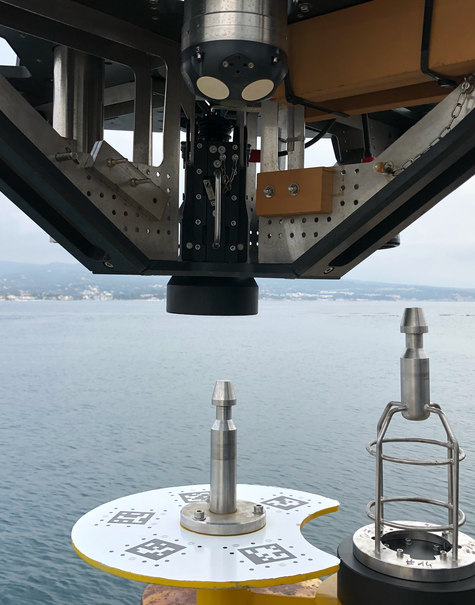
\includegraphics[width=0.99\textwidth]{imgs/latch_unlatched.png}
						\caption{Latch monté sur \atoll{} et crochet}
					\end{subfigure}
					\begin{subfigure}[b]{0.38\textwidth}
						\centering
						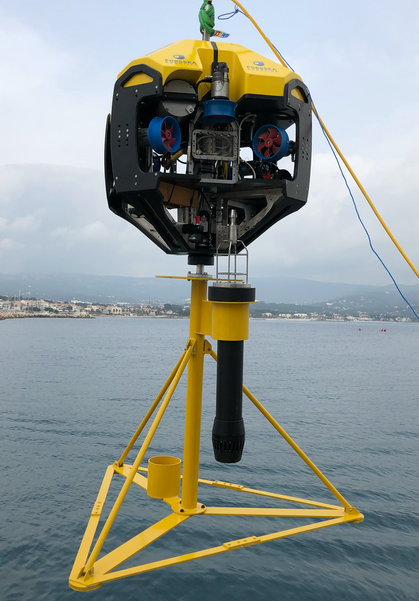
\includegraphics[width=\textwidth]{imgs/latch_latched.png}
						\caption{\atoll{} et structure sous-marine}
					\end{subfigure}
					\caption{Latch développé par \forssea{}}
					\label{fig:latch_photo}
				\end{figure}

				L'architecture logicielle du \textit{Latch} est présentée en \textsc{Figure}~\ref{fig:sa_latch}. Le composant reçoit deux informations de la part de l'implémentation logicielle : s'il est alimenté via le canal de communication \textit{power} et le signal de relâchement du crochet sur le canal \textit{release}. En retour, le crochet de levage renvoie son état à l'aide d'une sonde à effet hall qui indique si le crochet est fermé ou ouvert sur le canal \textit{sensor}.

				\begin{figure}[!htb]
					\centering
					\includegraphics[width=0.8\textwidth]{build/diagrams/sa_latch.pdf}
					\caption{Architecture logicielle du \textit{Latch}}
					\label{fig:sa_latch}
				\end{figure}
							
				Le \plugin{} \gazebo{} développé afin de décrire le comportement du \textit{Latch} est basé sur la machine à états finis présenté en \textsc{Figure}~\ref{fig:latch_fsm}. L'idée est de créer une liaison encastrement dynamique entre le \textit{Latch} et la structure sous-marine à transporter. La logique implémentée dans la machine à état finis permet de simuler le fait que mécaniquement le crochet s'accroche automatiquement à un point d'attache de structure sous-marine qui rentrerait dans le composant, et que l'on ne commande que le relâchement de cette structure par l'ouverture du crochet.

				\begin{figure}[!htb]
					\centering
					\includegraphics[scale=0.8]{build/diagrams/latch_fsm.pdf}
					\caption{Machine à états du \textit{Latch}}
					\label{fig:latch_fsm}
				\end{figure}

				On obtient alors le composant simulable dans l'environnement de simulation \gazebo{} et visualisable dans \rviz{} comme on peut le voir sur la \textsc{Figure}~\ref{fig:latch_gazebo_rviz}.

				\begin{figure}[!htb]
					\centering
					\caption{Simulation du Latch}
					\label{fig:latch_gazebo_rviz}
				\end{figure}
		
			\subsubsection{SS309 Tilt}

				Le \textit{SS309 Tilt} est un composant commercialisé par l'entreprise \textit{Sidus Solutions} et qui permet dans les \gls{ROV}s d'orienter la caméra d'observation. Il est parfaitement étanche et comporte un jeu d'engrenages reliés à un moteur pas-à-pas pilotable en vitesse et en position. On demande ainsi au moteur de mettre l'axe à une certaine position et l'axe se déplace avec une vitesse de rotation spécifiée. La \textsc{Figure}~\ref{fig:ss309_tilt} présente le composant monté sur \argos{} avec la nacelle peremttant de d'orienter la caméra d'observation.

				\begin{figure}[!htb]
					\centering
					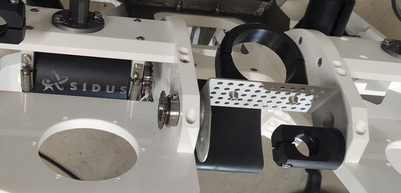
\includegraphics[width=0.6\textwidth]{imgs/ss309_tilt.png}
					\caption{SS309 tilt de \textit{Sidus Solutions} et nacelle pour \textit{Obscam}}
					\label{fig:ss309_tilt}
				\end{figure}
			
				Pour simuler cet aspect pilotable en vitesse de rotation et position, il faut passer par la simulation d'un moteur pas-à-pas. C'est un moteur composé de plusieurs bobinages créant ainsi plusieurs phases qui sont allumées successivement afin de réaliser une rotation de l'arbre moteur d'un certain incrément d'angle. Cet angle est défini par les caractéristiques du bobinage et n'est donc pas réglable. Ainsi, il est possible de connaître précisément la position du moteur, car l'arbre moteur ne peut prendre qu'un nombre fini d'angles, et il suffit donc de compter le nombre d'incréments commandés. Enfin, on peut commander la vitesse avec laquelle le moteur se rend à cette position, en allumant les phases à la vitesse désirée.

				L'architecture logicielle du \textit{SS309 Tilt} est présentée en \textsc{Figure}~\ref{fig:sa_tilt}. Le composant reçoit de la part de l'implémentation logicielle s'il est alimenté via le canal de communication \textit{power}, ainsi que la position et la vitesse consigne sur les canaux \textit{command/position} et \textit{command/velociy}. Il renvoie sa position et sa vitesse réelle récupérée dans l'environnement de simulation sur les canaux \textit{state/position} et \textit{state/velocity}.

				\begin{figure}[!htb]
					\centering
					\includegraphics[]{build/diagrams/sa_tilt.pdf}
					\caption{Architecture logicielle de la nacelle de caméra}
					\label{fig:sa_tilt}
				\end{figure}

				Nous allons à présent distinguer la position réelle de l'arbre moteur, la position cible et la position commandée. La position réelle est la position de l'arbre moteur dans le simulateur. La position cible est un multiple de l'incrément d'angle à laquelle doit se rendre le moteur à l'instant actuel. La position commandée la position finale dans laquelle doit se retrouver l'arbre moteur et peut être une position réelle quelconque. Le moteur ne sera capable que de se rendre à la position multiple de la valeur de l'incrément d'angle la plus proche de la position commandée. La \textsc{Figure}~\ref{fig:tilt_position} reprends ces différentes notions. En commandant la vitesse à laquelle on incrémente la position cible, on contrôle l'axe en vitesse.

				\begin{figure}[!htb]
					\centering
					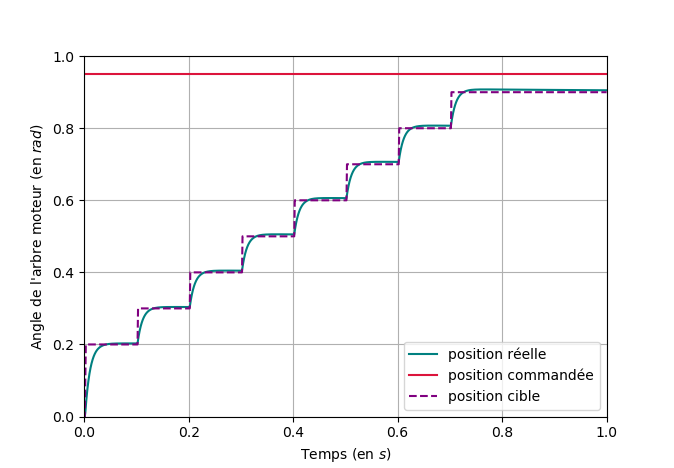
\includegraphics[width=0.6\textwidth]{imgs/stepper_motor.png}
					\caption{Simulation d'un moteur pas-à-pas}
					\label{fig:tilt_position}
				\end{figure}
				
				Pour ce qui est de l'implémentation de ce comportement dans \gazebo{}, on crée un \textit{Thread} qui va s'exécuter en boucle avec une vitesse variable. Cette vitesse sera fonction de la vitesse de commande du \textit{Tilt} notée $\omega_c$. A chaque tour de boucle, on incrémente donc la position cible de la valeur de l'incrément $d\theta$ si la différence entre la position réelle et la position commandée est plus grande que ce même incrément, et on attends le temps $h$, avec :

				$$h = \frac{d\theta}{\omega_c}$$

				\begin{algorithm}[!htb]
					\caption{Algorithme de simulation d'un moteur pas-à-pas}
					\label{algo:stepper_motor}
					\begin{algorithmic}
						\WHILE {true}
							\STATE read $\theta_r$, $\omega_c$
							\IF {$|\theta_c - \theta_r| > d\theta$}
								\STATE $\theta_t \leftarrow \theta_t + d\theta$
							\ENDIF
							\STATE $h \leftarrow \frac{d\theta}{\omega_c}$
							\STATE sleep $h$
						\ENDWHILE
					\end{algorithmic}
				\end{algorithm}

			\subsubsection{SPE75 Thrusters}
		
				Les \textit{SPE75 Thrusters} sont les propulseurs qui permettent aux robots de se déplacer et de s'orienter dans leur environnement. Ils sont composés d'un moteur permettant de mettre en mouvement des pales qui va permettre de générer une force dans la direction du propulseur.

				\begin{figure}[!htb]
					\centering
					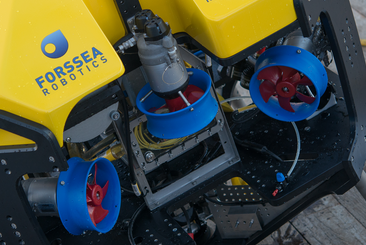
\includegraphics[width=0.6\textwidth]{imgs/spe75_thrusters.png}
					\caption{Trois propulseurs montés sur \atoll{}}
					\label{fig:thrusters}
				\end{figure}
				
				L'\textit{Hardware Interface} va proposer une interface aux contrôleurs permettant d'appliquer une force suivant l'axe du propulseur qui va être transmise au robot. Elle va ensuite se charger de calculer la vitesse de rotation des pales nécessaire à la création de cette force. Pour le composant réel, cette vitesse va être transmise au propulseur qui génère la force voulue et un couple résistant dans le sens inverse de la rotation des pâles sur le corps du propulseur qui va être transmis au robot. Pour le composant simulé, on est en mesure d'interagir avec le simulateur afin d'appliquer des forces et des couples directement sur les objets simulés. 
				
				Le calcul de la vitesse de rotation des pâles en fonction de la force demandée est réalisé grâce à une interpolation de points de mesures faits sur un banc d'essai. L'idée est de faire tourner en eau le propulseur fixé sur un capteur de force à une certaine vitesse, et de mesurer la force générée par celui-ci. Ensuite, on est capable d'interpoler les points expérimentaux logiciellement à l'aide de la librairie \textit{GSL}\footnote{\url{https://www.gnu.org/software/gsl/}} et de la fonctionnalité \textit{spline}. On peut ainsi calculer une vitesse de rotation à appliquer quelle que soit la valeur de force demandée.
				
				L'idée retenue pour ce simulateur est d'appliquer directement la force demandée sur le corps du propulseur, car il est assez difficile et coûteux en ressources de calculs de réaliser de la mécanique des fluides afin de simuler pleinement le comportement des pâles du propulseur. Il est tout de même nécessaire de faire tourner les pâles dans le simulateur, car outre l'aspect cosmétique de voir les pales tourner quand le moteur fournit une poussée au robot, le simple fait de faire tourner ce solide ayant une certaine masse dans le simulateur va générer le couple résistant sur le corps du propulseur. Ainsi cette \textit{Hardware Interface} va communiquer au \textit{Model Plugin} la force et la vitesse de rotation des pâles calculée à appliquer sur le propulseur simulé.
	
				Le \textit{Model Plugin} va se charger d'appliquer la force et la vitesse de rotation communiquée par l'\textit{Hardware Interface}. Le \textit{plugin} est chargé pour chaque propulseur simulé et permet d'accéder finement aux paramètres de la simulation. On peut alors appliquer à chaque incrément de simulation la force demandée sur le corps du propulseur et la vitesse de rotation sur la liaison pivot entre le corps du propulseur et les pâles.

	\section{Simulation des robots}

		\subsection{Description du robot}

		\subsection{Tests unitaires}
				
			Il est nécessaire de vérifier si tous les composants fonctionnent correctement et ont été convenablement ajoutés dans le robot. Pour cela il est courant d'implémenter des tests unitaires., qui vont permettre de tester unitairement les différentes fonctionnalités implémentées. Il est aussi nécessaire d'ajouter des tests liés au choix de conception que nous avons fait, c’est-à-dire le fait d'avoir séparé les robots en composants simulés indépendamment les uns des autres.

			En effet, nous avons créé une description des \gls{ROV}s en incluant la description des sous-composants nécessaires. Il faut maintenant vérifier que la masse du robot, la position de son centre de gravité, sa matrice d'inertie, son volume et son centre de volume correspondent bien aux paramètres des robots. Pour ce faire, nous allons interpréter le fichier de description \textit{URDF} des robots en utilisant le module python \textit{urdfpy}\footnote{\url{https://github.com/mmatl/urdfpy}} afin de vérifier ces informations.

			\subsubsection{Vérification de la masse}

				Pour calculer la masse totale du robot, il suffit de sommer la masse de tous les composants. En considérant que le robot possède \textit{N} composants, et que $\forall i \in \llbracket 1; N \rrbracket, m_i$ représente la masse du \textit{i-ème} composant, et $m_{robot}$ la masse du robot, on a :

				\begin{equation}
					m_{robot} = \sum_{i=0}^{N}m_i
				\end{equation}

			\subsubsection{Vérification du centre de gravité}

				Pour calculer le centre de gravité du robot, on réalise une moyenne des centres de gravités pondérée par les masses des différents composants. En considérant que le robot possède \textit{N} composants, et que $\forall i \in \llbracket 1; N \rrbracket, m_i$ représente la masse du \textit{i-ème} composant et $G_i$ représente les coordonnées de son centre de gravité dans le repère monde, et $G_{robot}$ le centre de gravité du robot, on a :

				\begin{equation}
					G_{robot} = \frac{\sum_{i=0}^{N}m_i.G_i}{\sum_{i=0}^{N}m_i}
				\end{equation}

			\subsubsection{Vérification de la matrice d'inertie}

				Pour calculer la matrice d'inertie du robot, il faut sommer les inerties du robot. Définissons le repère $R_0$ associé au châssis du robot et le repère $R_i$ associé au composant \textit{i}. Partons de la matrice d'inertie disponible dans la description \textit{URDF} du robot exprimées dans le repère de chaque composant et en leur centre de gravité. Notons cette matrice $I_{i, R_i}(G_i)$. 
				
				Par cinématique directe, on peut obtenir la matrice de la transformation homogène $H_0^i$ entre les repères $R_0$ et $R_i$, qui exprime la rotation et la translation entre ces deux repères. Cette matrice est composée d'une matrice de rotation $R_{3, 3}$ et d'une matrice traduisant la translation $T_{3, 1}$ entre les deux solides.

				\begin{equation}
					H_{R_0}^{R_i} = \begin{bNiceArray}{CCC:C}[margin] &&& \\ & R_{3, 3} && T_{3, 1} \\ &&& \\ \hdottedline 0 & 0 & 0 & 1 \end{bNiceArray}
				\end{equation}

				En notant $I_{i, R_0}(G_i)$ la matrice d'inertie du i-ème composant exprimée en son centre de gravité dans le repère associé au châssis du robot, on peut exprimer le changement de base du tenseur d'inertie comme suit :

				\begin{equation}
					I_{i, R_0}(G_i) = R^T.I_{i, R_i}(G_i).R
				\end{equation}

				Puis, il faut exprimer le décalage entre l'origine du robot et le centre de gravité du composant. En utilisant la convention des coordonnées homogènes, et en notant $d^H = \begin{bmatrix}a & b & c & 1\end{bmatrix}^T$, on a :

				\begin{equation}
					d^H = H_0^i . G_i^H
				\end{equation}

				Ensuite on peut déplacer ce tenseur à l'origine du repère \textit{0} à l'aide de la formule de \textit{König-Huygens} :

				\begin{equation}
					I_{i, R_0}(O) = I_{i, R_0}(G_i) + m_i.\begin{bmatrix} b^2 + c^2 & -a.b & -a.c \\ -a.b & a^2 + c^2 & -b.c \\ -a.c & -b.c & a^2 + b^2 \end{bmatrix}
				\end{equation}

				Enfin, en possédant le tenseur d'inertie de chaque composant dans la base \textit{0} et au même point qui est l'origine du robot, on est en mesure de sommer ces inerties pour obtenir l'inertie totale du robot.

				\begin{equation}
					I_{robot, R_0}(O) = \sum_{i=0}^N I_{i, R_0}(O)
				\end{equation}

			\subsubsection{Vérification du volume}

				Pour calculer le volume total du robot, il suffit de sommer le volume de tous les composants. En considérant que le robot possède \textit{N} composants, et que $\forall i \in \llbracket 1; N \rrbracket, v_i$ représente le volume du \textit{i-ème} composant, et $v_{robot}$ le volume du robot, on a :

				\begin{equation}
					v_{robot} = \sum_{i=0}^{N}v_i
				\end{equation}

			\subsubsection{Vérification du centre de volume}

				Pour calculer le centre de volume du robot, on réalise une moyenne des centres de volume pondérée par le volume des différents composants. En considérant que le robot possède \textit{N} composants, et que $\forall i \in \llbracket 1; N \rrbracket, v_i$ représente le volume du \textit{i-ème} composant, $V_i$ représente les coordonnées du centre de volume dans le repère du robot, et $V_{robot}$ le volume du robot, on a :

				\begin{equation}
					V_{robot} = \frac{\sum_{i=0}^{N}v_i.V_i}{\sum_{i=0}^{N}v_i}
				\end{equation}


		\subsection{Tests unitaires d'\argos{}}

			Les différents tests unitaires ont été lancés sur les fichiers de descriptions \textit{URDF} d'\argos{} afin de vérifier que la composition du robot à base des différents composants définis ait bien les bonnes propriétés mécaniques. La \textsc{Table}~\ref{table:argos_unittest} présente les écarts entre le robot réel et la description réalisée à l'aide des composants. On y retrouve ainsi les résultats des tests unitaires pour \argos{}.
			
			\begin{table}[!htb]
				\centering
				\begin{adjustbox}{max width=\textwidth}
					\begin{tabular}{|c|c|c|c|c|}
						\hline
						\textbf{Grandeurs} & \textbf{Ecart avec la réalité} & \textbf{Marge d'erreur acceptée} & \textbf{Validation} \\
						\hline
						Masse (en $kg$) & $0.66$ & $\pm 1$ & \cmark \\
						\hline
						Position du Centre de Gravité (en $mm$) & $0.3 \quad 0.1 \quad 0.2$ & $\pm 1 \quad \pm 1 \quad \pm 1$ & \cmark \\
						\hline
						Matrice d'Inertie (en $m^2.kg$) & $\begin{bmatrix}0.2 & 0.03 & 0.11 \\ 0.03 & 0.23 & 0.08 \\ 0.11 & 0.08 & 0\end{bmatrix}$ & $\pm \begin{bmatrix}0.3 & 0.15 & 0.15 \\ 0.15 & 0.3 & 0.15 \\ 0.15 & 0.15 & 0.3\end{bmatrix}$ & \cmark \\
						\hline
						Volume (en $m^3$) & $0.1656$ & $\pm 0.005$ & \cmark \\
						\hline
						Position du Centre de Volume (en $mm$) & $1 \quad 1 \quad 1$ & $\pm 0.05 \quad \pm 0.05 \quad \pm 0.05$ & \cmark \\
						\hline
					\end{tabular}
				\end{adjustbox}
				\caption{Tests unitaires d'\argos{}}
				\label{table:argos_unittest}
			\end{table}

			On voit que toutes les valeurs des écarts entre le robot réel et la description \textit{URDF} sont inférieures aux marges d'erreurs acceptables pour \argos{}, ce qui signifie que les tests unitaires sont bien validés pour ce robot.

		\subsection{Tests unitaires d'\atoll{}}

			Les différents tests unitaires ont été lancés sur les fichiers de descriptions \textit{URDF} d'\atoll{} afin de vérifier que la composition du robot à base des différents composants définis ait bien les bonnes propriétés mécaniques. La \textsc{Table}~\ref{table:atoll_unittest} présente les écarts entre le robot réel et la description réalisée à l'aide des composants. On y retrouve ainsi les résultats des tests unitaires pour \atoll{}.
			
			\begin{table}[!htb]
				\centering
				\begin{adjustbox}{max width=\textwidth}
					\begin{tabular}{|c|c|c|c|c|}
						\hline
						\textbf{Grandeurs} & \textbf{Ecart avec la réalité} & \textbf{Marge d'erreur acceptée} & \textbf{Validation} \\
						\hline
						Masse (en $kg$) & $0.66$ & $\pm 1$ & \cmark \\
						\hline
						Position du Centre de Gravité (en $mm$) & $0.3 \quad 0.1 \quad 0.2$ & $\pm 1 \quad \pm 1 \quad \pm 1$ & \cmark \\
						\hline
						Matrice d'Inertie (en $m^2.kg$) & $\begin{bmatrix}0.2 & 0.03 & 0.11 \\ 0.03 & 0.23 & 0.08 \\ 0.11 & 0.08 & 0\end{bmatrix}$ & $\pm \begin{bmatrix}0.3 & 0.15 & 0.15 \\ 0.15 & 0.3 & 0.15 \\ 0.15 & 0.15 & 0.3\end{bmatrix}$ & \cmark \\
						\hline
						Volume (en $m^3$) & $0.1656$ & $\pm 0.005$ & \cmark \\
						\hline
						Position du Centre de Volume (en $mm$) & $1 \quad 1 \quad 1$ & $\pm 0.05 \quad \pm 0.05 \quad \pm 0.05$ & \cmark \\
						\hline
					\end{tabular}
				\end{adjustbox}
				\caption{Tests unitaires d'\atoll{}}
				\label{table:atoll_unittest}
			\end{table}

			On voit que tous les valeurs des écarts entre le robot réel et la description \textit{URDF} sont inférieures aux marges d'erreurs acceptables pour \argos{}, ce qui signifie que les tests unitaires sont bien validés pour ce robot.

	\section{Conclusion}
	
		En conclusion, nous avons divisé le travail de simulation des robots en simulant les composants uns à uns, afin de simplifier les développements et de mettre en commun un maximum de code entre les \gls{ROV}s. Pour la plupart des composants, un \plugin{} \gazebo{} a été nécessaire afin de décrire leur comportement dans l'environnement de simulation, et de pouvoir contrôler les robots avec le reste de l'implémentation logicielle. Enfin, nous nous sommes assurés que la simulation en composants donnait bien des paramètres mécaniques corrects pour les robots simulés par rapport au robot réel, afin d'avoir une simulation des robots ayant un comportement proche des \gls{ROV}s en conditions réelles.

	\chapter{Résultats}
\chaptermark{Résultats}
\label{chapter:resultats}
	
	\section{Introduction}

		Nous avons désormais implémenté tous les éléments de notre simulateur, et nous allons donc pouvoir à présent tester le bon fonctionnement de notre système au complet afin d'analyser les résultats produits. Cela va nous permettre de tester que toutes les implémentations logicielles s'interfacent bien toutes ensemble et que le simulateur a un comportement physique correct.
		
		Dans un premier temps, nous allons vérifier que le système respecte les exigences présentées dans le \textsc{Chapitre}~\ref{chapitre:systeme}, ainsi que le comportement des robots et de l'environnement développés dans les \textsc{Chapitre}~\ref{chapitre:environnement} et \textsc{Chapitre}~\ref{chapitre:robots}.

		Ensuite, nous nous pencherons sur la comparaison du simulateur avec des expérimentations faites avec les \gls{ROV}s \argos{} et \atoll{}, afin de déterminer si les résultats de simulations sont proches du comportement réel des robots, et si ce système permettrait bien de réduire les temps de développements en réduisant le nombre d'essais en conditions réelles à réaliser pour valider de nouvelles fonctionnalités.

	\section{Analyse du simulateur}

		\subsection{Visualisation des robots}

			\gls{ROS2} propose un outil qui permet de visualiser les robots et les données fournies par les capteurs, c'est le logiciel \gls{RViz2}. Il est systématique de retrouver dans les packages de description de robots pour \gls{ROS2} de retrouver un fichier de configuration permettant de visualiser le robot dans \gls{RViz2}, et c'est pourquoi c'est une fonctionnalité 

		\subsection{Invocation des robots dans l'environnement de simulation}

			Le premier test à réaliser est sûrement d'invoquer les robots dans le monde sous-marin afin de tester l'interaction des robots avec leur milieu. Il faut que le robot ait un comportement physique avec l'environnement de simulation qui soit acceptable. Globalement le robot doit avoir une flottabilité quasiment nulle, mais légèrement positive, afin qu'il remonte naturellement en cas de problème avec les propulseurs.

			On vérifie que les robots sont bien 

	\section{Comparaison avec les robots réels}

		Ecarts (statique/dynamique) lors d'essais en bassins ou réels

		\begin{figure}
			\includegraphics{build/imgs/rosace_local.pdf}
			\caption{Rosace réalisée par Argos}
			\label{fig:rosace_argos}
		\end{figure}

	\section{Conclusion}
	\chapter{Gestion de projet}
\chaptermark{Projet}
\label{chapter:projet}
	
	\section{Introduction}

		Ce dernier chapitre est consacré à la gestion de projet. Elle est nécessaire à la réalisation d'un système et cela prend une place importante dans la démarche de l'ingénieur. Nous allons ici présenter les différentes méthodes et outils mis en place qui ont été nécessaire au bon déroulement de ce projet de fin d'études.

		Le format de ce projet de fin d'études est particulier dans la mesure où j'ai réalisé la dernière année de ma formation en contrat de professionnalisation avec l'entreprise Forssea Robotics. J'ai donc pu travailler pendant une année complète à leurs côtés, en commençant par 6 mois durant lesquels j'ai fini ma formation au sein de l'\gls{ENSTAB}, puis 6 mois durant lesquels j'ai pu travailler à temps plein sur mon projet de fin d'études. Cela a présenté l'avantage d'avoir à ma charge la gestion d'un projet plus complet, puisque le temps l'a permis, comparé à un projet de fin d'étude classique dans lequel il est souvent confié au stagiaire la réalisation d'une tâche d'un projet.

	\section{Méthodologie}

		\subsection{Méthodes Agiles}
			Les \textit{Méthodes Agiles} forment un ensemble de méthodes facilitant la gestion de projet, qui sont particulièrement adaptées au monde du développement logiciel. Il permet de réaliser une planification adaptative, un développement évolutif et une amélioration continue du produit. Elles s'opposent aux méthodes plus traditionnelles, comme les méthodes séquentielles de type \textit{Cycle en V}, qui s'adaptent très mal à ce type de système. Elles permettent aussi d'avoir un produit utilisable par le client, avec des fonctionnalités qui évoluent au cours du développement.

			La \textit{Méthode Scrum} est un cadre hérité de la \textit{Méthode Agile} permettant lui aussi de gérer le développement d'un produit. Cette méthode se distingue des \textit{Méthodes Agiles} dans la mesure où ce n'est pas seulement un ensemble de concepts, mais plutôt ici un ensemble de règles à suivre pour gérer correctement un projet. La \textit{Méthode Scrum} nécessite la désignation de :

			\begin{itemize}
				\item Un \textit{Scrum Master} : garant de l'application de la \textit{Méthode Scrum},
				\item Un \textit{Product Owner} : garant des attentes du client au sein du projet,
				\item Une équipe de développement : réalisant le produit.
			\end{itemize}

			Les temps forts de la \textit{Méthode Scrum} sont :

			\begin{itemize}
				\item La plannification de \textit{sprint} : réunion durant laquelle les nouvelles fonctionnalités à ajouter au produit sont sélectionnées en accord avec le \textit{Product Owner},
				\item La revue de \textit{sprint} : réunion se déroulant en général après le sprint et durant laquelle les nouvelles fonctionnalités implémentées durant le \textit{sprint} sont présentées au \textit{Product Owner} et au client, et le prochain sprint est préparé,
				\item La rétrospective de \textit{sprint} : réunion dans laquelle l'équipe analyse sa propre gestion de projet en terme d'efficacité, de qualité, de productivité,
				\item La mêlée quotidienne : réunion dans laquelle l'équipe de développement expose ce qu'elle a réalisé, ce qu'elle va réaliser et les problèmes qui ont été rencontrés depuis la dernière mêlée.
			\end{itemize}
		
			Lors du développement du simulateur réalisé pendant ce projet de fin d'étude, une \textit{Méthode Scrum} a été utilisée, dans la mesure où c'est la méthode qui est utilisée par le reste de l'entreprise. On peut cependant la qualifier de légère, car les \textit{sprints} n'étaient pas très formalisés, d'abord car j'étais le seul développeur en charge de ce projet de simulation. Le choix des nouvelles fonctionnalités à prendre en compte était décidé lors d'une réunion hebdomadaire servant de point d'avancement du produit. Les réunions quotidiennes étaient cependant bien présente, et elle permettaient d'avoir à l'esprit ce que les autres développeurs étaient en train de faire. En outre la start-up est divisée en trois pôles : Robotique, Vision et Mécanique. Les réunions quotidiennes étaient séparées par pôles afin d'être plus efficace, mais une réunion mensuelle venait synchroniser les différentes équipes afin de définir les objectifs réalisés et à venir pour l'entreprise.

	\section{Outil de gestion de projet}

		\subsection{GitHub}

			Le service \textit{Github}\footnote{\url{https://github.com/}} permet de versionner et de travailler facilement en collaboration sur de l'implémentation logicielle. Basé sur le logiciel de versionnage \textit{Git}\footnote{\url{https://git-scm.com/}}, ce service propose la possibilité de créer des organisations, et donc d'avoir une entité associée à la société \textit{Forssea Robotics} possédant tout le code implémenté.

			L'entreprise utilise le \textit{Git Flow} qui est une bonne pratique d'utilisation de \textit{Git}. Elle définit un certain nombre de branches ayant un rôle précis :

			\begin{itemize}
				\item La branche \textit{master} : branche délivrable au client contenant la dernière version du code,
				\item La branche \textit{develop} : branche contenant les développements liés à la prochaine version où sont fusionnés les fonctionnalités à venir développés par les différents développeurs,
				\item Les branches de \textit{features} : branches d'implémentation de fonctionnalités. Il y en a autant que de fonctionnalités à ajouter, et chaque développeur autant de branches qu'il a besoin au cours de l'implémentation,
				\item La branche \textit{release} : branche sur laquelle est testé le contenu de la branche \textit{develop} avant la livraison de la nouvelle version sur la branche \textit{master},
				\item La branche \textit{hotfix} : branche sur laquelle des corrections mineures et urgentes peuvent être apportées sur la branche \textit{master}.
			\end{itemize}

			Je trouve cette méthodologie intéressante, car elle propose un ensemble de règles à respecter afin de gérer convenablement le développement logiciel d'un produit. C'est quelque chose que je ne connaissais pas auparavant, mais que je n'hésiterais pas à remettre en place dans mes futurs développements.

		\subsection{Jira}

			Un outil intéressant pour appliquer la \textit{Méthode Scrum} est le service \textit{Jira} d'\textit{Atlassian}\footnote{\url{https://www.atlassian.com/fr/software/jira}}. C'est un outil développé pour appliquer ces méthodes de gestion de projet en équipe, avec une intégration des différents concepts et des différentes règles inhérentes à ces procédés. Il permet de facilement planifier le projet, le suivre, mais aussi de livrer facilement et de créer des rapports de fonctionnalités, des notes de versions et autres notices utiles pour l'utilisateur final.
		
			Le suivi d'implémentation est automatisé entre \textit{Jira} et \textit{Github} : dès qu'une nouvelle fonctionnalité est ajoutée sur \textit{GitHub}, elle est automatiquement classée comme implémentée sur \textit{Jira}. Ainsi la \textit{Roadmap}\footnote{Planning dans lequel figurent les développements en cours ainsi que leurs durées} est tenue à jour et il est possible de se rendre compte de l'intention stratégique prise par les développements en cours ainsi que des délais prévus.

			Un système de tests unitaires permettent aussi de tester en intégration le code implémenté, afin d'être sûr que le code est fonctionnel. En outre, ces test unitaires servent de tests de non régressions pour les versions suivantes afin de vérifier que les prochaines versions logicielles ne changeront pas les comportements implémentés dans les précédentes versions.

		\subsection{Clockify}
			
			Clockify est un logiciel permettant de gérer les temps de développements. Il s'intègre lui aussi parfaitement avec \textit{Jira} et permet de se rendre compte du temps passé sur chaque tâche. Il suffit de démarrer un chronomètre directement dans \textit{Jira}, et le temps commence à s'écouler. A la fin d'un développement, on arrête le chronomètre en appuyant sur le bouton stop, et le temps est automatiquement additionné. On a donc une \textit{Roadmap} mise à jour régulièrement, et une idée des ressources qui ont été allouées pour le projet.

		\subsection{Etude de faisabilité et solution technique}

			La réalisation de chaque tâche passe par la rédaction d'une étude de faisabilité et la présentation de la solution technique, abrégé \textit{FTS}\footnote{\textit{Feasibility and Technical Solution}}. Ce document est souvent accompagné d'une \textit{POC}\footnote{\textit{Proof Of Concept}}, qui est un exemple minimal de code prouvant que le concept à implémenter est faisable et que la solution répond bien au besoin. Cela permet de ne pas passer du temps de développement sur une solution non satisfaisante.

			La simulation de l'ombilical par exemple est la tache qui a nécessité le plus de préparation. Etant donné que la simulation dans \textsc{Gazebo} d'un ombilical par éléments finis n'avait jamais été fait auparavant, la rédaction de la \textit{FTS} et la \textit{POC} ont nécessité quelques mois de développements. J'ai pu réaliser ce travail préalable en parallèle de la fin de ma formation, durant les six premiers mois de contrat de professionnalisation. Cela a permis d'éclaircir quelques points qui semblaient triviaux à implémenter, mais qui ont finalement soulevés des problèmes nécessitant du temps de développement. 
			
			Cependant, on remarque que certains problèmes se sont tout de même présentés lors de l'implémentation de cette solution dans \gazebo{}. C'est le cas de l'orientation absolue des solides qui était accessible dans le code développé pour la \textit{POC}, alors que dans le \textit{plugin} implémenté pour le simulateur, seul les orientations relatives ramenées dans l'intervalle $[-\pi; \pi]$ étaient accessible.

		\subsection{Diagramme de Gantt}
			
			Pour gérer convenablement ce projet, un diagramme de Gantt prévisionnel a été mis en place au début de ce projet. Il a permis d'organiser le temps de ce stage afin de pouvoir mener à bien la réalisation de ce projet. Il a ensuite été mis à jour régulièrement afin de prendre en compte les différents changements et imprévus survenus au cours de cette année. Ces deux diagrammes sont disponibles en \textsc{Annexe}~\ref{annexe:gantt}, et permettent de se rendre compte de l'évolution du projet au cours de son développement.

	\section{Conclusion}
	
		Ce projet de fin d'étude m'a permis de découvrir un bon nombre d'outils qui se sont avérés être indispensable dans la gestion de projet. De plus, j'ai pu appliquer des méthodes agiles de gestion de projet au sein de l'équipe robotique de \textit{Forssea Robotics}, qui sont des méthodes très utilisées dans le domaine de la robotique.
	\chapter{Conclusion}
	\label{chapitre:conclusion}
	
	\section{Conclusion technique}

		La réalisation de ce simulateur est un point très important dans le domaine du développement robotique. Je suis conscient des gains apportés par un tel système en terme de coûts de développements, car les essais en robotique restent très onéreux, la puissance de calculs de nos ordinateurs sont aujourd'hui largement suffisantes, et les logiciels de simulations de plus en plus complets et puissants. 
		
		Un exemple marquant est que durant mon projet de fin d'études, une semaine d'essais prévue n'a quasiment servie à rien, car le bateau censé être utilisé pour la campagne d'essais n'a pas pu quitter le port à cause d'un problème météorologique. Cela a nécéssairement mobilisé du matériel et des hommes pour tester des fonctionnalités qui auraient pu être testée en simulation dans un premier temps, avant de réaliser une campagne d'essais finale permettant de valider la nouvelle version complète du robot.
	
	\section{Conclusion du projet}

		Ce simulateur a été réalisé durant un contrat de professionnalisation avec \textsc{Forssea Robotics} et dans la continuité de mon stage de deuxième année réalisé aussi sur des aspect de simulation en développement robotique sur \gls{Gazebo} dans la jeune pousse \textsc{Exxact Robotics}. J'ai donc pu me spécialiser cette dernière année dans la simulation robotique et notamment sur l'utilisation du simulateur \gls{Gazebo} qui est très permissif et dans lequel j'ai pu beaucoup apprendre.

		En terme de gestion de projets, il a été très intéressant d'avoir à ma charge la gestion de l'intégralité du projet simulation. Je trouve que c'est une bonne introduction à mon futur parcours professionnel, et l'encadrement de mon maître de stage m'a permis de mener à bien ce projet.

		La conception de ce système m'a amené à formaliser beaucoup d'aspects du simulateur, et le côté start-up de \textsc{Forssea Robotics} fait que les projets sont axés recherche et développement. Cela a éveillé en moi un attrait pour la recherche et m'incite à continuer mes études dans le monde de la recherche par la réalisation d'une thèse à la suite de ce projet de fin d'études.
	
	\appendix
	\cleardoublepage
	\pagenumbering{roman}
	\chapter{Annexes}
\label{annexe:gantt}

	\section{Simplification en eaux profondes}

		Nous allons ici justifier la simplification faite en eaux profondes dans la \textsc{Section}~\ref{sec:simplification_eaux_profondes}. Nous avons en effet pu proposer une approximation en \textsc{Equation}~\ref{eqn:simplification_eaux_profondes} qui permet de simplifier les équations décrivant la dynamique du milieu marin.

		\begin{eqnarray}
			\frac{cosh(k_m(z+H))}{sinh(k_mH)} = \left( \frac{e^{z+H} + e^{-z+H}}{e^{H}-e^{-H}} \right)^{k_m}  \xrightarrow[H \rightarrow + \infty]{}   \left( \frac{e^{z+H}}{e^{H}} \right)^{k_m} = e^{k_m z}
		\end{eqnarray}

	\clearpage

	\begin{figure}[H]
		\centering
		\rotatebox{90}{
			\includegraphics[width=21cm]{gantt_before.pdf}
		}
        \label{fig:gantt_before}
        \caption{Diagramme de Gantt prévisionnel du projet}
	\end{figure}

	\begin{figure}[H]
		\centering
		\rotatebox{90}{
			\includegraphics[width=21cm]{gantt_after.pdf}
		}
        \label{fig:gantt_after}
        \caption{Diagramme de Gantt final du projet}
	\end{figure}

	\clearpage
	\phantomsection
	\label{chapter:lof}
	\addcontentsline{toc}{chapter}{Liste des figures}
	\listoffigures

	\clearpage
	\phantomsection
	\label{chapter:lot}
	\addcontentsline{toc}{chapter}{Liste des tables}
	\listoftables

	\clearpage
	\phantomsection
	\label{sec:glossaire}
	\printglossaries

	\clearpage
	\phantomsection
	\addcontentsline{toc}{chapter}{Bibliographie}

	\bibliography{bib/sea,bib/intro,bib/software.bib,bib/tether.bib}
	\bibliographystyle{ieeetr}
\end{document}
